% ============================================================================
% COMPREHENSIVE PREAMBLE FOR ERDOS PROBLEM 915 THESIS
% ============================================================================

\documentclass[kul, 11pt, a4paper, oneside]{kulakreport}
\usetikzlibrary{calc, arrows.meta, shapes.geometric, decorations.markings}

% KU Leuven metadata
\faculty{Faculty of Science}
\group{Department of Mathematics}
\subtitle{Erd\H{o}s Problem 915, from Proof to Search}
\institute{Master of Mathematics}
\emailaddress{louis.vandenbruwaene@student.kuleuven.be}
\address{
   \textbf{KU Leuven} \\
   \textbf{Faculty of Science} \\
   Celestijnenlaan 200B, 3001 Leuven \\
   Belgium
}

% ============================================================================
% BASIC PACKAGES
% ============================================================================
\usepackage[utf8]{inputenc}
\usepackage[T1]{fontenc}
\usepackage[scaled=0.95]{helvet}
\renewcommand{\familydefault}{\sfdefault}
\usepackage[absolute,overlay]{textpos}
% lmodern not available; disable microtype expansion to avoid font errors
\usepackage[patch=none, expansion=false]{microtype}

% ============================================================================
% PAGE LAYOUT
% ============================================================================
\usepackage[
    a4paper,
    inner=25mm,
    outer=25mm,
    top=30mm,
    bottom=30mm,
    bindingoffset=5mm
]{geometry}

\usepackage{setspace}
\onehalfspacing

% Improve line breaking to reduce overfull hbox warnings
\tolerance=1414
\emergencystretch=1.5em
\hfuzz=3pt
\vfuzz=3pt

% ============================================================================
% MATHEMATICS
% ============================================================================
\usepackage{amsmath, amssymb, amsthm}
\usepackage{mathtools}
\usepackage{bm}

% ============================================================================
% GRAPHICS AND COLOR (tikz, graphicx, xcolor already loaded by kulakreport)
% ============================================================================
\usetikzlibrary{positioning, arrows.meta, calc, shapes.geometric,
                decorations.pathmorphing, backgrounds, fit,
                patterns, shadows, matrix}

% ============================================================================
% FIGURES AND TABLES
% ============================================================================
\usepackage{float}
% rotating: the twelve-panel bounds grid needs a full sideways page, since at
% text width its per-panel labels fall under 2pt.
\usepackage{rotating}
\usepackage{caption}
\usepackage{subcaption}
\usepackage{booktabs}
\usepackage{array}
\usepackage{multirow}

% Uniform caption look for every plot, figure, and table: a bold blue label, a
% slightly smaller justified body set in from the margins, and a touch of space
% above so a caption never crowds the artwork it describes.
\captionsetup{
    font=small,
    labelfont={bf,color=KULblauw3b},
    textfont={color=black!85},
    labelsep=period,
    justification=justified,
    singlelinecheck=true,
    margin=14pt,
    skip=8pt,
}
\captionsetup[sub]{
    font=footnotesize,
    labelfont={bf,color=KULblauw3b},
    % Ragged right, not justified: sub-captions often sit in narrow boxes
    % (half-width panels), where justification stretches short lines into
    % wide word gaps around unbreakable math.
    justification=raggedright,
    margin=4pt,
    skip=5pt,
}

% ============================================================================
% LISTS
% ============================================================================
\usepackage{enumitem}

% Custom bullet styles using small graph icons
\newcommand{\prettygrotzsch}{%
	\tikz[baseline=-0.6ex, scale=0.12]{
		\definecolor{nodecolor}{RGB}{50, 120, 180}
		\foreach \i in {0,...,4} {
			\coordinate (inner\i) at ({1.2*cos(72*\i+18)},{1.2*sin(72*\i+18)});
		}
		\coordinate (center) at (0,0);
		\draw[nodecolor, line width=0.5pt]
		(center) -- (inner0) (center) -- (inner1) (center) -- (inner2)
		(center) -- (inner3) (center) -- (inner4)
		(inner0) -- (inner2) (inner0) -- (inner3) (inner1) -- (inner3)
		(inner1) -- (inner4) (inner2) -- (inner4);
		\foreach \i in {0,...,4} { \fill[black] (inner\i) circle (2.5pt); }
		\fill[black] (center) circle (2.5pt);
	}
}

\newcommand{\prettypetersen}{%
	\tikz[baseline=-0.6ex, scale=0.15]{
		\definecolor{petersennode}{RGB}{20, 140, 140}
		\definecolor{petersenedge}{RGB}{100, 100, 100}

		\def\R{1.2}
		\def\r{0.8}

		\foreach \i in {0,...,4} {
			\coordinate (outer\i) at ({90+72*\i}:\R);
			\coordinate (inner\i) at ({90+72*\i}:\r);
		}

		\foreach \i in {0,...,4} {
			\fill[petersennode] (outer\i) circle (4pt);
			\fill[petersennode] (inner\i) circle (4pt);
		}

		\draw[petersenedge, line width=0.7pt]
		(outer0) -- (outer1) -- (outer2) -- (outer3) -- (outer4) -- (outer0)
		(outer0) -- (inner0)
		(outer1) -- (inner1)
		(outer2) -- (inner2)
		(outer3) -- (inner3)
		(outer4) -- (inner4)
		(inner0) -- (inner2) -- (inner4) -- (inner1) -- (inner3) -- (inner0);

		\foreach \i in {0,...,4} {
			\fill[black, opacity=1] (outer\i) circle (3pt);
			\fill[black, opacity=1] (inner\i) circle (3pt);
		}
	}
}

\setlist[itemize]{label=$\prettygrotzsch$, leftmargin=1.5em}
\setlist[enumerate]{label=\protect\prettypetersen, leftmargin=2em}

% ============================================================================
% HYPERLINKS AND REFERENCES
% ============================================================================
\usepackage[noabbrev, capitalize, nameinlink]{cleveref}

% ============================================================================
% BIBLIOGRAPHY
% ============================================================================
\usepackage[numbers, sort&compress]{natbib}

% ============================================================================
% HEADER/FOOTER
% ============================================================================
% The page footer ("section mark | page number") is defined by the kulakreport
% class with oneside-friendly specifiers; nothing to add here.

% ============================================================================
% CHAPTER STYLING
% ============================================================================
\usepackage{titlesec}
% Chapter: keep the large black title, but brand the "Chapter N" label in the
% KU Leuven house blue so the heading reads as part of the institutional style.
\titleformat{\chapter}[display]
  {\normalfont\huge\bfseries}{\color{KULblauw1}\chaptertitlename\ \thechapter}{20pt}{\Huge\raggedright}
\titlespacing*{\chapter}{0pt}{-30pt}{40pt}

% Section headings: black bold title with a blue section number and a thin blue
% accent rule beneath, matching the chapter branding and easing navigation in
% the long chapters. Subsection and below stay quieter, with only a blue number.
\titleformat{\section}
  {\normalfont\Large\bfseries}{\color{KULblauw1}\thesection}{0.7em}{}
\titlespacing*{\section}{0pt}{1.8ex plus .3ex minus .2ex}{0.9ex}

\titleformat{\subsection}
  {\normalfont\large\bfseries}{\color{KULblauw1}\thesubsection}{0.6em}{}
\titlespacing*{\subsection}{0pt}{1.4ex plus .2ex minus .2ex}{0.6ex}

\titleformat{\subsubsection}
  {\normalfont\normalsize\bfseries}{\color{KULblauw1}\thesubsubsection}{0.5em}{}
\titlespacing*{\subsubsection}{0pt}{1.1ex plus .2ex minus .2ex}{0.5ex}

\titleformat{\paragraph}[runin]
  {\normalfont\normalsize\bfseries\color{KULblauw3b}}{}{0pt}{}
\titlespacing*{\paragraph}{0pt}{1ex plus .2ex minus .1ex}{0.8em}

% Part openers carry a framing paragraph rather than sitting as an empty page.
% The "top" class starts a new page with the banner at the top, then lets the
% following text flow on the same page.
\titleclass{\part}{top}
\titleformat{\part}[display]
  {\normalfont\Huge\bfseries\color{KULblauw3b}}{\partname\ \thepart}{0.4em}{\Huge}
\titlespacing*{\part}{0pt}{0pt}{1.5em}

% ============================================================================
% THEOREM ENVIRONMENTS (using aliascnt for proper cleveref support)
% ============================================================================
\usepackage{aliascnt}

% Base theorem
\theoremstyle{plain}
\newtheorem{theorem}{Theorem}[chapter]

% Theorem-like (italic body) - with aliascnt for cleveref
\newaliascnt{proposition}{theorem}
\newtheorem{proposition}[proposition]{Proposition}
\aliascntresetthe{proposition}

\newaliascnt{lemma}{theorem}
\newtheorem{lemma}[lemma]{Lemma}
\aliascntresetthe{lemma}

\newaliascnt{corollary}{theorem}
\newtheorem{corollary}[corollary]{Corollary}
\aliascntresetthe{corollary}

\newaliascnt{conjecture}{theorem}
\newtheorem{conjecture}[conjecture]{Conjecture}
\aliascntresetthe{conjecture}

\newaliascnt{claim}{theorem}
\newtheorem{claim}[claim]{Claim}
\aliascntresetthe{claim}

% Definition-like (upright body)
\theoremstyle{definition}
\newaliascnt{definition}{theorem}
\newtheorem{definition}[definition]{Definition}
\aliascntresetthe{definition}

\newaliascnt{example}{theorem}
\newtheorem{example}[example]{Example}
\aliascntresetthe{example}

\newaliascnt{construction}{theorem}
\newtheorem{construction}[construction]{Construction}
\aliascntresetthe{construction}

% Remark-like
\theoremstyle{remark}
\newaliascnt{remark}{theorem}
\newtheorem{remark}[remark]{Remark}
\aliascntresetthe{remark}

\newaliascnt{notation}{theorem}
\newtheorem{notation}[notation]{Notation}
\aliascntresetthe{notation}

\newaliascnt{ques}{theorem}
\newtheorem{ques}[ques]{Question}
\aliascntresetthe{ques}

% Unnumbered versions
\newtheorem*{theorem*}{Theorem}
\newtheorem*{remark*}{Remark}

% Custom proof environment for claims
\newenvironment{claimproof}[1][\proofname]{\begin{proof}[#1]\renewcommand{\qedsymbol}{$\diamondsuit$}}{\end{proof}}

% Cleveref settings (must be after theorem environment definitions)
\crefname{theorem}{theorem}{theorems}
\Crefname{theorem}{Theorem}{Theorems}
\crefname{proposition}{proposition}{propositions}
\Crefname{proposition}{Proposition}{Propositions}
\crefname{lemma}{lemma}{lemmas}
\Crefname{lemma}{Lemma}{Lemmas}
\crefname{corollary}{corollary}{corollaries}
\Crefname{corollary}{Corollary}{Corollaries}
\crefname{conjecture}{conjecture}{conjectures}
\Crefname{conjecture}{Conjecture}{Conjectures}
\crefname{definition}{definition}{definitions}
\Crefname{definition}{Definition}{Definitions}
\crefname{example}{example}{examples}
\Crefname{example}{Example}{Examples}
\crefname{remark}{remark}{remarks}
\Crefname{remark}{Remark}{Remarks}
\crefname{construction}{construction}{constructions}
\Crefname{construction}{Construction}{Constructions}
\crefname{ques}{question}{questions}
\Crefname{ques}{Question}{Questions}
\crefname{chapter}{Chapter}{Chapters}
\crefname{appendix}{Appendix}{Appendices}
\Crefname{appendix}{Appendix}{Appendices}
\crefname{section}{Section}{Sections}
\crefname{part}{Part}{Parts}
\crefname{figure}{Figure}{Figures}
\crefname{table}{Table}{Tables}

% ============================================================================
% CUSTOM MATHEMATICAL COMMANDS
% ============================================================================

% Floor and ceiling
\newcommand*{\floor}[1]{\left\lfloor #1 \right\rfloor}
\newcommand*{\ceil}[1]{\left\lceil #1 \right\rceil}
\newcommand*{\floorfrac}[2]{\floor{\frac{#1}{#2}}}
\newcommand*{\ceilfrac}[2]{\ceil{\frac{#1}{#2}}}

% Absolute value and norms
\newcommand*{\abs}[1]{\left\lvert #1 \right\rvert}
\newcommand*{\norm}[1]{\left\lVert #1 \right\rVert}

% Graph theory notation
\newcommand{\lec}{\lambda}                    % Local edge-connectivity
\newcommand{\kap}{\kappa}                     % Local vertex-connectivity
\newcommand{\multigraph}{\mathcal{M}}         % Multigraph
\newcommand{\HH}{\mathcal{H}}                 % Hypergraph
\DeclareMathOperator{\dist}{dist}             % Distance

% Probability notation
\DeclareMathOperator{\Var}{Var}               % Variance

% Common sets
\newcommand{\N}{\mathbb{N}}
\newcommand{\Z}{\mathbb{Z}}
\newcommand{\R}{\mathbb{R}}

% ============================================================================
% TIKZ STYLES - Unified Colors and Styles (from shared/)
% ============================================================================

% Import shared color definitions and TikZ styles
% ============================================================================
% UNIFIED COLOR DEFINITIONS FOR ERDOS PROBLEM 915 THESIS
% ============================================================================
% This file provides consistent colors across thesis, progress report, and
% presentation. All colors are based on KU Leuven institutional branding.
% ============================================================================

% --- KU Leuven Primary Colors ---
% Note: In beamer (kulakbeamer), KULblauw1/KULblauw3a/KULblauw3b are predefined
% For thesis documents, we define them here
\makeatletter
\@ifclassloaded{kulakbeamer}{%
    % Colors already defined by beamer class
}{%
    % Define KUL colors for non-beamer documents
    \definecolor{KULblauw1}{RGB}{29,141,176}     % Main blue
    \definecolor{KULblauw3a}{RGB}{82,189,236}    % Accent light blue
    \definecolor{KULblauw3b}{RGB}{30,110,135}    % Accent dark blue
}
\makeatother

% --- Graph Vertex Colors ---
% Primary vertex color uses KUL blue
\definecolor{vertexblue}{RGB}{29,141,176}        % KULblauw1
\definecolor{vertexred}{RGB}{200,80,80}          % Matched with presentation
\definecolor{vertexpurple}{RGB}{140,80,160}      % Matched with presentation
\definecolor{vertexgreen}{RGB}{60,160,80}        % Matched with presentation
\definecolor{vertexorange}{RGB}{220,140,40}      % Matched with presentation

% --- Aliases for presentation compatibility ---
\colorlet{graphred}{vertexred}
\colorlet{graphpurple}{vertexpurple}
\colorlet{graphgreen}{vertexgreen}
\colorlet{graphorange}{vertexorange}

% ============================================================================
% UNIFIED TIKZ STYLES FOR ERDOS PROBLEM 915 THESIS
% ============================================================================
% This file provides consistent TikZ graph styles across thesis, progress
% report, and presentation. Requires colors.tex to be loaded first.
% ============================================================================

% --- Vertex Styles ---
\tikzset{
    % Basic vertex style (KUL blue)
    vertex/.style={
        circle, draw=KULblauw1, fill=KULblauw1!15,
        minimum size=20pt, inner sep=0pt,
        font=\small\bfseries, line width=1.5pt
    },
    % Small vertex for complex diagrams
    smallvertex/.style={
        circle, draw=KULblauw1, fill=KULblauw1!15,
        minimum size=16pt, inner sep=0pt,
        font=\scriptsize\bfseries, line width=1.2pt
    },
    % Colored variants - semantic naming
    leftvertex/.style={vertex, draw=KULblauw1, fill=KULblauw1!15},
    rightvertex/.style={vertex, draw=vertexred, fill=vertexred!15},
    sharedvertex/.style={vertex, draw=vertexpurple, fill=vertexpurple!20},
    tailvertex/.style={vertex, draw=vertexgreen, fill=vertexgreen!15},
    hubvertex/.style={vertex, draw=vertexorange, fill=vertexorange!20},
    % Small colored variants
    smallleftvertex/.style={smallvertex, draw=KULblauw1, fill=KULblauw1!15},
    smallrightvertex/.style={smallvertex, draw=vertexred, fill=vertexred!15},
    smallsharedvertex/.style={smallvertex, draw=vertexpurple, fill=vertexpurple!20},
    smalltailvertex/.style={smallvertex, draw=vertexgreen, fill=vertexgreen!15},
    % Presentation-style aliases (gnode = graph node)
    gnode/.style={vertex},
    bluenode/.style={leftvertex},
    rednode/.style={rightvertex},
    purplenode/.style={sharedvertex},
    greennode/.style={tailvertex},
    orangenode/.style={hubvertex},
}

% --- Edge Styles ---
\tikzset{
    % Basic edge styles
    edge/.style={line width=1.8pt, KULblauw1!70},
    thickedge/.style={line width=2.5pt},
    % Colored edge variants - semantic naming
    leftedge/.style={line width=1.8pt, KULblauw1},
    rightedge/.style={line width=1.8pt, vertexred},
    sharededge/.style={line width=1.8pt, vertexpurple!80},
    tailedge/.style={line width=1.8pt, vertexgreen!80!black},
    % Tree edges
    treeedge/.style={line width=1.8pt, KULblauw3b},
    lefttreeedge/.style={line width=1.8pt, KULblauw1},
    righttreeedge/.style={line width=1.8pt, vertexred},
    % Special edge styles
    missingedge/.style={line width=1.5pt, dashed, gray},
    multiedge/.style={line width=1.5pt, draw=KULblauw3b},
    hyperedge/.style={draw=vertexred, fill=vertexred!10, rounded corners=8pt, line width=1.5pt},
    % Presentation-style aliases
    gedge/.style={line width=2pt, KULblauw1!70},
    blueedge/.style={line width=2pt, KULblauw1},
    rededge/.style={line width=2pt, vertexred},
    purpleedge/.style={line width=2pt, vertexpurple!80},
    greenedge/.style={line width=2pt, vertexgreen!80!black},
    tedge/.style={treeedge},
}

% --- Directed arc styles (Stealth arrowheads, thesis blue) ---
% A global `arc` is safe: figures that set their own `arc/.style` inline
% (e.g. the Chapter 1 hub figures) shadow this within their own picture.
\tikzset{
    arc/.style={-{Stealth[length=2.2mm]}, line width=1.1pt, KULblauw1},
    faintarc/.style={-{Stealth[length=1.8mm]}, line width=0.7pt, KULblauw1!35},
    redarc/.style={-{Stealth[length=2.2mm]}, line width=1.1pt, dashed, vertexred},
    forbiddenedge/.style={line width=1.3pt, dashed, vertexred},
}

% --- Hyperedge node: a hollow square standing for a hyperedge (e.g. in an
%     incidence graph), distinct from the `hyperedge` region style above ---
\tikzset{
    hnode/.style={
        rectangle, draw=KULblauw3b, fill=white,
        minimum size=13pt, inner sep=1pt, line width=1pt,
        font=\scriptsize\bfseries
    },
}

% --- Label and Weight Styles ---
\tikzset{
    treeweight/.style={
        circle, fill=white, inner sep=1.5pt,
        font=\scriptsize\bfseries
    },
    tweight/.style={
        circle, fill=white, inner sep=2pt,
        font=\small\bfseries
    },
    edgelabel/.style={
        font=\scriptsize, fill=white, inner sep=1pt
    }
}


% Two further metro-line colours, defined thesis-local (the shared file stops at
% metroF) so the larger hyperedge figures in Chapter 2 can give every one of
% their eight lines its own distinct hue.
\definecolor{metroG}{RGB}{200,70,140}   % magenta line
\definecolor{metroH}{RGB}{30,130,120}   % teal line

% Thesis-local graph polish. These refinements are applied here, after the
% shared file, so the slides and progress report keep their own look untouched.
% A faint drop shadow lifts every vertex off the page for a cleaner, more
% three-dimensional read, and rounded line caps soften the stroke ends of the
% edges. Both are deliberately subtle so dense incidence diagrams stay legible.
\usetikzlibrary{shadows}
\tikzset{
    vertex/.append style={
        drop shadow={shadow xshift=0.5pt, shadow yshift=-0.6pt,
                     fill=black, opacity=0.20}},
    smallvertex/.append style={
        drop shadow={shadow xshift=0.4pt, shadow yshift=-0.5pt,
                     fill=black, opacity=0.18}},
    hnode/.append style={
        drop shadow={shadow xshift=0.4pt, shadow yshift=-0.5pt,
                     fill=black, opacity=0.16}},
    edge/.append style={line cap=round},
    thickedge/.append style={line cap=round},
    leftedge/.append style={line cap=round},
    rightedge/.append style={line cap=round},
    sharededge/.append style={line cap=round},
    tailedge/.append style={line cap=round},
    treeedge/.append style={line cap=round},
    lefttreeedge/.append style={line cap=round},
    righttreeedge/.append style={line cap=round},
    multiedge/.append style={line cap=round},
    gedge/.append style={line cap=round},
    blueedge/.append style={line cap=round},
    rededge/.append style={line cap=round},
    purpleedge/.append style={line cap=round},
    greenedge/.append style={line cap=round},
}

% ============================================================================
% CANONICAL THESIS GRAPH VOCABULARY
% ============================================================================
% One visual language for every graph in the thesis, body and appendix alike, so
% the figures read as a family instead of each hand-rolling its own look. It is
% grouped by the five kinds of drawing the thesis does: SIMPLE graphs, MULTI
% graphs, DIRECTED graphs, CURVED connections, and the METRO-map hyperedges.
% A figure may override the size for a dense diagram (e.g. gvertex, minimum
% size=4.5mm), but the colour, stroke, fill, font, and shadow stay fixed so the
% family stays coherent. Curves are never removed here: every bend lives in a
% figure's own \draw ... to[bend ...], and the styles below fix only how a line
% or arc looks, not whether it bends.
\tikzset{
  % ---- SIMPLE: the default blue vertex and the plain undirected edge ----
  gvertex/.style={circle, draw=KULblauw1, fill=KULblauw1!15, line width=1pt,
                  minimum size=6mm, inner sep=0pt, font=\small,
                  drop shadow={shadow xshift=0.4pt, shadow yshift=-0.5pt,
                               fill=black, opacity=0.18}},
  gline/.style ={line width=1.3pt, KULblauw1!75, line cap=round},
  gfaint/.style={line width=0.9pt, KULblauw1!40, line cap=round},
  % semantic vertex colours: same size and stroke, the colour marks the role
  gvhub/.style ={gvertex, draw=vertexorange, fill=vertexorange!18},
  gvsink/.style={gvertex, draw=vertexred,    fill=vertexred!15},
  gvcut/.style ={gvertex, draw=vertexpurple, fill=vertexpurple!20},
  gvnew/.style ={gvertex, draw=vertexorange, fill=vertexorange!22},
  % ---- MULTI: parallel edges are simple edges drawn with a bend (see CURVED) ---
  gmulti/.style={gline},
  % ---- DIRECTED: arcs carry a Stealth head; faint background and cut variants --
  gdir/.style     ={-{Stealth[length=2.2mm]}, line width=1.1pt, KULblauw1!75, line cap=round},
  gdirfaint/.style={-{Stealth[length=1.8mm]}, line width=0.8pt, KULblauw1!40, line cap=round},
  gcut/.style     ={-{Stealth[length=2.2mm]}, line width=1.2pt, densely dashed, vertexred},
  gcutedge/.style ={line width=1.2pt, densely dashed, vertexred},
  % highlighted routes: three independent routes always read orange, green, purple
  grA/.style={line width=2.6pt, vertexorange,        line cap=round},
  grB/.style={line width=2.6pt, vertexgreen!70!black, line cap=round},
  grC/.style={line width=2.6pt, vertexpurple,         line cap=round},
  grAd/.style={grA, -{Stealth[length=2.8mm]}},
  grBd/.style={grB, -{Stealth[length=2.8mm]}},
  grCd/.style={grC, -{Stealth[length=2.8mm]}},
  % ---- CURVED: the standard gentle bend for a parallel pair or a 2-cycle ----
  gcurve/.style ={bend left=14},
  gcurveR/.style={bend right=14},
  % ---- METRO: hyperedges as metro lines. The metro, metrostop, and metroA..H
  %      styles live in shared/tikz-styles.tex and are reused here unchanged, so
  %      the hyperedge look is already shared across every figure that uses it. --
  %
  % Re-point the shared graph names the thesis body already uses (vertex,
  % smallvertex, edge) onto the canonical look, so Chapter 2, Chapter 4, and any
  % figure using them cohere with the rest without per-figure edits. This is
  % thesis-local: the slides load shared/tikz-styles.tex directly and keep their
  % own sizes. smallvertex holds its size and small font so multi-character split
  % labels (v^in, v^out) still fit.
  vertex/.style={gvertex},
  smallvertex/.style={gvertex, minimum size=16pt, font=\scriptsize},
  edge/.style={gline},
  arc/.style={gdir},
}

% Link appearance. hyperref (loaded by the class) otherwise draws a coloured box
% around every cross-reference, citation, and table-of-contents entry, which is
% distracting in print. Switch to coloured text with no boxes, using the dark
% KU Leuven blue of the chapter headings so links read cleanly on paper and on
% screen. Placed here because it must come after the KUL colours are defined.
\hypersetup{
    colorlinks=true,
    linkcolor=KULblauw3b,
    citecolor=KULblauw3b,
    urlcolor=KULblauw3b,
    linktoc=all,
}

% ============================================================================
% DOCUMENT METADATA
% ============================================================================
\title{Connectivity Bounds in Graphs and Beyond}
\author{Louis Vandenbruwaene}
\date{Academic Year 2026--2027}

% PDF document properties, so the file identifies itself in a reader's title bar,
% in a library catalogue, and in any tool that reads the metadata rather than the
% cover page. Without these the fields are blank.
\hypersetup{
    pdftitle={Connectivity Bounds in Graphs and Beyond},
    pdfauthor={Louis Vandenbruwaene},
    pdfsubject={Extremal graph theory: Erdos Problem 915 across twelve structural variants},
    pdfkeywords={extremal graph theory, edge-disjoint paths, vertex-disjoint paths,
                 local connectivity, Menger, Gomory-Hu, hypergraphs, digraphs,
                 Erdos Problem 915, mixed-integer linear programming, tabu search},
    pdfcreator={pdfTeX},
}

% The submitted snapshot. revision.tex is written by ./record_revision.sh, which
% also tags the same commit, so the printed hash and the tag always agree. When
% the file is absent (a working build between revisions) the appendix says so
% rather than printing a stale hash.
\newcommand{\thesistag}{submitted}
\newcommand{\thesiscommit}{not recorded in this build}
\IfFileExists{revision.tex}{\input{revision.tex}}{}

% ============================================================================
% OFFICIAL FACULTY OF SCIENCE COVER
% ============================================================================
\definecolor{bluetitle}{RGB}{29,141,176}
\definecolor{blueaff}{RGB}{0,0,128}
\definecolor{blueline}{RGB}{82,189,236}
\setlength{\TPHorizModule}{1mm}
\setlength{\TPVertModule}{1mm}
% The faculty-cover coordinates below were written for the standard 1in TeX
% text origin, but textpos is loaded with [absolute] (origin = physical page
% corner). Without resetting the origin, the negative-coordinate header row
% (banner, logo, address) is pushed off the top-left edge of the page. Pin the
% origin back to the 1in reference so both covers land where they were designed.
\textblockorigin{1in}{1in}

\newcommand{\makefacultycover}{%
\thispagestyle{empty}%
\begingroup
\hfuzz=40pt
\sffamily
\begin{textblock}{191}(-24,-11)
\colorbox{bluetitle}{\hspace{139mm}\ \parbox[c][18truemm]{52mm}{\textcolor{white}{FACULTY OF SCIENCE}}}
\end{textblock}
\begin{textblock}{70}(-18,-19)
\includegraphics*[height=19.8truemm]{LogoKULeuven}
\end{textblock}
\begin{textblock}{160}(8,63)
\flushleft
\fontsize{34}{38}\selectfont \textcolor{bluetitle}{\thetitle}\\[2mm]
\fontsize{18}{22}\selectfont \thesubtitle
\end{textblock}
\begin{textblock}{160}(8,153)
\flushright
\fontsize{14}{16}\selectfont \textbf{\theauthor}
\end{textblock}
\begin{textblock}{80}(8,187)
\flushleft
Promotor: Prof.\ Jan Goedgebeur\\[-2pt]
Supervisor: Prof.\ Stijn Cambie\\[-2pt]
\textcolor{blueaff}{KU Leuven}\\
\end{textblock}
\begin{textblock}{160}(8,191)
\flushright
Thesis presented in\\[4.5pt]
fulfillment of the requirements\\[4.5pt]
for the degree of Master of Science\\[4.5pt]
in Mathematics\\
\end{textblock}
\begin{textblock}{160}(8,232)
\flushright
Academic year 2026--2027
\end{textblock}
\begin{textblock}{191}(-24,248)
{\color{blueline}\rule{550pt}{5.5pt}}
\end{textblock}
\mbox{}
\endgroup
\clearpage
}

\newcommand{\makefacultybackcover}{%
\clearpage
\ifodd\value{page}\else\mbox{}\thispagestyle{empty}\clearpage\fi
\thispagestyle{empty}%
\begingroup
\hfuzz=40pt
\sffamily
\begin{textblock}{191}(113,-11)
{\color{blueline}\rule{160pt}{5.5pt}}
\end{textblock}
\begin{textblock}{191}(168,-11)
{\color{blueline}\rule{5.5pt}{59pt}}
\end{textblock}
\begin{textblock}{183}(-24,-11)
\flushright
\fontsize{7}{7.5}\selectfont
\textbf{DEPARTMENT OF MATHEMATICS}\\
Celestijnenlaan 200B\\
3001 Leuven, Belgium\\
wis.kuleuven.be\\
\end{textblock}
\begin{textblock}{191}(154,-7)
\includegraphics*[height=16.5truemm]{sedes}
\end{textblock}
\begin{textblock}{191}(-20,235)
{\color{bluetitle}\rule{544pt}{55pt}}
\end{textblock}
\mbox{}
\endgroup
}

% ============================================================================
% COPYRIGHT AND DISCLAIMER PAGE
% ----------------------------------------------------------------------------
% Required by the Faculty of Science layout rules: the first page after the
% cover carries the copyright notice, and the open-access disclaimer marking
% the text as student work must follow the title page.
% https://wet.kuleuven.be/english/mastersthesis/form
% ============================================================================
\newcommand{\makecopyrightpage}{%
\thispagestyle{empty}%
\begingroup
\sffamily
\null\vfill
\begingroup
\footnotesize
\noindent\textbf{Copyright information}\\[2pt]
Student paper as part of an academic education and examination. No correction
was made to the paper after examination.

\bigskip
\noindent\textcopyright\ Copyright by KU Leuven

\medskip
\noindent Without prior written permission from both the supervisor(s) and the
author(s), copying, reproducing, using, or realizing this publication or parts
thereof is prohibited. For requests or information regarding the copying and/or
use and/or realization of parts of this publication, please contact KU Leuven,
Faculty of Science, Celestijnenlaan 200H box 2100, 3001 Leuven (Heverlee),
Telephone +32 16 32 14 01.

\medskip
\noindent Prior written permission from the supervisor(s) is also required for
using the (original) methods, products, circuits, and programs described in this
work for industrial or commercial purposes, and for submitting this publication
for scientific awards or contests.
\par
\endgroup
\endgroup
\clearpage
}

% ============================================================================
% MISCELLANEOUS
% ============================================================================

% Paragraph spacing
\setlength{\parskip}{0.25em}
\setlength{\parindent}{1.5em}
\setcounter{tocdepth}{2}

% Better theorem spacing
\makeatletter
\def\thm@space@setup{%
    \thm@preskip=0.75em plus 0.25em minus 0.2em
    \thm@postskip=0.75em plus 0.25em minus 0.2em
}
\makeatother

% Let long display chains break across a page rather than pushing a whole
% block to the next one, which otherwise leaves half-empty pages.
\allowdisplaybreaks[2]

% Float separation: the defaults leave more air around figures than this
% document's dense pages need.
\setlength{\floatsep}{10pt plus 3pt minus 2pt}
\setlength{\textfloatsep}{12pt plus 3pt minus 2pt}
\setlength{\intextsep}{10pt plus 3pt minus 2pt}

% Epigraph for chapter quotes
\usepackage{epigraph}
\setlength{\epigraphwidth}{0.7\textwidth}

% For including appendices
\usepackage{appendix}

% ============================================================================
% ALGORITHM BOX ENVIRONMENT
% ============================================================================
\usepackage{tcolorbox}
\tcbuselibrary{skins, breakable}

\newtcolorbox{algorithmbox}[1][]{%
    enhanced,
    breakable,
    colback=KULblauw1!5,
    colframe=KULblauw1!70,
    fonttitle=\bfseries,
    left=2mm, right=2mm, top=1mm, bottom=1mm,
    before upper={\parindent0pt\ttfamily\small},
    #1
}

% ============================================================================
% PSEUDOCODE (algorithm2e) AND CODE LISTINGS (listings)
% ============================================================================
% These power the computational-centerpiece chapters: pseudocode for the
% oracle / annealing / certifier, and Python listings in the code appendix.
\usepackage[ruled, vlined, linesnumbered]{algorithm2e}
% On-brand pseudocode: a blue "Algorithm N" label, keywords in the house blue,
% comments in the accent blue, and grey line numbers, so the algorithm floats
% read in the same palette as the code cards and listings. The ruled (KU
% Leuven-safe) layout is kept; only the typography is recoloured. The style
% setters take one-argument command names, so we wrap the colours in macros.
\newcommand{\algokwsty}[1]{\textcolor{KULblauw1}{\textbf{#1}}}
\newcommand{\algofuncsty}[1]{\textcolor{KULblauw1}{\textbf{#1}}}
\newcommand{\algocommentsty}[1]{\textcolor{KULblauw3b}{\textit{#1}}}
\SetAlCapNameFnt{\color{KULblauw3b}\bfseries}
\SetAlCapFnt{\small}
\SetKwSty{algokwsty}
\SetFuncSty{algofuncsty}
\SetCommentSty{algocommentsty}
\usepackage{listings}

% A calm, on-brand style for the Python listings of the unified program.
\lstdefinestyle{pythonkul}{%
    language=Python,
    basicstyle=\ttfamily\footnotesize,
    keywordstyle=\color{KULblauw1}\bfseries,
    commentstyle=\color{KULblauw3b}\itshape,
    stringstyle=\color{vertexgreen},
    numberstyle=\ttfamily\scriptsize\color{gray},
    backgroundcolor=\color{KULblauw1!4},
    numbers=left,
    numbersep=8pt,
    breaklines=true,
    breakatwhitespace=false,
    postbreak=\mbox{\textcolor{KULblauw3a}{$\hookrightarrow$}\space},
    showstringspaces=false,
    frame=leftline,
    framerule=1pt,
    rulecolor=\color{KULblauw3a},
    xleftmargin=12pt,
    tabsize=4,
    captionpos=b,
    % The program's figure labels contain a few non-ASCII characters (the Greek
    % sigma and an arrow). When listed verbatim under utf8 inputenc these would
    % be "characters not set up" and abort the build, so map each to its math
    % rendering. A handful of related symbols are included for robustness.
    inputencoding=utf8,
    extendedchars=true,
    literate=%
        {σ}{{$\sigma$}}1 {λ}{{$\lambda$}}1 {κ}{{$\kappa$}}1 {μ}{{$\mu$}}1
        {α}{{$\alpha$}}1 {Λ}{{$\Lambda$}}1 {→}{{$\rightarrow$}}1
        {≤}{{$\leq$}}1 {≥}{{$\geq$}}1 {≠}{{$\neq$}}1 {×}{{$\times$}}1
        {∈}{{$\in$}}1 {∞}{{$\infty$}}1 {·}{{$\cdot$}}1
        {ő}{{\H{o}}}1 {—}{{---}}1 {–}{{--}}1,
}
\lstset{style=pythonkul}

% The complete-source appendix prints several thousand lines, so it uses a
% tighter variant of the same style: smaller type, no background tint (kinder
% to a printer over that many pages), and no frame, since the line numbers
% already mark the left edge. Everything else, including the line-breaking
% and the character mappings above, is inherited by restating it here.
\lstdefinestyle{sourcelisting}{%
    style=pythonkul,
    basicstyle=\ttfamily\scriptsize,
    backgroundcolor=\color{white},
    frame=none,
    xleftmargin=2.6em,
    numbersep=6pt,
    aboveskip=0.6\baselineskip,
    belowskip=0.4\baselineskip,
}

% Let cleveref name the new float types.
\crefname{algocf}{Algorithm}{Algorithms}
\Crefname{algocf}{Algorithm}{Algorithms}
\crefname{lstlisting}{Listing}{Listings}
\Crefname{lstlisting}{Listing}{Listings}

% ============================================================================
% "WHAT THE PROGRAM CHECKED" CALLOUT
% ============================================================================
% The recurring voice of the journey: a visually distinct box that separates
% narrative plus computational evidence from the formal theorem environments.
% It deliberately reuses the algorithmbox palette so the document feels unified.
\newtcolorbox{computernote}[1][Computer note]{%
    enhanced,
    breakable,
    colback=KULblauw3a!8,
    colframe=KULblauw3b!75,
    coltitle=white,
    fonttitle=\bfseries,
    title={#1},
    left=2mm, right=2mm, top=1mm, bottom=1mm,
    arc=2.5pt,
}

% ============================================================================
% CODE SIGNATURE CARDS  (the program's interface as the thesis's red wire)
% ============================================================================
% The computational architecture is the spine of this thesis, so its routines
% appear inline as readable, language-agnostic signature cards: a name, its
% inputs and output, a one-line "how", and an epistemic-role badge. No function
% bodies live in the running text; the full source accompanies the document.
\usepackage{tabularx}

% --- epistemic-role palette: the MODEL -> MEASURE -> PROVE/DISCOVER spine
%     spine, given one colour each so the role is legible at a glance. ----------
\definecolor{roleModel}{RGB}{82,189,236}      % KULblauw3a : the data model
\definecolor{roleMeasure}{RGB}{29,141,176}    % KULblauw1  : exact measurement
\definecolor{roleProve}{RGB}{60,160,80}       % green      : proved upper bounds
\definecolor{roleDiscover}{RGB}{220,140,40}   % orange     : discovered lowers
\definecolor{roleDriver}{RGB}{30,110,135}     % KULblauw3b : the single entry point

% A small filled badge; \colorbox keeps it robust inside tcolorbox titles.
\newcommand{\rb}[2]{{\setlength{\fboxsep}{1.6pt}%
    \colorbox{#1}{\textcolor{white}{\sffamily\bfseries\fontsize{7}{7}\selectfont #2}}}}
\newcommand{\rolebadge}[1]{\csname rolebadge@#1\endcsname}
\expandafter\newcommand\csname rolebadge@MODEL\endcsname{\rb{roleModel}{MODEL}}
\expandafter\newcommand\csname rolebadge@MEASURE\endcsname{\rb{roleMeasure}{MEASURE}}
\expandafter\newcommand\csname rolebadge@PROVE\endcsname{\rb{roleProve}{PROVE}}
\expandafter\newcommand\csname rolebadge@DISCOVER\endcsname{\rb{roleDiscover}{DISCOVER}}
\expandafter\newcommand\csname rolebadge@DRIVER\endcsname{\rb{roleDriver}{DRIVER}}

% Map each role to its accent colour so a card can tint its own frame, title bar,
% and left edge to match its badge. This makes the MODEL -> MEASURE -> PROVE /
% DISCOVER spine scannable down the page at a glance.
\expandafter\def\csname cardcol@MODEL\endcsname{roleModel}
\expandafter\def\csname cardcol@MEASURE\endcsname{roleMeasure}
\expandafter\def\csname cardcol@PROVE\endcsname{roleProve}
\expandafter\def\csname cardcol@DISCOVER\endcsname{roleDiscover}
\expandafter\def\csname cardcol@DRIVER\endcsname{roleDriver}

% ============================================================================
% PRIMER BOX: self-contained background on a standard tool, for a beginner.
% Visually distinct from the formal theorem environments and from computernote
% (which carries computational evidence): a soft green "learn this first" panel
% that an expert may skip, matching the appendix's "how to read this" ethos.
\newtcolorbox{primer}[1][Primer]{%
    enhanced, breakable,
    colback=roleProve!6,
    colframe=roleProve!55,
    coltitle=white,
    colbacktitle=roleProve!72,
    fonttitle=\bfseries,
    title={#1},
    left=2mm, right=2mm, top=1mm, bottom=1mm,
    arc=2.5pt,
}

% inline monospace code token
\newcommand{\code}[1]{{\ttfamily #1}}

% The optional first argument carries per-card colour overrides (set by
% \codecard from the role), the second is the card title.
\newtcolorbox{codecardbox}[2][]{%
    enhanced, breakable,
    colback=KULblauw1!3,
    colframe=KULblauw3b!55,
    boxrule=0.6pt, arc=1.5pt,
    left=2.5mm, right=2.5mm, top=0.8mm, bottom=0.8mm,
    colbacktitle=KULblauw3a!16,
    coltitle=KULblauw3b,
    fonttitle=\ttfamily\bfseries\small,
    title={#2},
    #1,
}
\newcommand{\cardlabel}[1]{\textcolor{KULblauw3b}{\sffamily\bfseries\scriptsize #1}}
% \codecard{signature}{ROLE}{input}{output}{how}
\newcommand{\codecard}[5]{%
\colorlet{cardaccent}{\csname cardcol@#2\endcsname}%
\begin{codecardbox}[%
    colframe=cardaccent!60,
    colbacktitle=cardaccent!16,
    coltitle=cardaccent!70!black,
    borderline west={2.2pt}{0pt}{cardaccent}]%
  {\strut #1\hfill\rolebadge{#2}}%
\setlength{\extrarowheight}{1.5pt}%
\begin{tabularx}{\linewidth}{@{}p{7mm}@{}X@{}}
\cardlabel{in}  & #3 \\
\cardlabel{out} & #4 \\
\cardlabel{how} & #5 \\
\end{tabularx}
\end{codecardbox}}

% --- the architecture spine, drawn once and referred back to throughout -------
\newcommand{\spinediagram}{%
\begin{tikzpicture}[>=Stealth,
  rolenode/.style={rounded corners=2.5pt, draw, very thick, align=center,
     minimum width=23mm, minimum height=12mm, font=\sffamily\footnotesize},
  flow/.style={->, thick, KULblauw3b!70}]
  \node[rolenode, fill=roleModel!16,    draw=roleModel]    (mod) at (0,0)     {\textbf{MODEL}\\[1pt]\scriptsize $\mu$ matrix};
  \node[rolenode, fill=roleMeasure!16,  draw=roleMeasure]  (mea) at (3.3,0)   {\textbf{MEASURE}\\[1pt]\scriptsize max-flow checker};
  \node[rolenode, fill=roleProve!18,    draw=roleProve]    (pro) at (7.0,0.85){\textbf{PROVE}\\[1pt]\scriptsize cut-counting, search};
  \node[rolenode, fill=roleDiscover!20, draw=roleDiscover] (dis) at (7.0,-0.85){\textbf{DISCOVER}\\[1pt]\scriptsize annealing, tabu};
  \draw[flow] (mod) -- (mea);
  \draw[flow] (mea) -- (pro);
  \draw[flow] (mea) -- (dis);
\end{tikzpicture}}

% --- the variant tree: root -> model (3) -> direction (2) -> separation (2) --
% Drawn twice, from the same coordinates, so the two figures are visibly one
% shape: plain in ch1 (a map before anything is proved), tinted by the
% trichotomy regime in ch4 (the same map, resolved). regimeProved/Conjectured/
% Open reuse the exact blue/red/amber the data figures already use for proved
% all-n / conjectured-with-certified-cases / open-lower-bound-only.
\colorlet{regimeProved}{KULblauw1}
\colorlet{regimeConjectured}{vertexred}
\colorlet{regimeOpen}{vertexorange}
\tikzset{
  vtroot/.style={rectangle, rounded corners=3pt, draw=KULblauw3b, very thick,
                 minimum width=26mm, minimum height=9mm, font=\sffamily\small\bfseries},
  vtmodel/.style={rectangle, rounded corners=3pt, draw=KULblauw3b, thick,
                  minimum width=20mm, minimum height=8mm, font=\sffamily\small},
  vtdir/.style={rectangle, rounded corners=2.5pt, draw=KULblauw3b!70,
                minimum width=19mm, minimum height=7mm, font=\scriptsize},
  vtleaf/.style={rectangle, rounded corners=2pt, draw=KULblauw3b!70,
                 minimum width=12mm, minimum height=6.5mm, font=\scriptsize},
  vtedge/.style={KULblauw3b!55, line width=0.9pt},
}


\begin{document}

% ============================================================================
% FRONT MATTER
% ============================================================================

% The cover carries no page number, so it needs no hyperref page anchor. Without
% this, the cover (physical page 1) and the first numbered page both claim the
% anchor "page.1", which pdfTeX reports as a duplicate destination. Disable the
% anchor across the cover, then restore it for the numbered pages.
\hypersetup{pageanchor=false}
\makefacultycover
\makecopyrightpage
\hypersetup{pageanchor=true}

\pagenumbering{Roman}
\setcounter{page}{1}


\chapter*{Foreword}
\addcontentsline{toc}{chapter}{Foreword}
This thesis studies how many edges or arcs a network can contain when no pair of vertices is allowed to have too many independent routes between them.
The starting point is Erd\H{o}s Problem~915, an extremal question about edge-disjoint paths in simple graphs. 
The work begins with the necessary background to formulate the problem and all its variants. 
It then discusses their answers or highlights the difficulty behind unsolved cases. 
Afterwards, computational research on small graphs checks finite instances of these values and supplies dense examples in open cases.
This is accomplished by measuring connectivity with a maximum-flow routine and by searching for extremal graphs with metaheuristics.
Completed exhaustive computations establish an extremal value in a finite search space. Heuristic searches and unfinished enumerations provide only lower bounds, witnessed by the feasible graphs they find.
At the end, the thesis synthesises the results and presents the open problems that remain.
This work is theoretical in nature, but its computational methods, constructions and open questions address the relationship between connectivity and size in networks.

I am grateful to my promotor, Dr.\ Stijn Cambie, for his day-to-day guidance, corrections, and mathematical feedback throughout the project.
I could not ask for a more patient and enthusiastic supervisor.
I thank my readers, Prof.\ Jan Goedgebeur and Prof.\ Karel Dekimpe, for their time and careful reading.
In particular, Prof.\ Goedgebeur's expertise in computational graph theory significantly strengthened the computational part of this thesis.
I also thank the people who discussed early versions of the arguments, checked examples, or helped clarify the presentation. 
Above all I thank my girlfriend Sara, whose patience and encouragement carried me through the long stretches of this work.

\chapter*{Contribution Statement}
\addcontentsline{toc}{chapter}{Contribution Statement}
I carried out this project with guidance from Stijn Cambie. I used artificial
intelligence to implement code, suggest proofs, assist with verification,
format \LaTeX{} and check spelling. Results from the literature are attributed
and cited where used. The companion code and computational records are
available in the repository \cite{vandenbruwaene_thesis}.

Every result with an AI-written proof that I have not checked line by line is
labelled \emph{Conjecture}, with ``with proof'' and \aimedal{} in its heading.
Its argument is retained as a \emph{Proposed proof}. The presence of that
argument does not establish the conjecture. A deduction whose own proof I have
checked but which depends on an unresolved conjecture is also labelled
\emph{Conjecture}, with ``with proof'' and \conditional{} in its heading.
Its \emph{Conditional proof} identifies the dependency. These statuses apply
in the statements, appendix, summaries and figure legends.

Unmarked theorems and lemmas are cited results or arguments I have checked.
In particular, I wrote out the Gomory--Hu double counts for the simple and
multigraph edge bounds and their three counting lemmas
(\Cref{thm:mader,thm:multigraph-edge,lem:dist-1-count,lem:sum-dist,lem:double-count}).
An AI-assisted proof that I have already checked is not classified as
unchecked merely because of its origin. Explicit constructions and completed
enumerations provide evidence separately from the conjectures.

Stijn Cambie supplied the clique-core counterexample with AI assistance
(\Cref{const:clique-core}). His separate AI-assisted argument for eventual
optimality is retained as a research note and is not asserted here.

The contributions comprise the unified computational framework, checked
arguments, and the conjectures with proposed proofs listed below.
\begin{center}
\small
\begin{tabularx}{\textwidth}{@{}>{\raggedright\arraybackslash}p{0.25\textwidth}X@{}}
\toprule
Area & Contribution and status \\
\midrule
Undirected graphs & Independent Gomory--Hu proof of the edge bounds and an extremal simple construction for every $n\ge m$. \\
Hypergraph vertex & Checked $m=2$ value. Conjectural $m=3$ bound and attainment, depending on the proposed incidence-rank proof. \\
Directed multigraph & Conjectured exact arc value and quadratic-branch classification, with proposed skeleton proofs. \\
Multigraph incidence & Checked $m=2$ value, finite computations, and proposed proofs for block optimisation and asymptotic bounds. \\
Directed quadratic bounds & Proposed elementary proofs valid at every $n$, and proposed hypergraph extensions. The simple-digraph asymptotic also follows from Huang and Lyu \cite{HuangLyu26} with the displayed lower construction. \\
\bottomrule
\end{tabularx}
\end{center}

\chapter*{Short Summary}
\addcontentsline{toc}{chapter}{Short Summary}
Erd\H{o}s Problem~915 asks how many edges a simple graph on $n$ vertices can
have if no pair is joined by $m$ edge-disjoint paths
\cite{BollobasErdos62,ErdosProblems}. Writing the maximum as $\ell_m(n)$,
Mader's bound is
\[
 \ell_m(n)\le\floorfrac{m(n-1)}2.
\]
This thesis gives an independent proof through Gomory--Hu trees and a
construction attaining equality for every $n\ge m\ge2$. It then studies
sixteen variants obtained by changing direction, multiplicity, hyperedge
size and route separation. Vertex separation is measured in the incidence
graph, directed when the model is directed, so separated routes share
neither an intermediate vertex nor an edge copy.

The checked results include the undirected multigraph edge value
$(m-1)(n-1)$ and the hypergraph vertex value
$\floor{(n-1)/(r-1)}$ at $m=2$. The classical simple vertex results agree
with the edge values through $m=4$ and first diverge at $m=5,n=14$
\cite{Bartfai60,Bollobas66,Leonard72b,SorensenThomassen74}.

Further results are presented as \emph{conjectures with proofs}, with the
verification status explained in the Contribution Statement. They include
the directed multigraph arc formula
\[
 L_m^{\mathrm{dir}}(n)=(m-1)\max\!\left(2(n-1),\floorfrac{n^2}4\right),
\]
the hypergraph vertex bound $\floor{2(n-1)/(r-1)}$ at $m=3$, and the directed
hypergraph leading term $(m-1)n^2/(4(r-1))$ for fixed $r\ge3,m\ge2$.
Their proposed arguments use reachability skeletons, incidence rank and
two-step route counts. For simple digraphs, the asymptotic
$n^2/4+\Theta_m(n)$ at fixed $m\ge3$ also follows from the cited theorem of
Huang and Lyu and the feasible augmented bipartite construction. The proposed
elementary argument gives an explicit bound at every order. The exact
simple directed value remains open for $m\ge3$.

The companion program measures connectivity with maximum flow, enumerates
small instances and searches larger ones. Graphs use multiplicity matrices
and tabu search. Hypergraphs use hyperedge lists and random greedy growth.
Completed enumeration establishes a finite optimum, while heuristic searches
give feasible witnesses and lower bounds. An experiment allocates one hour
to each variant and compares the unaided search with separately supplied
constructions. Chapter~3 explains the status and remaining questions for
each variant. The appendix retains the full arguments and computational audit.

\chapter*{Abbreviations and Symbols}
\addcontentsline{toc}{chapter}{Abbreviations and Symbols}
\begingroup
\setlength{\LTleft}{0pt}
\setlength{\LTright}{\fill}
\begin{longtable}{@{}>{\raggedright\arraybackslash}p{0.22\textwidth}>{\raggedright\arraybackslash}p{\dimexpr0.78\textwidth-2\tabcolsep\relax}@{}}
\toprule
Symbol & Meaning \\
\midrule
\endfirsthead
\multicolumn{2}{@{}l}{\textit{Abbreviations and Symbols (continued)}}\\
\toprule
Symbol & Meaning \\
\midrule
\endhead
\bottomrule
\endfoot
MILP & mixed-integer linear program \\
\aimedal & conjecture with an unchecked AI-written proposed proof \\
\conditional & conjecture with a checked deduction from an unresolved conjecture \\
$G=(V,E)$, $D=(V,A)$ & graph or digraph, with vertex set $V$ and edge or arc set \\
$n$, $m$, $r$ & vertex count, forbidden-connectivity threshold, hyperedge size \\
$\lambda_G(u,v)$ & maximum number of edge-disjoint $u$--$v$ paths \\
$\kappa_G(u,v)$ & maximum number of incidence-separated $u$--$v$ paths \\
$\lambda_G^{\max}$, $\kappa_G^{\max}$ & maximum local connectivity over distinct vertex pairs, ordered in directed models \\
$\ell_m(n)$, $L_m(n)$ & simple and multigraph undirected edge maxima \\
$k_m(n)$, $K_m(n)$ & simple and multigraph undirected vertex maxima \\
$\ell_m^{\mathrm{dir}}(n)$, $L_m^{\mathrm{dir}}(n)$ & simple and multigraph directed arc maxima \\
$k_m^{\mathrm{dir}}(n)$, $K_m^{\mathrm{dir}}(n)$ & simple and multigraph directed vertex maxima \\
$\ell_m^{(r)}(n)$, $L_m^{(r)}(n)$ & simple and multi $r$-uniform hypergraph edge maxima \\
$k_m^{(r)}(n)$, $K_m^{(r)}(n)$ & simple and multi $r$-uniform hypergraph vertex maxima \\
$M(n)$ & $\max(2(n-1),\floor{n^2/4})$, the directed arc candidate per unit multiplicity \\
$M^*(n)$ & optimum of the fractional directed arc formulation (\Cref{ch:certify}) \\
$B_{p,q}$ & complete one-way bipartite digraph, from the $p$-part to the $q$-part \\
$\mu(u,v)$ & edge or arc multiplicity \\
$h_m(b)$ & maximum edge count of a feasible simple block on $b$ vertices \\
$W_m(G_0)$ & maximum feasible total multiplicity over the simple support $G_0$ \\
$g_m(b)$ & maximum $W_m$ of a feasible block on $b$ vertices \\
$c_m$ & proposed limiting rate $\lim_{n\to\infty}k_m(n)/(n-1)$ (\Cref{thm:simple-vertex-blocks}) \\
\end{longtable}
\endgroup

\tableofcontents

% ============================================================================
% MAIN MATTER
% ============================================================================

\cleardoublepage
\pagenumbering{arabic}

\chapter{The Problem and Its Variants}\label{ch:basecases}
A network is useful not only because it connects, but because it connects in more than one way. 
A single road between two towns is a liability and a second independent road is insurance. 
The mathematical content of that intuition is the number of routes between two points that share no segment and the question this thesis circles is how many connections a network can hold before some pair of points is forced to have too many such routes. 
This chapter gives the foundation for the question and its variants and goes over the results that can be proven using logical arguments. 

\section{Graphs and routes}

To state the question precisely we need only a few ideas. 
A \emph{graph} $G$ is a finite set of points, called \emph{vertices}, together with a (multi)set of \emph{edges}, each joining two (or more) distinct vertices. 
We write $V(G)$ for the set of vertices and $E(G)$ for the (multi)set of edges. 
Therefore $|E(G)|$ is the number of edges, which is the very quantity this thesis tries to make as large as possible under certain constraints.
If $E(G)$ is a set and its edges join exactly two vertices, $G$ is a \emph{simple graph}.
One pictures such a simple graph by representing the vertices as dots and the edges as lines between them.

\begin{figure}[ht]
\centering
\begin{tikzpicture}[scale=1.0,
    mv/.style={gvertex},
    me/.style={gline}]
  \foreach \i in {0,...,4} {
    \pgfmathsetmacro{\ang}{90 + 72*\i}
    \coordinate (v\i) at (\ang:1.4);
  }
  \draw[me] (v0)--(v1) (v0)--(v2) (v0)--(v3)
            (v1)--(v2) (v1)--(v4)
            (v2)--(v3) (v2)--(v4)
            (v3)--(v4);
  \foreach \i in {0,...,4} {
    \pgfmathsetmacro{\ang}{90 + 72*\i}
    \node[mv] at (\ang:1.4) {$\i$};
  }
\end{tikzpicture}
\caption{The simple graph $K_5-\{04,13\}$ has five vertices and eight edges, where $K_n$ is the complete graph on $n$ vertices.}
\label{fig:k5-example}
\end{figure}

We write $n\coloneq|V(G)|$ for the number of vertices and define the \emph{degree} of a vertex as the number of edges meeting it. 
Unless specified otherwise, graphs are simple.
A \emph{path} from a vertex $u$ to a vertex $v$ is a sequence of distinct vertices that starts at $u$, ends at $v$, and joins each consecutive pair by an edge. 
Two paths between the same endpoints are \emph{edge-disjoint} if no edge belongs to both.
The largest number of pairwise edge-disjoint paths between $u$ and $v$ is their \emph{local edge-connectivity} $\lec_G(u, v)$. 
The pair with the most such paths sets the ceiling for the whole graph:
\[
    \lec_G^{\max} = \max_{u \ne v} \lec_G(u, v).
\]
A theorem of Menger \cite{Menger27}, recalled in \Cref{app:proofs}, gives this quantity a second face: $\lec_G(u, v)$ also equals the least number of edges one must remove to cut every route from $u$ to $v$ (\Cref{fig:menger}). 
Edge disjoint paths between a pair is exactly the same thing as the minimum cut of unit flow between them.

\begin{figure}[ht]
\centering
\begin{tikzpicture}[scale=1.2,
    mv/.style={gvertex},
    me/.style={gline},
    rA/.style={grA},
    rB/.style={grB},
    rC/.style={grC},
    cut/.style={gcutedge}]
  \foreach \i in {0,...,4} {
    \pgfmathsetmacro{\ang}{90 + 72*\i}
    \coordinate (v\i) at (\ang:1.5);
  }
  % all eight edges, faint background
  \draw[me] (v0)--(v1) (v0)--(v2) (v0)--(v3)
            (v1)--(v2) (v1)--(v4)
            (v2)--(v3) (v2)--(v4)
            (v3)--(v4);
  % three edge-disjoint routes between the non-adjacent pair 1 and 3
  \draw[rA] (v1)--(v0)--(v3);
  \draw[rB] (v1)--(v2)--(v3);
  \draw[rC] (v1)--(v4)--(v3);
  % minimum cut: the three edges meeting vertex 1, a dashed ring around it
  \draw[cut] (v1) circle (0.6);
  \node[vertexred, font=\scriptsize] at (-1.35,1.55) {cut: $3$ edges};
  \foreach \i in {0,...,4} {
    \pgfmathsetmacro{\ang}{90 + 72*\i}
    \node[mv] at (\ang:1.5) {$\i$};
  }
\end{tikzpicture}
\caption{Menger's theorem on \Cref{fig:k5-example}: three edge-disjoint $1$--$3$ routes (coloured) meet the minimal three-edge cut around vertex $1$, so $\lec(1,3)=3$.}
\label{fig:menger}
\end{figure}

\section{Erd\H{o}s Problem 915}

The constraint at the heart of this thesis is a ceiling on connectivity. 
Requiring $\lec_G^{\max} \le m - 1$ says that no pair of vertices is joined by as many as $m$ edge-disjoint paths, or equivalently that every pair can be severed by removing fewer than $m$ edges. 
The question is how many edges a graph can hold while staying under that ceiling.

\begin{ques}[Erd\H{o}s Problem 915 \cite{ErdosProblems}]
How many edges can a graph on $n$ vertices have if no two of its vertices are joined by $m$ edge-disjoint paths?
\end{ques}

Writing the answer as an extremal function,
\[
    \ell_m(n) = \max\{\, |E(G)| : |V(G)| = n,\ \lec_G^{\max} \le m - 1 \,\},
\]
the problem asks for $\ell_m(n)$, the most edges possible under the ceiling. 
Mader proved that no graph under the ceiling has more than $\floor{m(n-1)/2}$ edges (the upper bound) in the simple-graph case and provided the shared-clique construction, which achieves the bound but is only defined when $m-1$ divides $n-1$.
The brackets $\floor{\,\cdot\,}$ round their content down to the nearest whole number and their ceiling counterpart $\ceil{\,\cdot\,}$ rounds up. Both recur throughout, because an edge count is always an integer while the formulas that bound it need not be.

\begin{theorem}[Mader \cite{Mader73}]\label{thm:mader}
For all $n \ge m \ge 2$,
\[
    \ell_m(n) \le \floorfrac{m(n-1)}{2}.
\]
\end{theorem}

Notice how $n \ge m$ is not needed here, but will be to attain equality since simple graphs cannot exceed the edge count of complete graphs. 
The proof given in \Cref{app:proofs} was discovered independently of Mader and uses the Gomory-Hu tree (\Cref{thm:gomory-hu}). 
The shared clique graph is then generalised to an extremal construction that exists for all values of $n\ge m$ (\Cref{thm:extremal-char}). 
The very same Gomory-Hu tree returns for the multigraph and hypergraph variants (\Cref{thm:multigraph-edge}, \Cref{prop:hyper-edge}). 
Hence it is worth mentioning its properties here.
Every graph has a weighted, spanning tree such that $\lec_G(u, v)$ equals the lightest edge on the tree path from $u$ to $v$.
All $\binom{n}{2}$ local connectivities are therefore encoded by just $n - 1$ weights. 
The largest of them, $\lec_G^{\max}$, is simply the heaviest edge of the tree. 
The proof (\Cref{app:proofs}) uses a double counting argument on that tree. 

\section{Variants of the problem}

So far the problem has been stated for simple graphs, but the same question remains unanswered in a more general setting.
Each assumption made so far will be toggled to create a lattice of variants and the thesis will explore each node of that lattice.

The first is \emph{arity}: an edge joins exactly two vertices and a \emph{hyperedge} joins $r \ge 2$.
Hence such \emph{hypergraphs} use \emph{Berge paths}, which aligns with the path definition above.
The second is \emph{multiplicity}: a \emph{simple} graph carries at most one copy of each edge, while a \emph{multi} graph allows parallel copies, recorded by a multiplicity $\mu(u, v)$.
The third is \emph{direction}: a directed edge, called arc, is an ordered pair of vertices and a directed hyperedge has one tail and $r-1$ heads.
These three toggles create a lattice of eight models, shown in \Cref{fig:eight-models}.

\begin{figure}[ht]
\centering
\resizebox{\textwidth}{!}{%
\begin{tikzpicture}[>=Stealth,
    mv/.style={gvertex, minimum size=5.5mm},
    me/.style={gline},
    ml/.style={metro, line width=2.8pt},
    stn/.style={metrostop, minimum size=5mm},
    darc/.style={gdir},
    hstar/.style={metro, line width=2.7pt, -{Stealth[length=2.8mm]}, shorten >=3.2mm, shorten <=2.4mm}]
  % (a) simple graph: K_3 triangle, single edges only
  \begin{scope}[shift={(0,0)}]
    \node[mv] (s1) at (90:0.78) {};
    \node[mv] (s2) at (210:0.78) {};
    \node[mv] (s3) at (330:0.78) {};
    \draw[me] (s1)--(s2)  (s2)--(s3)  (s3)--(s1);
    \node[font=\itshape] at (0,-1.75) {simple graph};
    \node[font=\scriptsize, text=black!65] at (0,-2.25) {one edge per pair};
  \end{scope}
  % (b) multigraph: K_3 with a triple edge and a double edge, the third single
  \begin{scope}[shift={(4.30,0)}]
    \node[mv] (g1) at (90:0.78) {};
    \node[mv] (g2) at (210:0.78) {};
    \node[mv] (g3) at (330:0.78) {};
    % triple edge on the left side
    \draw[me] (g1) to[bend left=22] (g2);
    \draw[me] (g1) -- (g2);
    \draw[me] (g1) to[bend right=22] (g2);
    % double edge on the bottom side
    \draw[me] (g2) to[bend left=15] (g3);
    \draw[me] (g2) to[bend right=15] (g3);
    % single edge on the right side
    \draw[me] (g3) -- (g1);
    \node[font=\itshape] at (0,-1.75) {multigraph};
    \node[font=\scriptsize, text=black!65] at (0,-2.25) {parallel edges $\mu(u,v)\!\ge\!1$};
  \end{scope}
  % (c) simple hypergraph: three distinct size-3 hyperedges, metro-style, on the
  %     four corner stations (no central station). Two share the bottom stretch
  %     and run parallel side by side there; the third runs diagonally corner to
  %     corner. No hyperedge is repeated.
  \begin{scope}[shift={(8.60,0)}]
    \coordinate (A) at (-0.85,-0.85); \coordinate (B) at (0.85,-0.85);
    \coordinate (C) at (0.85, 0.85);  \coordinate (D) at (-0.85,0.85);
    \begin{scope}[on background layer]
      % {A,B,C}: bottom (upper offset) + right
      \draw[ml, metroB] (-0.85,-0.77) -- (0.85,-0.77) -- (0.85,0.85);
      % {A,B,D}: left + bottom (lower offset), parallel to the blue line on the bottom
      \draw[ml, metroC] (-0.85,0.85) -- (-0.85,-0.93) -- (0.85,-0.93);
      % {A,C,D}: diagonal A--C + top C--D
      \draw[ml, metroD] (-0.85,-0.85) -- (0.85,0.85) -- (-0.85,0.85);
    \end{scope}
    \foreach \p in {A,B,C,D} {\node[stn] at (\p) {};}
    \node[font=\itshape] at (0,-1.75) {hypergraph};
    \node[font=\scriptsize, text=black!65] at (0,-2.25) {hyperedges span $r\!\ge\!3$};
  \end{scope}
  % (d) multi-hypergraph: one repeated hyperedge {A,B,C} (two parallel red lines
  %     side by side, the hypergraph counterpart of parallel edges) plus one
  %     ordinary, non-repeated hyperedge {B,C,D} drawn diagonally corner to
  %     corner. No central station.
  \begin{scope}[shift={(12.90,0)}]
    \coordinate (A) at (-0.85,-0.85); \coordinate (B) at (0.85,-0.85);
    \coordinate (C) at (0.85, 0.85);  \coordinate (D) at (-0.85,0.85);
    \begin{scope}[on background layer]
      \draw[ml, metroA] (-0.85,-0.93) -- (0.93,-0.93) -- (0.93,0.85);   % {A,B,C}
      \draw[ml, metroA] (-0.85,-0.77) -- (0.77,-0.77) -- (0.77,0.85);   % {A,B,C} repeated
      \draw[ml, metroB] (0.85,-0.85) -- (-0.85,0.85) -- (0.85,0.85);    % {B,C,D} diagonal, single
    \end{scope}
    \foreach \p in {A,B,C,D} {\node[stn] at (\p) {};}
    \node[font=\itshape] at (0,-1.75) {multi-hypergraph};
    \node[font=\scriptsize, text=black!65] at (0,-2.25) {a hyperedge repeated};
  \end{scope}
  % (a) simple digraph: directed triangle with one bidirected pair
  \begin{scope}[shift={(0,-4.5)}]
    \node[mv] (s1d) at (90:0.78) {};
    \node[mv] (s2d) at (210:0.78) {};
    \node[mv] (s3d) at (330:0.78) {};
    % directed 3-cycle, every arc bowing slightly outward, plus one back arc
    \draw[darc] (s1d) to[bend right=14] (s2d);
    \draw[darc] (s2d) to[bend right=14] (s3d);
    \draw[darc] (s3d) to[bend right=14] (s1d);
    \draw[darc] (s2d) to[bend right=14] (s1d);
    \node[font=\itshape] at (0,-1.75) {simple digraph};
    \node[font=\scriptsize, text=black!65] at (0,-2.25) {one arc per ordered pair};
  \end{scope}
  % (b) directed multigraph: a triple arc, a bidirected pair, a single arc
  \begin{scope}[shift={(4.3,-4.5)}]
    \node[mv] (g1d) at (90:0.78) {};
    \node[mv] (g2d) at (210:0.78) {};
    \node[mv] (g3d) at (330:0.78) {};
    % g1 -> g2: a triple of parallel arcs, fanned outward and well spaced
    \draw[darc] (g1d) to[bend left=22] (g2d);
    \draw[darc] (g1d) to[bend right=0] (g2d);
    \draw[darc] (g1d) to[bend right=22] (g2d);
    % g2 <-> g3: opposite arcs (bidirected)
    \draw[darc] (g2d) to[bend right=12] (g3d);
    \draw[darc] (g3d) to[bend right=12] (g2d);
    % g3 -> g1: single, outward
    \draw[darc] (g3d) to[bend right=14] (g1d);
    \node[font=\itshape] at (0,-1.75) {directed multigraph};
    \node[font=\scriptsize, text=black!65] at (0,-2.25) {parallel and opposite arcs};
  \end{scope}
  % (c) directed hypergraph: the SAME three hyperedges as fig:four-models,
  %     {A,B,C} blue, {A,B,D} green, {A,C,D} orange. Each is a metro-styled star
  %     whose tail is the MIDDLE station of the undirected line, so the arcs land
  %     on the very same edges. Blue and green share the bottom edge, one arc each
  %     way (opposite directions -> SAME bend, so they straddle the edge).
  \begin{scope}[shift={(8.6,-4.5)}]
    \coordinate (Ad) at (-0.85,-0.85); \coordinate (Bd) at (0.85,-0.85);
    \coordinate (Cd) at (0.85, 0.85);  \coordinate (Dd) at (-0.85,0.85);
    \begin{scope}[on background layer]
      % blue {A,B,C}, tail B: B->A (bottom) + B->C (right)
      \draw[hstar, metroB] (Bd) to[bend left=16] (Ad);
      \draw[hstar, metroB] (Bd) to (Cd);
      % green {A,B,D}, tail A: A->B (bottom, opposite blue, same bend) + A->D (left)
      \draw[hstar, metroC] (Ad) to[bend left=16] (Bd);
      \draw[hstar, metroC] (Ad) to (Dd);
      % orange {A,C,D}, tail C: C->A (diagonal) + C->D (top)
      \draw[hstar, metroD] (Cd) to (Ad);
      \draw[hstar, metroD] (Cd) to (Dd);
    \end{scope}
    \foreach \p in {Ad,Bd,Cd,Dd} {\node[stn] at (\p) {};}
    \node[font=\itshape] at (0,-1.75) {directed hypergraph};
    \node[font=\scriptsize, text=black!65] at (0,-2.25) {two share an edge};
  \end{scope}
  % (d) directed multi-hypergraph: the SAME two hyperedges as fig:four-models,
  %     {A,B,C} red repeated and {B,C,D} blue, as metro stars on the same edges
  %     (tail = middle station). Each repeated arc is a parallel pair (same
  %     direction -> OPPOSITE bends, so the pair straddles the edge).
  \begin{scope}[shift={(12.9,-4.5)}]
    \coordinate (Am) at (-0.85,-0.85); \coordinate (Bm) at (0.85,-0.85);
    \coordinate (Cm) at (0.85, 0.85);  \coordinate (Dm) at (-0.85,0.85);
    \begin{scope}[on background layer]
      % red {A,B,C}, tail B, repeated: B->A and B->C, each a straddling pair
      \draw[hstar, metroA] (Bm) to[bend left=16] (Am);
      \draw[hstar, metroA] (Bm) to[bend right=16] (Am);
      \draw[hstar, metroA] (Bm) to[bend left=16] (Cm);
      \draw[hstar, metroA] (Bm) to[bend right=16] (Cm);
      % blue {B,C,D}, tail D: D->B (diagonal) + D->C (top)
      \draw[hstar, metroB] (Dm) to (Bm);
      \draw[hstar, metroB] (Dm) to (Cm);
    \end{scope}
    \foreach \p in {Am,Bm,Cm,Dm} {\node[stn] at (\p) {};}
    \node[font=\itshape] at (0,-1.75) {directed multi-hypergraph};
    \node[font=\scriptsize, text=black!65] at (0,-2.25) {a hyperedge repeated};
  \end{scope}
\end{tikzpicture}}
\caption{The eight models side by side, with the four undirected on top and the four directed below. The simple graph is a triangle, the multigraph has parallel edges, the hypergraph has three hyperedges, and the multi-hypergraph has one repeated hyperedge. The directed versions have arcs instead of edges, with the same pattern of repetition and hyperedges.}
\label{fig:eight-models}
\end{figure}

The digraphs do not have a Gomory-Hu tree, but they do have a directed analogue of Menger's theorem.
A digraph has three degree counts at each vertex. The \emph{out-degree} $d^+(v)$ counts the arcs leaving $v$ and the vertices they reach are its \emph{out-neighbours}. 
The \emph{in-degree} $d^-(v)$ counts the arcs entering $v$ and the vertices they come from are its \emph{in-neighbours}. 
The \emph{total degree} $d(v) = d^+(v) + d^-(v)$ adds the two. 
\Cref{fig:directed-lambda} shows a digraph carrying three arc-disjoint routes between one chosen pair of vertices. 
The directed form of Menger's theorem says that route count equals the size of the smallest arc-cut separating the pair, and the figure also marks the out-degree and in-degree that bound both quantities from above, which is exactly how Menger reads in a one-way network.
A directed $r$-edge has one tail and $r-1$ heads. 
In the figures, one colour denotes one hyperedge, drawn either as a star or as a line oriented away from its tail. 
It is a single edge on several vertices, not a path of ordinary edges. 
A directed \emph{Berge route} enters that edge at its tail and leaves at one of its heads.

\begin{figure}[ht]
\centering
\begin{tikzpicture}[>=Stealth, scale=1.2,
    mv/.style={gvertex},
    me/.style={gdirfaint, shorten >=3.5mm},
    rA/.style={grAd, shorten >=3.5mm},
    rB/.style={grBd, shorten >=3.5mm},
    rC/.style={grCd, shorten >=3.5mm},
    cut/.style={gcutedge}
]

% K5 pentagon layout (angles: 90°, 162°, 234°, 306°, 18°)
\foreach \i in {0,...,4}{
    \pgfmathsetmacro{\ang}{90+72*\i}
    \coordinate (v\i) at (\ang:1.6);
}

% ---- Background directed edges (with extra parallel arcs) ----
% u = v1,  v = v4
% out of u: three arcs (keeps out‑degree 3)
\draw[me] (v1) to[bend right=12] (v0);
\draw[me] (v1) to[bend right=12] (v2);
\draw[me] (v1) to[bend right=12] (v4);

% into v: four arcs (in‑degree 4)
\draw[me] (v0) to[bend right=12] (v4);
\draw[me] (v2) to[bend right=12] (v4);
\draw[me] (v3) to[bend right=12] (v4);
% the fourth is already u->v

% --- extra arcs to make the digraph richer ---
% one arc from 0 to 2.  Kept SIMPLE on purpose: this figure illustrates the
% directed measure in the simple-digraph discussion, so no pair carries a
% parallel copy.  Parallel arcs are drawn in the multigraph figures instead.
\draw[me] (v0) to[bend right=12] (v2);

% one arc from 0 to 3 and one back:
\draw[me] (v0) to[bend right=12] (v3);
\draw[me] (v3) to[bend right=12] (v0);

% a single arc from 2 to 3 (keeps the cycle)
\draw[me] (v2) to[bend right=12] (v3);

% ---- Three arc‑disjoint u → v routes (coloured) ----
% route A: u → v (orange, direct)
\draw[rA] (v1) to[bend right=12] (v4);

\draw[me] (v0) to[bend right=12] (v1);
% route B: u → 0 → v (green)
\draw[rB] (v1) to[bend right=12] (v0);
\draw[rB] (v0) to[bend right=12] (v4);

% route C: u → 2 → v (purple)
\draw[rC] (v1) to[bend right=12] (v2);
\draw[rC] (v2) to[bend right=12] (v4);

% ---- Minimum arc-cut: snip the three arcs leaving u, the first arc of each
% route.  u now also receives one arc (v0 -> u, the top 2-cycle): that is a
% backward arc, which a directed u--v cut does not count, so we mark only the
% three OUTGOING route-arcs and leave the incoming one untouched.
\tikzset{cuttick/.style={postaction={decorate, decoration={markings,
   mark=at position 0.62cm with {\draw[vertexred, line width=1.6pt]
        (0,-3.6pt) -- (0,3.6pt);}}}}}
\path[cuttick] (v1) to[bend right=12] (v4);
\path[cuttick] (v1) to[bend right=12] (v0);
\path[cuttick] (v1) to[bend right=12] (v2);

\node[vertexred, font=\scriptsize, anchor=east]
  at (-2.25, 0.2) {cut: $3$ arcs};

% ---- Degree labels ----
\node[font=\scriptsize, KULblauw1, anchor=east]
  at (-2.25, 0.85) {$d^{+}(u)=3$};   % left, above u

\node[font=\scriptsize, KULblauw1, anchor=west]
  at (2.0, 0.9) {$d^{-}(v)=4$};      % right, near v

% ---- Vertices (only u and v named) ----
\node[mv] at (v0) {};
\node[mv] at (v1) {$u$};
\node[mv] at (v2) {};
\node[mv] at (v3) {};
\node[mv] at (v4) {$v$};

\end{tikzpicture}

\caption{Three arc-disjoint $u\to v$ routes (coloured) and the matching three-arc directed cut (red) in a \emph{simple} digraph. Thus $\lambda(u,v)=3$, meeting the degree bound $\min(d^+(u),d^-(v))=3$.}
\label{fig:directed-lambda}
\end{figure}

The final assumption that will be considered is \emph{separation}: routes may be required to avoid sharing an edge, as above, or the stricter \emph{internally vertex-disjoint}, sharing no intermediate vertex.
This gives the local vertex-connectivity $\kap_G(u, v)$ and its maximum $\kap_G^{\max}$. 
Whitney's inequality $\kap_G(u, v) \le \lec_G(u, v)$ \cite{Whitney32} records that avoiding shared vertices is at least as demanding as avoiding shared edges and \Cref{fig:edge-vs-vertex} shows the gap on a graph where two routes are edge-disjoint yet forced through one common vertex.

\begin{figure}[ht]
\centering
\begin{tikzpicture}[>=Stealth, scale=1.0,
    mv/.style={gvertex},
    cut/.style={gvcut, minimum size=6.5mm},
    pA/.style={grA, line width=1.9pt},
    pB/.style={grB, line width=1.9pt}]
  \node[mv]  (s) at (0,0)      {$s$};
  \node[mv]  (a) at (1.4,0.9)  {};
  \node[mv]  (c) at (1.4,-0.9) {};
  \node[cut] (w) at (2.8,0)    {$w$};
  \node[mv]  (b) at (4.2,0.9)  {};
  \node[mv]  (d) at (4.2,-0.9) {};
  \node[mv]  (t) at (5.6,0)    {$t$};
  \draw[pA] (s)--(a)--(w)--(b)--(t);
  \draw[pB] (s)--(c)--(w)--(d)--(t);
\end{tikzpicture}
\caption{The separation axis: two edge-disjoint $s$--$t$ routes both pass through $w$, so $\lec(s,t)=2$ but $\kap(s,t)=1$.}
\label{fig:edge-vs-vertex}
\end{figure}


With all this in mind, the thesis considers multi-hypergraphs and directed multi-hypergraphs for both edge- and vertex-disjoint routes, where $r=2$ and no parallel edges are special cases. 
The final status map appears in \Cref{fig:variant-tree-status}. 
The notation for all their extremal functions is summarised in \Cref{tab:notation}.

\begin{table}[ht]
\centering
\caption{Notation for the extremal functions.}
\label{tab:notation}
\begin{tabular}{l|c|c}
\toprule
Model & edge-disjoint routes & internally vertex-disjoint routes \\
\midrule
Simple graph & $\ell_m(n)$ & $k_m(n)$ \\
Multigraph & $L_m(n)$ & $K_m(n)$ \\
$r$-uniform simple hypergraph & $\ell_m^{(r)}(n)$ & $k_m^{(r)}(n)$ \\
$r$-uniform multihypergraph & $L_m^{(r)}(n)$ & $K_m^{(r)}(n)$ \\
Simple digraph & $\ell_m^{\mathrm{dir}}(n)$ & $k_m^{\mathrm{dir}}(n)$ \\
Directed multigraph & $L_m^{\mathrm{dir}}(n)$ & $K_m^{\mathrm{dir}}(n)$ \\
Directed $r$-uniform simple hypergraph & $\ell_m^{\mathrm{dir}\,(r)}(n)$ & $k_m^{\mathrm{dir}\,(r)}(n)$ \\
Directed $r$-uniform multihypergraph & $L_m^{\mathrm{dir}\,(r)}(n)$ & $K_m^{\mathrm{dir}\,(r)}(n)$ \\
\bottomrule
\end{tabular}
\end{table}

\section{Proven bounds}

\begin{theorem}\label{thm:multigraph-edge}
For undirected multigraphs on $n$ vertices, $L_m(n) = (m-1)(n-1)$.
\end{theorem}

\Cref{app:proofs} gives the full proof which also uses the Gomory--Hu tree. 
The lower bound is a spanning tree with every edge thickened to $m-1$ parallel copies. 

Leonard proved that in simple graphs the edge and vertex problems give the same answer while $m$ stays small.

\begin{theorem}[Leonard \cite{Leonard72b}]\label{thm:leonard}
For all $n \ge m$ and $m \le 4$,
\[
    k_m(n) = \ell_m(n) = \floorfrac{m(n-1)}{2}.
\]
\end{theorem}

Whitney's inequality $\kap \le \lec$ makes every edge-feasible graph vertex-feasible (\Cref{fig:divergence}.
One is tempted to expect the equality forever. 
This however is not the case, and S{\o}rensen and Thomassen proved that the vertex problem diverges from the edge problem at $m = 5$.

\begin{theorem}[S{\o}rensen-Thomassen \cite{SorensenThomassen74}]\label{thm:sorensen-thomassen}
For simple graphs and all $n \ge 6$ with $n \ne 7$ and $n \ne 12$,
\[
    k_5(n) = \floorfrac{8n}{3} - 4 ,
\]
while $k_5(7) = 15$ and $k_5(12) = 27$. The formula first exceeds the edge value at $n = 14$: for $6 \le n \le 13$ one has $k_5(n) = \floorfrac{5(n-1)}{2} = \ell_5(n)$, and for every $n \ge 14$,
\[
    k_5(n) \;>\; \floorfrac{5(n-1)}{2} = \ell_5(n).
\]
\end{theorem}

\begin{remark}[A counting convention that shifts every quoted constant by one]\label{rem:threshold-convention}
This thesis defines $\ell_m(n)$ and $k_m(n)$ as the \emph{largest} number of edges a graph can carry while \emph{no} pair is joined by $m$ independent routes. 
S{\o}rensen and Thomassen, and the Erd\H{o}s Problems database \cite{ErdosProblems} after them, state the same results the other way round, as the \emph{smallest} number of edges that \emph{forces} such a pair. 
Those two quantities are adjacent integers by construction: if $k$ is the largest feasible edge count then no graph on $n$ vertices with $k+1$ edges is feasible, so $k+1$ is exactly the forcing threshold.
\end{remark}

\begin{figure}[h]
    \centering
    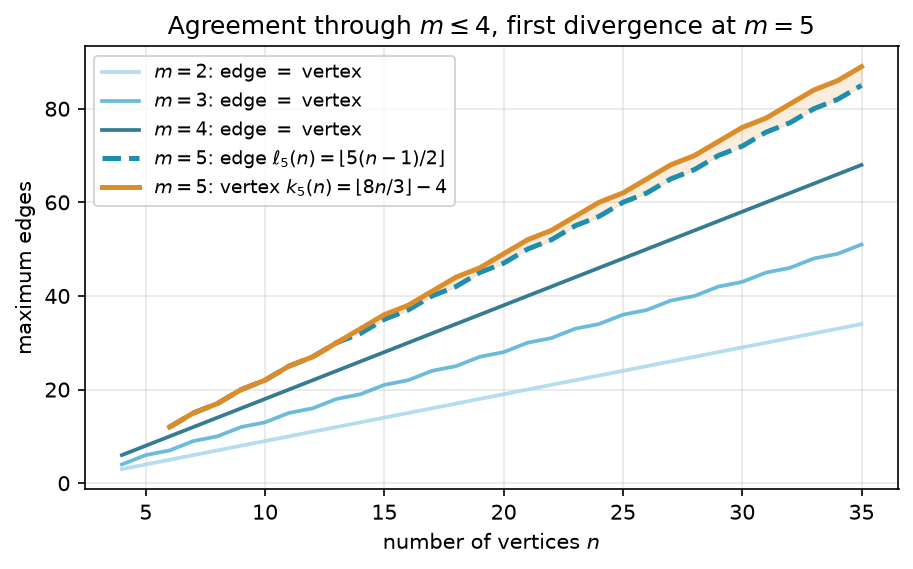
\includegraphics[width=\textwidth]{figures/edge_vertex_divergence.png}
    \caption{The edge and vertex extremal functions for $m = 2, 3, 4$ (blue shades, single curve per $m$ since they agree) and $m = 5$ (dashed blue for edge, solid orange for vertex). The vertex function diverges from the edge function at $n = 14$ and grows faster thereafter.}
    \label{fig:divergence}
\end{figure}

\begin{construction}[Directed hub]\label{const:directed-hub}
For $n \ge m \ge 2$, take a hub $h$ and label the other $N = n-1$ vertices $0, \dots, N-1$. Add the $2N$ hub arcs $h \to i$ and $i \to h$, and on the non-hub vertices the $(m-2)N$ ring arcs $i \to i+j \bmod N$ for $j = 1, \dots, m-2$. The total is $m(n-1)$ arcs and every non-hub vertex has $d^+ = d^- = m-1$.
\end{construction}

Every ordered pair has a non-hub member, whose relevant degree is exactly $m-1$ and, since $n \ge m$, smaller than the hub's own $n-1$. That member is therefore the binding one and the degree bound gives $\lec^{\max} \le m-1$. At $m = 2$ the ring is empty and what remains is the \emph{bidirected star}, in which two spokes can only reach each other through the hub.

\begin{construction}[One-directional bipartite digraph]\label{const:bipartite}
Split the vertices into parts $A$ and $B$ of sizes $\floor{n/2}$ and $\ceil{n/2}$, and include every arc from $A$ to $B$ and none the other way. The total is $\floor{n^2/4}$ arcs.
\end{construction}

Nothing leaves $B$ and nothing enters $A$, so no route has a second step and every pair is joined by at most the one direct arc, giving $\lec^{\max} = 1$.

\begin{theorem}[Directed arc value at $m = 2$]\label{thm:dir-arc-m2-exact}
For simple digraphs,
\[
    \ell_2^{\mathrm{dir}}(n) = \max\!\left(2(n-1),\ \floorfrac{n^2}{4}\right).
\]
\end{theorem}

The two constructions give the lower bound, one branch each. The upper bound is an induction on $n$ (\Cref{app:proofs}): delete a vertex of minimum total degree, which carries at most the average number of arcs, and apply the bound to what remains. The base cases $n \le 7$ are left to exhaustive search rather than hand argument, and \Cref{ch:machine} is what runs them. The same induction never mentions the separation, so it survives the change to $\kap$ verbatim once the base cases are re-run.

\begin{theorem}[Directed vertex value at $m = 2$]\label{thm:dir-vertex-m2-exact}
For simple digraphs, $k_2^{\mathrm{dir}}(n) = \ell_2^{\mathrm{dir}}(n)$.
\end{theorem}

\begin{figure}[h]
\centering
\begin{tikzpicture}[>=Stealth, scale=1.0,
    smallleftvertex/.style={gvertex}, smallrightvertex/.style={gvsink},
    hubvertex/.style={gvhub}, leftvertex/.style={gvertex},
    arc/.style={gdir},
    carc/.style={gdir, vertexorange!80!black}]

  % --- left panel: the bidirected star at n = 7, hub plus six spokes = 12 arcs ---
  \begin{scope}[shift={(-5.4,1.0)}, scale=0.92]
    \node[hubvertex, minimum size=7mm] (h) at (0,0) {$h$};
    \foreach \i/\ang in {0/90, 1/150, 2/210, 3/270, 4/330, 5/30} {
      \node[leftvertex, minimum size=7mm] (v\i) at (\ang:2.2) {$\i$};
    }
    \foreach \i in {0,...,5} {
      \draw[arc] (h) to[bend left=13] (v\i);
      \draw[arc] (v\i) to[bend left=13] (h);
    }
  \end{scope}
  % --- right panel: B_{3,4} at n = 7, every A-to-B arc = 12 arcs ---
  \begin{scope}[on background layer]
    \node[draw=KULblauw1!25, fill=KULblauw1!6, rounded corners=10pt,
          fit={(0,-0.6) (0,2.6)}, inner sep=8pt, minimum width=12pt] {};
    \node[draw=vertexred!25, fill=vertexred!6, rounded corners=10pt,
          fit={(4,-0.6) (4,2.6)}, inner sep=8pt, minimum width=12pt] {};
  \end{scope}
  \foreach \i in {1,...,3} {
    \node[smallleftvertex]  (a\i) at (0, {2.0-1.0*(\i-1)}) {$a_{\i}$};
  }
  \foreach \j in {1,...,4} {
    \node[smallrightvertex] (b\j) at (4, {2.5-1.0*(\j-1)}) {$b_{\j}$};
  }
  \foreach \i in {1,...,3} {
    \foreach \j in {1,...,4} {
      \draw[arc] (a\i) -- (b\j);
    }
  }
  \node[font=\small] at (0,-1.3) {$A$};
  \node[font=\small] at (4,-1.3) {$B$};
\end{tikzpicture}
\caption{The two branches tie at $n=7$, where each holds $12$ arcs at $\lec^{\max}=1$. Left: the bidirected star, a hub joined to six spokes both ways, $2(n-1)=12$. Right: the one-directional complete bipartite digraph $B_{3,4}$, every arc from $A$ to $B$, $\floor{n^2/4}=12$.}
\label{fig:simple-digraph-m2}
\end{figure}

The hub construction leads for $n < 7$, the one-directional bipartite construction leads for $n > 7$ and the two tie at $n = 7$, where both reach $12$ arcs. 
They are shown side by side in \Cref{fig:simple-digraph-m2}.
Notice how the directed value is quadratic in $n$ for large $n$, while the undirected value is linear.
This is because digraphs can be lopsided in one direction without creating routes back. 

\begin{proposition}[Hypergraph edge bound]\label{prop:hyper-edge}
An $r$-uniform hypergraph on $n$ vertices with Berge edge-connectivity at most $m-1$ has at most $\floorfrac{(m-1)(n-1)}{r-1}$ hyperedges. A simple hypergraph attains the bound whenever $m - 1 \le \binom{n-2}{r-2}$, and a multihypergraph attains it whenever $(r-1) \mid n - 1$.
\end{proposition}

The proof, given in \Cref{app:proofs}, runs the multigraph argument through the hypergraph Gomory-Hu theorem (\Cref{thm:hyper-gomory-hu} applied to the hyperedge-cut function in place of the edge-cut function, counting each hyperedge with the at least $r-1$ tree cuts it crosses. 
The star hypertree (\Cref{fig:hyper-star}) attains the $m = 2$ case, a hub joined to disjoint blocks of $r-1$ vertices, with Berge connectivity one everywhere and $\floor{(n-1)/(r-1)}$ hyperedges, exactly as a tree attained the multigraph bound. 
One genuine surprise is worth recording here: for $r \ge 3$ the bound is attained by \emph{simple} hypergraphs, with no repeated hyperedge, whenever $m-1\le\binom{n-2}{r-2}$ (\Cref{thm:simple-hyper-edge}). 
In the non-hypergraph case simplicity is exactly what separates Mader's $\floor{m(n-1)/2}$ from the multigraph value $(m-1)(n-1)$. 
One edge size higher, they are equal.

\begin{figure}[h]
\centering
\begin{tikzpicture}[scale=1.0,
   stn/.style={metrostop, minimum size=6mm},
   hub/.style={metrostop, minimum size=8.5mm, draw=vertexorange!90!black,
               fill=vertexorange!45, line width=1.4pt}]
  \coordinate (h) at (0,0);
  % two horizontal rows of four stations, the hub centred between them
  \coordinate (i1) at (-0.95, 1.3);  \coordinate (o1) at (-2.65, 1.3);
  \coordinate (i2) at ( 0.95, 1.3);  \coordinate (o2) at ( 2.65, 1.3);
  \coordinate (i3) at (-0.95,-1.3);  \coordinate (o3) at (-2.65,-1.3);
  \coordinate (i4) at ( 0.95,-1.3);  \coordinate (o4) at ( 2.65,-1.3);
  \begin{scope}[on background layer]
    % each hyperedge is one metro line: hub --(diagonal)-- inner --(horizontal)-- outer
    \draw[metro, metroA] (h) -- (i1) -- (o1);
    \draw[metro, metroB] (h) -- (i2) -- (o2);
    \draw[metro, metroC] (h) -- (i3) -- (o3);
    \draw[metro, metroD] (h) -- (i4) -- (o4);
  \end{scope}
  \foreach \p in {i1,o1,i2,o2,i3,o3,i4,o4} {\node[stn] at (\p) {};}
  \node[hub] at (h) {$h$};
\end{tikzpicture}
\caption{The $r=3$, $n=9$ star hypertree: four hyperedges meet only at the hub $h$, attaining $\floor{(n-1)/(r-1)}=4$ with Berge connectivity one.}
\label{fig:hyper-star}
\end{figure}

\begin{theorem}[Hypergraph vertex value at $m = 2$]\label{thm:hyper-vertex-m2}
For $r \ge 2$ and $n \ge 1$, the maximum number of hyperedges of an
$r$-uniform multihypergraph on $n$ vertices with $\kap^{\max} \le 1$ is
\[
    k_2^{(r)}(n) \;=\; \floorfrac{n-1}{r-1},
\]
attained by the star hypertree of \Cref{fig:hyper-star}. In particular
$k_2^{(r)}(n) = \ell_2^{(r)}(n)$: the vertex and edge problems agree at $m = 2$
for every uniformity, and repeated hyperedges never help.
\end{theorem}

\begin{theorem}[Hypergraph vertex value at $m = 3$]\label{thm:hyper-vertex-m3}
For $r \ge 2$, every $r$-uniform multihypergraph on $n$ vertices with
$\kap^{\max} \le 2$ has at most $\floorfrac{2(n-1)}{r-1}$ hyperedges. For
$r \ge 3$ with $2 \le \binom{n-2}{r-2}$ the bound is attained by a simple
hypergraph, so
\[
    k_3^{(r)}(n) \;=\; \floorfrac{2(n-1)}{r-1} \;=\; \ell_3^{(r)}(n).
\]
\end{theorem}

The first falls out once Berge routes are read as ordinary paths in the incidence graph, where the ceiling $\kap^{\max} \le 1$ says exactly that the incidence graph is a forest. 
The second is the harder one and carries the genuinely new tool: a rank bound for graphs in which one side of a partition must stay below local $3$-connectivity, proved by way of Tutte's triconnected decomposition, which the incidence translation then turns back into the hypergraph statement. 
At $m \ge 4$ that route stops for want of a $4$-connectivity analogue of the decomposition, and the value is open.
The proposition counts hyperedges, but it does not say how to \emph{measure} the Berge connectivity of a hypergraph we are handed and that measurement is the genuinely new part. 
The metro picture shows why. 
An ordinary edge is a one-stop link between a single pair, so policing edge-disjointness means watching each pair on its own. 
A hyperedge is a whole line: it stops at all $r$ of its vertices and so touches $\binom{r}{2}$ pairs at once, yet like a line that can run only one train at a time it may serve only one route. 
When several routes want to board the same line at different stations, the checker must wave exactly one through and turn the rest away and it must do this for every line simultaneously. 
That bookkeeping is the one new piece of machinery the next chapter builds and it is why the hypergraph rejoins the family only once the checker is in place.


\section{Conjectured bounds}

\begin{conjecture}\label{conj:dir-arc}
For simple digraphs and all $n \ge m \ge 2$,
\[
    \ell_m^{\mathrm{dir}}(n) = \max\!\left(m(n-1),\ \floorfrac{(n+m-2)^2}{4}\right).
\]
\end{conjecture}

At $m = 2$ this is \Cref{thm:dir-arc-m2-exact}. The first branch is the directed hub. The second is the bipartite digraph with one extra layer inside its larger part.

\begin{construction}[Augmented bipartite digraph]\label{const:augmented-bipartite}
For $n \ge m \ge 2$, set $|B| = \ceil{(n+m-2)/2}$ and $|A| = n - |B|$, include every arc from $A$ to $B$, and inside $B$ give each $b_j$ the $m-2$ in-arcs from its cyclic predecessors $b_{j-1}, \dots, b_{j-(m-2)}$. The total is $\floor{(n+m-2)^2/4}$ arcs.
\end{construction}

The only in-arcs of a $b \in B$ that an $a \in A$ can reach are the direct arc $a \to b$ and the $m-2$ two-step detours through $b$'s in-neighbours inside $B$, so such a pair carries exactly $m-1$ routes and no more, while pairs inside $B$ are held down by the in-degree $m-2$ and pairs from $B$ to $A$ or inside $A$ have no routes at all.

At $m = 3$, $n = 10$ this is the digraph that refutes the natural first guess $\max(m(n-1), \floor{n^2/4})$. Its $25$ arcs from $A$ to $B$ carry a five-cycle inside $B$, giving every $b_j$ one extra in-arc, so each pair $a_i, b_j$ has the direct arc and one detour and $\lec^{\max} = 2$. That is $30$ arcs against the guess of $27$, and the correction is exactly the shift of the partition towards $B$.

For fixed $m \ge 3$ the matching upper bound is open, though not entirely: \Cref{thm:dir-arc-linear-error} proves unconditionally that the value is $n^2/4 + \Theta_m(n)$, so what the conjecture still claims beyond what is known is the coefficient of the linear term rather than the shape of the answer.








% move all of this to the appendix. 
% \begin{construction}[Directed hub]\label{const:directed-hub}
% For $n \ge m \ge 2$, take a hub vertex $h$ and label the remaining $N = n - 1$ vertices $0, 1, \dots, N-1$. Add the $2N$ hub arcs $h \to i$ and $i \to h$ for every $i$, and on the non-hub vertices add the circulant arcs $i \to i + j \pmod{N}$ for $j = 1, \dots, m-2$, the target label wrapping around past $N$ back to $0$ (that ring pattern is what \emph{circulant} means, and ``$\bmod\ N$'' is the wrap-around). Counting these gives $2N$ hub arcs (each of the $N$ spokes joined to $h$ in both directions) plus $(m-2)N$ circulant arcs ($m-2$ layers, one arc per spoke), so the total is $2N + (m-2)N = mN = m(n-1)$ arcs. Every non-hub vertex has $d^+ = d^- = 1 + (m-2) = m-1$. Every ordered pair $(u,v)$ has at least one non-hub member, and that member's relevant degree is exactly $m-1$, smaller than the hub's own degree $n-1$ since $n \ge m$, so it is always the binding one regardless of which of $u,v$ is the hub. The directed degree bound (\Cref{lem:degree-bound}, which says $\lec(u,v)\le\min(d^+(u),d^-(v))$, since a route out of $u$ must use one of $u$'s out-arcs and one of $v$'s in-arcs) therefore gives $\lec^{\max} \le m-1$.
% \end{construction}
% At $m = 2$ this construction is easiest to picture: the circulant layer is empty and what remains is the \emph{bidirected star} of \Cref{fig:bidirected-star}, a hub joined to each spoke by a matched pair of opposite arcs. Every spoke can reach every other only by going in to the hub and back out, two hops, so no pair is ever joined by two independent routes, and the arc total is exactly $2(n-1)$. For $m \ge 3$ not all $m(n-1)$ arcs can touch the hub, since a simple digraph has at most $2(n-1)$ arcs incident to one vertex: the surplus lives in the circulant layers among the spokes, tuned so that no degree exceeds the budget. The two constructions compete on different scales, linear against quadratic, and which one wins depends on $n$. At $m = 2$ the competition resolves exactly.

% % --- right panel: m = 3 (hub + one circulant layer among spokes) ---
%   \begin{scope}[shift={(3.2,0)}, scale=0.92]
%     \node[hubvertex, minimum size=7mm] (H) at (0,0) {$h$};
%     \foreach \i/\ang in {0/90, 1/150, 2/210, 3/270, 4/330} {
%       \node[leftvertex, minimum size=7mm] (u\i) at (\ang:2.2) {$\i$};
%     }
%     % hub arcs (blue, both directions)
%     \foreach \i in {0,...,4} {
%       \draw[arc] (H) to[bend left=13] (u\i);
%       \draw[arc] (u\i) to[bend left=13] (H);
%     }
%     % single circulant layer j=1: i -> (i+1) mod 5  (orange), bowed outward
%     \foreach \i/\j in {0/1, 1/2, 2/3, 3/4, 4/0} {
%       \draw[carc] (u\i) to[bend right=22] (u\j);
%     }
%     \node[font=\small, text=black!70] at (0,-3.0) {$m=3$, $n=6$: $m(n{-}1)=15$ arcs};
%   \end{scope}
% \paragraph{Idea of the upper bound at $m = 2$.} Which of the two branches of $M(n) = \max(2(n-1), \floor{n^2/4})$ leads is pure arithmetic: $2(n-1) \ge \floor{n^2/4}$ precisely for $n \le 7$, with equality at $n = 7$, where both give $12$. So $M$ follows the bidirected star up to the crossover and the bipartite digraph past it, and $n = 7$ is the single size at which the two constructions tie. That no digraph beats $M(n)$ is an induction on $n$, carried out in \Cref{app:proofs}. Delete a vertex of \emph{minimum} total degree. Two facts about that deletion meet. The degrees sum to twice the arc count, so the deleted vertex carries at most the average $2a/n$ arcs, and what remains still respects the ceiling, so the inductive bound applies to it. Feeding both into the split of the arc count leaves a copy of $a$ on each side, and gathering them yields $a \le \tfrac{n}{n-2}\floor{(n-1)^2/4}$, which a parity check shows never exceeds $\floor{n^2/4}$ once $n \ge 8$. Nothing in the argument is deep. It is a careful walk through two parity regimes, with the base cases $n \le 7$ settled by exhaustive computer search rather than by hand. That experience of a correct but long and almost entirely mechanical case-check is exactly what motivates the chapters that follow. One genuinely wants to hand the case-checking to a machine.

% The vertex-disjoint version of the same question has the same answer at $m = 2$, but it is worth being careful about why, because Whitney's inequality is easy to read backwards here. Since $\kap \le \lec$ pairwise, a digraph that respects the arc ceiling automatically respects the vertex one, so the vertex-feasible family \emph{contains} the arc-feasible one and is in general strictly larger. The free consequence therefore runs one way only: the two constructions above keep $\kap^{\max} = 1$ as readily as $\lec^{\max} = 1$, which makes them lower bounds for the vertex problem too. No upper bound comes with them. What settles the vertex value is that the same induction goes through unchanged, because deleting a vertex lowers $\kap^{\max}$ for exactly the reason it lowers $\lec^{\max}$, and because the base cases $n \le 7$ were re-run under the stricter separation and returned the same six numbers. \Cref{app:proofs} gives both halves, and \Cref{rem:whitney-direction} there spells out the direction trap in full.


% \subsection{The failure of direct proof for \texorpdfstring{$m \ge 3$}{m >= 3}}
% For $m \ge 3$ the induction no longer closes, and the natural guess is wrong. The natural initial conjecture was that the two constructions above continued to be the whole story, giving $\max(m(n-1), \floor{n^2/4})$. A single graph on ten vertices refutes it.

% \begin{remark}[A thirty-arc counterexample]\label{rem:counterexample-m3}
% Take $A = \{a_1, \dots, a_5\}$ and $B = \{b_1, \dots, b_5\}$ with all $25$ arcs from $A$ to $B$, and add a directed five-cycle $b_1 \to b_2 \to b_3 \to b_4 \to b_5 \to b_1$ inside $B$. This digraph has $30$ arcs. Every vertex of $B$ has exactly one extra in-arc from inside $B$, so two arc-disjoint routes from $a_i$ to $b_j$ exist: the direct arc $a_i \to b_j$, and the detour $a_i \to b_{j-1} \to b_j$ using the 5-cycle predecessor of $b_j$ (indices mod 5). For the matching upper bound, the only in-arcs of $b_j$ reachable on a path from $a_i$ are the direct arc $a_i \to b_j$ and the cycle arc $b_{j-1} \to b_j$. Removing both disconnects $a_i$ from $b_j$, while neither alone does, so the minimum cut has size 2. Hence $\lec(a_i, b_j) = 2$. Routes between two vertices of $B$ never leave $B$ and give $\lec(b_i, b_j) = 1$. Hence $\lec^{\max} = 2$, so the graph is feasible at $m = 3$, yet $30 > \max(3 \cdot 9,\ 25) = 27$.
% \end{remark}

% \Cref{fig:augmented-bipartite} draws this thirty-arc digraph and traces the mechanism. The twenty-five faint arcs are the complete one-directional bipartite layer from $A$ to $B$, the construction we already understand. On top of them the orange five-cycle gives each vertex of $B$ a single extra in-arc from inside $B$. That one extra arc is exactly what doubles the connectivity. For the marked pair $a_1, b_2$ the two heavy routes show how: the blue arc is the direct hop $a_1 \to b_2$, and the green path $a_1 \to b_1 \to b_2$ borrows the cycle arc $b_1 \to b_2$ for its second step. The two share no arc, so $\lec(a_1, b_2) = 2$, and the same pair of routes exists for every $a_i, b_j$. Five extra arcs lift the whole digraph from one independent route per pair to two, and the thirty arcs overshoot the old prediction of twenty-seven.

% \begin{figure}[ht]
% \centering
% \begin{tikzpicture}[>=Stealth, scale=1.05,
%     smallleftvertex/.style={gvertex}, smallrightvertex/.style={gvsink},
%     bgarc/.style={gdirfaint},
%     directarc/.style={grBd, KULblauw1},
%     detourarc/.style={grBd, vertexgreen!75!black},
%     cycarc/.style={-{Stealth[length=1.8mm]}, line width=1.2pt, vertexorange!90!black, line cap=round}]
%   \foreach \i in {1,...,5} {
%     \node[smallleftvertex]  (a\i) at (0, {2.4-1.05*(\i-1)}) {$a_{\i}$};
%   }
%   \foreach \i in {1,...,5} {
%     \node[smallrightvertex] (b\i) at (4.0, {2.4-1.05*(\i-1)}) {$b_{\i}$};
%   }
%   % faint complete bipartite background (all 25 arcs)
%   \foreach \i in {1,...,5} {
%     \foreach \j in {1,...,5} {
%       \draw[bgarc] (a\i) -- (b\j);
%     }
%   }
%   % directed 5-cycle inside B, on the right
%   \foreach \i/\j in {1/2,2/3,3/4,4/5} {
%     \draw[cycarc] (b\i) to[bend left=58] (b\j);
%   }
%   \draw[cycarc] (b5) to[bend left=30] (b1);
%   % highlight the two arc-disjoint routes a1 -> b2 :
%   %  direct a1 -> b2 ;  detour a1 -> b1 -> b2 through the cycle arc
%   \draw[directarc] (a1) -- (b2);
%   \draw[detourarc] (a1) -- (b1);
%   \draw[detourarc] (b1) to[bend left=58] (b2);
%   \node[font=\small] at (0,-3.3) {part $A$};
%   \node[font=\small] at (4.0,-3.3) {part $B$};
% \end{tikzpicture}
% \caption{The thirty-arc counterexample at $m=3$, $n=10$: $25$ arcs run from $A$ to $B$ and a directed $5$-cycle lies inside $B$. The highlighted direct route and detour show the binding value $\lec^{\max}=2$.}
% \label{fig:augmented-bipartite}
% \end{figure}

% The counterexample generalises: the five-cycle gave every vertex of $B$ exactly one extra in-arc from inside $B$, and the budget for such arcs is $m - 2$ per vertex, not one. \Cref{fig:augmented-bipartite} is the instance $m = 3$, where that budget is one and a single cycle suffices. For larger $m$ each $b_j$ collects $m - 2$ cyclic predecessors and the same picture acquires more concentric chords inside $B$.

% \begin{construction}[Augmented bipartite digraph]\label{const:augmented-bipartite}
% For $m \ge 2$ and $n \ge m$, set $|B| = \ceil{(n+m-2)/2}$ and $|A| = n - |B| = \floor{(n-m+2)/2}$, include every arc from $A$ to $B$, and inside $B$ give each vertex $b_j$ the $m-2$ in-arcs from its cyclic predecessors $b_{j-1}, \dots, b_{j-(m-2)}$ (indices mod $|B|$). The total is $\floor{(n+m-2)^2/4}$ arcs.

% Its arc count is the product of the two halves of $n+m-2$, and its connectivity is verified in \Cref{app:proofs}. The point there is that the only in-arcs of a $b \in B$ that any $a \in A$ can reach are the direct arc $a \to b$ and the $m-2$ two-step detours through $b$'s in-neighbours inside $B$, so each such pair carries exactly $m-1$ arc-disjoint routes and no more, while pairs inside $B$ are held down by the in-degree $m-2$, and pairs from $B$ to $A$ or inside $A$ have no routes at all.

% At $m = 2$ the inside of $B$ is empty and the construction reduces to \Cref{const:bipartite}, with the balanced partition $(\floor{n/2}, \ceil{n/2})$. At $m = 3$ the formula gives $|B| = \ceil{(n+1)/2}$, which coincides with $\ceil{n/2}$ at odd $n$ but gives $|B| = n/2 + 1$ at even $n$. Both the balanced and the shifted partition achieve the same arc count $\floor{n^2/4} + \ceil{n/2}$ in this case, so the two are interchangeable at $m = 3$. The shift to a strictly larger $B$ is structurally significant only at $m \ge 4$, where the balanced partition is suboptimal. At $m = 3$, $n = 10$ it is the thirty-arc counterexample of \Cref{rem:counterexample-m3}, drawn in \Cref{fig:augmented-bipartite} (using the equivalent balanced partition $|A| = |B| = 5$).
% \end{construction}

% The two rival shapes invite a political picture. The hub is a single king through whom all traffic must pass, cheap to build but limited by the one throne. The bipartite family is a flat cabinet of ministers, each handling its own dossier with no central seat, and it scales quadratically. Which arrangement packs more arcs under the ceiling depends on $n$, and for $m \ge 3$ the cabinet overtakes the king once $n$ is large. This is the corrected shape, and it leads to the standing conjecture for the directed arc problem.



% The hypothesis $n \ge m$ is the one both constructions already carry, and it is needed for the same reason as in \Cref{thm:leonard}: below it the complete digraph is feasible and the answer is the trivial $n(n-1)$, which the formula exceeds. At $n = 3$, $m = 4$ the formula gives $8$ where three vertices carry only $6$ arcs. The exhaustive search confirms the value is $6$ there.

% For $m = 2$ this is \Cref{thm:dir-arc-m2-exact}. For $m = 3$ the formula $\floor{(n+1)^2/4}$ equals $\floor{n^2/4} + \ceil{n/2}$, so the conjecture reduces to the previous formula for $m = 2$ and $m = 3$. For $m = 3$, $n = 10$ the second branch gives $\floor{121/4} = 30$, matching \Cref{rem:counterexample-m3}. For $m \ge 4$ the new formula and the old balanced-partition count $\floor{n^2/4} + (m-2)\ceil{n/2}$ no longer agree. The quadratic branches already differ, and at $m = 4$ the new one is larger by exactly one at every even $n$. At small $n$, though, the hub term $m(n-1)$ dominates both branches and hides that difference. The full conjectured value therefore first overtakes the old one only at $n = 12$, for $m = 4$. The construction of \Cref{const:augmented-bipartite} with the shifted partition witnesses the difference. The lower bound holds for all $m$, witnessed by \Cref{const:directed-hub} on the first branch and \Cref{const:augmented-bipartite} on the second. For fixed $m\ge3$, the matching upper bound is open, though not entirely: \Cref{thm:dir-arc-linear-error} proves unconditionally that the value is $n^2/4 + \Theta_m(n)$, so what the conjecture still claims beyond what is known is the coefficient of that linear term rather than the shape of the answer. \Cref{ch:synthesis} returns to it with what structural progress the machine and the hand can jointly supply.

% \section{The hypergraph variant}
% The third model deserves its own short treatment, not because its base case is hard but because it is the one variant whose objects are stored and manipulated differently from all the rest, and it is worth meeting that difference now rather than at the moment of computation. A hypergraph keeps no multiplicity matrix, only the list of its hyperedges, each a set of $r$ vertices. We fix the edge size $r$, following the extremal literature, for a structural reason: under a connectivity ceiling a small edge is always at least as efficient per route as a large one, so a hypergraph free to mix sizes would maximise its edge count by using pairs only, and the question would collapse back to the graph case. Fixing $r$ is what makes the hypergraph question a new question.

% The route between two vertices is a \emph{Berge path}, which alternates vertices and hyperedges so that each consecutive pair of vertices lies in the hyperedge listed between them, and two such routes are edge-disjoint when they share no hyperedge. Concretely, in a three-uniform hypergraph a route from $u$ to $w$ might be the single step $u, \{u, x, w\}, w$ that crosses one hyperedge, or a longer alternation $u, \{u, x, y\}, y, \{y, z, w\}, w$ that switches hyperedge at the intermediate vertex $y$.

% With routes redefined this way the same Gomory--Hu machinery that proved the multigraph value carries over, and the base case has the same linear shape. The picture to keep in mind is a metro map: each hyperedge is a line, and a route from one vertex to another rides a line and changes to another line at a station the two share.

% A single hyperedge may serve only one route, so two Berge routes that share no hyperedge are edge-disjoint, the hypergraph counterpart of two edge-disjoint paths in a graph. In the metro picture, two hyperedges that share several vertices are distinct lines calling at several of the same stations, as in \Cref{fig:four-models}. Two routes are hyperedge-disjoint exactly when they never ride the same line.

% This is one of several inequivalent notions of hypergraph connectivity, and the choice matters, so it is worth saying which one is meant. Dewar, Pike and Proos \cite{DewarPikeProos18} survey the competing definitions and how they separate, and Berge routes with hyperedge-disjointness are the notion used throughout here, matching Berge's own \cite{Berge89}. The dual cut side is the hyperedge cut, whose minimisation is studied algorithmically by Chekuri and Xu \cite{ChekuriXu17}, and it is exactly the quantity the checker of \Cref{ch:machine} computes and the hypergraph Gomory--Hu tree of \Cref{thm:hyper-gomory-hu} organises.

% The separation axis needs its own definition here, and it is worth fixing now because the natural guess is not the one this thesis uses. Two Berge routes are called \emph{internally disjoint} when they share neither an intermediate vertex nor a hyperedge. Both halves are required. Demanding only that the routes avoid each other's intermediate stations would let two routes ride the same line, and a line that can run only one train at a time cannot serve two routes at once, so the resulting count would not correspond to anything the metro map can carry. Requiring both is also what makes the vertex measure the exact analogue of the graph one under the translation of \Cref{app:proofs}, where a hypergraph becomes its incidence graph, each hyperedge becomes a node, and internally disjoint routes become internally disjoint paths in the ordinary sense. It has the pleasant side effect that Whitney's inequality survives the move to hypergraphs by definition, since an internally disjoint family is in particular hyperedge-disjoint. Write $\kap_\HH(u,v)$ for the largest such family and $\kap^{\max}_\HH$ for its maximum over pairs.


% The edge bound is the easy half of the hypergraph story. The vertex separation is where this thesis has something new to say, and its two statements are worth having in front of the reader before the machinery that establishes them.

% all of this seems boring, i'd prefer you take what is needed to be mentioned: what parts of the implementation i actually should refer to, but that belongs in the next chapter. 
% \section{Where this work sits}
% %seems repetitive and not needed, 
% % It is worth pausing, before the machine, to place the question and the method against the two traditions they descend from: the extremal graph theory that posed the problem and the computational mathematics that will help settle it.

% % The mathematical lineage is the older of the two. The problem belongs to the family of extremal connectivity questions opened by Bollob\'{a}s and Erd\H{o}s, who asked how dense a graph can be while every pair of vertices stays below a fixed connectivity \cite{BollobasErdos62}, logged today as Erd\H{o}s Problem 915 \cite{ErdosProblems}. Mader's theorem \cite{Mader73} closed the simple undirected edge case with the clean floor $\floor{m(n-1)/2}$ recalled in \Cref{thm:mader}, and it is the floor every variant in this thesis is measured against. The vertex-disjoint branch has a longer and rougher history. Leonard \cite{Leonard72b} showed that the edge and vertex problems coincide through $m \le 4$, and S\o{}rensen and Thomassen \cite{SorensenThomassen74} found the first divergence at $m = 5$, where $k_5(n) = \floor{8n/3} - 4$ for every $n \ge 6$ except $n = 7$ and $n = 12$ (whose values are $15$ and $27$). Past that point the exact values $k_m(n)$ remain unknown. What is known there is one negative and one bound: the original conjecture of Bollob\'{a}s and Erd\H{o}s is false for every $m \ge 6$ \cite{Mader73}, and a general lower bound is available \cite{SorensenThomassen74}. That gap between a settled edge case and a stalled vertex case is exactly the terrain \Cref{ch:basecases} has been mapping, and the directed and hypergraph axes extend it further. To this particular lineage, the undirected vertex problem, the thesis adds no new closed form. It does add exact formulas and asymptotic results on the directed and hypergraph axes.

% The computational tradition this thesis's pipeline belongs to is the practice of settling combinatorial questions by machine in a way a human can audit, and it splits into a few schools worth contrasting with the certify-then-prove loop built next. The oldest is \emph{exhaustive generation}: enumerate every object of a given size up to isomorphism and check each one. McKay and Piperno's \texttt{nauty}/\texttt{geng} toolkit \cite{McKayPiperno14} is the standard engine for this, and its flagship results include exact small Ramsey numbers such as $R(4,5) = 25$ \cite{McKayRadziszowski95}. The enumeration of \Cref{ch:certify} is the same idea, run on the twelve variants of Problem 915. The second school is \emph{SAT-assisted proof}, in which a question is encoded in propositional logic and a solver emits a machine-checkable certificate. Two results are the canonical examples of certified solver output at scale: Heule, Kullmann and Marek's resolution of the Boolean Pythagorean triples problem \cite{HeuleKullmannMarek16}, whose verified proof runs to some two hundred terabytes, and Heule's determination of Schur number five \cite{Heule18}. The third is \emph{flag algebras}, Razborov's framework \cite{Razborov07} that converts asymptotic extremal bounds into semidefinite-programming certificates, the dominant tool for density problems in the large-$n$ limit. Closest of all to the method here is the fourth, \emph{certification by linear and integer programming} (LP/ILP). A feasibility or optimality argument over the rationals or integers is written as a linear program, meaning an optimisation whose constraints are all linear. Such a solve can in principle be accompanied by primal and dual data that a separate checker verifies. The cut-counting optimisation of \Cref{ch:certify} records the solver's status and an integral primal witness, but does not emit that independently replayable certificate. \Cref{sec:certification-standard} states the evidential standard used here.

% Against that backdrop, what is distinctive here is consolidation rather than a new solver. A single program measures connectivity exactly across all twelve problem variants through one common interface, using a matrix representation for graphs and a separate compact representation for hypergraphs, so search and certification share one codebase rather than living in separate tools. Its connectivity outputs and witnesses are exact integral objects. An optimiser's \texttt{OPTIMAL} status is recorded as machine evidence and is not presented as a formal certificate by itself. The general statements that use those finite values also have the independent hand proofs in \Cref{app:proofs}. Because the same program both hunts for dense graphs and checks the bounds they suggest, the discover and finite-verification steps are two modes of one loop. What makes the consolidation honest is that it never blurs three kinds of knowledge: a value can be \emph{proved} (by hand or exhaustive enumeration), \emph{solver-verified} at a finite size, or only \emph{conjectured} (witnessed by a dense graph with no matching upper bound). This trichotomy, named in \Cref{sec:trichotomy} and obeyed by the summary of \Cref{ch:synthesis}, is the through-line of everything that follows.

% \begin{computernote}
% We are now stuck in three different ways: a fifty-year-old open problem at $m \ge 6$ for vertices, a long proof we would rather not check by hand at $m = 2$ for arcs, and at $m \ge 3$ a conjecture of which only the leading behaviour can be proved. The base cases of the long induction were verified by exhaustive search. The thirty-arc counterexample was not: ten vertices put a blind sweep of digraphs far out of reach, so it was constructed and then confirmed pair by pair by the same exact checker. The next chapter builds a single program that models all of these cases at once, measures their connectivity exactly, and proves the small-case upper bounds outright.
% \end{computernote}


\chapter{Certifying and Discovering Bounds by Machine}
\label{ch:machine}\label{ch:certify}\label{ch:discover}

The previous chapter gave insight into the problem and some variants, but left most of the harder questions open.
This chapter will serve as a finite check of the results and conjectures by testing them on small graphs through brute-force enumeration.
It will also be the foundation of conjectures for the open cases, by discovering extremal graphs or at least sufficiently dense graphs.
Pattern recognition on the discovered values, or even a family of extremal graphs, then lets conjectures be made, although those statements are naive because they are based on small graphs only.
Larger graph spaces will be scoured by a heuristic, namely tabu search.
A guided search is needed there because only a small fraction of the search space is extremal: assigning edges at random gives a binomially distributed edge count, so almost every graph lands far from the cap.
The archive is the repository at \url{https://github.com/louisvandenbruwaene/thesis} and every file path quoted in this thesis is relative to it, or to a base directory named where the path is given, with the commands and the audit trail collected in \Cref{sec:transcripts}.
Below is a diagram of the program's architecture, showing how the modelled graphs are fed to the checker and how the results are used to either certify or discover bounds.
\begin{figure}[ht]
\centering
\spinediagram
\caption{A single model feeds the exact max-flow checker. Certification turns that measurement into finite upper bounds, while heuristic search uses it to discover lower bounds. The badge colours on the code cards match the boxes here.}
\label{fig:spine}
\end{figure}

\section{Modelling}
All non-hypergraphs are represented using one multiplicity matrix $\mu$: it is symmetric when undirected and binary when simple.
Hypergraphs are stored as (multi)sets of hyperedges, which are sets of vertices with a tail distinguished in the directed model.
\Cref{fig:matrix-rep} shows this encoding for a directed multigraph and hypergraph.
Matrix or tensor representations for hypergraphs are thus not recommended due to their size and sparsity.
All possible graphs of a given size will later be checked to see if they are extremal for the given size and connectivity restraint.
Matrices are iterated as a depth-first search with entries in $\{0,1\}$ for simple graphs and in $\{0,\ldots,m-1\}$ for multigraphs, and the diagonal is always zero.
Hypergraphs are implemented similarly from the ground up as there are no matrix tools for them.
Notice how depth-first search is memory-efficient.


\section{Measuring}
Given $n$ and $m$, walk through every graph on $n$ vertices, measure the largest
local connectivity $\lambda^{\max}$ or $\kap^{\max}$ of each with a max-flow computation and
keep the densest graph that stays at or below the cap $m - 1$.
If the enumeration cannot finish within the time limit, the best graph so far is returned.
It is therefore important to distinguish between the densest graph possible and the densest graph found.
A completed enumeration gives an exact extremal value. An unfinished enumeration gives only a lower bound.
In the vertex-disjoint and hypergraph cases the graph will be transformed before the flow can be measured.
This ensures that every variant shares the same integer max-flow engine no matter the implementation.
Thus the whole question reduces to a flow computation:
A \emph{maximum flow} asks how much can be pushed from one point to another through a network whose links each carry a limited capacity.
Menger's theorem (\Cref{thm:menger}) already turned $\lambda(u,v)$ into the number of edges/arcs in a minimum cut.
For a simple graph, $\lambda(u,v)$ is therefore also the capacity of a cut over a network with unit capacities.
For a multigraph, the parallel copies can be combined into one link whose capacity is their multiplicity $\mu(u,v)$.
In the directed case these capacities follow the direction of the arcs, while in the undirected case they are available in either direction.
The max-flow/min-cut theorem of Ford and Fulkerson \cite{FordFulkerson56} says that this smallest cut has exactly the value of a maximum flow.
So the route count we are after is just a maximum-flow value: measure the flow and you have measured the connectivity.

The routine that runs this flow and reports the route count is the connectivity \emph{checker}.
The program ships an optional compiled C helper that runs this same flow more efficiently.

\subsection{Transformations}
This max-flow computation is built for directed multigraphs (including simple digraphs) with edge-disjoint paths.
That is why the other variants will have to be transformed into such a flow network.
Undirected multigraphs have a natural identification with a directed multigraph, obtained by replacing every edge with a pair of arcs going in opposite directions.
To transform a multihypergraph, replace each distinct hyperedge with a helper gate,
an entry point and an exit point joined by a single arc whose capacity is the multiplicity of the hyperedge.
Every member of the hyperedge then flows into the entry and out of the exit at unlimited capacity,
so the one arc between them is the only bottleneck (\Cref{fig:hyper-gadget}).
A directed hyperedge is wired the same way, except that only its tail reaches the entry and only its heads leave the exit,
which is what forces a route to cross it from tail to head.
The directed hypergraph's flow network is just a restricted version of the undirected one.
Another representation for multihypergraphs is a separate gate with capacity one for each hyperedge.

The proposed hypergraph Menger argument (\Cref{thm:menger-hyper}) explains that the resulting maximum flow is exactly the Berge connectivity.
\Cref{fig:hyper-gadget-example} shows four gate-disjoint routes in a whole hypergraph.
For the vertex-disjoint hypergraph checker, only the ordinary vertices are split into unit-capacity gates. Each hyperedge retains its multiplicity-capacity gate.

Lastly, all vertex-disjoint versions can then be transformed into an identical edge-disjoint question by splitting
each vertex $v$ into an in-copy $v^{\mathrm{in}}$ and an out-copy $v^{\mathrm{out}}$ joined by a single unit-capacity arc (\Cref{fig:vertex-split}).
Every arc $u \to v$ of the digraph becomes $u^{\mathrm{out}} \to v^{\mathrm{in}}$ in the split network.
Routing through $v$ now consumes the one unit of capacity on its internal arc,
so two paths sharing $v$ as an intermediate vertex compete for that unit and cannot coexist in any maximum flow.
A max-flow from $u^{\mathrm{out}}$ to $v^{\mathrm{in}}$ in the split network therefore equals the number of internally vertex-disjoint $u$-$v$ paths in the original graph.
For a multigraph the arc carrying an adjacency keeps its full capacity
$\mu(u,v)$, and only the internal arc of a vertex is a unit. That is the
incidence convention of \Cref{sec:incidence-convention} written as a network:
parallel copies stay separate routes while the vertex they run through does not,
so the split network measures $K_m(n)$ and $K_m^{\mathrm{dir}}(n)$ rather than
the value of the underlying simple graph.
Notice how the undirected or hypergraph transformation is done beforehand and
the gates aren't split by this step.

\begin{figure}[htbp]
\centering
% Printed legibility: this picture holds two 8-unit panels side by side, so
% every extra centimetre of gap or of resize headroom is paid for twice over in
% label size. The gap is kept tight, the box is given the full text width, and
% the station and gate fonts are stepped up, which together lift the smallest
% label from about 5.4pt to roughly 9pt on paper.
\resizebox{\textwidth}{!}{%
\begin{tikzpicture}[scale=0.92, >=Stealth,
   metro/.append style={line width=3.0pt},
   metrostop/.append style={font=\small\bfseries, minimum size=6.6mm},
   faded/.style={metro, opacity=0.35, line width=2.2pt},
   flow/.style={line width=1.2pt, black!88, line cap=round,
                preaction={draw, line width=3.0pt, white}},
   gate/.style={circle, fill=white, draw=black!30, line width=0.6pt,
                inner sep=0.4pt, minimum size=13.5pt, font=\small}]
\def\stations{%
  \coordinate (Sa) at (0,0);  \coordinate (Sc) at (2,2);  \coordinate (Sd) at (6,2);
  \coordinate (Se) at (0,4);  \coordinate (Sj) at (8,4);  \coordinate (Sl) at (2,6);
  \coordinate (Sm) at (6,6);  \coordinate (Sn) at (0,8);}
% Every station carries its own letter, since the captions name hyperedges and
% routes by those letters.  The chosen pair also carries its role name, u or v,
% in blue just outside the station.
\def\drawstops{%
  \foreach \id/\lab in {Sa/a,Sc/c,Sd/d,Se/e,Sj/j,Sl/l,Sm/m,Sn/n}
     {\node[metrostop] at (\id) {$\lab$};}
  \node[font=\small\bfseries, text=KULblauw1] at ($(Se)+(-0.62,0.52)$) {$u$};
  \node[font=\small\bfseries, text=KULblauw1] at ($(Sm)+(0.62,0.52)$) {$v$};}
% --- panel (a): the hypergraph, every hyperedge vertex to vertex ---
\begin{scope}
  \stations
  \begin{scope}[on background layer]
    \draw[metro, metroA] (Se) -- (Sa);
    \draw[metro, metroA] (Sa) -- (Sd);
    \draw[metro, metroB] (Sn) -- (Sm);
    \draw[metro, metroB] (Sm) -- (Sj);
    \draw[metro, metroC] ($(Se)+(0.14,-0.14)$) -- ($(Sl)+(0.14,-0.14)$);
    \draw[metro, metroC] (Sl) -- (Sc);
    \draw[metro, metroD] (Se) -- (Sd);
    \draw[metro, metroD] (Sd) -- (Sm);
    \draw[metro, metroF] (Sn) -- (Se);
    \draw[metro, metroF] (Se) -- (Sl);
    \draw[metro, metroH] ($(Se)+(-0.14,0.14)$) -- ($(Sl)+(-0.14,0.14)$);
    \draw[metro, metroH] (Sl) -- (Sm);
    \draw[metro, metroG] (Sm) -- (Sc);
    \draw[metro, metroG] (Sc) -- (Sj);
    \draw[metro, metroE] (Sl) -- (Sd);
    \draw[metro, metroE] (Sd) -- (Sj);
  \end{scope}
  \drawstops
  \node[font=\small] at (4,-1.4) {(a)};
\end{scope}
% --- panel (b): the helper-point flow network for the pair u, v ---
\begin{scope}[xshift=9.6cm]
  \stations
  \coordinate (Helc) at (1,3);
  \coordinate (Hmcj) at (5,4);
  \coordinate (Hedm) at (3,3.7);
  \coordinate (Helm) at (1.6,6.7);
  \coordinate (Hnel) at (0.50,6.00);
  \coordinate (Hnmj) at (3.27,7.81);
  \begin{scope}[on background layer]
    \draw[faded, metroA] (Se) -- (Sa);
    \draw[faded, metroA] (Sa) -- (Sd);
    \draw[faded, metroB] (Sn) -- (Sm);
    \draw[faded, metroB] (Sm) -- (Sj);
    \draw[faded, metroC] ($(Se)+(0.14,-0.14)$) -- ($(Sl)+(0.14,-0.14)$);
    \draw[faded, metroC] (Sl) -- (Sc);
    \draw[faded, metroD] (Se) -- (Sd);
    \draw[faded, metroD] (Sd) -- (Sm);
    \draw[faded, metroF] (Sn) -- (Se);
    \draw[faded, metroF] (Se) -- (Sl);
    \draw[faded, metroH] ($(Se)+(-0.14,0.14)$) -- ($(Sl)+(-0.14,0.14)$);
    \draw[faded, metroH] (Sl) -- (Sm);
    \draw[faded, metroG] (Sm) -- (Sc);
    \draw[faded, metroG] (Sc) -- (Sj);
    \draw[faded, metroE] (Sl) -- (Sd);
    \draw[faded, metroE] (Sd) -- (Sj);
  \end{scope}
  \draw[flow] (Se) -- (Helc);
  \draw[flow] (Helc) -- (Sc);
  \draw[flow] (Sc) -- (Hmcj);
  \draw[flow] (Hmcj) -- (Sm);
  \draw[flow] (Se) -- (Hedm);
  \draw[flow] (Hedm) -- (Sm);
  \draw[flow] (Se) -- (Helm);
  \draw[flow] (Helm) -- (Sm);
  \draw[flow] (Se) -- (Hnel);
  \draw[flow] (Hnel) -- (Sn);
  \draw[flow] (Sn) -- (Hnmj);
  \draw[flow] (Hnmj) -- (Sm);
  % dotted leg from each gate to the hyperedge's unused third member
  \draw[densely dotted, line width=1pt, opacity=0.7, shorten >=3mm, metroC] (Helc) -- (Sl);
  \draw[densely dotted, line width=1pt, opacity=0.7, shorten >=3mm, metroG] (Hmcj) -- (Sj);
  \draw[densely dotted, line width=1pt, opacity=0.7, shorten >=3mm, metroD] (Hedm) -- (Sd);
  \draw[densely dotted, line width=1pt, opacity=0.7, shorten >=3mm, metroH] (Helm) -- (Sl);
  \draw[densely dotted, line width=1pt, opacity=0.7, shorten >=3mm, metroF] (Hnel) -- (Sl);
  \draw[densely dotted, line width=1pt, opacity=0.7, shorten >=3mm, metroB] (Hnmj) -- (Sj);
  \node[gate] at (Helc) {$h_{\textcolor{metroC}{\bullet}}$};
  \node[gate] at (Hmcj) {$h_{\textcolor{metroG}{\bullet}}$};
  \node[gate] at (Hedm) {$h_{\textcolor{metroD}{\bullet}}$};
  \node[gate] at (Helm) {$h_{\textcolor{metroH}{\bullet}}$};
  \node[gate] at (Hnel) {$h_{\textcolor{metroF}{\bullet}}$};
  \node[gate] at (Hnmj) {$h_{\textcolor{metroB}{\bullet}}$};
  \drawstops
  \node[font=\small] at (4,-1.4) {(b)};
\end{scope}
\end{tikzpicture}}
\caption[The helper-point network on a whole hypergraph]{An undirected $3$-uniform hypergraph and its gate network for $u,v$. The four black routes use distinct capacity-one gates (they are drawn as one point to reduce visual clutter), so the checker reads $\lec(u,v)=4$. A fifth would reuse a gate. The helper points connect to the hyperedge's third member by dotted lines.}
\label{fig:hyper-gadget-example}
\end{figure}

% Printed legibility: three panels across at 0.32\textwidth shrank each picture
% to roughly 0.58 of natural size and its labels to under 5pt. Stacking them
% one per row at 0.70\textwidth reverses that, drawing each slightly larger
% than natural instead.
\begin{figure}[ht]
\centering
\begin{subfigure}[b]{0.70\textwidth}
\centering
\resizebox{\linewidth}{!}{%
\begin{tikzpicture}[>=Stealth]
\node[vertex] (v) at (1.0, 0) {$v$};
\draw[->, edge] (0.0,  0.6) -- (v);
\draw[->, edge] (0.0, -0.6) -- (v);
\draw[->, edge] (v) -- (2.0,  0.6);
\draw[->, edge] (v) -- (2.0, -0.6);
\draw[->, very thick, color=KULblauw3b] (2.8, 0) -- (3.8, 0);
\node[smallvertex, minimum size=8mm] (vi) at (5.0, 0) {$v^{\mathrm{in}}$};
\node[smallvertex, minimum size=8mm] (vo) at (7.0, 0) {$v^{\mathrm{out}}$};
\draw[->, edge, color=KULblauw3b] (vi) -- node[above, font=\scriptsize]{capacity $1$} (vo);
\draw[->, edge] (4.0,  0.6) -- (vi);
\draw[->, edge] (4.0, -0.6) -- (vi);
\draw[->, edge] (vo) -- (8.0,  0.6);
\draw[->, edge] (vo) -- (8.0, -0.6);
\end{tikzpicture}}
\caption{Split each vertex $v$ into $v^{\mathrm{in}}$ and $v^{\mathrm{out}}$ joined by a unit-capacity arc to transform vertex-disjointness into edge-disjointness. Only this internal arc is a unit: an adjacency keeps capacity $\mu(u,v)$ and a hyperedge keeps its gate.}
\label{fig:vertex-split}
\end{subfigure}

\bigskip
\begin{subfigure}[b]{0.70\textwidth}
\centering
\resizebox{\linewidth}{!}{%
\begin{tikzpicture}[>=Stealth]
\coordinate (a) at (0.0, 0.0); \coordinate (b) at (1.0, 0.0); \coordinate (c) at (2.0, 0.0);
\begin{scope}[on background layer]\draw[metro, metroA] (a)--(b)--(c);\end{scope}
\node[smallvertex] at (a) {$a$}; \node[smallvertex] at (b) {$b$}; \node[smallvertex] at (c) {$c$};
\draw[->, very thick, color=KULblauw3b] (2.85, 0.0) -- (3.95, 0.0);
\begin{scope}[xshift=4.6cm]
% members in a column, gate pair beside them: every member sends one uncapped
% arc into e^- and receives one uncapped arc out of e^+.
\node[smallvertex] (a2) at (0.0,  1.30) {$a$};
\node[smallvertex] (b2) at (0.0,  0.00) {$b$};
\node[smallvertex] (c2) at (0.0, -1.30) {$c$};
\node[hnode, fill=metroA!70, minimum size=15pt] (em) at (2.05,  0.62) {$e^-$};
\node[hnode, fill=metroA!70, minimum size=15pt] (ep) at (2.05, -0.62) {$e^+$};
% into the gate
\draw[gdirfaint] (a2) to[bend left=8]  node[above, font=\scriptsize, text=black!55, pos=0.55]{$\infty$} (em);
\draw[gdirfaint] (b2) to[bend left=10] (em);
\draw[gdirfaint] (c2) to[bend left=22] (em);
% out of the gate
\draw[gdirfaint] (ep) to[bend left=22] (a2);
\draw[gdirfaint] (ep) to[bend left=10] (b2);
\draw[gdirfaint] (ep) to[bend left=8]  node[below, font=\scriptsize, text=black!55, pos=0.45]{$\infty$} (c2);
% the one bottleneck
\draw[gdir, line width=1.6pt, color=KULblauw3b] (em) -- node[right, font=\scriptsize]{capacity $\mu$} (ep);
\end{scope}
\end{tikzpicture}}
\caption{Transform a hyperedge into a gate with capacity equal to the multiplicity of the hyperedge.}
\label{fig:hyper-gadget}
\end{subfigure}

\bigskip
\begin{subfigure}[b]{0.70\textwidth}
\centering
\resizebox{\linewidth}{!}{%
\begin{tikzpicture}[>=Stealth, gatearc/.style={gdir}]
\node[smallvertex] (a) at (0.0, 1.05) {$a$}; \node[smallvertex] (b) at (-0.85, -0.55) {$b$}; \node[smallvertex] (c) at (0.85, -0.55) {$c$};
\begin{scope}[on background layer]
  \draw[metro, metroB, -{Stealth[length=2.8mm]}, shorten >=2mm, shorten <=1.4mm] (a) -- (b);
  \draw[metro, metroB, -{Stealth[length=2.8mm]}, shorten >=2mm, shorten <=1.4mm] (a) -- (c);
\end{scope}
\draw[->, very thick, color=KULblauw3b] (2.4, 0.1) -- (3.5, 0.1);
\begin{scope}[xshift=5.4cm]
  \node[smallvertex] (a2) at (0.0, 1.55) {$a$};
  \node[hnode, fill=metroB!70, minimum size=15pt] (gm) at (0.0,  0.52) {$e^-$};
  \node[hnode, fill=metroB!70, minimum size=15pt] (gp) at (0.0, -0.62) {$e^+$};
  \node[smallvertex] (b2) at (-1.05, -1.55) {$b$}; \node[smallvertex] (c2) at (1.05, -1.55) {$c$};
  \draw[gdirfaint] (a2) -- node[right, font=\scriptsize, text=black!60]{$\infty$} (gm);
  \draw[gdir, line width=1.6pt, color=KULblauw3b] (gm) -- node[right, font=\scriptsize]{capacity $\mu$} (gp);
  \draw[gdirfaint] (gp) -- node[left, pos = 0.3, font=\scriptsize, text=black!60]{$\infty$} (b2);
  \draw[gdirfaint] (gp) -- node[right, pos = 0.3, font=\scriptsize, text=black!60]{$\infty$} (c2);
\end{scope}
\end{tikzpicture}}
\caption{The directed hyperedge is transformed into a gate with one tail and two heads. This gate has capacity equal to the multiplicity of the hyperedge and every route must enter at the tail and leave at a head.}
\label{fig:dir-hyper-gadget}
\end{subfigure}
\caption{The building blocks of the connectivity checker: vertex splitting, hyperedge gates and directed hyperedge gates.}
\label{fig:checker-gadgets}
\end{figure}

\section{Checking every graph of a fixed size}\label{sec:certification-standard}
The connectivity checker works on all variants but measures only one graph at a time.
To establish an exact value by enumeration, every feasible graph must either be checked or excluded by a sound pruning argument. This is one route to an upper bound. A mathematical theorem can establish it without enumeration.
A simple graph on $n$ vertices is a choice of $\mu(u,v) \in \{0,1\}$ on each off-diagonal entry, a multigraph a choice in $\{0,\dots,m-1\}$,
and a digraph varies every ordered pair rather than only the upper triangle.
A hypergraph is not a matrix at all, so it is enumerated over its own list: a subset of all $\binom{n}{r}$ possible vertex sets of size $r$.
In the directed model, the tail is specified with a pointer and the multihypergraphs have multiplicities for each hyperedge.
\Cref{fig:matrix-rep} shows how a directed multigraph and hypergraph are represented.
Using these representations for all graph variants means iteration traverses all possible representation states easily.
Walking those possibilities, measuring each candidate with the checker and keeping the densest feasible graph settles a bound exactly.
If the enumeration hits its deadline before finishing, the returned graph is labelled as a lower bound.
Completed enumerations establish the small cases reported in the audit. For directed multigraphs under arc separation, \code{solve(exhaustive=True)} instead evaluates the conjectured formula and returns a named witness, explicitly labelled as a lower bound. This branch supplies no enumeration markers in the figures. The specialised structural enumerators use that same conjectured formula for prefix pruning, so their completeness is conditional and they cannot independently prove it.

\begin{figure}[ht]
    \centering
    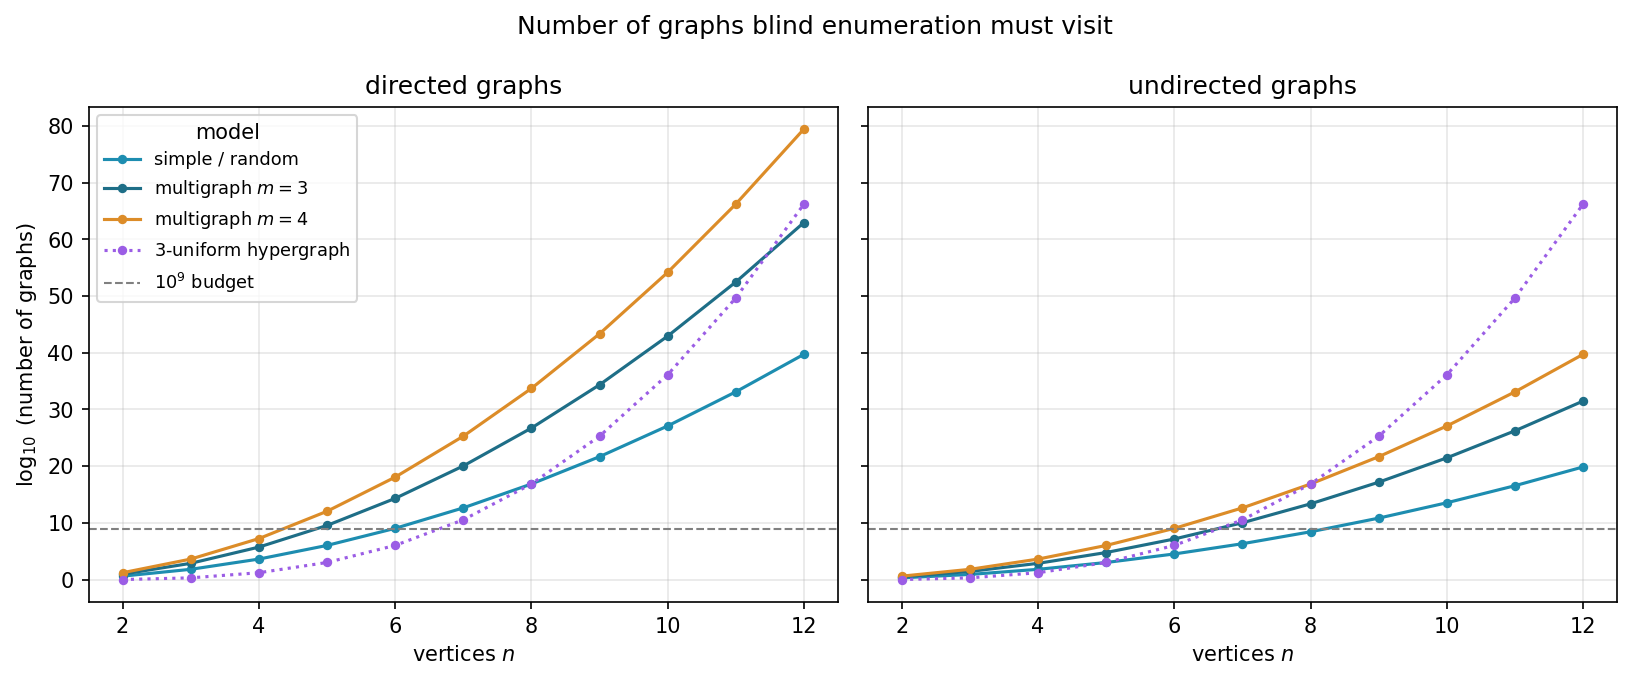
\includegraphics[width=\textwidth]{figures/complexity_growth.png}
    \caption{Candidate counts for blind enumeration on a logarithmic scale. Every model crosses the generous $10^9$ budget in single-digit order, and directed objects grow fastest because they have more independent entries to decide.}
    \label{fig:complexity}
\end{figure}

The vertex count dominates every other factor.
The candidate count has the form (values per entry)$^{\text{(number of entries)}}$.
For graphs, the number of entries grows quadratically with $n$.
For fixed-rank $r$-uniform hypergraphs, it grows as $\binom{n}{r}=\Theta(n^r)$.
The $r=3$ experiments plotted here therefore have cubic growth in the exponent.

Raising the connectivity budget enlarges the number of values available in each entry.
A simple graph has two states per entry, while a multigraph has more.
Adding direction instead increases the number of entries.
It decides both directions of a pair independently, turning two undirected states into four directed states.
Which change costs more depends on $m$ and on the model.
Directed hypergraphs are especially numerous because each hyperedge also requires a
choice of tail and heads.
These variants are particularly costly to enumerate, even where a conjecture predicts their leading term.
The separation, by contrast, does not change the enumeration: edge and vertex disjointness
start from the same candidate space, but use different feasibility tests. Their pruning and running times can therefore differ.

\begin{figure}[ht]
\centering
\begin{tikzpicture}[>=Stealth]
% ---- (a) digraph -> multiplicity matrix, diagonal highlighted, asymmetric ----
\node[vertex] (A) at (0,   0)   {$1$};
\node[vertex] (B) at (2.0, 0)   {$2$};
\node[vertex] (C) at (1.0, 1.7) {$3$};
\draw[arc] (A) to[bend left=15]  (B);
\draw[arc] (A) to[bend right=15] (B);
\draw[arc] (B) to[bend left=15]  (C);
\draw[arc] (C) to[bend left=15] (B);
\draw[arc] (A) -- (C);
\node[font=\small] at (1.0, -0.8) {directed multigraph $G$};
\node at (3.3, 0.55) {$\xrightarrow{\;\mu\;}$};
\node at (5.4, 0.55) {$\begin{pmatrix} {\color{vertexred}\mathbf 0} & 2 & 1 \\ 0 & {\color{vertexred}\mathbf 0} & 1 \\ 0 & 1 & {\color{vertexred}\mathbf 0} \end{pmatrix}$};
\node[font=\small] at (5.4, -0.8) {multiplicity matrix $\mu$};
\node[font=\scriptsize, vertexred] at (5.4, -1.3) {Diag($\mu$)$=0$ (no loops)};
% ---- (b) directed hypergraph -> list of hyperedges, tail 3 shared by both ----
\begin{scope}[yshift=-3.5cm]
  \coordinate (p1) at (0.0, 0.6);
  \coordinate (p2) at (0.0,-0.6);
  \coordinate (p3) at (1.1, 0.0);
  \coordinate (p4) at (2.2, 0.6);
  \coordinate (p5) at (2.2,-0.6);
  \begin{scope}[on background layer]
    \draw[metro, metroA, -{Stealth[length=2.6mm]}, shorten >=2mm, shorten <=1.4mm] (p3) -- (p1);
    \draw[metro, metroA, -{Stealth[length=2.6mm]}, shorten >=2mm, shorten <=1.4mm] (p3) -- (p2);
    \draw[metro, metroB, -{Stealth[length=2.6mm]}, shorten >=2mm, shorten <=1.4mm] (p3) -- (p4);
    \draw[metro, metroB, -{Stealth[length=2.6mm]}, shorten >=2mm, shorten <=1.4mm] (p3) -- (p5);
  \end{scope}
  \foreach \p/\lbl in {p1/1,p2/2,p3/3,p4/4,p5/5} {\node[smallvertex] at (\p) {$\lbl$};}
  \node[font=\small] at (1.1,-1.25) {directed hypergraph $H$};
  \node at (3.3, 0.0) {$\longrightarrow$};
  \node[font=\small, align=left] at (5.9, 0.0)
    {list of hyperedges:\\[3pt] $e_1: \{3\ |\ 1,2\}$\\[1pt] $e_2:\{3\ |\ 4,5\}$};
\end{scope}
\end{tikzpicture}
\caption{The two encodings for directed variants. The multiplicity matrix $\mu$ represents a digraph, with $\mu_{ij}$ arcs from $i$ to $j$. A list of hyperedges represents a directed hypergraph and records each tail separately. A multihypergraph repeats entries in that list. A tensor representation would require $n^r$ entries, almost all zero, and is therefore avoided.}
\label{fig:matrix-rep}
\end{figure}

The number of graphs the checker must visit grows as $2^{\binom{n}{2}}$ for simple undirected graphs and $2^{n(n-1)}$ for digraphs,
and capping multiplicities at $m-1$, so that each run ranges over the $m$ values $\{0,\dots,m-1\}$, raises the base from two to $m$,
giving $m^{\binom{n}{2}}$ undirected multigraphs and $m^{n(n-1)}$ directed ones.
The enumeration is exact wherever it finishes and it does so only for the smallest sizes.
\Cref{fig:complexity} measures exactly how fast the search space grows.

\subsection{Pruned search}
The enumeration step will skip whole families of hopeless graphs, via a pruned search.
The directed $m=2$ values are checked independently at every order through $n=7$, under both separations (\Cref{tab:basecase-search}).
\Cref{thm:dir-vertex-m2-exact,thm:dir-arc-m2-exact} propose all-order formulas whose upper-bound proofs depend on the unchecked reachability-skeleton argument. The sweep establishes only the listed finite cases.
Those orders lie just beyond the range where blind digraph enumeration is practical.
They can be reached by enumerating more cleverly.
Every variant offers a fixed list of edges its graphs are allowed to use,
whether those are pairs, ordered pairs, or oriented sets of $r$ vertices,
and a graph is a choice of how many copies each of them gets.
Rather than writing out whole choices one after another,
fix an order on that list and decide the edges one at a time,
leaving the undecided ones absent.
Each partly built graph then stands for the whole family of graphs agreeing with it so far,
and a pruning rule discards that entire family if it is deemed to bear no fruit.

Adding an edge never lowers connectivity because every existing family of disjoint routes survives (\Cref{prop:monotone}).
Every completion of a partly built graph only adds edges.
The partial graph is therefore a lower bound on the connectivity of every completion.
If it already breaks the cap, every completion does too.
The entire branch can then be abandoned.

A second pruning method starts with the edges already placed.
It then adds the largest possible contribution from the undecided edges: their number times the largest allowed multiplicity.
The resulting sum is an upper bound on every completion.
If this upper bound cannot beat the best feasible graph found so far, the branch is discarded without further exploration (\Cref{fig:prune}).
Only infeasible graphs and graphs that cannot beat the incumbent are ever discarded, so a run that finishes returns exactly the maximum the basic walk would have returned.

\begin{figure}[ht]
\centering
\begin{tikzpicture}[scale=1.0, >=Stealth,
   live/.style={gvertex, minimum size=5.5mm},
   dead/.style={gvsink, minimum size=5.5mm},
   bnd/.style={gvhub, minimum size=5.5mm},
   best/.style={gvertex, draw=vertexgreen!70!black, fill=vertexgreen!18, minimum size=5.5mm},
   br/.style={gline}]
  \node[live] (r) at (0,0) {};
  \node[live] (l) at (-2.2,-1.3) {};
  \node[live] (rr) at (2.2,-1.3) {};
  \draw[br] (r) -- node[above left, font=\scriptsize, pos=0.55]{add arc} (l);
  \draw[br] (r) -- node[above right, font=\scriptsize, pos=0.55]{skip arc} (rr);
  \node[best] (l1) at (-3.1,-2.7) {};
  \node[dead] (l2) at (-1.4,-2.7) {};
  \draw[br] (l)--(l1);
  \draw[line width=1pt, vertexred!60] (l)--(l2);
  \node[dead] (r1) at (1.3,-2.7) {};
  \node[bnd]  (r2) at (3.1,-2.7) {};
  \draw[line width=1pt, vertexred!60] (rr)--(r1);
  \draw[line width=1pt, vertexorange!70] (rr)--(r2);
  \node[font=\scriptsize, vertexgreen!50!black, align=center] at (-3.1,-3.5) {best\\feasible};
  \node[font=\scriptsize, vertexred, align=center] at (-1.4,-3.5) {infeasible\\(prune)};
  \node[font=\scriptsize, vertexred, align=center] at (1.3,-3.5) {infeasible\\(prune)};
  \node[font=\scriptsize, vertexorange!80!black, align=center] at (3.1,-3.5) {cannot beat\\best (prune)};
\end{tikzpicture}
\caption{Each level of the partially built graph fixes one adjacency. Infeasible partial graphs (red) and branches unable to beat the incumbent (orange) are discarded.}
\label{fig:prune}
\end{figure}

\subsection{Generating search}
Iterating over all possible graphs and measuring each one's connectivity repeats many isomorphic cases.
Another method, suggested by Prof.\ Jan Goedgebeur, instead generates all non-isomorphic graphs.
It uses the \texttt{geng} program from the \texttt{nauty} toolkit of McKay and Piperno \cite{McKayPiperno14}
to perform the difficult task of generating one representative of each isomorphism class.
The program is called as a subprocess, and its \texttt{graph6} output is decoded.
For a given $n$, \texttt{geng} produces all non-isomorphic \emph{undirected} graphs.
The program then treats each such graph as a support graph and assigns directed arc multiplicities to its edges.
Consequently, the search automatically inherits the support graph's isomorphism reduction.
For each support edge $\{u,v\}$, considered in a fixed order, it assigns the ordered pair
of multiplicities $\mu(u,v)$ and $\mu(v,u)$. Each lies between $0$ and $m-1$, and the two cannot both be zero because every support edge must represent at least one arc.
After each assignment, the checker evaluates the partially decorated multigraph.
If any pair already exceeds the allowed connectivity, that branch is stopped immediately:
adding more arcs cannot decrease connectivity. This is the same monotonicity-based pruning used in \Cref{fig:prune}.
Decorations that reach the target arc count are retained and converted to canonical form,
which ensures that each isomorphism class is reported only once.
Because different support graphs produce disjoint search spaces, they can be processed independently on separate processor cores.
The related orientation tools \texttt{directg} and \texttt{watercluster2} are not used.
Both allow edges in both directions, but they do not assign the repeated arc multiplicities used here \cite{NautyGuide29}. The custom decoration step also applies the connectivity pruning after each assignment.

\Cref{tab:generating-benchmark} records historical timings for three different single-core tasks. The distinction matters: they are not three equivalent ways of discovering an unknown optimum.
The blind sweep maximises the arc count over all matrix assignments.
The pruned depth-first search also maximises it, but starts with a supplied feasible construction as an incumbent.
The \texttt{geng} pipeline is given the already known extremal arc count and lists the feasible isomorphism classes at that target. Finding representatives there does not rule out a larger feasible count, so this last run does not prove the optimum independently.

The blind sweep is omitted after $n=4$, where $2^{n(n-1)}$ assignments already take $6.3$\,s.
Each additional vertex multiplies the assignment count by $2^{2n}$.
The estimated runtime is about an hour at $n=5$ and several weeks at $n=6$.
This is the growth shown in \Cref{fig:complexity}.

Below $n=5$, fixed overhead dominates the two remaining methods.
The main costs there are Python function calls and subprocess start-up.
Those timings do not give a meaningful comparison of search performance.
At $n=7$, the recorded pruned maximisation takes $1156.6$\,s and the supplied-target classification takes $17.0$\,s. Their different outputs and prior information prevent interpreting this ratio as a speed-up for proving an unknown optimum. The script gives the pruned search a $1800$-second stopping target. The blind and generated routines have no common time limit. These observations illustrate the cost of the respective tasks, not an equal-budget performance comparison.

\begin{table}[ht]
    \centering
    \small
    % Times measured on the author's machine, single core (geng parallel=False),
% directed simple digraphs, m=2. Generated classification is GIVEN the optimal
% target count and does not independently prove optimality. Blind sweep
% omitted past n=4, where 2^(n(n-1)) assignments already cost 6.3s. Each
% further vertex multiplies the assignment count by 2^(2n), and the per-
% assignment check grows too: the recorded n=3 to n=4 step cost about twice
% its count ratio. Both factors together put n=5 near an hour and n=6 at
% weeks. Reproduced by
% program/scripts/generating_search_benchmark.py against erdos915_unified.py.
\begin{tabular}{rrrrr}
\toprule
$n$ & supplied target & blind (s) & pruned (s) & classification (s) \\
\midrule
3 & 4  & 0.05 & 0.003 & 0.009 \\
4 & 6  & 6.3  & 0.008 & 0.008 \\
5 & 8  & --   & 0.22  & 0.039 \\
6 & 10 & --   & 14.5  & 0.73  \\
7 & 12 & --   & 1156.6 & 17.0 \\
\bottomrule
\end{tabular}

    \caption{Historical timings for different tasks: blind maximisation, construction-seeded pruned maximisation and \texttt{geng}-based classification at a supplied target. Only the first two independently bound the optimum from above. A dash means not attempted. These are separate runs from \Cref{tab:basecase-search}, whose recorded times differ. The table is not evidence of a like-for-like speed-up.}
    \label{tab:generating-benchmark}
\end{table}
\section{Proving every \texorpdfstring{$m$}{m} at once}

The search so far treats one pair $(n,m)$ at a time.
For a directed multigraph, scaling can instead check every threshold at a fixed $n$ in one pass.
It divides all multiplicities by $m-1$.
The formula in \Cref{thm:dir-multi-full} now supplies a lower-bound witness in \code{solve}. The cut formulation can provide a separate finite check, provided its optional cuts are valid independently of that conjecture.

Divide each multiplicity of a feasible directed multigraph $D$ by $m-1$.
The resulting weights satisfy $w(u,v)\in[0,1]$.
Every pairwise maximum flow is at most one.
Their total weight is the arc count of $D$ divided by $m-1$ (\Cref{fig:scaling-reduction}).
Let
\[
    M^{*}(n) = \max\Bigl\{\textstyle\sum_{u \ne v} w(u, v) : w(u,v) \in [0,1], \ \mathrm{maxflow}(s, t; w) \le 1 \ \text{for all } s \ne t\Bigr\}
\]
denote the largest total weight of such a matrix.
Scaling then gives
\[
    L_m^{\mathrm{dir}}(n) \;\le\; (m - 1)\, M^{*}(n)
    \qquad \text{for every } m \ge 2 .
\]

The reverse inequality needs a $\{0,1\}$ matrix of weight $M^{*}(n)$.
Multiplying such a matrix by $m-1$ preserves integer arc multiplicities.

On the linear branch, \Cref{const:dir-multi-lower} supplies the double star.
It has one hub joined bidirectionally to every other vertex and has $2(n-1)$ arcs.
For $n\le6$, this is the larger term of $M(n)$ and realises $M^{*}(n)$.
At the crossover $n=7$, the quadratic branch catches the linear one (\Cref{thm:dir-arc-m2-exact}).
It then overtakes it.
The relevant construction becomes the one-directional bipartite digraph from \Cref{const:dir-multi-lower}.
Thus no single shape witnesses $M^{*}(n)$ at every order.

What would generalise is integrality.
\Cref{cor:mstar-integral} proposes that some $\{0,1\}$ matrix always attains $M^{*}(n)$, and that this optimum equals $M(n)$.
An explicit construction gives attainment from below.
Clearing denominators from a rational optimum reduces the reverse inequality to \Cref{thm:dir-multi-full}, whose proposed proof is unchecked, so the identity below inherits that dependency.
Scaling the integral maximiser by $m-1$ gives the lower bound $(m-1)M^{*}(n)$.
The preceding scaling argument gives the matching upper bound unconditionally.
The finite optimisation is retained only as an independent check of the cases $n\le6$, and \Cref{sec:transcripts} records what it ran.
\[
    L_m^{\mathrm{dir}}(n) = (m - 1)\, M^{*}(n)
    \qquad \text{for every } m \ge 2 .
\]
\begin{figure}[ht]
\centering
\begin{tikzpicture}[>=Stealth, font=\small]
    % Left: integer multigraph (m=3), multiplicities in {0,1,2}
    \node[vertex] (A1) at (-4.2, 0)   {$A$};
    \node[vertex] (B1) at (-2.4, 1.1) {$B$};
    \node[vertex] (C1) at (-2.4,-1.1) {$C$};
    % A->B multiplicity 2: two parallel arcs
    \draw[->, arc] (A1) to[bend left=22]  node[above, font=\scriptsize]{$2$} (B1);
    \draw[->, arc] (A1) to[bend right=5]  (B1);
    % A->C multiplicity 1
    \draw[->, arc] (A1) -- node[below, font=\scriptsize]{$1$} (C1);
    % B->C multiplicity 0: absent (dotted, grayed out)
    \draw[->, arc, color=gray!50, dashed] (B1) -- node[right, font=\scriptsize, color=gray!60]{$0$} (C1);
    \node[above, font=\footnotesize\itshape] at (-3.3, 1.8) {multigraph ($m=3$)};

    % Scaling arrow
    \draw[->, very thick] (-1.2, 0) -- (1.2, 0);
    \node[above, font=\small] at (0, 0.1) {$\div\,(m-1)\;=\;\div\,2$};

    % Right: weight matrix, weights in [0,1]
    \node[vertex] (A2) at (2.4, 0)   {$A$};
    \node[vertex] (B2) at (4.2, 1.1) {$B$};
    \node[vertex] (C2) at (4.2,-1.1) {$C$};
    % A->B weight 1
    \draw[->, arc] (A2) -- node[above, font=\scriptsize]{$1$} (B2);
    % A->C weight 1/2
    \draw[->, arc] (A2) -- node[below, font=\scriptsize]{$\tfrac{1}{2}$} (C2);
    % B->C weight 0: absent
    \draw[->, arc, color=gray!50, dashed] (B2) -- node[right, font=\scriptsize, color=gray!60]{$0$} (C2);
    \node[above, font=\footnotesize\itshape] at (3.3, 1.8) {weight matrix ($M^*$)};
\end{tikzpicture}
\caption{Scaling at $m=3$: dividing multiplicities by $m-1=2$ turns the integer multigraph into a weight matrix with entries in $[0,1]$ and pairwise maximum flow at most one. Hence one $m$-free optimisation bounds every threshold.}
\label{fig:scaling-reduction}
\end{figure}

\section{The heuristic search}
So far, iterating all graphs of a fixed size that meet the connectivity constraint and counting their edges was a blind walk.
Apart from pruning, there is nothing that steers the walk towards better candidates because they all need to be checked anyway.
From a certain point onwards, that will become impossible due to the massive number of possible graphs.
The goal then becomes finding the densest possible graphs in such an efficient and guided way that they are
likely to be (almost) extremal.
The guide that pulls the walk towards a (local) maximum is called a heuristic.
To avoid getting stuck in a local maximum, a metaheuristic allows worsening moves to discover new optima.

For graph and digraph models represented by a multiplicity matrix, give each candidate one number: its energy
\[
    \Phi(G) = -|E(G)| + \Lambda \cdot \max\bigl(0,\ c^{\max}(G) - (m - 1)\bigr),
\]
which rewards edges or arcs and penalises any excess connectivity, where $c^{\max}(G)$ denotes $\lambda^{\max}(G)$ or $\kappa^{\max}(G)$, matching whichever separation the run measures.
The matrix search starts from the empty graph and changes one edge or arc multiplicity by one at each move.
The method used is \emph{tabu search} \cite{Glover89},
which escapes a local optimum by forbidding the pairs it has just touched.
Among the moves not forbidden, the walk always takes the one that lowers $\Phi$ most, even when every candidate raises it.
This is unlike a greedy walk that only ever accepts an improving move.
After each move the pair it changed is put on a tabu list for a fixed number of steps,
so the walk cannot immediately undo what it just did and cycle back into the optimum it came from.
A move that would beat the best graph seen so far overrides the tabu flag regardless of its status,
an \emph{aspiration criterion} that keeps the tabu list from ever blocking genuine progress,
and the walk perturbs itself when it stalls.

Simulated annealing is an alternative on the same energy and neighbourhood \cite{KirkpatrickGelattVecchi83}.
It accepts worsening moves with the probability given by the Metropolis rule \cite{Metropolis53}.
That probability decreases as the run cools.
At an equal wall-clock budget, annealing is the weaker engine here.
For $n=7$ and $m=3$, tabu reaches the $24$-arc directed multigraph construction, while annealing reaches $20$ arcs.
For the simple digraph, tabu reaches $18$ arcs and annealing reaches $16$.
Matrix-model discovery uses tabu search. Supplied constructions are reported separately from the search outcomes.
Annealing is retained for the comparison above and as an independent cross-check in the program's self-test,
where agreement between two unrelated walks is worth more than the speed of either.

Allowing the walk above the cap is a search strategy, not a requirement for reaching every feasible graph.
Removing an edge can only lower $\lambda^{\max}$ and $\kappa^{\max}$, never raise them,
so every subgraph of a feasible graph is again feasible, and the empty graph is feasible trivially.
From any feasible target we can therefore delete edges one at a time down to the empty graph
without ever crossing the cap, and reading that path backward builds the target up the same way.
The feasible region is connected through the empty graph by single-edge moves that stay inside it,
so a walk that never went infeasible could in principle visit every feasible graph there is.
We let the walk become infeasible because reachability and efficiency are different questions.
A feasible graph can be locally maximal even when it is far from globally optimal.
Escaping it may require exchanging one edge for another.
Removing first and then adding stays feasible, but the removal temporarily worsens the objective.
Reversing the order keeps the edge count high, but the addition may temporarily violate the connectivity cap.
Allowing both orders gives the walk another short route across a local barrier.
Infeasibility is a search device, not a target.
A single walk depends on its starting point and random seed.
The program therefore runs several independent restarts until the wall-clock budget expires.
It keeps the densest witness found by any restart.
The restarts share no state and can run on separate processor cores.

\subsection{Random greedy growth for hypergraphs}

Hypergraph discovery uses a separate random greedy procedure. Each restart
begins with the empty hypergraph and a shuffled list of all permitted hyperedge
types. The list contains one occurrence of each type in the simple model and
$m-1$ occurrences in the multihypergraph model. Directed candidates retain
their tail and head sets. The procedure tries each occurrence in turn, keeps
the added copy if the exact Berge-connectivity checker returns at most $m-1$,
and otherwise removes that copy. It repeats with a new shuffled order until
the time budget expires, retaining the densest feasible result.

A completed pass is maximal under adding one copy: every rejected copy was
already infeasible when tried, and later additions cannot reduce connectivity
(\Cref{prop:monotone}). Maximality does not imply maximum size. An early choice
can prevent several later choices, and this procedure makes no exchanges or
temporarily infeasible moves within a pass. The shuffled restarts explore
different choices. An interrupted pass still supplies a feasible lower bound.

The current tabu engine changes entries of a multiplicity matrix and is not
implemented for the hyperedge-list representation. Extending it would require
hyperedge moves and corresponding tabu bookkeeping. A full neighbourhood scan
would consider $\binom{n}{r}$ types in an undirected simple hypergraph and
$r\binom{n}{r}$ in the forward directed model, with feasibility measured in
the expanded gate network. This motivates the simpler implementation, but
does not establish a performance advantage: no hypergraph tabu comparison was
run. The equal-allocation experiment below compares the implemented searches,
including their different methods.

\subsection{Measuring only near the connectivity cap}
Removing an edge, arc, or hyperedge can never raise $\lambda^{\max}$, while adding one raises it by at most one.
The same holds for $\kappa^{\max}$.
This relies on the monotonicity and unit-step bounds of \Cref{prop:monotone}.
Therefore the max-flow algorithm only needs to be run every once in a while,
depending on how close to the constraint the graph sits.
Most steps need no measurement at all.
A removal from a feasible graph leaves it feasible.
An addition made while the graph sits strictly below the cap lifts
$\lambda^{\max}$ by at most one, so it lands at worst on the cap.
Every other step calls the checker.
There are two of those: an addition whose running bound sits at or above
the cap, and a removal from a graph already above it.
The search keeps that running bound and raises it by one for each addition
it accepts.
At a fixed step interval it measures the exact value again.
\Cref{sec:cheap-checker} gives the bookkeeping,
and the regression test that holds the fast walk to the naive one step for step.

\section{An equal search allocation across all variants}\label{sec:equal-budget}

A separate experiment gives each of the sixteen variants one hour of search
in total. This is one hour per variant, not per parameter case. Each variant
is tested at $n=6,8,10,12$ and $m=3,6$. Each of these eight cases receives
three runs with initial seeds $0$, $1000000$ and $2000000$, each with a
$150$-second stopping target. Thus every variant receives
$8\cdot3\cdot150=3600$ seconds of allocated search.

All runs start empty. No construction, known optimum or earlier incumbent is
supplied to the search. Graph variants use tabu search and hypergraph variants
use random greedy growth. Hypergraphs have rank $3$ and directed hypergraphs
use the forward convention. Runs are serial, with the variant order rotated
between cases. Validation and reporting take place outside the search budget.

The original solver used a calendar clock for its stopping rule. Nineteen runs
had a discrepancy between that clock and the independently measured monotonic
duration. They are retained in the data but excluded from equal-budget
statistics. Each flagged trial was repeated with the same frozen search code
and seed, changing only its deadline clock to a monotonic one. The replacement
takes its original slot regardless of which run found more edges. Selecting
the better of the two would give those slots an unfair additional chance.
The discarded attempts are counted separately as extra computation.

The timing rule is cooperative, so a connectivity calculation already in
progress can overrun its target. Monotonic time also has platform-specific
behaviour during system suspension. The records therefore include calendar
duration, monotonic duration and CPU time. The computer was not isolated from
other work, so this is a comparison under equal allocated search durations,
not a controlled comparison of processor efficiency.

\Cref{tab:equal-budget-summary} compares the unaided outcomes with a separately
supplied construction count $C$. Reaching $C$ need not mean reaching the
optimum. Failing to reach it measures a limitation of these particular runs,
not a failure of the construction. The detailed tables in
\Cref{sec:equal-budget-details} retain the minimum, median and maximum across
the three seeds instead of replacing a search value by $C$.

\begin{table}[htbp]
\centering
\scriptsize
\begin{tabular}{lrr}
\toprule
Variant & Best reaches $C$ & All seeds reach $C$ \\
\midrule
simple graph, undirected, edge & 8/8 & 7/8 \\
simple graph, undirected, vertex & 8/8 & 8/8 \\
simple graph, directed, arc & 3/8 & 3/8 \\
simple graph, directed, vertex & 3/8 & 3/8 \\
multigraph, undirected, edge & 8/8 & 8/8 \\
multigraph, undirected, vertex & 4/8 & 4/8 \\
multigraph, directed, arc & 2/8 & 2/8 \\
multigraph, directed, vertex & 2/8 & 1/8 \\
simple hypergraph, undirected, edge & 5/8 & 4/8 \\
simple hypergraph, undirected, vertex & 5/8 & 4/8 \\
simple hypergraph, directed, arc & 4/8 & 4/8 \\
simple hypergraph, directed, vertex & 4/8 & 4/8 \\
multihypergraph, undirected, edge & 5/8 & 4/8 \\
multihypergraph, undirected, vertex & 5/8 & 4/8 \\
multihypergraph, directed, arc & 4/8 & 4/8 \\
multihypergraph, directed, vertex & 4/8 & 4/8 \\
\bottomrule
\end{tabular}

\caption{Eight parameter cases per variant under a one-hour total search
allocation. The first count records cases where the best of three seeds
reaches or exceeds the supplied construction count $C$. The second requires
all three seeds to do so. Neither column counts proved optima.}
\label{tab:equal-budget-summary}
\end{table}

\begin{samepage}
Across the $128$ parameter cases, the best run reaches or exceeds $C$ in $74$
cases and falls short in $54$. All three seeds reach $C$ in $68$ cases. In
$8$ cases the search improves on the supplied construction, which confirms
why $C$ is a comparison value rather than an asserted optimum.
The limitations are substantial in some directed models. For example, at
$n=12$ and $m=6$ the directed multigraph arc search returns $110$ in every
run, while the supplied construction has $180$ arcs. Thus the successful
small validation cases below do not imply reliable recovery of the dense
families at larger orders.\par
\end{samepage}

The selected runs used $57657.7$ seconds of measured monotonic search time
against the $57600$-second total allocation. Including the discarded originals
raises the saved search time to $58690.8$ seconds. These totals exclude
validation and reporting and are not calendar durations of the experiment.

\section{Rediscovering the known extremisers}\label{sec:rediscovery}

Before addressing open cases, the search is tested on settled ones.
Each run starts from the empty graph.
The search is given the edge-count objective and the connectivity cap, and retains only feasible witnesses. Its intermediate states may be infeasible.
It receives no description of the known extremal construction.
In all seven validation cases in \Cref{tab:rediscovery}, it reaches the established value. This is a statement about those runs, not a claim that it succeeds at every size or throughout the sixteen-variant grids.
\Cref{tab:rediscovery} compares the densest witness with the theoretical value.

\begin{table}[ht]
    \centering
    \small
    \begin{tabular}{lrrrrrr}
\toprule
Variant & $n$ & $m$ & Limit (s) & Elapsed (s) & Search & Optimum \\
\midrule
simple undirected & 6 & 2 & 2 & 2.006 & 5 & 5 \\
multi undirected & 6 & 3 & 2 & 2.004 & 10 & 10 \\
simple directed & 4 & 2 & 2 & 2.000 & 6 & 6 \\
simple directed & 6 & 2 & 2 & 2.020 & 10 & 10 \\
simple directed & 7 & 2 & 2 & 2.022 & 12 & 12 \\
multi directed & 4 & 3 & 2 & 2.000 & 12 & 12 \\
multi directed & 5 & 3 & 2 & 2.011 & 16 & 16 \\
\bottomrule
\end{tabular}

    \caption{Seven short validation runs. Each uses unaided tabu search, initial seed zero and a two-second stopping target per case. Elapsed times include the search and may slightly exceed the target because deadline checks are cooperative. The search count and known optimum are separate columns. These are not one-hour benchmarks.}
    \label{tab:rediscovery}
\end{table}

\begin{figure}[ht]
\centering
\resizebox{\textwidth}{!}{%
\begin{tikzpicture}[>=Stealth]
  % Panel 1: spanning tree, undirected simple, n=6, m=2, ell_2(6)=5
  \begin{scope}[shift={(-7.5,0)}]
    \foreach \i/\x in {1/0,2/1.0,3/2.0,4/3.0,5/4.0,6/5.0} {
      \node[gvertex, minimum size=5mm] (t\i) at (\x,0) {};
    }
    \foreach \i/\j in {1/2,2/3,3/4,4/5,5/6} {
      \draw[gline] (t\i) -- (t\j);
    }
    \node[font=\footnotesize\itshape] at (2.5,-0.9) {example tree: the path $P_6$};
    \node[font=\scriptsize] at (2.5,-1.4) {$n=6$, $\ell_2(n)=5$};
  \end{scope}
  % Panel 2: undirected multigraph star, n=6, m=3, every spoke doubled, L_3(6)=10
  \begin{scope}[shift={(0,0.3)}]
    \node[gvhub, minimum size=6mm] (h2) at (0,0) {};
    \foreach \ang in {90,162,234,306,18} {
      \node[gvertex, minimum size=5mm] (l2\ang) at (\ang:1.5) {};
      \draw[gline] (h2) to[gcurve]  (l2\ang);
      \draw[gline] (h2) to[gcurveR] (l2\ang);
    }
    \node[font=\footnotesize\itshape] at (0,-2.0) {multigraph star};
    \node[font=\scriptsize] at (0,-2.5) {$n=6$, $m=3$, $L_3(n)=10$};
  \end{scope}
  % Panel 3: directed multigraph double star, n=4, m=3, every spoke bidirected and doubled, L_3^dir(4)=12
  \begin{scope}[shift={(5.2,0.3)}]
    \node[gvhub, minimum size=6mm] (h3) at (0,0) {};
    \foreach \ang in {90,210,330} {
      \node[gvertex, minimum size=5mm] (l3\ang) at (\ang:1.9) {};
      \draw[gdir] (h3)     to[bend left=30]  (l3\ang);
      \draw[gdir] (h3)     to[bend left=11]  (l3\ang);
      \draw[gdir] (l3\ang) to[bend left=30]  (h3);
      \draw[gdir] (l3\ang) to[bend left=11]  (h3);
    }
    \node[font=\footnotesize\itshape] at (0,-2.4) {double star};
    \node[font=\scriptsize] at (0,-2.9) {$n=4$, $m=3$, $L_3^{\mathrm{dir}}(n)=12$};
  \end{scope}
\end{tikzpicture}%
}
\caption{Examples from the extremal families discussed alongside \Cref{tab:rediscovery}, drawn at the reported sizes. The path illustrates the tree family but is not the saved search witness. \Cref{fig:simple-digraph-m2} shows a bidirected star, which ties the one-directional wall at $n=7$.}
\label{fig:rediscovery-gallery}
\end{figure}

The recorded witnesses can be inspected, rather than inferring their shapes from their edge counts. They are saved with methods and elapsed times in \code{program/data/rediscovery.json}. \code{program/scripts/rediscovery.py} runs the experiment and \code{make\_figures.py} renders the table without rerunning it. Each later restart uses the next integer seed. The supplied optimum is not passed to the search. All seven saved witnesses have star-shaped support, with the direction and multiplicity specified below.
\Cref{fig:rediscovery-gallery} draws three examples.
The undirected simple run at $m = 2$ settles on a tree. The example drawn is the path $P_6$.
Every tree on $n$ vertices has $n-1$ edges and local edge-connectivity at most one.
The search therefore recovers an extremal family rather than a unique shape.

The undirected multigraph run settles on a star whose spokes have multiplicity $m-1$.
This is an instance of the multi-tree extremiser of \Cref{thm:multigraph-edge}.
The directed multigraph run finds the same star with both directions present at that multiplicity.
It is the thickened tree of \Cref{const:dir-multi-lower}.

The simple directed run finds a bidirected star at $n=4$.
At $n=7$ it finds twelve arcs, where the hub and the one-directional wall tie (\Cref{fig:simple-digraph-m2}).
This is the crossover predicted by \Cref{thm:dir-arc-m2-exact}.
The search carries none of these names.
It finds the constructions solely by optimising under the connectivity cap.

The seven successful cases do not establish reliable performance past $n=7$.
At $n=8$ and $m=2$, a bidirected star has fourteen arcs, whereas a one-directional balanced wall has sixteen.
Moving from a completed hub to the one-directional wall requires many coordinated arc changes (\Cref{fig:simple-digraph-m2}).
Single-arc moves can therefore make the star a difficult state to escape. This explains a possible search obstruction, not a proof that every run must stall there.
The explicit construction and its connectivity check supply the sixteen-arc lower bound independently of whether an unaided run finds it.

The double star of \Cref{fig:rediscovery-gallery} provides another witness beyond the search range.
At $n=7$ and $m=4$, it has $36$ arcs and $\lambda^{\max}=3$.
Its count equals $2(n-1)(m-1)$.
Neither witness alone proves optimality.
Each is an exactly measured feasible graph and therefore a lower bound.


\chapter{Synthesis, Results, and Open Problems}\label{ch:synthesis}
Chapter 1 established the theoretical results and stated the remaining gaps.
Chapter 2 tested small cases and searched larger ones for dense examples.
This chapter brings those strands together.
It identifies the main conclusions and separates the central open problems from questions of classification and completeness.

\section{The directed frontier}
The simple directed arc problem has several verified dense constructions, but
their feasibility must not be confused with optimality. A construction proves
a lower bound: it shows that at least that many arcs are possible. Proving the
extremal value would additionally require an upper bound for every feasible
digraph.

\begin{construction}[Competing dense directed families]\label{const:directed-comparison}
For $n\ge m\ge2$, choose the densest of the directed hub, the augmented
bipartite digraph and the clique-core digraph
(\Cref{const:directed-hub,const:augmented-bipartite,const:clique-core}).
Their respective arc counts are
\[
 H_m(n)=m(n-1),\qquad
 Q_m(n)=\floorfrac{(n+m-2)^2}{4},\qquad
 B_m(n)=\floorfrac{(n+m-3)^2}{4}+2(m-1).
\]
Each has maximum local arc-connectivity $m-1$. Consequently,
\[
 \ell_m^{\mathrm{dir}}(n)\ge \max\{H_m(n),Q_m(n),B_m(n)\}.
\]
This is a lower bound, not a proposed formula for the optimum.
\end{construction}

The earlier conjecture asserted $\ell_m^{\mathrm{dir}}(n)=
\max\{H_m(n),Q_m(n)\}$ for every $n\ge m$. It is false.
The clique-core construction, supplied by Stijn Cambie, has $57$ arcs at
$m=5$, $n=12$, with maximum local arc-connectivity $4$. The proposed formula
gives only $56$. More generally, this construction beats both earlier families
whenever $m\ge5$ and $m+7\le n\le3m-3$
(\Cref{const:clique-core}). It does not prove that $57$ is optimal at $(12,5)$,
nor that the maximum of all three displayed counts is always optimal.

For fixed $m$, the augmented bipartite family eventually has more arcs than
the other two displayed families. That comparison only ranks these
constructions. Another feasible family could still be denser.
Cambie also supplied an AI-assisted argument for eventual optimality.
It is retained separately as a research note, not used as a theorem or
adopted as a conjecture in this thesis.
At $m=2$, the exact value is already established by
\Cref{thm:dir-arc-m2-exact}: the bipartite count is optimal for $n\ge7$.
\Cref{fig:crossover} compares the hub and augmented bipartite counts at $m=3$.

\begin{figure}[t]
    \centering
    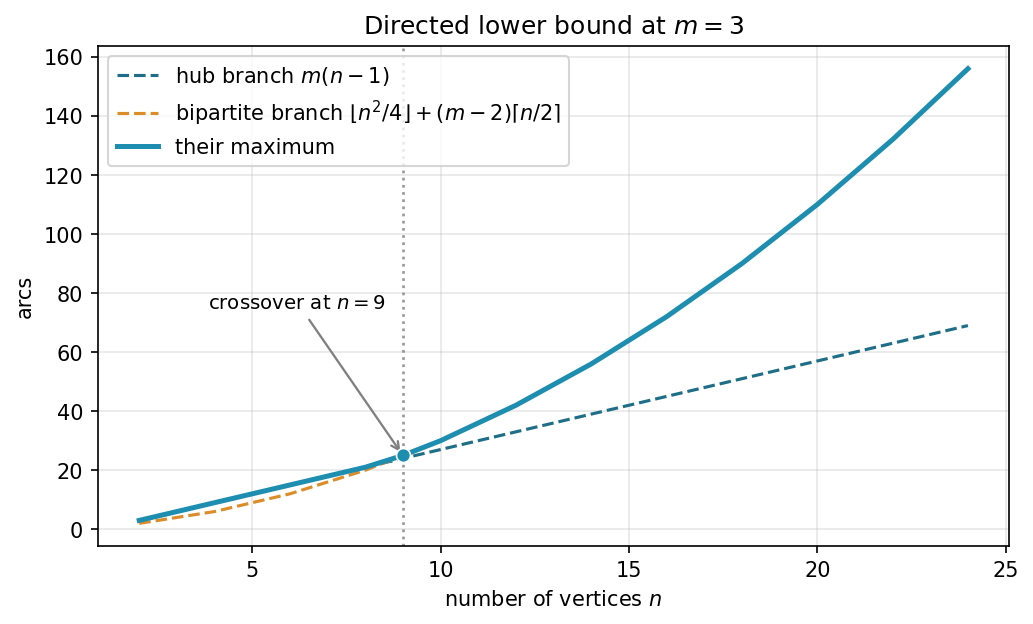
\includegraphics[width=0.78\textwidth]{figures/directed_crossover.png}
    \caption{The hub and augmented bipartite lower bounds at $m = 3$, and their maximum. The plot asserts no upper bound.}
    \label{fig:crossover}
\end{figure}

At $m=3$, exhaustive search proves the values $6,9,12,15$ for $n=3,4,5,6$.
The two separation conditions agree at every one of these orders (\Cref{rem:dir-vertex-m3}).
The search does not settle $n=7$.

The earlier decomposition conjecture has been removed as well.
It would force the quadratic upper bound as soon as that branch exceeds the
hub bound, which already happens at $m=5$, $n=12$.
The counterexample therefore refutes that structural assertion too.

The augmented bipartite count has the same leading term and the same order of error as the optimum.
\Cref{thm:dir-arc-linear-error} proves this without assuming the shape of an extremal graph.
The linear coefficient remains unknown among the results proved in this thesis.
Even identifying it would leave the exact bounded correction to establish.
More precisely, the construction gives a linear contribution $(m-2)n/2+O_m(1)$ above $n^2/4$, while the proved upper bound allows $4(m-1)n$. These inequalities do not show that a unique limiting linear coefficient exists.
Once $n$ is large in terms of $m$, the Tur\'an theorem of Huang and Lyu \cite{HuangLyu26} lowers the upper end to $m-1$ (\Cref{ch:basecases}).
The next section considers the separate question of extremal shape.

The directed vertex problem has the same leading term and error order by \Cref{thm:dir-vertex-linear-error}.
\Cref{app:proofs} treats it separately from the arc problem.
It remains open whether the two values are exactly equal for $m \ge 3$.

Allowing parallel arcs closes the arc-disjoint problem completely.
\Cref{thm:dir-multi-full} gives the exact value for every $n \ge 2$ and $m \ge 2$.

\section{Why direction makes the value quadratic}

In an undirected graph, every edge contributes to the degree of both endpoints.
Mader's theorem turns this symmetry into the linear cap $\floor{m(n-1)/2}$.
A digraph has no corresponding symmetry.

In \Cref{const:bipartite}, all arcs go from one part to the other and none return.
A directed route can therefore cross between the parts only once.
The construction has $\floor{n^2/4}$ arcs at $\lec^{\max}=1$.
No undirected graph of connectivity one can have quadratic size.
The linear cap does not survive the introduction of direction.
At $m=2$ and $n=8$, the one-directional construction has $16$ arcs while the hub has $14$.
The directed value must therefore follow the larger branch.

\Cref{const:augmented-bipartite} extends this idea to every $m$.
Each vertex of the larger part receives $m-2$ extra in-arcs from within that part.
\Cref{fig:augmented-wall} draws the construction.
The added arcs provide $m-2$ short detours for each relevant pair.
They raise $\lec^{\max}$ to $m-1$ and the arc count to $\floor{(n+m-2)^2/4}$.
At $m=3$ and $n=10$, the construction has thirty arcs while the hub has twenty-seven.

\begin{figure}[t]
\centering
\begin{tikzpicture}[>=Stealth, scale=1.0,
    wallarc/.style={gdirfaint},
    cyc/.style={-{Stealth[length=2.4mm]}, line width=1.3pt, vertexorange!85!black}]

  % The m = 3, n = 10 instance: |A| = 4, |B| = 6. B is drawn as the ring its
  % m-2 = 1 cyclic in-arc per vertex actually forms, rather than as a second
  % column, where six arcs along one side merge into a single visible stroke.
  \foreach \i/\y in {1/1.65, 2/0.55, 3/-0.55, 4/-1.65} {
    \node[smallvertex] (a\i) at (0,\y) {$a_{\i}$};
  }
  \foreach \j/\ang in {1/90, 2/30, 3/-30, 4/-90, 5/-150, 6/150} {
    \node[smallvertex] (b\j) at ($(5.6,0)+(\ang:1.85)$) {$b_{\j}$};
  }
  \begin{scope}[on background layer]
    \node[draw=KULblauw1!25, fill=KULblauw1!6, rounded corners=10pt,
          fit={(a1) (a4)}, inner sep=9pt] {};
    \node[draw=vertexorange!35, fill=vertexorange!5, circle,
          fit={(b1) (b2) (b3) (b4) (b5) (b6)}, inner sep=1pt] {};
  \end{scope}
  \node[font=\scriptsize, KULblauw1] at (0,2.55) {part $A$};
  \node[font=\scriptsize, vertexorange!75!black] at (5.6,2.55) {part $B$};

  % every arc from A to B: 4 x 6 = 24
  \foreach \i in {1,...,4}{\foreach \j in {1,...,6}{\draw[wallarc] (a\i) -- (b\j);}}

  % inside B, each b_j takes its m-2 = 1 cyclic predecessor: 6 more arcs
  \foreach \j/\k in {1/2, 2/3, 3/4, 4/5, 5/6, 6/1} {
    \draw[cyc] (b\j) -- (b\k);
  }

  \node[font=\scriptsize] at (0,-2.55) {$24$ arcs $A \to B$};
  \node[font=\scriptsize, align=center, vertexorange!75!black] at (5.6,-2.55)
    {$6$ cyclic in-arcs inside $B$};
\end{tikzpicture}
\caption{The augmented bipartite digraph of \Cref{const:augmented-bipartite} at $m = 3$, $n = 10$. Every cross-part arc runs from $A$ to $B$, and inside $B$ each vertex takes one arc from its cyclic predecessor, which is $m - 2$ arcs per vertex. A pair $a_i, b_j$ then has the direct arc and one detour, so $\lec^{\max} = 2$, and the count is $24 + 6 = 30$ against the hub branch's $27$.}
\label{fig:augmented-wall}
\end{figure}

The quadratic term is what the directed upper bound has to account for.
For eventual exactness, the argument must explain why no configuration has more
arcs than the augmented bipartite construction once $n$ is sufficiently large
in terms of $m$. The clique-core examples show why a restriction on $n$ is needed.
\Cref{prop:dir-arc-stability} and \Cref{thm:dir-arc-linear-error} support this structure in two ways.
In \emph{size}, the extremal value lies within $O_m(n)$ of the wall's count.
The remaining uncertainty includes the linear coefficient and the bounded correction.
In \emph{shape}, every feasible digraph becomes a subgraph of a one-directional bipartite graph after deleting $O(\sqrt{m}\,n^{3/2})$ arcs.
This weaker error comes from an argument that does not induct on a low-degree vertex.
The undirected problem has no analogous obstacle, because Mader's degree-counting argument closes it in a few lines.
The quadratic phenomenon is therefore the reason the directed and undirected problems differ in difficulty.

\section{Summary of the sixteen variants}

\Cref{fig:variant-tree-status} sorts all sixteen structural variants by how much
is known, and \Cref{tab:summary} states the strongest result for each. The entries
distinguish exact values, asymptotic bounds and constructions for cases whose
exact value remains open.
Each exact value is supported by a proof or by a completed exhaustive search.
Construction entries provide lower bounds, not claims of optimality.
Heuristic witnesses are never presented as upper bounds.
The markings follow the standard set in \Cref{ch:machine}.
For results with an AI badge, the author's verification caveat in the
Contribution Statement still applies. The summary does not upgrade their proof status.

\begin{figure}[t]
\centering
\resizebox{\textwidth}{!}{%
\begin{tikzpicture}
  \node[vtroot, fill=KULblauw3a!18]  (root) at (9.0,3.9) {Problem 915};
  \node[vtmodel, fill=KULblauw3a!12] (simple) at (1.8,2.6)  {simple};
  \node[vtmodel, fill=KULblauw3a!12] (multi)  at (6.6,2.6)  {multi};
  \node[vtmodel, fill=KULblauw3a!12] (hyper)  at (11.4,2.6) {hyper};
  \node[vtmodel, fill=KULblauw3a!12] (mhyper) at (16.2,2.6) {multi-hyper};
  \draw[vtedge] (root) -- (simple);
  \draw[vtedge] (root) -- (multi);
  \draw[vtedge] (root) -- (hyper);
  \draw[vtedge] (root) -- (mhyper);
  \node[vtdir, fill=KULblauw3a!8]  (d0) at (0.6,1.3)  {undirected};
  \node[vtdir, fill=KULblauw3a!8]  (d1) at (3.0,1.3)  {directed};
  \node[vtdir, fill=KULblauw3a!8]  (d2) at (5.4,1.3)  {undirected};
  \node[vtdir, fill=KULblauw3a!8]  (d3) at (7.8,1.3)  {directed};
  \node[vtdir, fill=KULblauw3a!8]  (d4) at (10.2,1.3) {undirected};
  \node[vtdir, fill=KULblauw3a!8]  (d5) at (12.6,1.3) {directed};
  \node[vtdir, fill=KULblauw3a!8]  (d6) at (15.0,1.3) {undirected};
  \node[vtdir, fill=KULblauw3a!8]  (d7) at (17.4,1.3) {directed};
  \draw[vtedge] (simple) -- (d0);
  \draw[vtedge] (simple) -- (d1);
  \draw[vtedge] (multi)  -- (d2);
  \draw[vtedge] (multi)  -- (d3);
  \draw[vtedge] (hyper)  -- (d4);
  \draw[vtedge] (hyper)  -- (d5);
  \draw[vtedge] (mhyper) -- (d6);
  \draw[vtedge] (mhyper) -- (d7);
  \node[vtleaf, fill=regimeProved!16]      (l0)  at (0,0)    {edge};
  \node[vtleaf, fill=regimePartial!20]     (l1)  at (1.2,0)  {vertex};
  \node[vtleaf, fill=regimeOpen!22]        (l2)  at (2.4,0)  {edge};
  \node[vtleaf, fill=regimeOpen!22]        (l3)  at (3.6,0)  {vertex};
  \node[vtleaf, fill=regimeProved!16]      (l4)  at (4.8,0)  {edge};
  \node[vtleaf, fill=regimePartial!20]     (l5)  at (6.0,0)  {vertex};
  \node[vtleaf, fill=regimeProved!16]      (l6)  at (7.2,0)  {edge};
  \node[vtleaf, fill=regimeOpen!22]        (l7)  at (8.4,0)  {vertex};
  \node[vtleaf, fill=regimePartial!20]     (l8)  at (9.6,0)  {edge};
  \node[vtleaf, fill=regimePartial!20]     (l9)  at (10.8,0) {vertex};
  \node[vtleaf, fill=regimeOpen!22]        (l10) at (12.0,0) {edge};
  \node[vtleaf, fill=regimeOpen!22]        (l11) at (13.2,0) {vertex};
  \node[vtleaf, fill=regimePartial!20]     (l12) at (14.4,0) {edge};
  \node[vtleaf, fill=regimePartial!20]     (l13) at (15.6,0) {vertex};
  \node[vtleaf, fill=regimeOpen!22]        (l14) at (16.8,0) {edge};
  \node[vtleaf, fill=regimeOpen!22]        (l15) at (18.0,0) {vertex};
  \draw[vtedge] (d0) -- (l0);  \draw[vtedge] (d0) -- (l1);
  \draw[vtedge] (d1) -- (l2);  \draw[vtedge] (d1) -- (l3);
  \draw[vtedge] (d2) -- (l4);  \draw[vtedge] (d2) -- (l5);
  \draw[vtedge] (d3) -- (l6);  \draw[vtedge] (d3) -- (l7);
  \draw[vtedge] (d4) -- (l8);  \draw[vtedge] (d4) -- (l9);
  \draw[vtedge] (d5) -- (l10); \draw[vtedge] (d5) -- (l11);
  \draw[vtedge] (d6) -- (l12); \draw[vtedge] (d6) -- (l13);
  \draw[vtedge] (d7) -- (l14); \draw[vtedge] (d7) -- (l15);
  % Legend, two columns of two. Column 1 is what is settled, column 2 is what is
  % not, so the partial entry sits beside the open one.
  \node[vtleaf, fill=regimeProved!16, minimum width=8mm]      (leg1) at (0,-1.5) {};
  \node[anchor=west, font=\scriptsize] at (0.9,-1.5) {closed form proved for every $n$ and $m$};
  \node[vtleaf, fill=regimeOpen!22, minimum width=8mm]        (leg3) at (9.4,-1.5) {};
  \node[anchor=west, font=\scriptsize] at (10.3,-1.5) {leading constant proved, exact value open};
  \node[vtleaf, fill=regimePartial!20, minimum width=8mm]     (leg4) at (9.4,-2.5) {};
  \node[anchor=west, font=\scriptsize] at (10.3,-2.5) {exact on stated parameter ranges, open outside them};
\end{tikzpicture}%
}
\caption{Status of the sixteen variants. Blue marks a closed form proved for every $n$ and $m$. Purple marks an exact value proved on stated parameter ranges and open outside them. Amber marks a proved leading term with the general exact value unknown. For simple directed arcs, \Cref{const:directed-comparison} records lower bounds without asserting optimality. The model and direction rows carry no status. \Cref{tab:summary} is authoritative for exceptions and conventions.}
\label{fig:variant-tree-status}
\end{figure}

\begin{table}[htbp]
\centering
\small
\renewcommand{\arraystretch}{1.3}
\setlength{\tabcolsep}{5pt}
\begin{tabularx}{\textwidth}{@{}>{\raggedright\arraybackslash}p{0.155\textwidth}>{\raggedright\arraybackslash}X>{\raggedright\arraybackslash}X@{}}
\toprule
Model & Edge or arc-disjoint & Vertex-disjoint \\
\midrule
\addlinespace[1pt]
\multicolumn{3}{@{}l}{\itshape Undirected} \\
\addlinespace[2pt]
simple graph
  & $\floor{m(n-1)/2}$, proved
  & the edge value for $m \le 4$, and at $m=5$ the edge value for $6 \le n \le 13$ then $\floor{8n/3}-4$ from $n=14$, while it is open for $m \ge 6$ \\
multigraph
  & $(m-1)(n-1)$, proved
  & $n-1$ at $m=2$ and $2(n-1)$ at $m=3$ (proved), while it is open for
    $m \ge 4$, where it is a knapsack over $2$-connected blocks and has order
    $\Theta(m^2n)$ in the joint regime stated below \\
$r$-hypergraph
  & $\le \floor{(m-1)(n-1)/(r-1)}$, with equality in the range below
  & $\floor{(n-1)/(r-1)}$ at $m=2$ and $\le \floor{2(n-1)/(r-1)}$ at $m=3$, while it is open for $m \ge 4$ \\
$r$-multi-hyper
  & the same bound, with equality when \mbox{$(r-1) \mid (n-1)$}
  & the same bounds, with repeated hyperedges settling cases missed by the simple model at $m=3$ \\
\addlinespace[4pt]
\midrule
\addlinespace[1pt]
\multicolumn{3}{@{}l}{\itshape Directed} \\
\addlinespace[2pt]
simple digraph
  & $M(n)$ at $m=2$ (proved), and $n^2/4 + \Theta_m(n)$ for $m \ge 3$, with dense constructions but no general exact formula
  & $M(n)$ at $m=2$ (proved), and $n^2/4 + \Theta_m(n)$ for $m \ge 3$ with equality to the arc value open \\
multigraph
  & $(m-1)M(n)$, proved
  & $M(n)$ at $m=2$ (proved), and $(m-1)n^2/4 + O_m(n)$ for $m \ge 3$ with the
    exact value open \\
$r$-hypergraph
  & $(1+o(1))(m-1)n^2/[4(r-1)]$ for fixed $r, m$, leading term proved
  & the same leading term for fixed $r, m$ \\
$r$-multi-hyper
  & the same leading term, the bound proved with repeats allowed
  & the same leading term for fixed $r, m$ \\
\bottomrule
\end{tabularx}
\caption{The sixteen variants and the strongest result known for each. The two multigraph vertex rows count multiplicity, since $q$ parallel copies are $q$ separated routes under the incidence convention of \Cref{sec:incidence-convention}. Ranges of validity, including the one at $m=5$, are stated below the table.}
\label{tab:summary}
\end{table}

Here $M(n)=\max(2(n-1),\floor{n^2/4})$. The hypergraph rows use $r\ge3$. At $r=2$, use the corresponding graph rows, in particular the different leading constant for simple digraphs when $m\ge3$. The multigraph incidence estimate uses $m\to\infty$ with $n/m\to\infty$. Simple-graph formulas assume
$n\ge m$. Below that range the complete object gives the trivial maximum.
The $m=5$ vertex row is quoted from $n\ge6$ because that is the range
\cite{SorensenThomassen74} states, not because it fails below it: extending the
small-range branch to $n=5$ reads $\floor{5\cdot4/2}=10$, which is what $K_5$
gives at $\kap^{\max}=4$.
The edge-hypergraph bound is attained when $(r-1)\mid(n-1)$ for
multihypergraphs, and for simple hypergraphs when $r\ge3$ and
$m-1\le\binom{n-2}{r-2}$. The $m=3$ vertex-hypergraph bound is attained by a simple hypergraph when
$2<r<n$, and by a multihypergraph whenever
$(r-1)\mid(n-1)$ (\Cref{prop:hyper-vertex-lower-multi}). Full statements and
exceptions are in 
\Cref{thm:mader,thm:leonard,thm:sorensen-thomassen,prop:hyper-edge,thm:simple-hyper-edge,thm:hyper-vertex-m2,thm:hyper-vertex-m3,thm:dir-multi-full,thm:dir-arc-linear-error,thm:dir-vertex-linear-error,thm:dir-hyper-constant}.

\subsection{Detailed finite values}

\Cref{tab:summary} and \Cref{fig:variant-tree-status} give the conclusion for every variant.
The computational audit records the underlying finite values at $m=3$ and $m=6$.
It also contains the four detailed grids (\Cref{sec:variant-grids}).
Keeping those repeated data in the appendix lets this chapter focus on the mathematical distinctions between the variants.

\subsection{Orientations of a directed hyperedge}
\label{sec:orientation-models}

\Cref{thm:dir-hyper-constant} pins the leading term in the directed hypergraph rows of \Cref{tab:summary}.
The table uses the \emph{forward} convention: one tail and $r-1$ heads.
Reversing every hyperedge gives the equivalent one-head \emph{backward} convention (\Cref{lem:dir-hyper-duality}).
\Cref{thm:dir-hyper-general-constant} gives the same leading term for the general model, which allows all nonempty tail--head splits.
It covers both separation conditions.
Orientation therefore creates no new asymptotic row in \Cref{tab:summary}.
The conventions may still differ at small orders.
Whether they agree exactly once $n>r$ remains open.

\section{Contributions and limitations of the program}

The program replaces separate implementations with one shared interface.
It represents graph models by a multiplicity matrix.
It represents undirected hypergraph models by collections of vertex sets and directed ones by tail and head sets.
An exact checker measures connectivity.
A certifier proves upper bounds for small cases.
Tabu search for graphs and random greedy search for hypergraphs find examples and hence lower bounds.
The seven validation runs in \Cref{sec:rediscovery} recover their known answers.

The three tools provide different levels of evidence.
The checker measures one supplied graph exactly.
A completed exhaustive search proves the best value at one finite order.
The certifier is also a finite check.
Without a replayable bound, it is not a reusable proof.
Heuristic search supplies lower bounds only.
A value is settled only when its lower and upper bounds agree.
Directed vertex values require separate checks because Whitney's inequality transfers witnesses but not upper bounds.
The repository contains the code and commands for rerunning the computational workflows.
This does not guarantee identical outcomes for time-limited searches. Some historical results also lack saved witnesses or measured runtimes, as recorded in the accompanying data.
The principal checks run from \code{program/erdos915\_unified.py}.
Several individual claims are backed by standalone scripts in \code{program/scripts/} instead.
Each is named where its result appears. Some implement separate checks, while experiment drivers reuse the shared solver.
\Cref{app:verification-ladder,app:software-tests} gives the environment, commands and audit evidence.
No theorem here depends only on an unchecked solver result.

The program also has clear limits.
The heuristic search cannot prove upper bounds.
The certifier proves an upper bound only at one fixed order.
Without a replayable certificate, that solver check does not become a reusable argument (\Cref{sec:certification-standard}).
For directed multigraphs, the finite encoding reaches only $n=6$.
At larger orders, the hand proof in \Cref{app:proofs} establishes the value.
The certifier did not finish at $n=7$.

Computation also leaves the structural gaps untouched.
Small-order agreement did not prevent the old directed arc formula from failing.
Even when one displayed construction eventually beats the others, its optimality among all feasible digraphs remains open here.
The directed vertex problem for $m\ge3$ does not follow from the arc case.
The undirected vertex problem for $m\ge6$ has been open for half a century.
The program can explore these problems, but it cannot settle them alone.

\section{Open problems}

\Cref{tab:open-problems} separates the proved results from the remaining frontiers.
Each row gives the strongest result established here.
It then states the next mathematical target.

\begin{table}[ht]
\centering
\scriptsize
\renewcommand{\arraystretch}{1.25}
\begin{tabularx}{\textwidth}{@{}>{\raggedright\arraybackslash}p{0.24\textwidth}>{\raggedright\arraybackslash}p{0.31\textwidth}>{\raggedright\arraybackslash}X@{}}
\toprule
Problem & Known here & Remaining target \\
\midrule
Directed simple arc, $m\ge3$ & $\ell_m^{\mathrm{dir}}(n)=n^2/4+\Theta_m(n)$ (\Cref{thm:dir-arc-linear-error}) & Determine when, if ever, the constructions of \Cref{const:directed-comparison} attain the optimum. \\
Directed simple vertex, $m\ge3$ & $k_m^{\mathrm{dir}}(n)=n^2/4+\Theta_m(n)$ (\Cref{thm:dir-vertex-linear-error}) & Decide whether its exact value equals the arc value, given that an arc upper bound does not transfer. \\
Directed multigraph classification & Exact value for all $n,m$ and quadratic-branch uniqueness for $n\ge\max(8,2m)$ & Classify the range $n<2m$ and the remaining linear-branch extremisers. \\
Directed multigraph incidence, $m\ge3$ & $K_m^{\mathrm{dir}}(n)=(m-1)n^2/4+O_m(n)$ (\Cref{cor:dir-multi-incidence}) & Sharpen the next-order term and decide whether the arc extremiser is optimal here too. \\
Undirected simple vertex, $m\ge6$ & Block formulation and $m/2<c_m\le2(m-1)$, where $c_m = \lim_n k_m(n)/(n-1)$ (\Cref{thm:simple-vertex-blocks}) & Determine $c_m$ by finding sharper bounds on feasible blocks. \\
Undirected multigraph incidence, $m\ge4$ & Reduction to a knapsack over $2$-connected blocks. The value is $\Theta(m^2n)$ as $m\to\infty$ with $n/m\to\infty$ (\Cref{thm:multi-vertex-blocks,thm:multi-vertex-bipartite,prop:multi-vertex-upper}) & Determine the best $2$-connected block of each size and sharpen the asymptotic bounds. \\
Hypergraph vertex, $m\ge4$ & Exact at $m=2$ and, in the stated range, $m=3$ (\Cref{thm:hyper-vertex-m2,thm:hyper-vertex-m3}) & Determine which edge-separation bounds remain valid for vertex separation when $r\ge3$. \\
Directed hypergraphs & For fixed $r\ge3$ and $m\ge2$, leading term $(m-1)n^2/(4(r-1))$ for all orientations and both separations & Determine finite exact values and whether forward and general agree once $n>r$. \\
\bottomrule
\end{tabularx}
\caption{The remaining problems, separated from the results already proved in this thesis.}
\label{tab:open-problems}
\end{table}

Four directions carry most of the remaining mathematical weight.
The first is the simple directed arc problem.
\Cref{const:directed-comparison} supplies three dense families, but no matching general upper bound.
The clique-core counterexample leaves the smaller orders as a separate question.

The second direction is the classical undirected vertex problem for $m\ge6$.
It remains open despite the results of S{\o}rensen and Thomassen.
The third is the hypergraph vertex problem beyond $m=3$.
There the incidence-rank argument has no known higher-connectivity replacement.
The fourth is the multigraph incidence problem beyond $m=3$, which the convention
of \Cref{sec:incidence-convention} poses as a question of its own.
Its value is a knapsack over $2$-connected blocks, and what is missing is the
best block of each size. As $m\to\infty$ with $n/m\to\infty$, the ratio
$K_m(n)/(m^2n)$ is at least $3-2\sqrt{2}-o(1)$ and less than $2$.
These bounds do not establish that the ratio converges.

The other rows of \Cref{tab:open-problems} remain natural questions.
They ask for finer classifications or finite exact values.
They complete the map, but they are secondary to the four frontiers above.


% ============================================================================
% APPENDICES
% ============================================================================

\appendix
\crefalias{chapter}{appendix}

\chapter{Proofs, Proposed Proofs and Computational Audit}\label{app:proofs}
This appendix carries every proof in the thesis. The body states the results and says in a few sentences what makes each one work, and the argument itself is here, together with the supporting lemmas and propositions that no chapter states in its own right, and with figures beside the arguments that need them.

\paragraph{How to read this appendix.} It runs in four parts, and they are not of equal weight. \textsc{Part I} is classical machinery, \Cref{thm:menger,thm:gomory-hu} and Mader's theorem, and may be skipped by a reader who trusts the cited results. \textsc{Parts II} and \textsc{III} carry the original arguments, and a reader with time for three of them should read \Cref{thm:dir-multi-full} (the directed multigraph value, closed for every $n$ and $m$ by deleting a reachability skeleton rather than a vertex), \Cref{lem:incidence-rank} with \Cref{thm:hyper-vertex-m3} (the incidence rank bound proved through Tutte's triconnected decomposition, which settles the hypergraph vertex problem at $m = 3$), and \Cref{lem:two-step-budget} with the three theorems it drives, \Cref{thm:dir-arc-linear-error,thm:dir-vertex-linear-error,thm:dir-hyper-constant}, which pin six of the sixteen variants asymptotically with no hypothesis on the shape of the extremiser. \textsc{Part IV} holds one self-contained extension, the search's connectivity bookkeeping, and the computational audit. Every construction the body refers to by name is defined here, the directed ones in \Cref{sec:dir-constructions}. A heading carrying the badge \aimedal{} means that the proof under it was written by an AI model and is not verified line by line by the author, as the Contribution Statement sets out. In this appendix the badge is on every result except the cited classical ones and the Gomory--Hu double count of \Cref{sec:mader-gomory-hu}, which proves \Cref{thm:mader,thm:multigraph-edge} out of \Cref{lem:dist-1-count,lem:sum-dist,lem:double-count}.

% ---------------------------------------------------------------------------
% These appendix figures use the SHARED thesis TikZ styles (../shared/tikz-
% styles.tex), so they match the blue KU Leuven look of the body figures.  The
% appendix-prefixed names below are thin aliases onto those shared styles, kept
% only so the dense figure bodies need no editing: apxlab/apx are thesis blue
% vertices (labelled / small), apz a hyperedge square (hnode), apgedge the
% standard edge, aparc a directed arc, apredarc/apdashed forbidden objects.
% ---------------------------------------------------------------------------
\tikzset{
  apx/.style={gvertex, minimum size=4mm},
  apxlab/.style={gvertex},
  apz/.style={hnode},
  apgedge/.style={gline},
  aptedge/.style={line width=1.3pt, KULblauw3b, line cap=round},
  aparc/.style={gdir},
  apfaint/.style={gdirfaint},
  apredarc/.style={gcut},
  apdashed/.style={gcutedge},
  aplab/.style={edgelabel},
  aptw/.style={treeweight},
  % apname: a free-floating text label with NO white fill box, for vertex names
  % and annotations placed in open space. (Using aplab there draws an ugly white
  % rectangle, and passing a bare colour to aplab overrides its fill and turns
  % the whole label into a solid colour block, so coloured annotations use
  % apname with text=<colour>.)
  apname/.style={font=\scriptsize, inner sep=1.5pt},
}

% ---------------------------------------------------------------------------
% Part dividers. The appendix is one chapter, so its ten sections would
% otherwise present as a flat list longer than any body chapter. \apppart draws
% a labelled rule before each group and writes the group into the table of
% contents, so a reader can find the directed work or the hypergraph work
% without scanning every section heading. It introduces no numbering and no new
% label, so every \Cref{app:proofs} in the body still resolves to this chapter.
% ---------------------------------------------------------------------------
\newcommand{\apppart}[2]{%
  \par\addvspace{1.2\baselineskip}%
  \phantomsection% own anchor, so the bookmark does not collide with the chapter's
  \addcontentsline{toc}{section}{\protect\numberline{}\textsc{#1}}%
  \noindent{\color{KULblauw1}\rule{\linewidth}{1.1pt}}\par\nobreak
  \vspace{2pt}\noindent{\normalfont\bfseries\color{KULblauw1}#1}\par\nobreak
  \vspace{1pt}\noindent{\normalfont\small\itshape\color{black!70}#2}\par\nobreak
  \vspace{2pt}\noindent{\color{KULblauw1}\rule{\linewidth}{0.4pt}}\par\nobreak
  \addvspace{0.4\baselineskip}}

\apppart{Part I. Classical machinery}{The two theorems every later argument runs on, and Mader's theorem proved in full through the Gomory--Hu tree. Cited results, reproved here so the thesis stands on its own.}

\section{Menger, Gomory--Hu, and the degree bound}

We use two classical results in their capacitated form. Unit capacities represent simple graphs, integer capacities represent multiplicities, and cut capacity is the total capacity crossing the cut.

\begin{theorem}[Menger and max-flow/min-cut \cite{Menger27,FordFulkerson56}]\label{thm:menger}
In any capacitated digraph, and for distinct vertices $u, v$, the maximum flow from $u$ to $v$ equals the minimum capacity of a cut separating $u$ from $v$. This is the max-flow/min-cut theorem. With integer capacities, integral flow decomposition recovers Menger's path--separator theorem. At unit capacities it gives the combinatorial statement we cite throughout: the maximum number of pairwise edge-disjoint $u$--$v$ paths equals the minimum number of edges whose removal separates them,
\[
    \lec_G(u, v) = \min\{\, |C| : C \subseteq E(G),\ G - C \text{ has no } u\text{--}v \text{ path} \,\}.
\]
Undirected graphs become symmetric networks, multigraph multiplicities become capacities, hypergraphs use the gate network of \Cref{fig:hyper-gadget}, and vertex-disjoint routes use the vertex splitting of \Cref{fig:vertex-split}. Thus one maximum-flow theorem supports every checker variant.
\end{theorem}

\begin{theorem}[Gomory--Hu \cite{GomoryHu61}]\label{thm:gomory-hu}
Every \emph{undirected} capacitated graph $G$ has a weighted tree $T$ on the same vertex set, its \emph{Gomory--Hu tree}, such that for all $u, v$ the value $\lec_G(u, v)$ equals the minimum edge weight on the $u$--$v$ path in $T$, and each tree edge $e$ corresponds to a minimum cut of $G$ whose capacity is the weight of $e$. All $\binom{n}{2}$ pairwise values are thereby stored in the $n-1$ weights of a single tree.
\end{theorem}

The theorem applies to undirected simple graphs, multigraphs, and hyperedge cuts (\Cref{thm:hyper-gomory-hu}), but not to asymmetric directed cuts or vertex connectivity. Its standard submodular-cut construction is proved in \cite{GomoryHu61}. Here we use only the displayed path-minimum identity.

We also use the immediate endpoint bound.

\begin{lemma}[Degree bound,\aimedal]\label{lem:degree-bound}
For every pair of vertices of a graph $G$, $\lec_G(u, v) \le \min(\deg u, \deg v)$. In a digraph $D$, $\lec_D(u, v) \le \min(d^+(u), d^-(v))$.
\end{lemma}

\begin{proof}
Every edge-disjoint $u$--$v$ path uses a distinct edge at $u$, so there are at most $\deg u$ of them, and likewise at most $\deg v$. In the directed case each arc-disjoint path leaves $u$ by a distinct out-arc and enters $v$ by a distinct in-arc.
\end{proof}

\Cref{ch:machine} leans on two monotonicity facts to keep the search's connectivity checks cheap. Both follow directly from max-flow / min-cut.

\begin{proposition}[Monotonicity of the binding connectivity,\aimedal]\label{prop:monotone}
Let $G$ be any graph, digraph, hypergraph, or directed hypergraph model used in this thesis, simple or with multiplicities, and let $G'$ be obtained from $G$ by changing one edge, arc, or hyperedge by a single copy. Then
% \Cref{ch:machine} cites these as "part (1)" and "part (2)", so this list
% carries explicit numbers in place of the decorative global list icon.
\begin{enumerate}[label=(\arabic*)]
    \item \textup{(monotonicity)} removing the unit cannot raise $\lambda^{\max}$, and adding it cannot lower $\lambda^{\max}$, and
    \item \textup{(unit step)} adding the unit raises $\lambda^{\max}$ by at most one.
\end{enumerate}
Both statements hold verbatim for the vertex measure $\kappa^{\max}$.
\end{proposition}

\begin{proof}
Write $G^+$ for $G$ with one edge, arc, or hyperedge copy added, and fix a pair $(s,t)$, ordered in a directed model. Removing a copy only removes routes, so neither local connectivity can increase under removal. This proves the monotonicity part after taking the maximum over all pairs.

For the unit step in edge connectivity, take a largest edge-, arc-, or hyperedge-disjoint family of $s$--$t$ routes in $G^+$. At most one member of the family uses the new copy. Discard that member if it exists. Every remaining route lies in $G$, so
\[
    \lambda_G(s,t) \le \lambda_{G^+}(s,t) \le \lambda_G(s,t)+1.
\]

The vertex measure has the same unit step, but it is safer to see it directly than through a split-network cut. In a graph or digraph, two internally vertex-disjoint routes cannot both use the new adjacency. If it is internal to both routes, they share its endpoints internally. If it meets $s$ or $t$, they share its other endpoint internally, except for the unique one-step $s$--$t$ route. In the hypergraph convention of \Cref{sec:hyper-vertex-proof}, the routes are also hyperedge-copy-disjoint, so again at most one uses the new copy. Deleting that route leaves a family in $G$ and gives
\[
    \kappa_G(s,t) \le \kappa_{G^+}(s,t) \le \kappa_G(s,t)+1.
\]
Taking the maximum over all pairs proves the two asserted unit-step bounds. If the new copy is parallel to an existing adjacency under the reduced convention of \Cref{sec:parallel-convention}, it changes $\kappa^{\max}$ by zero, which is already covered by the inequality.
\end{proof}

\section{Mader's theorem in full}\label{sec:mader-gomory-hu}

Let $T$ be a Gomory--Hu tree of $G$ and let $\dist_T(e)$ count the tree edges on the path between the endpoints of $e\in E(G)$, as \Cref{fig:gomory-hu-dist} illustrates. The upper bound is the following double count. Simplicity enters only because at most $n-1$ graph edges can join adjacent vertices of $T$.

\begin{figure}[htbp]
\centering
\begin{tikzpicture}[scale=0.86, transform shape]
% --- left: graph G ---
\begin{scope}
  \node[apxlab] (e) at (-0.7,0.4) {e};
  \node[apxlab] (a) at (0.6,1.5) {a};
  \node[apxlab] (b) at (2.1,1.5) {b};
  \node[apxlab] (c) at (2.8,0.1) {c};
  \node[apxlab] (d) at (1.3,-0.9) {d};
  \draw[apgedge] (e)--(a);
  \draw[apgedge] (a)--(b);
  \draw[apgedge] (b)--(c);
  \draw[apgedge] (c)--(d);
  \draw[apgedge] (b)--(d);          % dist 2
  \draw[apgedge] (a)--(c);          % dist 2
  \draw[apgedge,vertexred] (e) to[bend right=22] (c);  % dist 3, highlighted
  \node[font=\small] at (1.0,-1.7) {graph $G$};
\end{scope}
% --- right: Gomory--Hu tree T (star centred at a and c) ---
\begin{scope}[xshift=6.4cm]
  \node[apxlab] (te) at (-0.7,0.4) {e};
  \node[apxlab] (ta) at (0.6,1.5) {a};
  \node[apxlab] (tb) at (2.1,1.5) {b};
  \node[apxlab] (tc) at (2.8,0.1) {c};
  \node[apxlab] (td) at (1.3,-0.9) {d};
  \draw[aptedge] (te)--(ta) node[aptw,midway] {2};
  \draw[aptedge] (ta)--(tc) node[aptw,pos=0.4] {3};
  \draw[aptedge] (tc)--(tb) node[aptw,midway] {3};
  \draw[aptedge] (tc)--(td) node[aptw,midway] {2};
  \node[font=\small] at (1.0,-1.7) {Gomory--Hu tree $T$};
\end{scope}
% bracket arrow
\draw[-{Stealth[length=6pt]}, line width=1.3pt, KULblauw3b]
   (3.4,0.4) -- (4.7,0.4);
\end{tikzpicture}
\caption[Graph and Gomory--Hu tree]{A graph $G$ and a Gomory--Hu tree $T$ on the same vertices. Each graph edge crosses $\dist_T(e)$ tree cuts, and at most $n-1$ edges of a simple graph have tree distance one.}
\label{fig:gomory-hu-dist}
\end{figure}

\begin{lemma}[Distance-one edges]\label{lem:dist-1-count}
At most $n-1$ edges of a simple graph $G$ satisfy $\dist_T(e) = 1$.
\end{lemma}

\begin{proof}
An edge $e \in E(G)$ has $\dist_T(e) = 1$ if and only if its endpoints are adjacent in $T$. The tree $T$ has exactly $n-1$ edges, and since $G$ is simple each pair of adjacent tree vertices supports at most one edge of $G$.
\end{proof}

\begin{lemma}[Sum of tree distances]\label{lem:sum-dist}
$\displaystyle\sum_{e \in E(G)} \dist_T(e) \;\ge\; 2|E(G)| - (n-1)$.
\end{lemma}

\begin{proof}
Partition $E(G)$ into $E_1 = \{e : \dist_T(e) = 1\}$ and $E_{\ge 2} = \{e : \dist_T(e) \ge 2\}$. Then
\[
\sum_{e \in E(G)} \dist_T(e) \;\ge\; |E_1| + 2\,|E_{\ge 2}| \;=\; 2|E(G)| - |E_1| \;\ge\; 2|E(G)| - (n-1),
\]
using \Cref{lem:dist-1-count} in the last step.
\end{proof}

\begin{lemma}[Double-counting identity]\label{lem:double-count}
Let $G$ carry \emph{unit capacities}, so that each weight $c(t)$ of a Gomory--Hu tree $T$ is the plain \emph{number} of edges of $G$ crossing the cut that $t$ induces. Then
\[
    \sum_{t \in E(T)} c(t) \;=\; \sum_{e \in E(G)} \dist_T(e).
\]
This is the form used for Mader's theorem, where $G$ is a simple graph and so unit-capacitated by default.
\end{lemma}

\begin{proof}
By \Cref{thm:gomory-hu} each tree edge $t$ induces a cut of $G$ of capacity $c(t)$, so $c(t) = \sum_{e \in E(G)} \mathbf{1}_{e \text{ crosses } t}$. Exchanging the order of summation,
\[
\sum_{t \in E(T)} c(t) = \sum_{e \in E(G)} \sum_{t \in E(T)} \mathbf{1}_{e \text{ crosses } t} = \sum_{e \in E(G)} \dist_T(e),
\]
where the last equality holds because an edge $\{u,v\}$ crosses exactly those tree cuts induced by the tree edges on the unique $u$--$v$ path in $T$.
\end{proof}

\begin{proof}[Proof of \Cref{thm:mader}, upper bound]
Let $G$ be a simple graph on $n$ vertices with $\lec^{\max}_G \le m-1$ and let $T$ be a Gomory--Hu tree of $G$. Each tree edge $t = \{x, y\}$ has weight $c(t) = \lec_G(x, y) \le m-1$, so summing over the $n-1$ tree edges, $\sum_{t} c(t) \le (m-1)(n-1)$. Combining with \Cref{lem:sum-dist,lem:double-count},
\[
2|E(G)| - (n-1) \;\le\; \sum_{e \in E(G)} \dist_T(e) \;=\; \sum_{t \in E(T)} c(t) \;\le\; (m-1)(n-1).
\]
Rearranging gives $2|E(G)| \le m(n-1)$, and since $|E(G)|$ is an integer, $|E(G)| \le \floorfrac{m(n-1)}{2}$.
\end{proof}

The factor two comes from charging all but at most $n-1$ edges to at least two tree cuts. Parallel edges destroy that refinement, leaving the multigraph bound $(m-1)(n-1)$ of \Cref{thm:multigraph-edge}.

\begin{proof}[Proof of \Cref{thm:multigraph-edge}]
For the lower bound, take a spanning tree of $K_n$, that is, a connected cycle-free subgraph that touches all $n$ vertices and so has exactly $n-1$ edges, and give every tree edge multiplicity $m - 1$, meaning $m-1$ parallel copies. The result has $(m-1)(n-1)$ edges. Any two vertices are joined by a unique path in the tree, of some length $k \ge 1$. To separate them one must cut some edge of that path, and the cheapest choice is the lightest tree edge on it, which still carries $m-1$ copies, so $\lec(u, v) = m - 1$ for every pair and $\lec^{\max} = m - 1$. The graph sits right at the cap.

For the upper bound, suppose $\lec_G^{\max} \le m - 1$ and build a Gomory--Hu tree $T$ of $G$ (\Cref{thm:gomory-hu}), the same $(n-1)$-edge summary of all connectivities used for Mader's theorem. Each tree edge $e$ stands for a minimum cut of $G$, of capacity $c(e) = \lec_G(u,v) \le m-1$ for the pair $(u,v)$ it represents. Now charge each edge of $G$ to a tree edge: an edge $\{x,y\}$ crosses the cut of the lightest tree edge on the tree path from $x$ to $y$, so it is counted inside that tree edge's capacity. Summing the $n-1$ capacities therefore counts every edge of $G$ at least once, which already gives $|E(G)| \le \sum_{e \in T} c(e) \le (m-1)(n-1)$. Unlike Mader's simple-graph count there is no second charge to halve, because parallel edges are now allowed and nothing forces an edge to be counted twice. The tree-of-multiplicity-$(m-1)$ construction above meets this bound exactly, which is why the answer is the clean product $(m-1)(n-1)$ and not a floor.
\end{proof}

\begin{construction}[Hub-and-spokes graph]\label{const:hub-spokes}
For $n \ge m \ge 2$, let $H_{m,n}$ have vertex set $\{h, v_1, \ldots, v_{n-1}\}$ with
(i) all $n-1$ \emph{hub edges} $\{h, v_i\}$, and
(ii) a \emph{spoke graph} on $\{v_1, \ldots, v_{n-1}\}$ with $\floorfrac{(m-2)(n-1)}{2}$ edges in which every $v_i$ has spoke degree at most $m-2$. Such a spoke graph exists by \Cref{lem:near-regular}.
This is the general extremal construction. If $(m-1)\mid(n-1)$, take the
spoke graph to be disjoint copies of $K_{m-1}$, and adjoining $h$ turns them into
copies of $K_m$ with one shared vertex, the shared-clique construction.
\label{const:shared-clique}
\end{construction}

\begin{lemma}[Near-regular graphs exist,\aimedal]\label{lem:near-regular}
For $N \ge 1$ and $0 \le r \le N-1$ there is a graph on $N$ vertices with $\floorfrac{rN}{2}$ edges and maximum degree at most $r$.
\end{lemma}

\begin{proof}
If $rN$ is even we build an $r$-regular circulant graph on vertex set $\{0, \dots, N-1\}$: for even $r$ connect each $i$ to $i \pm j \pmod N$ for $j = 1, \dots, r/2$, and for odd $r$ (then $N$ is even) use $j = 1, \dots, (r-1)/2$ together with the diameter distance $N/2$, which contributes degree one. Both are $r$-regular with $rN/2$ edges. If $rN$ is odd, then $r$ and $N$ are both odd: take the $(r-1)$-regular circulant with distances $1, \dots, (r-1)/2$ and add the near-perfect matching that pairs vertex $i$ with $i + (N+1)/2 \pmod N$ for $i = 0, \dots, (N-3)/2$, which covers all vertices but one. The total is $\frac{(r-1)N}{2} + \frac{N-1}{2} = \frac{rN-1}{2} = \floorfrac{rN}{2}$ edges, with one vertex of degree $r-1$ and all others of degree $r$.
\end{proof}

\begin{theorem}[Extremal graphs exist,\aimedal]\label{thm:extremal-existence}
For all $n \ge m \ge 2$ the graph $H_{m,n}$ has $\floorfrac{m(n-1)}{2}$ edges and $\lec^{\max} \le m-1$.
\end{theorem}

\begin{proof}
The edge count is $(n-1) + \floorfrac{(m-2)(n-1)}{2} = \floorfrac{m(n-1)}{2}$, since $(m-2)(n-1)$ and $m(n-1)$ have the same parity. For the connectivity, any two distinct vertices include at least one spoke vertex $v_i$, whose total degree is at most $1 + (m-2) = m-1$. \Cref{lem:degree-bound} then gives $\lec(u,v) \le m-1$.
\end{proof}

The upper bound above proves \Cref{thm:mader}, and it uses no relation between $n$ and $m$: the Gomory--Hu tree has $n-1$ edges whatever $m$ is. \Cref{thm:extremal-existence} adds that the bound is attained once $n \ge m$, which is where that hypothesis is needed and where it belongs. For $n<m$, the complete graph is itself feasible and the bound is slack except at $(n,m)=(2,3)$, where the floor creates the isolated equality noted in the main text. Equality then holds systematically from $n=m$ onward. The proof also reveals which graphs are extremal: equality forces both inequalities in the chain to be tight.

\begin{theorem}[Characterisation of equality,\aimedal]\label{thm:extremal-char}
Let $G$ be simple with $\lec^{\max}_G \le m-1$ and $|E(G)| = \floorfrac{m(n-1)}{2}$, and let $T$ be a Gomory--Hu tree of $G$. If $m(n-1)$ is even, then every tree edge has weight exactly $m-1$, every tree edge is also an edge of $G$, and every edge of $G$ joins vertices at tree distance at most $2$. If $m(n-1)$ is odd, there is exactly one unit of slack, located in exactly one of three places: one tree edge has weight $m-2$, or one tree edge is not an edge of $G$, or one edge of $G$ joins vertices at tree distance $3$. Everything else is tight.
\end{theorem}

\begin{proof}
Write the chain of the upper-bound proof as three non-negative integer slacks, one for each inequality it uses:
\[
    S_1 = (m-1)(n-1) - \sum_t c(t),
    \qquad
    S_2 = \sum_{e :\, \dist_T(e) \ge 2} \bigl(\dist_T(e) - 2\bigr),
    \qquad
    S_3 = (n-1) - |E_1| .
\]
In words, $S_1$ counts tree weights below $m-1$, $S_2$ counts edges beyond tree distance two, and $S_3$ counts tree edges that support no edge of $G$. Retracing the proof gives two expressions for the same quantity,
\[
    \sum_e \dist_T(e) \;=\; 2|E| - |E_1| + S_2
    \qquad\text{and}\qquad
    \sum_e \dist_T(e) \;=\; \sum_t c(t) \;=\; (m-1)(n-1) - S_1 .
\]
Substituting $|E_1| = (n-1) - S_3$ into the first and equating it with the second,
\[
\begin{aligned}
    2|E| - (n-1) + S_2 + S_3 &\;=\; (m-1)(n-1) - S_1, \\[2pt]
    \text{so}\qquad 2|E| &\;=\; m(n-1) - (S_1 + S_2 + S_3).
\end{aligned}
\]
The whole characterisation reads off that last identity. If $m(n-1)$ is even, equality $|E| = m(n-1)/2$ forces $S_1 = S_2 = S_3 = 0$. If $m(n-1)$ is odd the floor absorbs exactly one unit, so $S_1 + S_2 + S_3 = 1$ and exactly one of the three slacks equals one.
\end{proof}

For $m = 2$ the characterisation says the extremal graphs are exactly the spanning trees: every tree edge must carry weight one and lie in $G$, so $G$ contains its own Gomory--Hu tree and has only $n-1$ edges to spend. For $m = 4$ and $n \equiv 1 \pmod{3}$ it is consistent with the trees of $K_4$ blocks glued at shared cut vertices, the case of \Cref{const:shared-clique} that the search of \Cref{ch:discover} rediscovers.

\begin{remark}[The counting convention, and the audit it forces]\label{rem:threshold-convention}\label{rem:threshold-audit}
This thesis defines $\ell_m(n)$ and $k_m(n)$ as the \emph{largest} number of edges a graph can carry while \emph{no} pair is joined by $m$ independent routes. 
S{\o}rensen and Thomassen, and the Erd\H{o}s Problems database \cite{ErdosProblems} after them, state the same results the other way round, as the \emph{smallest} number of edges that \emph{forces} such a pair. 
Those two quantities are adjacent integers by construction: if $k$ is the largest feasible edge count then no graph on $n$ vertices with $k+1$ edges is feasible, so $k+1$ is exactly the forcing threshold.

What follows is the bookkeeping that convention forces on every constant quoted from the literature.

The shift is visible in every entry the database and this thesis both state. It gives $k_2(n) = n$ where a tree has $n-1$ edges, $k_3(2n) = 3n-1$ against $\floor{3(2n-1)/2} = 3n-2$ here, $k_4(n) = 2n-1$ against $2n-2$, $\ell_5(2n) = 5n-2$ against $5n-3$, $\ell_6(n) = 3n-2$ \cite{Leonard73} against $3n-3$, and it writes the Bollob\'{a}s-Erd\H{o}s conjecture as $1 + \binom{m}{2}n$ \emph{on $1 + (m-1)n$ vertices} against $\binom{m}{2}n$ here. Every one is exactly one apart, and the values in this thesis are the ones an exhaustive search returns: $k_3(4) = 4$, $k_3(5) = 6$ and $k_4(5) = 8$ were each confirmed by walking every graph of that size.

The conjecture is the one entry that must keep its vertex count attached, and an earlier draft of this thesis lost it. On $N = 1 + (m-1)n$ vertices the conjectured value is $\binom{m}{2}\frac{N-1}{m-1} = \frac{m(N-1)}{2}$, which is the rate $c_m = m/2$ of \Cref{thm:simple-vertex-blocks}. Read instead as a count on $n$ vertices, $\binom{m}{2}n$ overstates it by a factor of $m-1$, giving $3n$ at $m = 3$ where the true value is about $3n/2$.

A second trap is worth naming, because an earlier draft fell into that one too. The comparison $k_5 > \ell_5$ is invariant under the shift, since \emph{both} functions move by one, so no internal check can detect a half-converted statement. What does detect it is evaluating the two sides in different conventions, which manufactures a spurious divergence one size early. Reading $\floor{8 \cdot 13/3} - 3 = 31$ against this thesis's $\ell_5(13) = 30$ appears to separate the two problems at $n = 13$, but the $31$ is a forcing count and the $30$ is an avoiding count. Done consistently, $k_5(13) = 30 = \ell_5(13)$ and the separation begins at $n = 14$, which is also what \cite{SorensenThomassen74} proves directly by showing $f_5(n) = \floor{5(n-1)/2} + 1$ throughout $6 \le n \le 13$.

The range likewise comes from the paper rather than from the database, which records only the clean tail $n \ge 13$. Theorem 4 there states $f_5(n) = \floor{8n/3} - 3$ for every $n \ge 6$ apart from $n = 7$ and $n = 12$, and supplies $f_5(7) = 16$ and $f_5(12) = 28$ separately. Its closing line then covers the whole small range at once, $f_5(n) = \floor{5(n-1)/2} + 1$ for $6 \le n \le 13$. That is why \Cref{thm:sorensen-thomassen} is stated in two ranges and needs no exceptions: the two sizes the paper sets aside are the only points of $6 \le n \le 13$ at which the large-$n$ formula misses the small-$n$ one, low by one at $n = 7$ and high by one at $n = 12$.
\end{remark}

\subsection{The vertex problem is a block problem}\label{sec:simple-vertex-blocks}

The \emph{vertex} problem $k_m(n)$ has been open since 1974, and this short section records its block structure. It changes the object being searched: from graphs on $n$ vertices, with $n$ growing, to $2$-connected graphs alone.

\begin{theorem}[The vertex problem is a knapsack over blocks,\aimedal]\label{thm:simple-vertex-blocks}
For $b \ge 2$ let
\[
    h_m(b) \;:=\; \max\bigl\{\, |E(B)| \;:\; B \text{ $2$-connected or a single edge},\ |V(B)| = b,\ \kap^{\max}_B \le m-1 \,\bigr\} ,
\]
with $h_m(b) := -\infty$ when no such $B$ exists, as happens for every $b \ge 3$ at $m = 2$, where a cycle already carries two internally disjoint routes.
Then for all $m \ge 2$ and $n \ge 2$,
\[
    k_m(n) \;=\; \max\Bigl\{\, \sum_i h_m(b_i) \;:\; b_i \ge 2,\ \sum_i (b_i - 1) \le n-1 \,\Bigr\} .
\]
Consequently $k_m(n) \ge k_m(n_1) + k_m(n_2)$ whenever $n = n_1 + n_2 - 1$, and
\[
    c_m \;:=\; \lim_{n \to \infty} \frac{k_m(n)}{n-1} \;=\; \sup_{b \ge 2} \frac{h_m(b)}{b-1}
\]
exists, the limit being approached from below. The supremum is finite: \Cref{rem:vertex-degeneracy} gives $k_m(n) < 2(m-1)n$, so $c_m \le 2(m-1)$.
\end{theorem}

\begin{proof}
Let $G$ be feasible. Adjacent vertices $u,v$ lie in a common block $B$, and no $u$-$v$ path leaves $B$: leaving means crossing a cut vertex, and returning means crossing that same cut vertex a second time, which no path does. So $\kap_G(u,v) = \kap_B(u,v)$, every block inherits feasibility, and since every edge lies in exactly one block, $|E(G)| = \sum_B |E(B)| \le \sum_B h_m(|V(B)|)$. Within one component the block sizes satisfy $\sum_B (|V(B)|-1) = (\text{order of the component}) - 1$, and summing over components loses one further vertex apiece, so $\sum_B (|V(B)|-1) \le n-1$. That is $\le$.

For $\ge$, take blocks $B_1, \dots, B_t$ with $\sum (b_i - 1) \le n-1$, pick one vertex, and attach all the $B_i$ to it, pairwise disjoint otherwise. The result has $1 + \sum(b_i-1) \le n$ vertices. Add isolated vertices if necessary to bring its order to exactly $n$. Its nontrivial blocks are exactly the $B_i$, so pairs inside a block keep their $\kap$ and pairs split between two blocks are separated by the shared vertex and have $\kap \le 1 \le m-1$. It is feasible with $\sum_i |E(B_i)|$ edges.

Superadditivity is the special case of gluing two extremal graphs at a single vertex. Writing $a_n := k_m(n)$, the sequence $(a_{n+1})$ is superadditive in $n-1$, so Fekete's lemma gives $a_n/(n-1) \to \sup_n a_n/(n-1)$, and $a_n/(n-1) \ge h_m(b)/(b-1)$ whenever $(b-1) \mid (n-1)$, while $a_n \le \max_b h_m(b)/(b-1) \cdot (n-1)$ from the display. So the limit is $\sup_b h_m(b)/(b-1)$.
\end{proof}

Three things follow at once.

At $m = 3$ it \emph{proves} \Cref{thm:leonard}'s value. A block with $\kap^{\max} \le 2$ is an edge or a cycle, since a block that is neither contains a theta subgraph and a theta gives three internally disjoint paths. So $h_3(2) = 1$ and $h_3(b) = b$ for $b \ge 3$, the rate $b/(b-1)$ is largest at $b = 3$, and the knapsack packs triangles: $k_3(n) = 3\floor{(n-1)/2} + ((n-1) \bmod 2) = \floorfrac{3(n-1)}{2}$.

At $m = 4$ the picture is $h_4(b) = 2(b-1)$ for every $b \ge 4$, so the rate $h_4(b)/(b-1)$ reaches $2$ at $b = 4$ and stays there, against $1$ at $b = 2$ and $3/2$ at $b = 3$. The knapsack therefore spends its whole budget on blocks of size at least four as soon as one fits, giving $k_4(n) = 2(n-1)$ for $n \ge 4$. Below that only the small blocks are available and the formula overshoots, $k_4(2) = 1$ against its $2$ and $k_4(3) = 3$ against its $4$, which is where the hypothesis $n \ge m$ of \Cref{thm:leonard} earns its place. This one is a repackaging rather than a second proof. The upper bound $h_4(b) \le k_4(b) = 2(b-1)$ is \Cref{thm:leonard} itself read on a block, so it cannot turn round and reprove it, and nothing as elementary as the theta argument above is on offer for the blocks with $\kap^{\max} \le 3$. What the reformulation adds is the extremal block, one the appendix has already built: the hub-and-spokes graph $H_{4,b}$ of \Cref{const:hub-spokes}, a hub joined to every other vertex with a cycle on the rest. Unlike the shared-clique graph it is a single block, and it meets $2(b-1)$ at every size. An exhaustive sweep of the $2$-connected graphs confirms that it is optimal, and the unique optimum, at every $b$ from $4$ to $8$.

At every $m$ it identifies the Bollob\'as--Erd\H{o}s construction, as many copies of $K_m$ sharing one vertex as fit, as the case $b = m$: $h_m(m) = \binom{m}{2}$ and the rate is exactly $m/2$. Their conjecture is precisely the assertion $c_m = m/2$, that no block beats $K_m$. Exhaustive computation over all $2$-connected graphs on at most nine vertices, of which there are $194066$ at the top size alone, confirms that none does, for every $m \le 8$: the rate $m/2$ is attained and never exceeded. That sweep runs from its own standalone script, \code{research\_notes/scripts/simple\_vertex\_blocks.py}, rather than from the main program, so it corroborates the checker instead of sharing code with it. Since the rate of a bouquet of blocks is a weighted average of the rates of its blocks, a counterexample must contain a single $2$-connected block that beats $m/2$ on its own, and by the computation such a block needs at least ten vertices.

The reason the computation does not reach further is structural rather than a matter of processor time. The conjecture is false. Leonard disproved it first, at $m = 5$, with an explicit graph on $57$ vertices \cite{Leonard73BE}, and Mader showed that the difference $k_m(n) - mn/2$ is unbounded for $m \ge 6$ \cite{Mader73}. What replaces it, and what the rest of this section leans on, is a lower bound of S\o{}rensen and Thomassen \cite{SorensenThomassen74}: for each fixed $m$,
\[
    c_m \;\ge\; \frac{m(m-1)-2}{2m-3} \;=\; \frac{m}{2} + \frac{1}{4} + O(1/m) ,
\]
so the conjectured rate is wrong, but only by a constant. That display alone refutes the conjecture for every $m \ge 5$, without a second reading of either earlier paper: subtracting gives
\[
    2\bigl(m(m-1)-2\bigr) - m(2m-3) \;=\; m-4 ,
\]
which is positive exactly when $m > 4$, so the S\o{}rensen--Thomassen rate exceeds $m/2$ from $m = 5$ onwards.

Their witness is built by a recursion, described here in the language of this section, since it says why the blocks above cannot find it. Start from $G^0 = K_m$ minus an edge, and form $G^{j}$ from two fresh copies of $G^0$ together with $G^{j-1}$, identifying one vertex of each with one vertex of the next, the three identifications arranged in a \emph{cycle}. Each step adds $2m-3$ vertices and $m(m-1)-2$ edges, which is the rate above. The arrangement is cyclic, and three graphs glued in a cycle at three vertices have no cut vertex at all, so $G^{j}$ is $2$-connected and is a \emph{single block}. \Cref{thm:simple-vertex-blocks} therefore sees it as one indivisible object of size $m + (2m-3)j$ and gets no purchase on it. What the graph does have is $2$-cuts, one pair of identification vertices separating each copy from the rest, so the decomposition that would see it is the triconnected one, along $2$-cuts rather than cut vertices, which is the same Tutte/SPQR machinery \Cref{lem:incidence-rank} already uses on incidence graphs. That is the concrete next step this reformulation points at, and it is pointing somewhere the answer is already known: S\o{}rensen and Thomassen prove in the same paper that the Bollob\'{a}s--Erd\H{o}s bound \emph{does} hold for $3$-connected graphs \cite{SorensenThomassen74}. So the rate $m/2$ survives exactly one refinement past the block decomposition, and what a triconnected version of \Cref{thm:simple-vertex-blocks} would have to supply is not a new bound on the rigid pieces but the bookkeeping that assembles them, which is where the recursion above hides.

It also explains the sizes. The recursion beats the rate $m/2$ only once $j > 2/(m-4)$, so the smallest member of the family that outruns a bouquet of $K_m$'s has $26$ vertices at $m = 5$, $24$ at $m = 6$ and $18$ at $m = 7$, against the nine that exhaustive enumeration reaches. The construction was rebuilt and checked here at $m = 5, 6, 7$ and $j \le 3$: the vertex and edge counts match the formulas exactly, every member is $2$-connected, and every member has $\kap^{\max} = m-1$, so each is feasible and none contains the forbidden $m$ internally disjoint paths.

\begin{remark}[A degeneracy question, and what it would give]\label{rem:vertex-degeneracy}
A general density bound is $k_m(n) < 2(m-1)n$: Mader's density theorem \cite{Mader72} would otherwise produce an $m$-connected subgraph. Feasibility says much more than that. It gives, for instance, that any two adjacent vertices have at most $m-2$ common neighbours, since each common neighbour is a route of length two beside the edge.

The natural strengthening is that a feasible graph always has a vertex of degree at most $m-1$. Since feasibility passes to induced subgraphs, that would make every feasible graph $(m-1)$-degenerate and give
\[
    k_m(n) \;\le\; (m-1)n - \binom{m}{2},
\]
halving the constant in the only general upper bound known. It holds for $m = 3$, where it is classical: a graph of minimum degree at least three contains a subdivision of $K_4$, and two branch vertices of that subdivision are joined by three internally disjoint paths. Exhaustive search over all graphs with minimum degree at least $m$ finds no feasible one for $m \le 6$ and $n \le 10$. It is stated here as a question rather than a conjecture, since the sizes reached are well below those at which the Bollob\'as--Erd\H{o}s conjecture itself first fails.
\end{remark}

\apppart{Part II. The directed results}{The three constructions the body names but does not define, the exact value at $m=2$, the structural propositions that bound the frontier at $m \ge 3$, and the directed multigraph problem closed for every $n$ and every $m$.}

\section{The directed constructions}\label{sec:dir-constructions}

Three shapes carry every directed lower bound in this thesis. \Cref{ch:basecases} shows the first two side by side in \Cref{fig:simple-digraph-m2} and records what they reach. Here each is defined precisely and its connectivity checked.

\begin{construction}[Directed hub]\label{const:directed-hub}
For $n \ge m \ge 2$, take a hub $h$ and label the other $N = n-1$ vertices $0, \dots, N-1$. Add the $2N$ hub arcs $h \to i$ and $i \to h$, and on the non-hub vertices the $(m-2)N$ ring arcs $i \to i+j \bmod N$ for $j = 1, \dots, m-2$. The total is $m(n-1)$ arcs and every non-hub vertex has $d^+ = d^- = m-1$.
\end{construction}

Every ordered pair has a non-hub member, whose relevant degree is exactly $m-1$ and, since $n \ge m$, at most the hub's own $n-1$, with equality only at $n = m$. That member is therefore the binding one and the degree bound gives $\lec^{\max} \le m-1$. At $m = 2$ the ring is empty and what remains is the \emph{bidirected star}, in which two spokes can only reach each other through the hub.

\begin{construction}[One-directional bipartite digraph]\label{const:bipartite}
Split the vertices into parts $A$ and $B$ of sizes $\floor{n/2}$ and $\ceil{n/2}$, and include every arc from $A$ to $B$ and none the other way. The total is $\floor{n^2/4}$ arcs.
\end{construction}

Nothing leaves $B$ and nothing enters $A$, so no route has a second step and every pair is joined by at most the one direct arc, giving $\lec^{\max} = 1$.

\begin{construction}[Augmented bipartite digraph]\label{const:augmented-bipartite}
For $n \ge m \ge 2$, set $|B| = \ceil{(n+m-2)/2}$ and $|A| = n - |B|$, include every arc from $A$ to $B$, and inside $B$ give each $b_j$ the $m-2$ in-arcs from its cyclic predecessors $b_{j-1}, \dots, b_{j-(m-2)}$. The total is $\floor{(n+m-2)^2/4}$ arcs.
\end{construction}

The only in-arcs of a $b \in B$ that an $a \in A$ can reach are the direct arc $a \to b$ and the $m-2$ two-step detours through $b$'s in-neighbours inside $B$, so such a pair carries exactly $m-1$ routes and no more, while pairs inside $B$ are held down by the in-degree $m-2$ and pairs from $B$ to $A$ or inside $A$ have no routes at all.

At $m = 3$, $n = 10$ this is the digraph that refutes the natural first guess $\max(m(n-1), \floor{n^2/4})$. Here $|B| = \ceil{11/2} = 6$ and $|A| = 4$, so its $24$ arcs from $A$ to $B$ carry a six-cycle inside $B$, one arc per $b_j$ since $m-2 = 1$, giving every $b_j$ one extra in-arc, so each pair $a_i, b_j$ has the direct arc and one detour and $\lec^{\max} = 2$. That is $24 + 6 = 30$ arcs against the guess of $27$, and the correction is the shift of the partition away from a balanced split of $n$, which the guess assumes, towards a balanced split of $n + m - 2$. At this size that quantity is $11$ and odd, so $|B| = 6$ and $|B| = 5$ tie, the latter giving $25 + 5 = 30$ as well.

\section{The directed arc value at \texorpdfstring{$m = 2$}{m=2}}\label{sec:dir-arc-m2}

Three short lemmas feed the induction. The first shows a hub forces a linear bound for every $m$, and is the proof behind the hub branch of \Cref{conj:dir-arc}. The three lemmas below and the proof of \Cref{thm:dir-arc-m2-exact} that they support carry the badge \aimedal{} like the rest of this appendix, and its finite base cases $2 \le n \le 7$ were verified by the author's program, through the exhaustive search of \Cref{ch:certify} whose completed range is recorded in \Cref{tab:basecase-search}.

\begin{lemma}[Two-hop lemma,\aimedal]\label{lem:two-hop-arc}
Let $D$ be a simple digraph with $\lec^{\max}_D \le m-1$ containing a vertex $r$ with $d^+(r) = n-1$. Then every $v \ne r$ has at most $m-2$ in-arcs from $V \setminus \{r, v\}$.
\end{lemma}

\begin{proof}
If $u_1, \dots, u_{m-1}$ were distinct in-neighbours of $v$ other than $r$, that is, distinct vertices each sending an arc to $v$, the paths $r \to v$ and $r \to u_i \to v$ for $i = 1, \dots, m-1$ would be $m$ arc-disjoint routes, since the $u_i$ are distinct and $d^+(r) = n-1$ supplies every starting arc. That contradicts $\lec_D(r, v) \le m-1$.
\end{proof}

\begin{theorem}[Hub upper bound,\aimedal]\label{thm:directed-upper}
If a simple digraph $D$ with $\lec^{\max}_D \le m-1$ has a vertex $r$ with $d^+(r) = n-1$, then $|A(D)| \le m(n-1)$.
\end{theorem}

\begin{proof}
Split the arcs into those leaving $r$ (exactly $n-1$), those entering $r$ (at most $n-1$), and the internal arcs avoiding $r$. By \Cref{lem:two-hop-arc} each of the $n-1$ other vertices receives at most $m-2$ internal arcs, so there are at most $(m-2)(n-1)$ internal arcs, and the total is at most $m(n-1)$.
\end{proof}

\begin{lemma}[No transitive triangle,\aimedal]\label{lem:no-transitive-triangle}
A simple digraph with $\lec^{\max} \le 1$ contains no three vertices $x, y, z$ with all of $(x,y), (y,z), (x,z)$ present, since $x \to z$ and $x \to y \to z$ would be two arc-disjoint routes.
\end{lemma}

\begin{lemma}[Deletion monotonicity,\aimedal]\label{lem:subdigraph-monotone}
Write $D - v_0$ for the digraph obtained from $D$ by deleting the vertex $v_0$ together with all arcs incident to it. For any digraph $D$ and vertex $v_0$,
\[
    \lec^{\max}(D - v_0) \le \lec^{\max}(D)
    \qquad\text{and}\qquad
    \kap^{\max}(D - v_0) \le \kap^{\max}(D),
\]
since arc-disjoint paths in $D - v_0$ are still arc-disjoint paths in $D$, and internally vertex-disjoint paths in $D - v_0$ are still internally vertex-disjoint paths in $D$. The two statements are proved by the same one-line observation because deleting a vertex only removes routes, never creates any, and it cannot make two surviving routes share anything they did not share before.
\end{lemma}

In words: deleting a vertex can never manufacture independent routes. Every route surviving in $D - v_0$ was already a route in $D$, so no pair comes out of the deletion better connected than it went in. This single guarantee is what every vertex-deletion induction in this section rests on, and it holds for both separations alike.

\begin{proof}[Proof of \Cref{thm:dir-arc-m2-exact}]
Write $M(n) = \max(2(n-1), \floor{n^2/4})$. A direct computation shows $2(n-1) \ge \floor{n^2/4}$ exactly for $n \le 7$, with equality at $n = 7$, so $M(n) = 2(n-1)$ for $n \le 7$ and $M(n) = \floor{n^2/4}$ for $n \ge 7$. The lower bound $\ell_2^{\mathrm{dir}}(n) \ge M(n)$ is witnessed by the directed hub construction (\Cref{const:directed-hub} at $m = 2$, the bidirected star) and the one-directional bipartite construction (\Cref{const:bipartite}).

For the upper bound we show by strong induction on $n$ that $\lec^{\max}_D \le 1$ forces $|A(D)| \le M(n)$.

\emph{Base cases $2 \le n \le 7$.} All six are settled uniformly by the pruned exhaustive search of \Cref{ch:certify}, which walks every simple digraph with $\lec^{\max} \le 1$ on up to seven vertices and reports the maxima $2, 4, 6, 8, 10, 12$, matching $M(n)$ at each size. The transcript is recorded in \Cref{tab:basecase-search}, and the cut-counting certifier independently confirms the values within its reach through the $m = 2$ reduction of \Cref{thm:dir-multi-m2}. The two smallest are also immediate by hand, as a check on the machine rather than as a separate argument. At $n = 2$ there are at most $2$ arcs. At $n = 3$ a fifth arc would leave at most one arc of the complete bidirected triangle missing, so three of the remaining arcs form a transitive triangle, which \Cref{lem:no-transitive-triangle} forbids. Unlike $n = 2, 3$, the cases $n = 4, 5, 6, 7$ are not immediate by hand, which is why the case-check is handed to the program.

\emph{Inductive step $n \ge 8$.} Let $D$ be a simple digraph on $n$ vertices with $\lec^{\max}_D \le 1$ and put $a := |A(D)|$. Choose $v_0$ minimising the total degree $d(v) = d^+(v) + d^-(v)$. Since $\sum_v d(v) = 2a$, averaging gives $d(v_0) \le 2a/n$. By \Cref{lem:subdigraph-monotone} the digraph $D - v_0$ on $n-1 \ge 7$ vertices satisfies the induction hypothesis, so $a - d(v_0) \le M(n-1) = \floorfrac{(n-1)^2}{4}$. Combining,
\[
a \;\le\; \frac{2a}{n} + \floorfrac{(n-1)^2}{4}
\qquad\Longrightarrow\qquad
a \;\le\; \frac{n}{n-2} \, \floorfrac{(n-1)^2}{4}.
\]
It remains to check that this right-hand side never exceeds $\floor{n^2/4}$, and the two parities behave differently enough to treat them in turn.

For even $n = 2k$ with $k \ge 4$, first simplify $\floor{(n-1)^2/4}$. Expanding $(2k-1)^2 = 4k^2 - 4k + 1$ and dividing by $4$ gives $k^2 - k + \tfrac14$, whose floor is $k(k-1)$. The bound then reads
\[
a \;\le\; \frac{2k}{2k-2}\,k(k-1) \;=\; \frac{k}{k-1}\,k(k-1) \;=\; k^2,
\]
and since $\floor{n^2/4} = \floor{(2k)^2/4} = k^2$ as well, the bound lands exactly on the target with no slack left over.

For odd $n = 2k+1$ with $k \ge 4$, the same simplification gives $\floor{(n-1)^2/4} = \floor{(2k)^2/4} = k^2$, so the bound is $a \le \frac{2k+1}{2k-1}\,k^2$. To compare this fraction with the target, split off its integer part by dividing $(2k+1)k^2$ by $2k-1$. The remainder is exactly $k$, because $(2k-1)(k^2+k) = 2k^3 + k^2 - k$ and $(2k+1)k^2 = 2k^3 + k^2$ differ by $k$, so
\[
\frac{n}{n-2}\,\floorfrac{(n-1)^2}{4} \;=\; \frac{(2k+1)k^2}{2k-1} \;=\; k(k+1) + \frac{k}{2k-1}.
\]
The leftover fraction $\frac{k}{2k-1}$ lies strictly between $0$ and $1$ for every $k \ge 2$ (the induction here is already past the base cases, so $k \ge 4$), so the bound puts $a$ at most an integer $k(k+1)$ plus a positive amount below one. Since $a$ is itself an integer it cannot reach the next integer up, so $a \le k(k+1)$. The target $\floor{n^2/4} = \floor{(2k+1)^2/4} = k^2 + k = k(k+1)$ agrees, so for odd $n$ it is integrality, not the raw arithmetic, that closes the last fraction of a unit. In both parities $a \le \floor{n^2/4} \le M(n)$, completing the induction.
\end{proof}

Three remarks on the shape of this proof. First, the minimum-degree deletion closes the step on its own, and no separate hub case is needed, because the averaging bound holds whether or not $D$ contains a hub, although \Cref{thm:directed-upper} shows directly that a hub digraph never exceeds the linear branch. Second, for even $n$ the bound is exactly tight against the one-directional bipartite construction, which is $\frac{n}{2}$-regular in total degree, so every step of the chain is achieved by the conjectured extremiser, and for odd $n$ the slack $\frac{k}{2k-1} < 1$ is absorbed by integrality. Third, the proof's length comes from carrying the two regimes of $M(n)$ through the arithmetic separately, the same bookkeeping \Cref{ch:certify} hands to the machine at the base cases.

\begin{remark}[Which way Whitney runs]\label{rem:whitney-direction}
Whitney's inequality is easy to misread: the tempting direction is the wrong one. From $\kap_D(u,v) \le \lec_D(u,v)$ for every pair it follows that $\kap^{\max}_D \le \lec^{\max}_D$, hence that
\[
    \{D : \lec^{\max}_D \le m-1\} \;\subseteq\; \{D : \kap^{\max}_D \le m-1\}.
\]
Every digraph feasible for the \emph{arc} problem is feasible for the \emph{vertex} problem, and not the other way round. The vertex-feasible family is the larger of the two, so the inequality between the extremal numbers it hands over for free is
\[
    k_m^{\mathrm{dir}}(n) \;\ge\; \ell_m^{\mathrm{dir}}(n),
\]
and an upper bound for the arc problem says nothing at all about the vertex problem. The gap is not vacuous: two routes that share an interior vertex but no arc are counted by $\lec$ and not by $\kap$, so there really are digraphs in the difference of the two families. Whitney therefore gives one thing, that an arc construction is a vertex \emph{lower} bound, and the vertex upper bound has to be proved separately. The proof below does that, and \Cref{ch:synthesis} treats the two separations the same way for $m \ge 3$, where the vertex problem stays open even though the arc conjecture is stated.
\end{remark}

\begin{proof}[Proof of \Cref{thm:dir-vertex-m2-exact}]
Write $M(n) = \max(2(n-1), \floor{n^2/4})$ as before.

\emph{Lower bound.} The directed hub and the one-directional bipartite construction both have $\lec^{\max} = 1$, so by \Cref{rem:whitney-direction} both have $\kap^{\max} \le 1$ and are feasible for the vertex problem. Hence $k_2^{\mathrm{dir}}(n) \ge M(n)$.

\emph{Upper bound.} We show by strong induction on $n$ that $\kap^{\max}_D \le 1$ forces $|A(D)| \le M(n)$. The induction is the one that proved \Cref{thm:dir-arc-m2-exact}, and every step of it survives the change of separation, because the only two properties of the cap that argument uses are that it is inherited by vertex deletion and that it holds at the base sizes.

The base cases $2 \le n \le 7$ are settled by the same pruned exhaustive search of \Cref{ch:certify}, run with the vertex feasibility test in place of the arc one. It walks every simple digraph with $\kap^{\max} \le 1$ on up to seven vertices and reports the maxima $2, 4, 6, 8, 10, 12$, matching $M(n)$ at each size. \Cref{tab:basecase-search} records this run beside the arc one.

For the inductive step $n \ge 8$, let $D$ be a simple digraph on $n$ vertices with $\kap^{\max}_D \le 1$ and put $a := |A(D)|$. Choose $v_0$ of minimum total degree, so $d(v_0) \le 2a/n$ by averaging. By \Cref{lem:subdigraph-monotone}, which holds for $\kap$ exactly as it does for $\lec$, the digraph $D - v_0$ on $n - 1 \ge 7$ vertices again satisfies $\kap^{\max} \le 1$, so the induction hypothesis gives $a - d(v_0) \le M(n-1) = \floor{(n-1)^2/4}$. From here the two parity computations are verbatim those of \Cref{thm:dir-arc-m2-exact}: they use only the two displayed inequalities and the integrality of $a$, no property of the separation. They yield $a \le \floor{n^2/4} \le M(n)$, completing the induction.

Hence $k_2^{\mathrm{dir}}(n) = M(n) = \ell_2^{\mathrm{dir}}(n)$. The two problems have the same answer at $m = 2$, but this is a computed coincidence of the two searches meeting at every base size, not a formal consequence of Whitney's inequality.
\end{proof}

\begin{remark}[The directed vertex problem at $m \ge 3$]\label{rem:dir-vertex-m3}
The proof above transfers the $m = 2$ induction but nothing more, and for $m \ge 3$ the vertex problem is separate: the arc conjecture, and the decomposition of \Cref{open:decomposition} that would prove it, both concern the smaller family and leave $k_m^{\mathrm{dir}}(n)$ untouched. What can be said is computational. Running the exhaustive search of \Cref{ch:certify} under both feasibility tests at $m = 3$ gives
\[
\begin{array}{r|ccccc}
    n & 2 & 3 & 4 & 5 & 6 \\ \hline
    \ell_3^{\mathrm{dir}}(n) & 2 & 6 & 9 & 12 & 15 \\
    k_3^{\mathrm{dir}}(n)    & 2 & 6 & 9 & 12 & 15
\end{array}
\]
with every entry proved complete, so the two separations agree at every size the exhaustion reaches, and from $n = 3$ onwards both match the conjectured $\max(m(n-1), \floor{(n+m-2)^2/4})$. The table stops at $n = 6$ because that is where the exhaustion stops: at $n = 7$ neither sweep closes inside an hour and a half, and each returns the construction's $18$ as a bare lower bound. At $n = 2$ the conjecture's formula gives $3$ where only $2$ arcs exist at all, the usual degeneracy of the formula below $n = m$. Agreement over five sizes is evidence and not a proof, and the natural next question is structural rather than numerical: to separate the two problems one needs a digraph where some pair carries strictly more arc-disjoint routes than internally disjoint ones \emph{and} where that slack pays for extra arcs. The two demands pull against each other, which is perhaps why no small example does both.
\end{remark}

\begin{lemma}[The augmented bipartite digraph is feasible,\aimedal]\label{lem:augmented-feasible}
For $m \ge 2$ and $n \ge m$, the digraph of \Cref{const:augmented-bipartite} satisfies $\lec^{\max} = m-1$ and has $\floor{(n+m-2)^2/4}$ arcs. Hence $\ell_m^{\mathrm{dir}}(n) \ge \floor{(n+m-2)^2/4}$.
\end{lemma}

\begin{proof}
The arc count is $|B|\,(|A| + m - 2)$, one arc from each of the $|A|$ vertices of $A$ plus $m-2$ internal in-arcs, for each of the $|B|$ vertices of $B$. Now $|A| + m - 2 = \floor{(n+m-2)/2}$ and $|B| = \ceil{(n+m-2)/2}$, and the product of the two halves of an integer $N$ is $\floor{N^2/4}$, which gives the stated total at $N = n+m-2$.

For the connectivity, fix $a \in A$ and $b \in B$. Two kinds of route run from $a$ to $b$: the direct arc, and the two-step detours $a \to b' \to b$ that pass through an in-neighbour $b'$ of $b$ inside $B$. There are $m - 2$ detours, so $m - 1$ routes in all, and no two of them share an arc. They are also all there are, because the only in-arcs of $b$ that $a$ can reach are exactly those $m - 1$ arcs. Deleting them therefore cuts every route from $a$ to $b$. Pairs inside $B$ are limited by the in-degree $m - 2$, pairs inside $A$ and pairs from $B$ to $A$ have no routes at all, so $\lec^{\max} = m - 1$.
\end{proof}

\section{Structural propositions on the directed frontier}

These are the proved ingredients of the reduction discussed in \Cref{ch:synthesis}. The section ends with what the reduction still assumes, stated as \Cref{open:decomposition}, and with the one quadratic bound that assumes nothing, \Cref{prop:dir-arc-stability}.

\begin{proposition}[Mutually unreachable out-neighbourhoods,\aimedal]\label{prop:mutual-unreachability}
Let $D$ be a simple digraph with $\lec^{\max}_D \le 1$. For any vertex $u$ and distinct out-neighbours $v, w$ of $u$, there is no directed path from $v$ to $w$ in $D - u$.
\end{proposition}

\begin{proof}
If $P$ were a directed $v$--$w$ path avoiding $u$, then $u \to w$ and $u \to v \xrightarrow{P} w$ would be two arc-disjoint $u$-to-$w$ routes: the first uses only the arc $(u,w)$, the second starts with $(u,v)$ and continues along $P$, none of whose arcs touch $u$. This contradicts $\lec_D(u, w) \le 1$. The restriction to $D - u$ is not cosmetic, and \Cref{fig:mutual-unreach} draws both the argument and the reason for the restriction: in the digraph with arcs $(u,v)$, $(v,u)$, $(u,w)$ every local connectivity is $1$, yet $v \to u \to w$ reaches $w$ from $v$ through $u$.
\end{proof}

\begin{figure}[htbp]
\centering
\begin{subfigure}[b]{0.55\textwidth}
\centering
\begin{tikzpicture}[scale=1.0]
\node[apxlab] (u) at (0,0) {u};
\node[apxlab] (v) at (-1.7,1.3) {v};
\node[apxlab] (w) at (1.7,1.3) {w};
% out-arcs of u
\draw[aparc] (u)--(v);
\draw[aparc] (u)--(w);
% a forbidden v->w path through D-u (apex x as a full labelled node, like u,v,w)
\node[apxlab] (x) at (0,2.5) {x};
\draw[apredarc] (v)--(x);
\draw[apredarc] (x)--(w);
% label the two routes
\node[apname, text=KULblauw1!85] at (1.25,0.45) {$u\!\to\! w$};
\node[apname, text=vertexred, align=center] at (-2.35,2.55)
  {forbidden\\$v\rightsquigarrow w$};
\end{tikzpicture}
\caption{If a directed $v\rightsquigarrow w$ path (red) existed in $D-u$,
then $u\!\to\! w$ and $u\!\to\! v\rightsquigarrow w$ would be two
arc-disjoint $u$--$w$ routes, against $\lec(u,w)\le1$.}
\label{fig:mutual-unreach-main}
\end{subfigure}\hfill
\begin{subfigure}[b]{0.40\textwidth}
\centering
\begin{tikzpicture}[scale=1.0]
\node[apxlab] (u) at (0,0) {u};
\node[apxlab] (v) at (-1.4,1.4) {v};
\node[apxlab] (w) at (1.4,1.4) {w};
\draw[aparc] (u) to[bend left=14] (v);
\draw[aparc] (v) to[bend left=14] (u);
\draw[aparc] (u)--(w);
\node[apname, text=vertexred] at (0.05,1.65) {$v\!\to\! u\!\to\! w$};
\end{tikzpicture}
\caption{The counterexample $\{(u,v),(v,u),(u,w)\}$: $\lec^{\max}=1$,
yet $w$ \emph{is} reachable from $v$ only \emph{through} $u$.}
\label{fig:mutual-unreach-counter}
\end{subfigure}
\caption[Mutually unreachable out-neighbourhoods]{Why
\Cref{prop:mutual-unreachability} must exclude paths through $u$.
\textbf{(a)} For out-neighbours $v,w$ of $u$ in a digraph with
$\lec^{\max}\le1$, no $v\rightsquigarrow w$ path can avoid $u$: such a path
would combine with the lone arc $u\!\to\! w$ into two arc-disjoint routes.
\textbf{(b)} The restriction to $D-u$ is essential. In the three-vertex
digraph $\{(u,v),(v,u),(u,w)\}$ we have $\lec^{\max}=1$, yet $v$
reaches $w$ via $v\!\to\! u\!\to\! w$, a route that reuses the vertex $u$,
which the proposition allows.}
\label{fig:mutual-unreach}
\end{figure}

\begin{proposition}[Disjoint second out-neighbourhoods,\aimedal]\label{prop:disjoint-second-nbhd}
Let $D$ be a simple digraph with $\lec^{\max}_D \le 1$, let $u \in V$, and let $v_1 \ne v_2$ be out-neighbours of $u$. Then $(N^+(v_1) \setminus \{u\}) \cap (N^+(v_2) \setminus \{u\}) = \emptyset$.
\end{proposition}

\begin{proof}
A common out-neighbour $w \ne u$ would give the two arc-disjoint routes $u \to v_1 \to w$ and $u \to v_2 \to w$, contradicting $\lec_D(u, w) \le 1$.
\end{proof}

\begin{proposition}[Two-hop budget on bipartite partitions,\aimedal]\label{prop:two-hop-bipartite}
Let $D$ be a simple digraph with $\lec^{\max}_D \le m-1$. If $V$ admits a partition $A \cup B$ with $A \ne \emptyset$ and every arc from $A$ to $B$ is present, then every $b \in B$ has in-degree at most $m - 2$ from inside $B$, and consequently the number of arcs inside $B$ is at most $(m-2)|B|$.
\end{proposition}

In words: once every arc from $A$ to $B$ is present, a vertex of $B$ can afford very few in-arcs from inside $B$. Each such arc creates a fresh two-step detour on top of the direct arc that every vertex of $A$ already has, and the cap allows only $m-2$ of them.

\begin{proof}
Fix $a \in A$ and $b \in B$, and let $b'_1, \dots, b'_d$ be the in-neighbours of $b$ inside $B$, where $d = \deg^-_B(b)$. The direct arc $a \to b$ together with the two-step detours $a \to b'_i \to b$ are $1 + d$ arc-disjoint $a$-to-$b$ routes, all present because $A \to B$ is complete. Feasibility forces $1 + d \le m - 1$, so $d \le m - 2$, and summing over $B$ bounds the internal arcs by $(m-2)|B|$.
\end{proof}

We now combine \Cref{prop:two-hop-bipartite} with the best choice of partition. Suppose every arc of $D$ either runs from $A$ to $B$ or stays inside $B$: the partition $A \to B$ is complete, no arc lies inside $A$, and crucially \emph{no arc runs from $B$ back to $A$}. Write $b = |B|$, so that $|A| = n - b$. The arcs then come in exactly two kinds. The arcs crossing the partition number $|A|\,|B| = (n-b)\,b$, one for each ordered $A$--$B$ pair. The arcs inside $B$ number at most $(m-2)\,b$: since no route between two vertices of $B$ ever needs to leave $B$ (there is no arc back to $A$ to leave by), \Cref{prop:two-hop-bipartite} applies to $B$ on its own and caps the in-degree of each $b \in B$ from inside $B$ at $m-2$. There are no other arcs, so, adding the two kinds,
\[
   |A(D)| \;\le\; (n-b)\,b \;+\; (m-2)\,b \;=\; b\,\bigl(n + m - 2 - b\bigr).
\]
The right-hand side is a downward parabola in $b$. Writing $s = n + m - 2$, it is $b(s-b) = -b^2 + sb$, maximised at $b = s/2$, so over integers the best partition takes $b = \ceil{s/2}$ (equivalently $\floor{s/2}$). That value lies in the admissible range $1 \le b \le n-1$, which $A \ne \emptyset$ forces, exactly when $m \le n$, and $n \ge m$ is the range \Cref{conj:dir-arc} is stated on. The maximum value is
\[
   \max_{b} \; b\,(s-b) \;=\; \floorfrac{s^2}{4} \;=\; \floorfrac{(n+m-2)^2}{4}.
\]
This is the quadratic branch of \Cref{conj:dir-arc}, reached uniformly in $m$. The count is often summarised as resting on the absence of backward arcs alone, and that summary is too narrow. Four things were granted at once: that a partition $V = A \cup B$ exists at all, that every arc from $A$ to $B$ is present, that no arc lies inside $A$, and that no arc runs from $B$ back to $A$. Only the last of the four is the backward-arc condition. The first three describe the shape of the extremiser, and nothing proved so far forces an arbitrary extremal digraph to have that shape. The gap is therefore a structural one:

\begin{conjecture}[The missing decomposition]\label{open:decomposition}
Let $n$ be large enough that the quadratic branch of \Cref{conj:dir-arc} strictly exceeds the linear one, that is, $\floor{(n+m-2)^2/4} > m(n-1)$. Then every extremal digraph $D$ on $n$ vertices with $\lec^{\max}_D \le m-1$ admits a partition $V(D) = A \cup B$ into two non-empty parts such that every arc from $A$ to $B$ is present, no arc lies inside $A$, and no arc runs from $B$ to $A$.
\end{conjecture}

The hypothesis on $n$ has to be there, because the obvious phrasing is too narrow. On the linear branch the extremisers are \emph{not} just the hub. At $m = 2$, every bidirected spanning tree is feasible and has exactly $2(n-1)$ arcs, since between two vertices the only route follows the unique tree path, so the whole extremal set on that branch is the set of bidirected trees. An exhaustive classification confirms it: at $n = 5$ and $n = 6$ there are exactly $3$ and $6$ extremal digraphs up to isomorphism, which are precisely the numbers of trees on $5$ and $6$ vertices, and none of them admits the decomposition. Excluding ``the hub'' would leave all the other trees behind, so the hypothesis is on the size rather than on the shape.

Given \Cref{open:decomposition} the count above closes \Cref{conj:dir-arc} for $m \ge 3$. The backward-arc clause is the part where the natural delete-and-compensate exchange fails to be monotone, which is why it is the clause usually named, but the partition itself is not free either, and \Cref{ch:synthesis} states the position that way. Testing the conjecture by exhaustion is harder than it looks: the crossover sits at $n = 8$ for $m = 2$ and at $n = 9$ for $m = 3$, so every size an exhaustive sweep can reach at $m = 3$ still lies on the linear branch, where the statement says nothing. That is the practical reason this conjecture has resisted a computational probe rather than a proof.

What can be proved without any of the four is the leading constant, and the argument is short enough to give in full. It also says something the conjecture does not: after deleting a lower-order number of arcs, every feasible digraph becomes a subgraph of a one-directional bipartite digraph.

\begin{proposition}[Unconditional quadratic bound and stability,\aimedal]\label{prop:dir-arc-stability}
Let $D$ be a simple digraph on $n \ge 2$ vertices with $\lec^{\max}_D \le m-1$. Then
\[
    |A(D)| \;\le\; \floorfrac{n^2}{4} \;+\; \sqrt{m}\, n^{3/2}.
\]
Moreover $D$ can be made one-directional bipartite, meaning every remaining arc runs from one part to the other and none returns, by deleting at most $\sqrt{m}\, n^{3/2}$ arcs. Consequently, for each fixed $m$,
\[
    \ell_m^{\mathrm{dir}}(n) \;=\; \frac{n^2}{4} \;+\; O_m\!\left(n^{3/2}\right),
\]
so the leading constant $\tfrac14$ of \Cref{conj:dir-arc} holds unconditionally, with no hypothesis on the structure of the extremiser.
\end{proposition}

\begin{proof}
\emph{Step 1, a budget on two-step routes.} Fix an ordered pair $(u,v)$ with $u \ne v$, and let $p_2(u,v)$ count the vertices $x$ with both $u \to x$ and $x \to v$ present. Such an $x$ is automatically distinct from $u$ and from $v$, since $D$ has no loops, so each one gives a genuine two-step route $u \to x \to v$. Two of these routes with different midpoints $x \ne x'$ share no arc, since the first uses $(u,x)$ and $(x,v)$ and the second uses $(u,x')$ and $(x',v)$, and neither uses the arc $(u,v)$, which has no midpoint at all. So the direct arc, when present, together with all the two-step routes, is a family of pairwise arc-disjoint $u$-to-$v$ routes, and feasibility caps its size:
\[
    \mathbf{1}_{(u,v) \in A(D)} + p_2(u,v) \;\le\; \lec_D(u,v) \;\le\; m-1 .
\]
Summing over all $n(n-1)$ ordered pairs gives $|A(D)| + \sum_{u \ne v} p_2(u,v) \le (m-1)\,n(n-1)$.

\emph{Step 2, from pairs to degrees.} Write $\Delta$ for the number of digons of $D$, meaning the pairs of vertices carrying an arc in each direction. Three small facts turn Step 1 into a statement about degrees alone.

\emph{(2a) Walks of length two, counted by their midpoint.}
\[
    \sum_{u,\,v \in V} p_2(u,v) \;=\; \sum_{x \in V} d^-(x)\,d^+(x),
\]
where the left-hand sum runs over \emph{all} ordered pairs, the diagonal $u = v$ included. Fixing a vertex $x$, a walk $u \to x \to v$ is nothing more than an independent choice of an in-neighbour $u$ of $x$ and an out-neighbour $v$ of $x$, so $x$ is the midpoint of exactly $d^-(x)\,d^+(x)$ of them.

\emph{(2b) What the diagonal counts.} A diagonal term $p_2(u,u)$ counts the closed walks $u \to x \to u$, and each digon contributes two such walks, one based at each of its endpoints. Hence
\[
    \sum_{u \in V} p_2(u,u) \;=\; 2\Delta .
\]

\emph{(2c) Digons are few.} Distinct digons use disjoint pairs of arcs, so $2\Delta \le |A(D)|$.

Splitting the all-pairs sum of (2a) along its diagonal and feeding in Step 1 now gives the inequality the rest of the argument runs on:
\[
\begin{aligned}
    \sum_{x \in V} d^+(x)\,d^-(x)
      &\;=\; \sum_{u \ne v} p_2(u,v) \;+\; 2\Delta
      &&\text{by (2a) and (2b),} \\[2pt]
      &\;\le\; \bigl[(m-1)\,n(n-1) - |A(D)|\bigr] \;+\; 2\Delta
      &&\text{by Step 1,} \\[2pt]
      &\;\le\; \bigl[(m-1)\,n(n-1) - |A(D)|\bigr] \;+\; |A(D)|
      &&\text{by (2c),} \\[2pt]
      &\;=\; (m-1)\,n(n-1).
\end{aligned}
\]
The last two lines absorb the digon term exactly against the slack Step 1 left behind, so nothing is given away in passing from pairs to degrees. In words, a vertex with a large in-degree \emph{and} a large out-degree is expensive, because it manufactures two-step routes for many pairs at once, and the budget for those routes is only quadratic in $n$.

\emph{Step 3, the smaller half-degree is small on average.} Since $\min(a,b) \le \sqrt{ab}$ for non-negative $a, b$, and by the Cauchy-Schwarz inequality in the form $\sum_x \sqrt{a_x} \le \sqrt{n \sum_x a_x}$,
\[
\begin{aligned}
    \sum_{x \in V} \min\bigl(d^+(x), d^-(x)\bigr)
    &\;\le\; \sum_{x \in V} \sqrt{d^+(x)\, d^-(x)}
    \;\le\; \sqrt{\,n \sum_{x \in V} d^+(x)\, d^-(x)\,} \\[2pt]
    &\;\le\; \sqrt{\,n \cdot (m-1)\,n(n-1)\,}
    \;=\; n\sqrt{(m-1)(n-1)}
    \;\le\; \sqrt{m}\, n^{3/2}.
\end{aligned}
\]

\emph{Step 4, deleting the smaller half of every vertex.} Call $x$ \emph{source-like} if $d^+(x) \ge d^-(x)$ and \emph{sink-like} otherwise, and write $S$ and $T$ for the two classes, so $V = S \cup T$. Delete every in-arc of a source-like vertex and every out-arc of a sink-like vertex. A source-like $x$ loses $d^-(x) = \min(d^+(x), d^-(x))$ arcs and a sink-like $x$ loses $d^+(x) = \min(d^+(x), d^-(x))$ arcs, so the number of deleted arcs is at most $\sum_x \min(d^+(x), d^-(x))$, which Step 3 bounds by $\sqrt{m}\,n^{3/2}$. An arc $(a,b)$ survives only if $a$ is not sink-like and $b$ is not source-like, that is, only if $a \in S$ and $b \in T$. So what remains runs entirely from $S$ to $T$, which is the one-directional bipartite shape, and it has at most $|S|\,|T| \le \floor{n^2/4}$ arcs. Adding the two counts gives the bound.

The asymptotic statement follows because the augmented bipartite construction (\Cref{const:augmented-bipartite}) already gives $\ell_m^{\mathrm{dir}}(n) \ge \floor{(n+m-2)^2/4} = n^2/4 + O_m(n)$, and $n^{3/2}$ dominates $n$.
\end{proof}

The error term $n^{3/2}$ is larger than the $(m-2)n/2$ that \Cref{conj:dir-arc} predicts, so the proposition as it stands does not separate the conjectured formula from its near neighbours. It can be sharpened to the right order, and the extra idea is small enough to be worth giving, because it explains where the $\sqrt{n}$ was being wasted.

Step 3 is lossy exactly when every vertex carries a middling degree. The Cauchy-Schwarz step is tight only if $d^+(x)d^-(x)$ is about $(m-1)n$ at every vertex, which forces every degree down to about $\sqrt{mn}$. But a digraph with $\Theta(n^2)$ arcs has average degree $\Theta(n)$, and at a vertex of large degree the constraint $d^+(x) d^-(x) \le (m-1)n$ bites much harder: with $d^+ + d^-$ of order $n$, the smaller of the two must be of order $m$ rather than $\sqrt{mn}$. The dense case and the tight case of Step 3 are therefore incompatible, and the way to exploit that is a dichotomy on the minimum degree, with vertex deletion to handle the sparse side.

\begin{lemma}[Small side of a high-degree vertex,\aimedal]\label{lem:small-side}
For any vertex $x$ of a digraph with total degree $d(x) = d^+(x) + d^-(x) > 0$,
\[
    \min\bigl(d^+(x), d^-(x)\bigr) \;\le\; \frac{2\,d^+(x)\,d^-(x)}{d(x)} .
\]
\end{lemma}

\begin{proof}
Write $\mu = \min(d^+(x), d^-(x))$ and $M = \max(d^+(x), d^-(x))$, so $\mu + M = d(x)$ and $\mu M = d^+(x)d^-(x)$. Since $\mu \le M$ we have $M \ge d(x)/2$, hence $d^+(x)d^-(x) = \mu M \ge \mu\, d(x)/2$, which rearranges to the claim.
\end{proof}

\Cref{thm:dir-arc-linear-error}, stated in \Cref{ch:basecases}, says in words that a feasible simple digraph is never more than a linear amount denser than the balanced bipartite wall, which holds $\floor{n^2/4}$ arcs. The wall's quadratic term is therefore the leading term, and what remains in question is how large the linear correction is. The proof below assumes nothing about the shape of $D$.

\begin{proof}[Proof of \Cref{thm:dir-arc-linear-error}]
Induction on $n$. For $n = 2$ a simple digraph has at most $2$ arcs and the right-hand side is $1 + 4(m-1) \ge 5$, so the base holds. Let $n \ge 3$ and split on the minimum total degree.

\emph{Case 1: some vertex $v$ has $d(v) < n/2$.} Since $d(v)$ is an integer, $d(v) \le \floor{n/2}$. By \Cref{lem:subdigraph-monotone} the digraph $D - v$ on $n-1$ vertices is still feasible, so the induction hypothesis applies to it and
\[
    |A(D)| \;\le\; \floorfrac{(n-1)^2}{4} + 4(m-1)(n-2) + \floorfrac{n}{2}
    \;=\; \floorfrac{n^2}{4} + 4(m-1)(n-2),
\]
using \Cref{lem:floor-identity} for the last step, and this is below the claimed bound.

\emph{Case 2: every vertex has $d(x) \ge n/2$.} By \Cref{lem:small-side} and Step 2 of \Cref{prop:dir-arc-stability},
\[
    \sum_{x \in V} \min\bigl(d^+(x), d^-(x)\bigr)
    \;\le\; \sum_{x \in V} \frac{2\,d^+(x)\,d^-(x)}{d(x)}
    \;\le\; \frac{4}{n}\sum_{x \in V} d^+(x)\,d^-(x)
    \;\le\; \frac{4}{n}\,(m-1)\,n(n-1),
\]
which is $4(m-1)(n-1)$. Step 4 of \Cref{prop:dir-arc-stability} deletes at most that many arcs and leaves at most $\floor{n^2/4}$, so the bound holds in this case too.

For the two-sided asymptotic statement, \Cref{const:augmented-bipartite} gives
\[
    \ell_m^{\mathrm{dir}}(n) \;\ge\; \floorfrac{(n+m-2)^2}{4}
    \;=\; \frac{n^2}{4} + \frac{(m-2)n}{2} + O_m(1),
\]
so the second-order term is linear in $n$ from both sides.
\end{proof}

What is left open is therefore a constant factor in one coefficient, not a shape. \Cref{conj:dir-arc} says the second-order coefficient is exactly $(m-2)/2$, and the theorem pins it between that and $4(m-1)$, a factor of $8(m-1)/(m-2)$: sixteen at $m = 3$, and tending to eight as $m$ grows. Closing that gap is where the structure of \Cref{open:decomposition} lives, and \Cref{rem:case2-tight} rules out the most obvious way to try.

\begin{remark}[Case 2's coefficient needs a new inequality]\label{rem:case2-tight}
One might hope to cut Case 2's constant using the observation that in the conjectured extremiser, one whole side has $\min(d^+, d^-) = 0$, so summing \Cref{lem:small-side}'s worst case at every vertex looks wasteful. That observation alone does not cut the coefficient. The value four is the best universal coefficient obtainable from the two facts used in Case 2, the budget $\sum_x d^+(x)\,d^-(x) \le (m-1)n(n-1)$ of Step 2 in \Cref{prop:dir-arc-stability} and the floor $d(x) \ge n/2$.

Think of the budget as money and of $t_x = \min(d^+(x), d^-(x))$ as what each vertex buys with it. At a vertex with $d(x)=s\ge n/2$, one also has $s\ge2t$. Hence the cheapest possible cost for a given $t$ is the two-branch function
\[
 c(t)=\min_{s\ge\max(n/2,2t)}t(s-t)
 =\begin{cases}
 t(n/2-t),&0\le t\le n/4,\\
 t^2,&t\ge n/4.
 \end{cases}
\]
On the first branch the value per unit cost is $t/c(t)=1/(n/2-t)$, which increases to $4/n$, whereas on the second it is $1/t$, which decreases from $4/n$. Thus $t\le(4/n)c(t)$ for every $t$, with equality in the continuous relaxation at $t=n/4$. Summing and using the shared budget $Q=(m-1)n(n-1)$ gives
\[
    \sum_{x\in V}t_x\le\frac4n\sum_{x\in V}d^+(x)d^-(x)
    \le\frac{4Q}{n}=4(m-1)(n-1).
\]
Conversely, fix $m$ and take $n$ large. Assign $t=n/4$ to as many abstract vertices as the budget permits, assign one further $t\in[0,n/4]$ so that its continuous cost absorbs the remainder, and assign zero to the rest. This uses at most $16(m-1)+1\le n$ vertices. Since the remainder is within $O_m(n)$ of the full cost $n^2/16$, the final $t$ is $n/4-O_m(\sqrt n)$. The resulting total is $4(m-1)n-O_m(\sqrt n)$, matching the coefficient four asymptotically. Therefore no smaller universal coefficient follows from these two inequalities alone.

The crude per-vertex bound therefore loses nothing within this relaxation, and the reason is that its two sources of slack close at that very point. \Cref{lem:small-side} is an equality only when $d^+(x) = d^-(x)$, and the floor substitution $d(x) \to n/2$ is an equality only when $d(x) = n/2$. Both hold at once exactly when $d^+(x) = d^-(x) = n/4$, which is the profile the relaxed optimum concentrates on. Cutting the constant therefore needs a second and independent inequality, one that constrains interference among the handful of expensive near-balanced vertices themselves rather than a sharper reading of the one already in hand.
\end{remark}

\subsection{What that proof actually used}\label{sec:two-step-budget}

Neither the proposition nor the theorem above ever used feasibility twice. Each used it once, in Step 1, to cap a single explicit family of routes, and everything after that is arithmetic on in-degrees and out-degrees. Promoting that one cap from a deduction to a hypothesis costs nothing here and buys two further results below, one of them for a problem \Cref{ch:synthesis} lists as untouched by the arc case.

\begin{definition}[Two-step budget]\label{def:two-step-budget}
Let $D$ be a simple digraph and let $C \ge 1$. Call $D$ \emph{$C$-budgeted} if every ordered pair $(u,v)$ of distinct vertices satisfies
\[
    \mathbf{1}_{(u,v) \in A(D)} + p_2(u,v) \;\le\; C ,
\]
where $p_2(u,v)$ counts, as in \Cref{prop:dir-arc-stability}, the vertices $x \notin \{u,v\}$ with both $(u,x)$ and $(x,v)$ present.
\end{definition}

\begin{lemma}[The counting core,\aimedal]\label{lem:two-step-budget}
Every $C$-budgeted simple digraph $D$ on $n \ge 2$ vertices satisfies
\[
    |A(D)| \;\le\; \floorfrac{n^2}{4} \;+\; 4C(n-1).
\]
\end{lemma}

\begin{proof}
Read the proofs of \Cref{prop:dir-arc-stability} and \Cref{thm:dir-arc-linear-error} again with $C$ written wherever $m-1$ stood. Step 1 of the proposition is now the hypothesis rather than a deduction, and it was the only place feasibility ever entered, since Steps 2, 3 and 4 manipulate in-degrees and out-degrees and nothing else. The theorem's induction needs one further point, that the hypothesis is inherited by induced subdigraphs, which \Cref{lem:subdigraph-monotone} supplied there by way of feasibility. Here it is immediate: deleting a vertex only deletes arcs and removes candidate midpoints, so neither term of the budget can rise. With those two observations the induction runs verbatim and delivers the stated bound.
\end{proof}

The first application is the directed \emph{vertex} problem. \Cref{thm:dir-vertex-m2-exact} settles it at $m = 2$, and for $m \ge 3$ this thesis has been careful to record that it does not follow from the arc case: Whitney's $\kap \le \lec$ makes the vertex-feasible family the larger of the two, so an arc upper bound restricts nothing there. That remains true of the \emph{bound}. What does carry across is the route-counting, because the family Step 1 exhibits happens to be disjoint in the stronger sense as well, and once that is noticed the argument never needs the arc value at all.

\begin{proof}[Proof of \Cref{thm:dir-vertex-linear-error}]
Fix an ordered pair $(u,v)$ of distinct vertices. The direct arc $(u,v)$, when it is present, is a route with no interior vertex at all, and a two-step route $u \to x \to v$ has interior exactly $\{x\}$, one vertex, distinct from both $u$ and $v$. Distinct midpoints give disjoint interiors, and the direct arc's interior is disjoint from all of them for want of any element, so these $\mathbf{1}_{(u,v) \in A(D)} + p_2(u,v)$ routes are pairwise internally vertex-disjoint and not merely arc-disjoint. Feasibility caps the family at $\kap_D(u,v) \le m-1$, so $D$ is $(m-1)$-budgeted and \Cref{lem:two-step-budget} applies.

For the lower bound, the augmented bipartite digraph of \Cref{const:augmented-bipartite} has $\lec^{\max} \le m-1$, hence $\kap^{\max} \le m-1$ by Whitney, so for $n \ge m$ it witnesses $k_m^{\mathrm{dir}}(n) \ge \floor{(n+m-2)^2/4}$. For fixed $m\ge3$ this is $n^2/4 + \Theta_m(n)$, and at $m=2$ \Cref{thm:dir-vertex-m2-exact} gives the sharper $n^2/4+O(1)$ asymptotic.
\end{proof}

The vertex problem at $m \ge 3$ is therefore open in the same narrow sense as the arc problem rather than in the wide one. Its leading constant is $\tfrac14$ unconditionally, the term after it is linear in $n$, and since $\ell_m^{\mathrm{dir}}(n) \le k_m^{\mathrm{dir}}(n)$ with both now inside $n^2/4 + \Theta_m(n)$, the two values agree to first order. What is left is the coefficient of the linear term, the same quantity \Cref{open:decomposition} is needed for on the arc side, together with the conjecture that the two values coincide exactly. What did and did not transfer is stated precisely here. The upper bound of \Cref{thm:dir-arc-linear-error} did not: it is proved over the smaller family and says nothing here. The route family behind it did, and that is a statement about a construction rather than about a bound, which is why Whitney's inequality does not block it.

\section{The directed multigraph problem, solved in full}

An optimisation that scales $m$ out of the problem entirely gives $L_m^{\mathrm{dir}}(n) = 2(n-1)(m-1)$ for $n \le 6$ (\Cref{thm:dir-multi-small}, recorded in \Cref{sec:mstar-model} below), and the section above, on the simple digraph at $m = 2$, closes \emph{every} $n$ by repeatedly deleting one vertex of least degree and averaging. The same argument almost settles the multigraph case at every $m$. Dividing every multiplicity by $m-1$, as in the scaling step of \Cref{ch:certify}, turns a feasible multigraph into a weighting with values in $[0,1]$ whose pairwise maximum flows are all at most one. Deleting a vertex of least weighted degree from that weighting then drives the same averaging argument through cleanly on the linear branch, and on the quadratic branch as well whenever $n$ is even. What breaks it is a single fractional remainder at odd $n$: a leftover of size $\frac{k}{2k-1}$ that an integer count could round away but a genuinely fractional weight cannot. Finding a specific vertex that is provably light enough to absorb that remainder turns out to resist every direct attempt.

This section abandons that attempt and proves the full value a different way. Instead of deleting one vertex at a time, it deletes one whole \emph{sparse subgraph} at a time, chosen so that the deletion is guaranteed to lower every pair's connectivity by at least one in a single stroke. That change removes the fractional step altogether, along with the restriction to a particular $m$ or a particular parity of $n$.

\begin{lemma}[Arithmetic identity,\aimedal]\label{lem:floor-identity}
For all $n \ge 2$, $\floorfrac{(n-1)^2}{4} + \floor{n/2} = \floorfrac{n^2}{4}$.
\end{lemma}

\begin{proof}
For $n = 2k$ the left side is $k(k-1) + k = k^2$, and for $n = 2k+1$ it is $k^2 + k = k(k+1)$. Both match the right side.
\end{proof}

\subsection{The lower bound: thickening}

The lower bound rests on one observation: multiplying every arc's multiplicity by a fixed integer multiplies every cut's capacity, and hence every pairwise connectivity, by that same integer.

\begin{lemma}[Thickening,\aimedal]\label{lem:thickening}
Let $D_0$ be a directed multigraph and $k \ge 1$ an integer. Write $k \cdot D_0$ for the multigraph obtained by multiplying every multiplicity $\mu(u,v)$ by $k$. Then $\lec_{k \cdot D_0}(u,v) = k \cdot \lec_{D_0}(u,v)$ for every ordered pair $u \ne v$, and $|A(k \cdot D_0)| = k\,|A(D_0)|$.
\end{lemma}

\begin{proof}
By \Cref{thm:menger}, $\lec_{D_0}(u,v)$ equals the minimum capacity, over all $u$--$v$ cuts, of the total multiplicity crossing that cut. Multiplying every multiplicity by $k$ multiplies the capacity of \emph{every} cut by $k$ at once, so it multiplies the minimum over all cuts by $k$ as well, which is precisely $\lec_{k \cdot D_0}(u,v) = k \cdot \lec_{D_0}(u,v)$. The arc count scales by $k$ because every one of its summands, each multiplicity, does.
\end{proof}

\begin{construction}[Thickened tree and thickened bipartite digraph]\label{const:dir-multi-lower}
For $m \ge 2$, take any spanning tree $T$ of $K_n$ and give every edge multiplicity $m-1$ in each direction. Between two vertices, $T$ offers only its one tree path, so this is $m-1$ copies of the $m=2$ bidirected tree of \Cref{thm:dir-arc-m2-exact}, feasible at $\lec^{\max} = 1$ there, and \Cref{lem:thickening} with $k=m-1$ gives $\lec^{\max} = m-1$ here and an arc count of $2(n-1)(m-1)$. Alternatively, take the one-directional complete bipartite digraph of \Cref{const:bipartite} (balanced parts $A,B$ with $|A|=\floor{n/2}$, $|B|=\ceil{n/2}$, feasible at $\lec^{\max}=1$) and give every arc multiplicity $m-1$: the same lemma gives $\lec^{\max} = m-1$ and $(m-1)\floor{n^2/4}$ arcs.
\end{construction}

Taking whichever of the two constructions is larger gives $L_m^{\mathrm{dir}}(n) \ge (m-1)M(n)$ for every $n$ and $m$, which is the lower bound half of \Cref{thm:dir-multi-full}. The rest of this section proves the matching upper bound.

\subsection{The upper bound: a reachability skeleton}

Consider first what a single vertex deletion gives at $m=2$: removing a vertex can only remove routes passing through it, so no pair's connectivity ever rises, and the $m=2$ induction rests on that guarantee together with an averaging bound on how much one well-chosen vertex carries. The multigraph problem at a general $m$ needs those same two ingredients: a deletion that is guaranteed to lower every connectivity, paired with a bound on how much it removes. There, though, the natural analogue of ``one vertex'' breaks down. Once multiplicities are free to sit anywhere between $0$ and $m-1$, no single vertex is guaranteed to carry a controllable share of the arcs, which is exactly the fractional remainder above. The fix is to stop insisting on a vertex and delete a whole \emph{subgraph} instead: one general enough to always exist, sparse enough to bound, and specific enough that removing it is guaranteed to lower every pairwise connectivity by at least one.

\begin{definition}[Reachability skeleton]\label{def:reach-skeleton}
Let $D$ be a directed multigraph. A spanning subdigraph $R \subseteq D$, using at most one copy of each arc it uses (no parallel copies, even if $D$ has them), is a \emph{reachability skeleton} of $D$ if, for every pair of vertices $u \ne v$, $u$ reaches $v$ by some directed path in $R$ exactly when $u$ reaches $v$ by some directed path in $D$.
\end{definition}

A reachability skeleton keeps every yes-or-no fact about who can reach whom and discards everything else, in particular every parallel copy of every arc. It is a caricature of $D$: thin, but faithful on the one question connectivity actually depends on. The next two lemmas turn that faithfulness into the whole induction. The first says a reachability skeleton always exists and is never too big. The second says deleting it always lowers every connectivity by at least one.

\begin{lemma}[A sparse reachability skeleton always exists,\aimedal]\label{lem:reach-skeleton}
Every loopless directed multigraph $D$ on $n \ge 2$ vertices has a reachability skeleton $R$ with $|A(R)| \le M(n)$.
\end{lemma}

\begin{proof}
Building $R$ takes three steps: handle the traffic \emph{inside} each strongly connected piece of $D$, handle the traffic \emph{between} pieces, then count. A \emph{strongly connected component} (an SCC) is a maximal set of vertices any two of which reach each other, and every directed multigraph partitions uniquely into its SCCs, since mutual reachability is an equivalence relation. \Cref{fig:skeleton-example} carries one small running example through all three steps, and every object named below appears in it concretely.

\emph{Step 1: inside each component.} Fix one SCC of order $n_i \ge 1$ and pick any vertex $r$ inside it as a root. Since $r$ reaches every vertex of the component, a standard fact about digraphs gives a spanning \emph{out-arborescence}: a tree of $n_i - 1$ arcs of $D$, every one pointing away from $r$, along which $r$ alone reaches every other vertex of the component (grow it one hop at a time, always available since the component is strongly connected). Symmetrically, because every vertex of the component reaches $r$, there is a spanning \emph{in-arborescence} of $n_i - 1$ arcs, every one pointing toward $r$, along which every vertex reaches $r$. Taking both trees together, any two vertices $u, v$ of the component are joined by the route $u \to r \to v$, first the in-arborescence, then the out-arborescence, so the $2(n_i - 1)$ arcs of the two trees alone reconstruct \emph{every} reachability relation inside this one component.

\emph{Step 2: between components.} Contract each SCC to a single point and, between two contracted points, keep one arc whenever $D$ has at least one arc from the first component to the second (dropping any further parallel arcs between the same two components at this stage). Call the result $Q_0$, a digraph on $q$ points, one per component. Two different SCCs can never reach each other in both directions, since that would make them one strongly connected component after all, so $Q_0$ has no directed cycle: it is a DAG (a directed acyclic graph). Reachability between two different components of $D$ is, by this very construction, exactly reachability between the two corresponding points of $Q_0$. Thin $Q_0$ down to an \emph{inclusion-minimal} spanning subdigraph $Q \subseteq Q_0$ that still has the same reachability relation, deleting one arc at a time for as long as some arc is redundant, which must stop since $Q_0$ has only finitely many arcs.

The reason to thin $Q_0$ down to $Q$ is that $Q$'s \emph{underlying undirected graph}, meaning $Q$ with the arrows erased, has no triangle. Suppose three points $x, y, z$ of $Q$ were pairwise joined by some arc of $Q$. Since $Q \subseteq Q_0$ and $Q_0$ has no cycle, $Q$ has none either, so between any two of $x,y,z$ the arc runs in only one direction, never both. Three points pairwise joined with a consistent direction on each pair admit only one pattern, up to relabelling: a linear order, say $x \to y$, $y \to z$, and $x \to z$. But then $x \to z$ is redundant, since $x$ already reaches $z$ via $y$, so deleting it would leave the reachability relation of $Q$ unchanged, contradicting that $Q$ is inclusion-minimal. So no three points of $Q$ can be pairwise joined at all: that is triangle-freeness of the underlying graph.

A triangle-free graph on $q$ vertices has at most $\floor{q^2/4}$ edges, by Mantel's theorem \cite{Mantel07}, the $r = 2$ case of the more general theorem of Tur\'an \cite{Turan41}. Applied to $Q$,
\[
    |A(Q)| \;\le\; \floorfrac{q^2}{4}.
\]

\emph{Step 3: assembling $R$ and counting.} Build $R$ from the two arborescences of Step 1 inside every SCC, together with one witness arc of $D$ for every arc of $Q$ (some arc of $D$ realises it, by the very definition of $Q_0$). By Step 1, every pair inside one component reaches each other in $R$ exactly as in $D$. By Step 2, and because within-component reachability is already secured, every pair in two different components reaches each other in $R$ exactly as in $D$ too: to travel from $u$ to $v$ across the components $Q$'s path visits, reach each witness arc's tail inside its own component (Step 1), cross the witness arc, and repeat. Since $R \subseteq D$ throughout, $R$ can never certify a reachability $D$ does not already have, so $R$ is a genuine reachability skeleton. Writing $n_1, \dots, n_q$ for the SCC orders, so $\sum_i n_i = n$, its arc count is at most the $2(n_i-1)$ arborescence arcs of each component plus one witness per arc of $Q$. The first count is an upper bound rather than an equality, since the in- and out-arborescence of one component may share an arc, which only helps. So
\[
    |A(R)| \;\le\; \sum_{i=1}^{q} 2(n_i - 1) \;+\; |A(Q)| \;\le\; 2(n-q) \;+\; \floorfrac{q^2}{4} \;=:\; f(q).
\]

It remains to bound $f(q)$ over the range $1 \le q \le n$ that the number of components can actually take. Its increments are
\[
    f(q+1) - f(q) \;=\; -2 \;+\; \floorfrac{q+1}{2},
\]
using the identity $\floor{(q+1)^2/4} - \floor{q^2/4} = \floor{(q+1)/2}$, checked on the two parities of $q$ (at $q = 2j$ both sides are $j$, at $q = 2j+1$ both are $j+1$). Since $\floor{(q+1)/2}$ never decreases as $q$ grows, neither do the increments of $f$, which is to say $f$ is convex. A convex function on an interval attains its largest value at one of the two ends, because a value at an interior point is a weighted average of the two ends or less. Hence
\[
    f(q) \;\le\; \max\bigl(f(1),\,f(n)\bigr) \qquad \text{for } 1 \le q \le n.
\]
At $q=1$ the whole digraph is one component, so $f(1) = 2(n-1) + 0$. At $q=n$ every component is a single vertex, so $f(n) = 0 + \floor{n^2/4}$. Hence $f(q) \le \max\bigl(2(n-1), \floor{n^2/4}\bigr) = M(n)$ for every $q$ in range, which is the lemma.
\end{proof}

\begin{figure}[htbp]
\centering
\resizebox{\textwidth}{!}{%
\begin{tikzpicture}
% ---- left panel: D, three bidirected SCCs A={a1,a2}, B={b1,b2}, C={c1,c2},
% joined a2->b1, b2->c1, and the redundant direct arc a1->c2 bent well below
% everything so it never crosses the other arcs.
\begin{scope}
  \node[apxlab] (a1) at (0,1) {$a_1$};
  \node[apxlab] (a2) at (0,-1) {$a_2$};
  \node[apxlab] (b1) at (2.6,1) {$b_1$};
  \node[apxlab] (b2) at (2.6,-1) {$b_2$};
  \node[apxlab] (c1) at (5.2,1) {$c_1$};
  \node[apxlab] (c2) at (5.2,-1) {$c_2$};
  \draw[aparc] (a1) to[bend left=14]  (a2);
  \draw[aparc] (a2) to[bend left=14]  (a1);
  \draw[aparc] (b1) to[bend left=14]  (b2);
  \draw[aparc] (b2) to[bend left=14]  (b1);
  \draw[aparc] (c1) to[bend left=14]  (c2);
  \draw[aparc] (c2) to[bend left=14]  (c1);
  \draw[aparc] (a2) to[bend left=8] (b1);
  \draw[aparc] (b2) to[bend left=8] (c1);
  \draw[apfaint] (a1) to[bend right=55] (c2);
  \node[apname, text=black!55] at (2.6,-2.35) {redundant: $a_1$ already reaches $c_2$ via $a_2,b_1,b_2,c_1$};
  \node[font=\small] at (2.6,2.0) {$D$};
\end{scope}
% ---- arrow between panels ----
\draw[-{Stealth[length=6pt]}, line width=1.3pt, KULblauw3b] (6.6,0) -- (7.9,0);
\node[font=\scriptsize, align=center, text=KULblauw3b] at (7.25,0.5) {drop the\\redundant arc};
% ---- right panel: R, same six vertices, same six internal arcs, only the
% two witness arcs a2->b1 and b2->c1 survive between components.
\begin{scope}[xshift=9.6cm]
  \node[apxlab] (ra1) at (0,1) {$a_1$};
  \node[apxlab] (ra2) at (0,-1) {$a_2$};
  \node[apxlab] (rb1) at (2.6,1) {$b_1$};
  \node[apxlab] (rb2) at (2.6,-1) {$b_2$};
  \node[apxlab] (rc1) at (5.2,1) {$c_1$};
  \node[apxlab] (rc2) at (5.2,-1) {$c_2$};
  \draw[aparc] (ra1) to[bend left=14]  (ra2);
  \draw[aparc] (ra2) to[bend left=14]  (ra1);
  \draw[aparc] (rb1) to[bend left=14]  (rb2);
  \draw[aparc] (rb2) to[bend left=14]  (rb1);
  \draw[aparc] (rc1) to[bend left=14]  (rc2);
  \draw[aparc] (rc2) to[bend left=14]  (rc1);
  \draw[aparc] (ra2) to[bend left=8] (rb1);
  \draw[aparc] (rb2) to[bend left=8] (rc1);
  \node[font=\small] at (2.6,2.0) {$R$};
\end{scope}
\end{tikzpicture}}
\caption[A reachability skeleton]{A small instance of \Cref{lem:reach-skeleton}. In $D$ (left) three bidirected pairs $A = \{a_1,a_2\}$, $B = \{b_1,b_2\}$, $C = \{c_1,c_2\}$ are the strongly connected components, joined by $a_2 \to b_1$, $b_2 \to c_1$, and $a_1 \to c_2$. Contracting each pair to a point gives a condensation $Q_0$ on three points, carrying all three arcs $A \to B$, $B \to C$ and $A \to C$. That is exactly the transitively-closed triangle the proof rules out of the thinned $Q$. The arc $A \to C$ is redundant, since $A$ already reaches $C$ through $B$, so the transitive reduction $Q$ keeps only $A \to B$ and $B \to C$. The underlying graph of $Q$ is then a path on three points, triangle-free as claimed. The reachability skeleton $R$ (right) reflects exactly this: every SCC keeps both of its internal arcs (an in- and an out-arborescence on two vertices is just the pair itself), while of the three component-crossing arcs of $D$ only the two witnesses of $Q$'s two arcs survive. The direct arc $a_1 \to c_2$ is dropped, yet $a_1$ still reaches $c_2$ in $R$: first $a_1 \to a_2$, then $a_2 \to b_1$, then $b_1 \to b_2$, then $b_2 \to c_1$, then $c_1 \to c_2$.}
\label{fig:skeleton-example}
\end{figure}

\begin{lemma}[Deleting a skeleton lowers every connectivity by one,\aimedal]\label{lem:reach-delete}
Let $D$ be a directed multigraph with $\lec^{\max}(D) \le k$ for some $k \ge 1$, and let $R$ be a reachability skeleton of $D$. Write $D - R$ for the multigraph obtained by deleting, from each multiplicity $\mu(u,v)$, the one copy (if any) that $R$ uses on that pair. Then $\lec^{\max}(D - R) \le k - 1$.
\end{lemma}

In words: subtracting one copy of each skeleton arc costs every reachable pair at least one route (a single pair can lose more, if some of its own routes happened to run through the deleted arcs too). The skeleton preserves reachability, so however many arc-disjoint routes survive the deletion, one further route can always be run entirely inside the arcs that were deleted, and that extra route is what the original cap has to pay for.

\begin{proof}
Fix an ordered pair $u \ne v$ and suppose $D - R$ carries $t \ge 1$ pairwise arc-disjoint $u$--$v$ paths. These use arcs of $D - R$ and hence of $D$, since $D - R \subseteq D$, so $u$ reaches $v$ in $D$. Because $R$ is a reachability skeleton, $u$ then also reaches $v$ in $R$: some directed path $P$ from $u$ to $v$ uses only arcs of $R$. Every arc of $R$ has been subtracted out of $D - R$, so $P$ shares no arc with any of the $t$ paths already found inside $D - R$. Together, $P$ and those $t$ paths are $t+1$ pairwise arc-disjoint $u$--$v$ paths in $D$, so $t + 1 \le \lec_D(u,v) \le k$, that is, $t \le k-1$. Pairs with $t=0$ trivially satisfy $t \le k-1$ once $k \ge 1$, so this holds for every pair, giving $\lec^{\max}(D-R) \le k-1$.
\end{proof}

\begin{proof}[Proof of \Cref{thm:dir-multi-full}]
The lower bound is \Cref{const:dir-multi-lower}. For the upper bound, fix $n$ and prove by induction on $k = m-1 \ge 0$ that every directed multigraph $D$ on $n$ vertices with $\lec^{\max}(D) \le k$ has $|A(D)| \le k\,M(n)$. At $k=0$, every pair has $\lec_D(u,v) \le 0$, so no arc $(u,v)$ can even be present, since a single arc is already one route, and $|A(D)| = 0 = 0 \cdot M(n)$.

For $k \ge 1$, take $D$ with $\lec^{\max}(D) \le k$ and let $R$ be a reachability skeleton, which exists with $|A(R)| \le M(n)$ by \Cref{lem:reach-skeleton}. By \Cref{lem:reach-delete}, $D - R$ has $\lec^{\max}(D-R) \le k-1$, and it is again a directed multigraph on the same $n$ vertices, so the induction hypothesis gives $|A(D-R)| \le (k-1)M(n)$. Since $R$ uses at most one copy of each arc it touches, the arcs of $D$ split exactly into those of $R$ and those left in $D-R$, so
\[
    |A(D)| \;=\; |A(R)| \;+\; |A(D-R)| \;\le\; M(n) \;+\; (k-1)M(n) \;=\; k\,M(n).
\]
Taking $k = m-1$ gives $L_m^{\mathrm{dir}}(n) \le (m-1)M(n)$, matching the lower bound.
\end{proof}

Nothing above depended on $m$ or on the parity of $n$: the same three-step construction of $R$ and the same one-line deletion bound run identically at every level. In particular, the induction closes exactly the finite computation the rest of this appendix once needed help to settle.

\begin{corollary}[\aimedal]\label{cor:dir-multi-n7}
$L_3^{\mathrm{dir}}(7) = 24$.
\end{corollary}

\begin{proof}
$M(7) = \max(12,12) = 12$, so \Cref{thm:dir-multi-full} at $m=3$, $n=7$ gives $L_3^{\mathrm{dir}}(7) = 2 \cdot 12 = 24$. Concretely, the induction peels two reachability skeletons off any $7$-vertex witness in turn, each of at most $M(7) = 12$ arcs by \Cref{lem:reach-skeleton}, first lowering $\lec^{\max}$ from $2$ to $1$ and then from $1$ to $0$: $24 = 12 + 12$ spends the whole budget twice over, with nothing left for a third pass. This is a proof by hand of the statement \Cref{ch:certify,ch:synthesis} once recorded as an outstanding computation. That computation was the mixed-integer program \code{prove\_integral\_arc\_bound(7, 3, 25)}, whose \code{INFEASIBLE} verdict would have settled the same fact, and which never returned one: it reached its time limit on the bundled CBC solver, and a fourteen-hour uncapped enumeration was stopped without a verdict. It was never run on a stronger solver, and it no longer needs to be. The machine route to this fact was abandoned unfinished and the hand proof above replaced it, rather than the two confirming each other.
\end{proof}

\begin{corollary}[The fractional relaxation is integral,\aimedal]\label{cor:mstar-integral}
For every $n \ge 2$, the $m$-free optimum $M^{*}(n)$ of \Cref{ch:certify} equals $M(n)$, and it is attained by a $\{0,1\}$ weight matrix. Consequently the scaling identity
\[
    L_m^{\mathrm{dir}}(n) \;=\; (m-1)\,M^{*}(n)
\]
holds for every $n$ and every $m \ge 2$, with no hypothesis on the optimum.
\end{corollary}

In words: allowing fractional weights does not raise the optimum. The relaxed optimum is already attained by a multigraph with weights $0$ and $1$, so the scaling identity that carries one computed number to every $m$ at once needs no integrality hypothesis attached to it.

\begin{proof}
For $M^{*}(n) \ge M(n)$, both constructions of \Cref{const:dir-multi-lower} at multiplicity one are $\{0,1\}$ matrices with all pairwise maximum flows equal to one, of total weight $2(n-1)$ and $\floor{n^2/4}$ respectively.

For the reverse, note first that the optimum is attained at a \emph{rational} matrix. A weight matrix is feasible exactly when, for each ordered pair, some cut separating that pair has capacity at most one, so the feasible region is the union, over the finitely many ways of choosing one cut per pair, of the bounded rational polytopes cut out by those choices together with $0 \le w \le 1$. A linear objective over a bounded rational polytope attains its maximum at a rational vertex, and $M^{*}(n)$ is the largest of finitely many such maxima.

So let $w$ be a feasible rational optimum and let $q$ be a common denominator of its entries. Then $q\,w$ has integer entries, and multiplying every weight by $q$ multiplies every cut capacity by $q$ and hence every maximum flow by $q$, exactly as in \Cref{lem:thickening}. So $q\,w$ is a directed multigraph with $\lec^{\max} \le q$, that is, feasible at $m - 1 = q$, and \Cref{thm:dir-multi-full} bounds its arc count by $q\,M(n)$. Dividing by $q$ gives $M^{*}(n) = \sum_{u \ne v} w(u,v) \le M(n)$.

The identity follows because \Cref{thm:dir-multi-full} gives $L_m^{\mathrm{dir}}(n) = (m-1)M(n)$.
\end{proof}

This settles the integrality question \Cref{ch:certify} raises when it introduces $M^{*}(n)$, namely whether the heaviest fractional weight matrix is always a $\{0,1\}$ one. It is, and the argument runs backwards from the usual direction. Nothing here inspects the fractional problem at all. An integral theorem, proved for every $m$ at once, is strong enough to be applied to the scaled-up matrix $q\,w$, and the fractional statement falls out of the integral one rather than the other way round. That is only possible because \Cref{thm:dir-multi-full} holds at every $m$, however large, so no denominator is out of reach.

\begin{corollary}[The $m=2$ case collapses to the simple digraph,\aimedal]\label{thm:dir-multi-m2}
At $m=2$ (so $k=1$), \Cref{thm:dir-multi-full} reads $L_2^{\mathrm{dir}}(n) = M(n)$, matching \Cref{thm:dir-arc-m2-exact} exactly, and this is not a coincidence. A directed multigraph with $\lec^{\max} \le 1$ can carry no parallel arcs at all, since two parallel copies of one arc are already two arc-disjoint routes between their endpoints, so at $m=2$ the multigraph problem and the simple digraph problem are literally the same problem. \Cref{thm:dir-multi-full} recovers \Cref{thm:dir-arc-m2-exact} as its $k=1$ case, rather than needing it as a separate input.
\end{corollary}

\Cref{thm:dir-multi-full} settles the value at every $n$ and $m$, but a value is not a full description of the extremal digraphs, and on the linear branch a companion fact about \emph{which} multigraphs attain it follows from the same argument. Call a directed multigraph \emph{everywhere-saturated} at level $m$ when every ordered pair of distinct vertices has local connectivity exactly $m-1$. The doubled bidirected spanning trees at multiplicity $m-1$ form an extremal family on the linear branch and are everywhere-saturated: the $m-1$ routes between two vertices run along the doubled tree path, and cutting one doubled edge of that path is a cut of $m-1$ arcs.

\begin{lemma}[Saturated attachment,\aimedal]\label{lem:saturated-attachment}
Let $m \ge 2$ and let $D_0$ be a directed multigraph on at least two vertices
with $\lec_{D_0}(x, y) = m-1$ for every ordered pair of distinct vertices.
Let $D$ be obtained from $D_0$ by adding one new vertex $v$ together with any
multiset of arcs incident to $v$. If $\lec^{\max}_D \le m-1$, then
$d(v) \le 2(m-1)$. If $d(v) = 2(m-1)$, then every arc at $v$ joins $v$ to
one single vertex $u$, with $\mu(v, u) = \mu(u, v) = m-1$, and $D$ is again
everywhere-saturated.
\end{lemma}

\begin{proof}
\emph{No mixed pair.} Suppose $v$ has an in-arc from $u$ and an out-arc to
$w$ with $u \ne w$. By Menger and saturation $D_0$ carries $m-1$ pairwise
arc-disjoint $u$-to-$w$ routes, and the route $u \to v \to w$ uses only arcs
incident to $v$, so it is arc-disjoint from all of them and
$\lec_D(u, w) \ge m$, a contradiction. Hence $v$ is a pure source, a pure
sink, or every arc at $v$ touches one single vertex $u$.

\emph{A pure source has $d(v) \le m-1$.} Let $t = \sum_x \mu(v, x)$ and fix
$u$ with $\mu(v, u) \ge 1$. Any cut $(S, \bar S)$ with $v \in S$ and
$u \in \bar S$ has capacity
$\sum_{x \in \bar S} \mu(v, x) + e_{D_0}(S \setminus \{v\}, \bar S)$. There are
two kinds. If $S = \{v\}$ the capacity is exactly $t$. If $S$ also contains a
vertex $x$ of $D_0$, then $S \setminus \{v\}$ and $\bar S$ separate $x$ from $u$
inside $D_0$, so the second term is at least $\lec_{D_0}(x, u) = m-1$, while the
first is at least $\mu(v, u)$. Every cut therefore has capacity at least
$\min\bigl(t,\ \mu(v,u) + m-1\bigr)$, and by max-flow min-cut so does
$\lec_D(v, u)$, which feasibility caps at $m-1$. Since $\mu(v,u) \ge 1$, the
second argument of that minimum exceeds $m-1$, so the minimum is $t$ and
$t \le m-1$.

\emph{A pure sink has $d(v) \le m-1$.} Reverse every arc: the reverse of an
everywhere-saturated multigraph is everywhere-saturated, a pure sink becomes
a pure source, and the previous step applies.

\emph{A single partner.} If every arc at $v$ touches one vertex $u$, then
parallel arcs are already that many arc-disjoint one-step routes, so
$\mu(v, u) \le m-1$ and $\mu(u, v) \le m-1$, giving $d(v) \le 2(m-1)$.

\emph{Equality.} Since $2(m-1) > m-1$, a degree of $2(m-1)$ rules out the
pure cases, so $v$ has a single partner at full multiplicity both ways. The
result is feasible and again everywhere-saturated: a route through $v$ must
enter and leave through $u$, so it adds nothing to any flow between old
vertices.  For every old $x \ne u$,
$\lec_D(x, v) = \min\bigl(\lec_{D_0}(x, u), \mu(u, v)\bigr) = m-1$.
For $x=u$, the $m-1$ parallel arcs $u \to v$ give the same conclusion
directly.  Symmetrically, $\lec_D(v, x)=m-1$ for every old $x$.
\end{proof}

\begin{remark}[The linear branch grows one leaf at a time]
\label{rem:saturated-closure}
The equality case of \Cref{lem:saturated-attachment} attaches a new leaf to
an arbitrary vertex at full multiplicity, and that is the only attachment
reaching $2(m-1)$. Iterating from a single doubled edge, itself
everywhere-saturated on two vertices, generates all doubled bidirected
spanning trees. Thus this extremal family is closed under maximal attachment
and grows one leaf at a time. The lemma does not assert that every
linear-branch extremiser admits such a leaf-deletion sequence. The program
confirms the lemma exhaustively at $m = 3$: over every doubled tree on five
and six vertices and every one of the $3^{2n}$ possible attachment patterns,
the densest feasible attachment has degree exactly $4 = 2(m-1)$, and the
degree-$4$ patterns are precisely the single-partner attachments at full
multiplicity, one per choice of partner.
\end{remark}

\begin{remark}[The degree-capped $24$-arc extremisers at $n=7$]\label{rem:n7-classification}
\Cref{lem:saturated-attachment} proves rigidity for maximal one-vertex attachments to an everywhere-saturated graph, but it does not classify every extremiser on the linear branch. At $n=7$, $m=3$, the two branches tie at $24$ arcs, and every doubled bidirected tree is already an extremiser, giving eleven tree isomorphism classes before the bipartite examples are counted. The separate machine run discussed here answered only a degree-capped question relevant to extension arguments. The tool was the sound generation enumerator of \Cref{ch:certify}, in the call \code{enumerate\_\allowbreak extremal\_\allowbreak directed\_\allowbreak multigraphs\_\allowbreak via\_\allowbreak generation(7, 3, 24, max\_degree=8)}, which prunes only with proved bounds and is therefore complete within the imposed maximum-total-degree cap. It ran for about seven hours across ten processor cores and returned exactly three isomorphism classes satisfying that cap. Two of them are the bipartite shapes $2 \cdot B_{3,4}$ and $2 \cdot B_{4,3}$. The third is the doubled bidirected path $P_7$, the one non-star tree whose maximum degree ($2$) is compatible with an $8$-regular graph one vertex up. Each of the three was re-verified by the exact checker. This is a restricted classification, not a classification of all $24$-arc extremisers. The reachability-skeleton induction proves the value $24$ without it, and the unrestricted extremal family at this tie size is substantially larger.
\end{remark}

\subsection{Extremal classification on the quadratic branch}\label{sec:quadratic-uniqueness}

The classification above is one finite data point, and the linear branch is settled by \Cref{lem:saturated-attachment}, so what is missing is the quadratic branch at a general $n$. The reachability-skeleton proof looks unpromising for this, since it is designed never to need to know which multigraph it is taking apart. But that indifference is only in the direction of the \emph{bound}. Run backwards, from the assumption that the bound is met exactly, the same construction is unexpectedly rigid: it pins down the number of strongly connected components, then the shape of the skeleton, and finally the multigraph.

Two consequences of equality do the work, and both come from reading the count of \Cref{lem:reach-skeleton} as an equation rather than an inequality.

\begin{lemma}[What equality forces,\aimedal]\label{lem:equality-forces}
Let $n \ge 8$, so that $\floor{n^2/4} > 2(n-1)$ and $M(n) = \floor{n^2/4}$, and let $D$ be a directed multigraph on $n$ vertices with $\lec^{\max}_D \le m-1$ and $|A(D)| = (m-1)\floor{n^2/4}$. Then
\begin{enumerate}[label=(\arabic*)]
    \item $D$ is acyclic, and
    \item $D$ has a reachability skeleton $R$, inclusion-minimal for reachability in the sense that no arc of it is redundant, whose underlying undirected graph is exactly the balanced complete bipartite graph $K_{\ceil{n/2},\floor{n/2}}$, so $R$ is an acyclic orientation of it.
\end{enumerate}
\end{lemma}

\begin{proof}
The proof of \Cref{thm:dir-multi-full} peels reachability skeletons $R_1, \dots, R_{m-1}$, each deletion dropping every pairwise connectivity by at least one, so that after $m-1$ peels no arc survives and $|A(D)| = \sum_i |A(R_i)|$. Each $|A(R_i)| \le M(n)$, so equality in the hypothesis forces $|A(R_i)| = M(n)$ for every $i$, and in particular for $R := R_1$.

Now read the count of \Cref{lem:reach-skeleton} backwards. It gives $|A(R)| \le f(q) := 2(n-q) + \floor{q^2/4}$, where $q$ is the number of strongly connected components of $D$, so $f(q) \ge \floor{n^2/4} = f(n)$. The increments $f(q+1) - f(q) = -2 + \floor{(q+1)/2}$ are non-decreasing, so $f$ is convex on $q \in \{1, \dots, n\}$. Write $d_i := f(i+1) - f(i)$. Suppose toward a contradiction that $q < n$. If $q = 1$ then $f(q) = f(1) = 2(n-1)$, and the hypothesis $n \ge 8$ gives $\floor{n^2/4} > 2(n-1)$, so $f(q) < f(n)$, contradicting $f(q) \ge f(n)$. So $1 < q < n$. Since $f(1) < f(n) \le f(q)$, the sum $d_1 + \dots + d_{q-1} = f(q) - f(1)$ is positive, and since the $d_i$ are non-decreasing this forces the last term $d_{q-1}$ to be positive too (otherwise every term up to it would be at most $d_{q-1} \le 0$ and the sum could not be positive). Non-decreasing again gives $d_q, \dots, d_{n-1} \ge d_{q-1} > 0$, so $f(n) - f(q) = d_q + \dots + d_{n-1} > 0$, that is $f(n) > f(q)$, contradicting $f(q) \ge f(n)$. Both cases are impossible, so $q = n$: every strongly connected component is a single vertex, which is (1).

With $q = n$ the two arborescences of Step 1 of that proof are empty, so $R$ consists of the witness arcs of $Q$ alone and $|A(Q)| = \floor{n^2/4}$. The underlying undirected graph of $Q$ is triangle-free, proved there from the inclusion-minimality of $Q$. A triangle-free graph on $n$ vertices with $\floor{n^2/4}$ edges meets Mantel's bound \cite{Mantel07} with equality, and the extremal graph for Mantel's theorem is unique: it is $K_{\ceil{n/2},\floor{n/2}}$. That is (2), and $R$ is acyclic because $D$ is. Its inclusion-minimality is the minimality of $Q$, the two objects coinciding once $q = n$ leaves the arborescences empty, and it is what \Cref{lem:skeleton-shallow} uses next.
\end{proof}

The next lemma is where the skeleton's minimality, which had only been used to make it small, is used to make it \emph{shallow}. It costs nothing and it is what makes the theorem work.

\begin{lemma}[A minimal bipartite skeleton has no long path,\aimedal]\label{lem:skeleton-shallow}
Let $R$ be as in \Cref{lem:equality-forces}, with parts $A$ and $B$. Then $R$ contains no directed path with three arcs.
\end{lemma}

\begin{proof}
Suppose $u \to v \to w \to x$ were such a path. A path in a bipartite graph alternates sides, so $u$ and $x$ lie on opposite sides, and since $R$'s underlying graph is the \emph{complete} bipartite graph, $R$ contains an arc between them. It cannot be $x \to u$, which would close a directed cycle against the path, and $D$ is acyclic. So $u \to x$ lies in $R$. But then deleting $u \to x$ from $R$ changes no reachability, since $u$ still reaches $x$ along the path, contradicting the inclusion-minimality of $Q$.
\end{proof}

\begin{theorem}[Extremal classification on the quadratic branch,\aimedal]\label{thm:dir-multi-uniqueness}
Let $m \ge 2$ and $n \ge \max(8,\, 2m)$, so that $M(n) = \floor{n^2/4}$ and $n$ is on the quadratic branch. If $D$ is a directed multigraph on $n$ vertices with $\lec^{\max}_D \le m-1$ and $|A(D)| = L_m^{\mathrm{dir}}(n) = (m-1)\floor{n^2/4}$, then
\[
    D \;\in\; \left\{(m-1) \cdot B_{\ceil{n/2},\,\floor{n/2}},\ (m-1) \cdot B_{\floor{n/2},\,\ceil{n/2}}\right\} ,
\]
where $B_{a,b}$ has all arcs from its part of size $a$ to its part of size $b$, and every displayed arc has multiplicity exactly $m-1$. Thus there is one isomorphism class when $n$ is even and two when $n$ is odd, interchanged by reversing every arc.
\end{theorem}

In words: past $n = \max(8, 2m)$ the underlying bipartite shape is forced. Split the vertices as evenly as possible, choose either part as the source, run every arc from it to the other part, and repeat each arc $m-1$ times. When $n$ is odd the two choices give two non-isomorphic digraphs, because the source has different size, and they are reversals of one another.

\begin{proof}
Take $R$, $A$ and $B$ from \Cref{lem:equality-forces}, and write $\alpha = |A| \ge \beta = |B| = \floor{n/2}$.

\emph{Step 1: $R$ has no directed path with two arcs.} Suppose $a \to b \to a'$ with $a, a' \in A$ and $b \in B$. If $a$ had an incoming arc $b_0 \to a$ in $R$, then $b_0 \to a \to b \to a'$ would be a path with three arcs, which \Cref{lem:skeleton-shallow} forbids. So $a$ has no incoming arc in $R$, and since $R$'s underlying graph is complete bipartite, $a \to b''$ for \emph{every} $b'' \in B$. Symmetrically $a'$ has no outgoing arc, so $b'' \to a'$ for every $b'' \in B$. The $\beta$ routes $a \to b'' \to a'$, one through each $b'' \in B$, use pairwise distinct arcs, and each of their arcs is present in $D$ because $R \subseteq D$. Hence $\lec_D(a,a') \ge \beta = \floor{n/2} \ge m$, against feasibility. The case of a path $b \to a \to b'$ with middle vertex in $A$ is identical with the sides exchanged and gives $\lec_D(b,b') \ge \alpha \ge \beta \ge m$, equally impossible. This is the one step that uses $n \ge 2m$.

\emph{Step 2: $R$ is one-directional.} By Step 1 no vertex of $R$ has both an incoming and an outgoing arc, so every vertex is a source or a sink. Fix $a \in A$. It is adjacent in $R$ to every vertex of $B$, so it is not isolated. If $a$ is a source then every $b \in B$ has an incoming arc, hence is a sink, hence has no outgoing arc, so every arc at every $b$ runs into it: all arcs of $R$ run from $A$ to $B$. If instead $a$ is a sink the same argument gives all arcs from $B$ to $A$. Thus $R$ is either $B_{\alpha,\beta}$ or $B_{\beta,\alpha}$, according to which part is the source. The remaining steps apply identically to either orientation, so from now on use $A$ for the source part and $B$ for the sink part without imposing an order on their sizes.

\emph{Step 3: $D$ has no arc outside $R$.} $R$ has the same reachability as $D$, and in a one-directional bipartite digraph the only ordered pairs joined by a directed path are the pairs $(a,b) \in A \times B$, each by the single arc $a \to b$. So if $D$ had an arc $(u,x)$, then $u$ reaches $x$ in $R$, forcing $(u,x) \in A \times B$, and $R$ already contains that arc. Hence $D$ and $R$ use exactly the same $\alpha\beta = \floor{n^2/4}$ ordered pairs.

\emph{Step 4: every multiplicity is $m-1$.} A pair joined by $\mu(a,b)$ parallel arcs has $\lec_D(a,b) \ge \mu(a,b)$, so feasibility gives $\mu(a,b) \le m-1$ on each of the $\floor{n^2/4}$ pairs. Their total is $|A(D)| = (m-1)\floor{n^2/4}$, so every one of them attains the cap. Hence $D$ is the multiplicity-$(m-1)$ one-directional complete bipartite digraph on these two parts, and their product $\floor{n^2/4}$ forces their sizes to be $\ceil{n/2}$ and $\floor{n/2}$. Either size may be the source size, giving exactly the two displayed possibilities (which coincide up to isomorphism when $n$ is even).
\end{proof}

Three remarks. First, on where the hypothesis $n \ge 2m$ is used and what it costs. It enters once, in Step 1, where a two-arc path in the skeleton is converted into $\floor{n/2}$ arc-disjoint routes between one pair, and feasibility kills that only when $\floor{n/2}$ reaches $m$. For $n < 2m$ the theorem is not proved, and it is not known to fail either. Nothing in the argument suggests a boundary there: the step is a lower bound on one pair's connectivity, and losing it removes a contradiction rather than supplying a counterexample. Second, a degree fact falls out of the same equality, and it is what makes a direct search for extremisers finite in practice. Deleting a vertex leaves at most $(m-1)M(n-1)$ arcs, so every vertex of an extremiser carries degree at least $(m-1)\floor{n/2}$. For even $n$ the degree sum $2(m-1)\floor{n^2/4} = n \cdot (m-1)(n/2)$ leaves no slack at all, so every vertex has degree exactly $(m-1)n/2$: an extremiser at even $n$ is regular. Third, on the shape of the argument. \Cref{thm:dir-multi-full} is indifferent to which multigraph it dismantles, and \Cref{ch:synthesis} records that indifference as the reason the value says nothing about uniqueness. That is true of the proof read forwards. Read backwards from equality, the same skeleton is a rigid object, and the two facts that had been mere bookkeeping, that $f$ is maximised at one end and that a minimal skeleton is triangle-free, become a determination of $q$ and an application of the equality case of Mantel's theorem.

\subsection{The historical \texorpdfstring{$m$}{m}-free model}\label{sec:mstar-model}

\Cref{ch:certify} reduces the directed multigraph problem at every $m$ to one $m$-free optimisation, $M^{*}(n)$, by dividing multiplicities by $m-1$. This subsection writes out the model that computed it, the theorem it settled and the record of what was run. \Cref{cor:mstar-integral} above has since replaced it, so nothing below is load-bearing.

By max-flow/min-cut, $\mathrm{maxflow}(s,t)\le1$ exactly when some $s$--$t$ cut has capacity at most one. The optimisation therefore chooses one cut per ordered pair. A binary label $x^{st}_u$ records its side, and $p^{st}_{uv}$ counts $w(u,v)$ only when $u\to v$ crosses from source to sink (\Cref{fig:cut}). This describes the exact feasible region. The archived wrapper retained an \texttt{OPTIMAL} status and primal witness but no independently replayable matching bound, so the runs are finite solver checks rather than formal certificates.

With scaled weights $w$, binary side labels $x$, and non-negative crossing weights $p$, the model is
\begin{align*}
    \text{maximise} \quad & \sum_{u \ne v} w(u, v) \\
    \text{subject to} \quad & x^{st}_s = 1, \quad x^{st}_t = 0 && \text{for all } (s,t), \\
    & p^{st}_{uv} \ge w(u, v) + x^{st}_u - x^{st}_v - 1 && \text{for all } (s,t),\ (u,v), \\
    & \sum_{u \ne v} p^{st}_{uv} \le 1 && \text{for all } (s,t), \\
    & w(s,t) + \sum_{x} \min\bigl(w(s,x), w(x,t)\bigr) \le 1 && \text{for all } (s,t), \\
    & d(v_0) \le d(v_1) \le \dots \le d(v_{n-1}), && \text{with } d(v) = \textstyle\sum_{u \ne v} \bigl(w(u,v) + w(v,u)\bigr), \\
    & w \in [0,1], \quad x \in \{0,1\}.
\end{align*}

The first line is what makes the labelling an $s$--$t$ cut rather than an arbitrary bipartition, and it is not optional. Without it the all-zero labelling $x \equiv 0$ is admissible, no ordered pair $(u,v)$ ever crosses, every $p^{st}_{uv}$ rests at $0$, and the cut constraint below is satisfied by every weight matrix whatsoever. Pinning the source side of $s$ and the sink side of $t$ removes that escape and leaves the remaining $n-2$ labels free, which is precisely the choice of an $s$--$t$ cut. The implementation supplies these two values as constants rather than as variables (\code{program/erdos915\_unified.py}, in \code{\_cut\_counting\_model}), which is the same restriction imposed one step earlier.

Because $w\le1$, the second constraint forces $p^{st}_{uv}\ge w(u,v)$ only in the crossing case $(x^{st}_u,x^{st}_v)=(1,0)$. In the other three cases its right-hand side is non-positive. The third constraint then caps the chosen cut at one. The remaining two lines are redundant accelerators: the first counts the direct arc and all two-step detours, and the second removes equivalent vertex relabellings.

The $\min$ in the two-step line is written as a minimum for readability only. A linear program cannot take one directly. It is linearised in the usual way, by an auxiliary variable $z^{sxt} \in [0,1]$ held below both arguments, $z^{sxt} \le w(s,x)$ and $z^{sxt} \le w(x,t)$, together with a binary selector $b^{sxt}$ and the two big-$M$ inequalities $z^{sxt} \ge w(s,x) - (1 - b^{sxt})$ and $z^{sxt} \ge w(x,t) - b^{sxt}$, which force $z^{sxt}$ up to whichever argument is the smaller. The displayed $\min$ is then the value of $z^{sxt}$.

\begin{figure}[ht]
\centering
\begin{tikzpicture}[>=Stealth, every node/.style={font=\small},
    plab/.style={edgelabel}]
    % the dashed cut line
    \draw[dashed, thick, color=KULblauw3b] (0,-2.3) -- (0,2.3);
    \node[color=KULblauw3b] at (0,2.65) {cut};
    \node at (-2.4,2.65) {source side ($x=1$)};
    \node at ( 2.4,2.65) {sink side ($x=0$)};
    % source-side vertices
    \node[vertex] (s)  at (-2.6, 1.1) {$s$};
    \node[vertex] (a)  at (-1.3,-1.1) {$a$};
    % sink-side vertices
    \node[vertex] (t)  at ( 2.6,-1.1) {$t$};
    \node[vertex] (b)  at ( 1.3, 1.1) {$b$};
    % non-crossing arcs (p = 0): labels pushed to the outer side, white-filled
    \draw[->, edge, color=gray] (s) -- node[plab, left=2pt]{$p=0$} (a);
    \draw[->, edge, color=gray] (b) -- node[plab, right=2pt]{$p=0$} (t);
    % crossing arcs source -> sink (p = w), highlighted
    \draw[->, edge, very thick, color=KULblauw1] (s) -- node[plab, above]{$p=w$} (b);
    \draw[->, edge, very thick, color=KULblauw1] (a) -- node[plab, below]{$p=w$} (t);
    % a back-crossing arc sink -> source (p = 0), not counted; label on the apex
    \draw[->, edge, color=gray] (b) to[bend left=28] node[plab, pos=0.30, below=1pt]{$p=0$} (a);
\end{tikzpicture}
\caption{One chosen $s$--$t$ cut. Only the two thick source-to-sink arcs contribute crossing weight $p=w$, while same-side and backward arcs have $p=0$.}
\label{fig:cut}
\end{figure}
\begin{theorem}[Directed multigraph value, small $n$,\aimedal]\label{thm:dir-multi-small}
For $n \le 6$, $\;M^{*}(n) = 2(n-1)$, and the optimum is attained by a $\{0,1\}$ weight matrix. Hence for all $m \ge 2$, $\;L_m^{\mathrm{dir}}(n) = 2(n - 1)(m - 1)$, attained by the double star.
\end{theorem}

Historical runs gave $M^{*}(n)=2(n-1)$ with status \texttt{OPTIMAL} for $3\le n\le6$, 
and $n=7$ did not close. Their archived output lacks a separately checkable bound or gap, 
and no theorem now depends on it: \Cref{app:proofs} proves the value for all $n,m$ by hand 
and \Cref{sec:transcripts} retains the solver record.

\apppart{Part III. The hypergraph results}{The edge bound through a hypergraph Gomory--Hu tree, the vertex problem at $m = 2$ and $m = 3$ by way of an incidence rank bound, and the directed hypergraph leading term.}

\section{The hypergraph bounds}

Connectivity in a hypergraph admits several inequivalent definitions, surveyed with their cut algorithms by Chekuri and Xu \cite{ChekuriXu17} and by Dewar, Pike and Proos \cite{DewarPikeProos18}. This thesis fixes on the Berge notion throughout, which is the one the checker of \Cref{ch:certify} measures and the one the bounds below are stated for.

The body's hypergraph claims rest on two theorems: a Menger theorem for Berge routes, which also certifies the helper-point checker of \Cref{ch:certify}, and a hypergraph Gomory--Hu theorem, which is the classical construction of Gomory and Hu \cite{GomoryHu61} run on a symmetric submodular cut function rather than on the edge-cut function, as set out by Hanifehnezhad and Dolati \cite{HanifehnezhadDolati20}.

\begin{theorem}[Menger for multihypergraphs,\aimedal]\label{thm:menger-hyper}
For a multihypergraph $\HH$ and vertices $u, v$, regard parallel hyperedge copies as distinct. The maximum number of hyperedge-copy-disjoint Berge $u$--$v$ paths equals the minimum number of individual copies whose deletion separates $u$ from $v$. Equivalently, if a cut $C$ is specified as a set of distinct hyperedge types, its cost is $\sum_{e\in C}\mu(e)$, because every copy of each selected type must be deleted. A simple hypergraph is the case where every multiplicity is one.
\end{theorem}

\begin{proof}
Build the helper-point network of \Cref{fig:hyper-gadget}: for each distinct hyperedge $e$ a helper arc $e^- \to e^+$ whose capacity is the multiplicity $\mu(e)$, which is one for a simple hypergraph, and arcs $x \to e^-$ and $e^+ \to x$ of unbounded capacity for each member $x \in e$. The proof matches the number of disjoint Berge paths to the size of a minimum cut by translating between Berge-path language and flow language in each direction: a family of hyperedge-copy-disjoint Berge paths becomes a feasible integral flow, and conversely such a flow becomes a family of Berge paths, as the next two paragraphs spell out in turn.

\emph{Berge paths become flow.} A Berge path $u, e_1, v_1, \dots, e_k, v$ becomes the directed walk $u \to e_1^- \to e_1^+ \to v_1 \to \cdots \to v$, crossing one helper arc per hyperedge it uses, and carrying one unit of flow. The $e_i$ along a single Berge path are distinct, and a hyperedge-disjoint family rides no copy twice, so at most $\mu(e)$ of its paths cross the helper arc of $e$. Each helper arc therefore carries at most its own capacity and the family is a feasible flow of value $k$. Only at multiplicity one are these paths pairwise arc-disjoint, and the argument never needs them to be.

\emph{Flow becomes Berge paths.} Conversely, because every capacity is an integer, a maximum flow may be taken integral, and an integral flow of value $k$ decomposes into $k$ unit paths. Reading a helper crossing $\cdots x \to e^- \to e^+ \to y \cdots$ back as the single hyperedge step $x, e, y$, that is, \emph{suppressing} the two helper nodes, turns each unit path into a Berge path. At most $\mu(e)$ of them cross the helper arc of $e$, since that is its capacity, so each may be given a copy of $e$ of its own and no copy serves two routes. The $k$ Berge paths are therefore hyperedge-disjoint.

\emph{Cuts.} Finally, the member arcs are uncapped, so any cut of finite capacity uses helper arcs only, and a set of helper arcs separates $u$ from $v$ in the network exactly when the corresponding hyperedge types separate them in $\HH$. Its capacity is $\sum \mu(e)$ over those types, which is the number of copies removed. Conversely, deleting only some copies of a type while leaving another copy changes no reachability, so a minimum copy cut may be taken to delete either all copies of a type or none. Thus network-cut capacity and the minimum number of deleted copies are the same count. The integral max-flow/min-cut theorem equates the largest feasible integral flow value with this smallest cut capacity, which is precisely the claim.
\end{proof}

\begin{theorem}[Hypergraph Gomory--Hu,\aimedal]\label{thm:hyper-gomory-hu}
Every $r$-uniform multihypergraph $\HH$ on vertex set $V$ has a weighted tree $T^*$ on $V$, its \emph{hypergraph Gomory--Hu tree}, such that $\lec_\HH(u,v)$ equals the minimum weight on the $u$--$v$ tree path. Each tree edge $t$ induces a vertex partition $(S_t, V \setminus S_t)$ with
\[
    c_\HH(S_t)=c^*(t),
    \qquad
    c_\HH(S):=\sum_{e\in\delta_\HH(S)}\mu(e),
\]
where $\delta_\HH(S)$ is the set of distinct hyperedge types incident to both sides. Thus $c_\HH(S)$ counts crossing copies with multiplicity. For a simple hypergraph it is just $|\delta_\HH(S)|$.
\end{theorem}

This is the exact hypergraph echo of \Cref{thm:gomory-hu}, the same tree-of-cuts summary of all pairwise connectivities, with the single change that the capacity of a cut now counts the hyperedge copies straddling it, $c_\HH(S)$, in place of the edges. Gomory and Hu's construction \cite{GomoryHu61} needs nothing about the cut function beyond it being symmetric and submodular \cite{HanifehnezhadDolati20}, and the weighted hyperedge-cut function $c_\HH(\cdot)$ has both properties exactly as the ordinary edge-cut function does, so the identical uncrossing construction builds this tree too. We use only the two properties in the statement, the path-minimum reading of $\lec_\HH$ and the identity $c_\HH(S_t) = c^*(t)$.

\begin{proof}[Proof of \Cref{prop:hyper-edge}]
\emph{Upper bound.} Let $\HH$ be $r$-uniform with $\lec^{\max}_\HH \le m-1$, and let $T^*$ be its hypergraph Gomory--Hu tree (\Cref{thm:hyper-gomory-hu}), a weighted tree on the same $n$ vertices with weights $c^*$. The plan is to charge each hyperedge copy to tree edges and count the charges two ways, exactly as in the Mader proof, with the one change that a hyperedge spans $r$ vertices rather than two.

\emph{Step 1: each hyperedge copy crosses at least $r-1$ tree cuts.} Fix a copy of a hyperedge $e$, a set of $r$ vertices, and let $\mathrm{ST}(e)$ be its \emph{smallest connected subtree}, the minimal subtree of $T^*$ that contains all $r$ of them (its Steiner tree). A tree spanning at least $r$ vertices has at least $r-1$ edges, so $\mathrm{ST}(e)$ has at least $r-1$ of them. Each such edge $t$ is a genuine cut for $e$: deleting $t$ from $T^*$ splits the vertices into the two sides $(S_t, V \setminus S_t)$, and because $t$ lies on $\mathrm{ST}(e)$ the hyperedge $e$ has at least one vertex on each side. So $e$ touches both sides. Therefore
\[
   \bigl|\{\, t \in E(T^*) : e \text{ straddles } S_t \,\}\bigr| \;\ge\; r-1
   \qquad\text{for every hyperedge copy } e.
\]

\emph{Step 2: count the incidences two ways.} Sum that inequality over all hyperedge copies, then exchange the order of summation. This is legitimate because both of the middle sums below simply count the same pairs $(e,t)$ in which the copy $e$ straddles the cut of $t$, once grouped by the hyperedge copy and once by the tree edge:
\[
   (r-1)\,|E(\HH)| \;\le\; \sum_{e\text{ (with copies)}}\bigl|\{\, t : e \text{ straddles } S_t\,\}\bigr|
   \;=\; \sum_{t} c_\HH(S_t).
\]

\emph{Step 3: read off the bound.} By the Gomory--Hu property each tree edge has $c_\HH(S_t) = c^*(t)$. Moreover $c^*(t)$ is itself a local connectivity $\lec_\HH$ of $t$'s two endpoints: since those endpoints are adjacent in $T^*$, the $u$--$v$ tree path between them is the single edge $t$, so the path-minimum reading of \Cref{thm:hyper-gomory-hu} gives $\lec_\HH$ of that pair exactly $c^*(t)$, hence at most $m-1$ by feasibility. Summing over the $n-1$ tree edges, $\sum_t c_\HH(S_t) = \sum_t c^*(t) \le (m-1)(n-1)$. Chaining Steps 2 and 3,
\[
   (r-1)\,|E(\HH)| \;\le\; (m-1)(n-1),
\]
and dividing by $r-1$, then rounding down because $|E(\HH)|$ is an integer, gives $|E(\HH)| \le \floorfrac{(m-1)(n-1)}{r-1}$.
\emph{Lower bound.} When $(r-1) \mid (n-1)$, take a hub $h$ and split the other $n-1$ vertices into groups $G_1, G_2, \dots$ of size $r-1$ each. Form the star hypertree whose hyperedges are $\{h\} \cup G_i$, one per group, and give each hyperedge multiplicity $m-1$. Every non-hub vertex lies in exactly $m-1$ hyperedges, which form a cut isolating it, so by \Cref{thm:menger-hyper} every pair has Berge connectivity at most $m-1$, while the count is $\frac{(m-1)(n-1)}{r-1}$. For general $n$ under the hypothesis $m-1 \le \binom{n-2}{r-2}$, \Cref{thm:simple-hyper-edge} below attains the floor exactly, without even needing repeated hyperedges.
\end{proof}

The multiplicities in the lower bound can in fact be avoided: for $r \ge 3$, \emph{simple} $r$-uniform hypergraphs already attain the same bound, in sharp contrast to the graph case $r = 2$, where simplicity costs the factor that separates Mader's $\floor{m(n-1)/2}$ from the multigraph value $(m-1)(n-1)$.

\begin{theorem}[Simplicity is free for $r \ge 3$,\aimedal]\label{thm:simple-hyper-edge}
Let $r \ge 3$, $n \ge r$, and $2 \le m$ with $m-1 \le \binom{n-2}{r-2}$. Then the maximum number of hyperedges in a \emph{simple} $r$-uniform hypergraph on $n$ vertices with Berge edge-connectivity at most $m-1$ is exactly $\floorfrac{(m-1)(n-1)}{r-1}$.
\end{theorem}

\begin{proof}
The upper bound is \Cref{prop:hyper-edge}, since a simple hypergraph is a multihypergraph. For the lower bound, fix a hub $h$ and let $V' = V \setminus \{h\}$. By \Cref{lem:sparse-hypergraph} applied with rank $r-1$ and degree cap $d = m-1$ on the $n-1$ vertices of $V'$, there is an $(r-1)$-uniform simple hypergraph $\mathcal{G}^*$ on $V'$ with maximum degree at most $m-1$ and exactly $\floorfrac{(m-1)(n-1)}{r-1}$ hyperedges. Adding $h$ to each hyperedge produces distinct $r$-sets, so the result $\HH$ is simple, and every non-hub vertex $w$ lies in $\deg_{\mathcal{G}^*}(w) \le m-1$ hyperedges, which form a cut isolating $w$. By \Cref{thm:menger-hyper}, $\lec^{\max}_\HH \le m-1$.
\end{proof}

\begin{remark}[The hypothesis is not decorative]\label{rem:simple-hyper-necessary}
Outside this range the displayed value can fail for simple hypergraphs, even though it stays a valid upper bound (\Cref{prop:hyper-edge}) and, when $(r-1) \mid (n-1)$, stays exactly attained by a multihypergraph. The smallest case already shows it. At $n = r = m = 3$ there is only one $3$-subset of a $3$-element vertex set, so a simple hypergraph carries at most one hyperedge. The hypothesis needs $m - 1 \le \binom{n-2}{r-2} = \binom{1}{1} = 1$, and $m - 1 = 2$ misses it, so the formula's value $\floor{2 \cdot 2 / 2} = 2$ is not attained by any simple hypergraph there. It is attained by the multihypergraph star, two parallel copies of that one triple. \Cref{thm:hyper-vertex-m3} carries the same hypothesis at $m - 1 = 2$, where it reduces to $2 < r < n$, for the same reason. \Cref{tab:summary} splits the simple and multi hypergraph rows on exactly this distinction, and the program enumerates the two models separately for the same reason, stated where each formula is used.
\end{remark}

The sparse hypergraph the construction needs is a corollary of a classical partition theorem, which we state before using it.

\begin{theorem}[Baranyai \cite{Baranyai75}]\label{thm:baranyai}
If $r$ divides $n$, the $\binom{n}{r}$ distinct $r$-subsets of an $n$-element set can be partitioned into $\binom{n-1}{r-1}$ classes, each a \emph{perfect matching}, meaning a family of $n/r$ disjoint $r$-sets that together cover every vertex exactly once. More generally, for any prescribed class sizes $a_1 + \dots + a_t = \binom{n}{r}$, and with no divisibility assumed, the $r$-subsets can be partitioned into classes of exactly those sizes so that in the class of size $a_i$ every vertex lies in either $\floor{r a_i / n}$ or $\ceil{r a_i / n}$ of the sets, as evenly balanced as the size permits.
\end{theorem}

The first statement is the memorable one. When $r$ divides $n$ the complete $r$-uniform hypergraph, the one holding every $r$-set, comes apart into $\binom{n-1}{r-1}$ perfect matchings, the exact hypergraph analogue of splitting a regular bipartite graph into perfect matchings by K\"onig's theorem. The proof is an induction that keeps the partial partition as balanced as possible at every step, an integer-flow argument in the spirit of Hall's marriage theorem rather than an explicit construction, and its full form is in Baranyai \cite{Baranyai75}. We need only the general equitable form, and only its conclusion about degrees.

\begin{lemma}[Sparse uniform hypergraphs exist,\aimedal]\label{lem:sparse-hypergraph}
Let $r \ge 1$, $n \ge r$, and $0 \le d \le \binom{n-1}{r-1}$. There exists an $r$-uniform simple hypergraph on $n$ vertices with maximum degree at most $d$ and exactly $\floorfrac{dn}{r}$ hyperedges.
\end{lemma}

\begin{proof}
For $r=1$ the hypotheses force $d\in\{0,1\}$, and the empty family or the
family of all $n$ singleton edges, respectively, has the required size and
degree. Assume henceforth that $r\ge2$.
Put $e := \floorfrac{dn}{r} \le \frac{n}{r}\binom{n-1}{r-1} = \binom{n}{r}$. Apply the equitable form of \Cref{thm:baranyai} with two classes, of sizes $e$ and $\binom{n}{r} - e$. Within each class every vertex is covered either $\floor{re/n}$ or $\ceil{re/n}$ times, so the class of size $e$ is a simple $r$-uniform hypergraph with $e = \floorfrac{dn}{r}$ hyperedges and maximum degree at most $\ceil{re/n} \le \lceil d \rceil = d$, the last step because $re/n \le r(dn/r)/n = d$ and $d$ is an integer.
\end{proof}


\section{The hypergraph vertex problem}\label{sec:hyper-vertex-proof}

The whole vertex problem translates into a graph problem through one
observation, the one the rest of this section rests on and which
\Cref{fig:incidence} draws in full. Write $I(\HH)$ for the bipartite
\emph{incidence graph} of a
hypergraph $\HH$: one node per vertex, one node per hyperedge, an edge when
the vertex lies in the hyperedge. A Berge path with distinct hyperedges is
exactly a path of $I(\HH)$ between two vertex-class nodes. The interior of such
a path consists of both kinds of node, the hyperedges it rides and the vertices
where it changes hyperedge, so two paths of $I(\HH)$ are internally disjoint in
the ordinary graph sense exactly when the two Berge routes share neither a
hyperedge nor an intermediate vertex. That hybrid is what $\kap_\HH$ means
throughout, and both halves are needed: dropping the hyperedge half would let two
routes ride the same hyperedge, which a single Berge edge cannot serve twice.
Hence
\[
    \kap_\HH(u, v) \;=\; \kap_{I(\HH)}(u, v),
\]
the maximum number of internally disjoint $u$--$v$ paths in $I(\HH)$, and the
hypergraph vertex problem asks for the maximum number of degree-$r$ nodes on
one side of a bipartite graph whose other side holds $n$ nodes, subject to no
two of those $n$ nodes being joined by $m$ internally disjoint paths.
\Cref{fig:incidence-berge} traces a single Berge path through both pictures,
and \Cref{fig:star-hypertree} shows the star hypertree of
\Cref{thm:hyper-vertex-m2}, whose incidence graph is a tree.

\begin{figure}[htbp]
\centering
\begin{subfigure}[b]{0.99\textwidth}
\centering
\begin{tikzpicture}[scale=1.0]
% ----- left: hypergraph H, 3-uniform, vertices 1..6, hyperedges e1,e2,e3 ---
\begin{scope}
  % the Berge-path stations 1,3,5 sit on a baseline, the extra members 2,4,6
  % above, so each hyperedge is a clean metro line arcing over the path.
  % labels sit INSIDE the vertices, the convention the body uses throughout
  \node[apxlab] (1) at (0.0, 0.0) {$1$};
  \node[apxlab] (2) at (1.1, 1.3) {$2$};
  \node[apxlab] (3) at (2.2, 0.0) {$3$};
  \node[apxlab] (4) at (3.3, 1.3) {$4$};
  \node[apxlab] (5) at (4.4, 0.0) {$5$};
  \node[apxlab] (6) at (5.5, 1.3) {$6$};
  % hyperedges as metro lines, each its own colour: e1 red, e2 blue, e3 grey.
  \begin{scope}[on background layer]
    \draw[metro, metroA]  (1)--(2)--(3);   % e1 = {1,2,3}
    \draw[metro, metroB]  (3)--(4)--(5);   % e2 = {3,4,5}
    \draw[metro, metroF] (4)--(6)--(5);  % e3 = {4,5,6}, off the path
  \end{scope}
  \node[apname, text=metroA]   at (0.55,1.05) {$e_1$};
  \node[apname, text=metroB]   at (2.75,1.05) {$e_2$};
  \node[apname, text=metroF] at (6.05,1.3) {$e_3$};
  % Berge path 1 -e1- 3 -e2- 5: orange arrows along the baseline, clear of lines
  \draw[line width=2pt, vertexorange, -{Stealth[length=2.4mm]}] (1)--(3);
  \draw[line width=2pt, vertexorange, -{Stealth[length=2.4mm]}] (3)--(5);
  \node[apname, text=vertexorange!85!black] at (2.2,-0.75) {Berge path $1\,e_1\,3\,e_2\,5$};
  \node[font=\small] at (2.75,-1.5) {hypergraph $\HH$};
\end{scope}
% arrow
\draw[-{Stealth[length=6pt]}, line width=1.3pt, KULblauw3b]
   (5.7,0.55) -- (6.6,0.55);
% ----- right: incidence graph I(H): vertices (circles) | hyperedges (squares)
\begin{scope}[xshift=7.0cm]
  \foreach \i/\y in {1/2.2,2/1.3,3/0.4,4/-0.5,5/-1.4,6/-2.3}{
    \node[apxlab] (n\i) at (0,\y) {$\i$};
  }
  \node[apz] (E1) at (2.4,1.3) {$e_1$};
  \node[apz] (E2) at (2.4,-0.5){$e_2$};
  \node[apz] (E3) at (2.4,-2.0){$e_3$};
  % incidences (path 1-e1-3-e2-5 traced orange to match the left; rest light)
  \draw[apgedge] (n2)--(E1);
  \draw[apgedge] (n4)--(E2);
  \draw[apgedge] (n4)--(E3);
  \draw[apgedge] (n5)--(E3);
  \draw[apgedge] (n6)--(E3);
  \draw[apgedge,vertexorange,line width=2pt] (n1)--(E1);
  \draw[apgedge,vertexorange,line width=2pt] (n3)--(E1);
  \draw[apgedge,vertexorange,line width=2pt] (n3)--(E2);
  \draw[apgedge,vertexorange,line width=2pt] (n5)--(E2);
  \node[font=\small] at (1.2,-3.0) {incidence graph $I(\HH)$};
\end{scope}
\end{tikzpicture}
\caption{A $3$-uniform hypergraph $\HH$ (left) and its bipartite incidence
graph $I(\HH)$ (right): circles for vertices, hollow squares for hyperedges,
an edge when the vertex lies in the hyperedge. The Berge path
$1\,e_1\,3\,e_2\,5$ is traced in orange in both pictures. In $\HH$ it rides the
red line $e_1$ and the blue line $e_2$, changing at the shared vertex $3$, while
the grey line $e_3$ lies off it. In $I(\HH)$ it is the ordinary path
$1\!-\!e_1\!-\!3\!-\!e_2\!-\!5$ alternating sides.}
\label{fig:incidence-berge}
\end{subfigure}

\medskip
\begin{subfigure}[b]{0.99\textwidth}
\centering
\begin{tikzpicture}[
   stn/.style={metrostop, minimum size=5.5mm},
   hub/.style={metrostop, minimum size=8mm, draw=vertexorange!90!black,
               fill=vertexorange!45, line width=1.3pt}]
% star hypertree: each hyperedge {h,u_i,w_i} is one metro line through the hub,
% leaving radially to an inner station and bending to an outer one.
\begin{scope}[on background layer]
  \foreach \ang/\col in {90/metroA, 210/metroB, 330/metroC}{
    \draw[metro, \col] (0,0) -- (\ang:1.5) -- ({\ang+22}:2.5);
  }
\end{scope}
\foreach \ang in {90,210,330}{
  \node[stn] at (\ang:1.5) {};
  \node[stn] at ({\ang+22}:2.5) {};
}
\node[hub] at (0,0) {$h$};
\end{tikzpicture}
\caption{A star hypertree: every hyperedge $\{h\}\cup G_i$ shares only the
hub $h$ (orange), and the other $r-1=2$ vertices of each block sit in a
single hyperedge. Its incidence graph is a tree, so $\kap^{\max}\le1$.}
\label{fig:star-hypertree}
\end{subfigure}
\caption[Incidence translation]{The translation the vertex problem rests on.
Internally vertex-disjoint Berge paths in $\HH$ correspond exactly to
internally disjoint paths in $I(\HH)$, so $\kap_\HH(u,v)=\kap_{I(\HH)}(u,v)$.
\textbf{(top)} A hypergraph and its incidence graph with one Berge path
drawn in both. \textbf{(bottom)} The star hypertree of
\Cref{thm:hyper-vertex-m2}, whose incidence graph is a tree.}
\label{fig:incidence}
\end{figure}

\Cref{thm:hyper-vertex-m2}, stated in \Cref{ch:basecases}, follows at once from
the incidence translation.

\begin{proof}[Proof of \Cref{thm:hyper-vertex-m2}]
We claim $\kap^{\max}_\HH \le 1$ holds if and only if $I(\HH)$ is a forest.
If $I(\HH)$ contains a cycle $v_1, e_1, v_2, e_2, \dots, v_\ell, e_\ell, v_1$
(it alternates classes, so $\ell \ge 2$, all $v_i$ and $e_i$ distinct), then
$v_1, e_1, v_2$ and $v_1, e_\ell, v_\ell, e_{\ell-1}, \dots, e_2, v_2$ are two
Berge $v_1$--$v_2$ paths with disjoint hyperedge sets and disjoint interior
vertex sets, so $\kap(v_1, v_2) \ge 2$. (At $\ell = 2$ this is the repeated
pair: two hyperedges sharing two vertices.) Conversely, two such paths
between $u$ and $v$ concatenate to a cycle of $I(\HH)$. This proves the claim.
A forest on $n + q$ nodes has at most $n + q - 1$ edges, while $I(\HH)$ has
exactly $rq$ edges, so $rq \le n + q - 1$, i.e.\ $q \le (n-1)/(r-1)$, and $q$
is an integer. The star hypertree has $\floor{(n-1)/(r-1)}$ hyperedges and a
forest as incidence graph (one tree together with any unused isolated vertices)
because each block vertex lies in one hyperedge and every cycle would need two
hyperedges sharing two vertices, so the floor is attained.
\end{proof}

\begin{proposition}[General lower bound,\aimedal]\label{prop:hyper-vertex-lower}
For $r \ge 3$, $m \ge 2$ and $m - 1 \le \binom{n-2}{r-2}$,
\[
    k_m^{(r)}(n) \;\ge\; \floorfrac{(m-1)(n-1)}{r-1},
\]
attained by a simple hypergraph.
\end{proposition}

\begin{proof}
The simple construction of \Cref{thm:simple-hyper-edge} has Berge
edge-connectivity at most $m-1$, and Whitney's inequality
$\kap \le \lec$ holds pairwise (an internally vertex-disjoint family is in
particular hyperedge-disjoint under our definition), so the same hypergraph
is feasible for the vertex problem.
\end{proof}

The simple model needs $m-1$ distinct $(r-1)$-sets to hang off the hub, which is
what $m-1 \le \binom{n-2}{r-2}$ asks for. A multihypergraph does not, because it
may repeat one hyperedge instead, and that closes a different range of cases.

\begin{proposition}[The multihypergraph lower bound,\aimedal]\label{prop:hyper-vertex-lower-multi}
For $r \ge 2$, $m \ge 2$ and $(r-1) \mid (n-1)$,
\[
    K_m^{(r)}(n) \;\ge\; \frac{(m-1)(n-1)}{r-1},
\]
attained by the star hypertree of \Cref{fig:hyper-star} with every hyperedge
taken at multiplicity $m-1$. At $m = 3$ this meets the upper bound of
\Cref{thm:hyper-vertex-m3}, so
\[
    K_3^{(r)}(n) \;=\; \floorfrac{2(n-1)}{r-1}
    \qquad\text{whenever } (r-1) \mid (n-1).
\]
For $r\ge3$, that range neither contains nor is contained in the simple model's
$2 < r < n$, so the two models close different cases.
\end{proposition}

\begin{proof}
Take the hub $h$, split the other $n-1$ vertices into blocks $G_1, \dots, G_q$ of
size $r-1$ with $q = (n-1)/(r-1)$, and give each hyperedge $\{h\} \cup G_i$
multiplicity $m-1$. The count is $(m-1)q$, which is the displayed value.

For the connectivity, take $u \ne w$. If both lie in one block $G_i$, or if one of
them is $h$ and the other lies in $G_i$, the $m-1$ copies of $\{h\} \cup G_i$ are
$m-1$ one-step Berge routes between them. A one-step route has no interior vertex,
so no two of them share one, and they ride different copies, so the family is
internally vertex-disjoint and $\kap(u,w) \ge m-1$. Those same $m-1$ copies are
also every hyperedge containing the block vertex among $u, w$, so deleting them
separates the pair and \Cref{thm:menger-hyper} caps $\kap(u,w)$ at $m-1$.

If $u \in G_i$ and $w \in G_j$ with $i \ne j$, then two different blocks meet only
at $h$, so every $u$--$w$ Berge route has $h$ in its interior. Two internally
vertex-disjoint routes cannot both use $h$ there, so $\kap(u,w) \le 1$. Hence
$\kap^{\max} = m-1$ and the hypergraph is feasible.

At $m = 3$ the count is $2(n-1)/(r-1)$, which is $\floor{2(n-1)/(r-1)}$ under the
divisibility hypothesis, and \Cref{thm:hyper-vertex-m3} bounds every
multihypergraph by that same quantity.
\end{proof}

At $m=3$ the upper-bound side closes completely, and equality follows in the construction range stated below. The engine is a rank bound for
graphs in which one side of a partition must stay below local
$3$-connectivity. The hypergraph theorem then falls out of the incidence
translation. Throughout, $\mathrm{rank}(G) = |E(G)| - |V(G)| + 1$ denotes
the cycle rank of a connected multigraph, that is, the number of independent
cycles it carries. A tree has cycle rank $0$, and each edge added beyond a
spanning tree closes exactly one new cycle and raises the rank by one, so
bounding the rank is the same as bounding how many independent cycles the
graph can hold.

\begin{primer}[Primer: global connectivity and the pieces of a graph]
The lemma below speaks of a graph being $2$-connected or $3$-connected and of
taking it apart at small separators. These are the global cousins of the local
$\kap(u, v)$ from \Cref{ch:basecases}, so we fix the words once. A graph on more
than $k$ vertices is \emph{$k$-connected} if it stays connected after the removal
of any $k - 1$ vertices. By Menger in its global form \cite[Ch.~3]{Diestel17} this is the same as asking that every pair of
vertices be joined by at least $k$ internally vertex-disjoint paths, so
$k$-connected means $\kap(u, v) \ge k$ for all pairs at once, the uniform version
of the local measure. Thus $2$-connected means no single vertex disconnects the
graph, and $3$-connected means no two vertices do.

Three named obstructions go with this. A \emph{cut vertex} is a vertex whose
removal disconnects the graph, so a connected graph on at least three vertices is
$2$-connected exactly when it has no cut vertex. A \emph{separating pair} is a set
of two vertices whose removal disconnects the graph: it is the obstruction that a
$2$-connected graph must lack to be $3$-connected. Finally a \emph{block}
is a maximal piece with no cut vertex of its own, hence either a single bridge edge
or a maximal $2$-connected subgraph. Two blocks overlap in at most one vertex,
always a cut vertex, and the blocks and cut vertices hang together in a tree, the
\emph{block-cut tree}, with one node per block and one per cut vertex. Step 1 of
the proof is precisely an induction over that tree.
\end{primer}

\begin{lemma}[Incidence rank lemma,\aimedal]\label{lem:incidence-rank}
Let $G$ be a connected multigraph with vertex set $X \cup Z$ such that
(i) $Z$ is independent, (ii) no edge incident to $Z$ is parallel to another
edge, (iii) every $z \in Z$ has degree at least $2$, and (iv)
$\kap_G(x, x') \le 2$ for all distinct $x, x' \in X$. Then
$\mathrm{rank}(G) \le |X| - 1$.
\end{lemma}

In words: this is the engine behind the $m = 3$ hypergraph result, stated for a bipartite graph rather than for a hypergraph. Read $X$ as the vertices of a hypergraph and $Z$ as its hyperedges, so that $G$ is the incidence graph and $\mathrm{rank}(G)$, the number of independent cycles it carries, is the quantity the hyperedge count is eventually read off from. The four hypotheses say in turn that the picture really is an incidence graph (i), that no hyperedge repeats a vertex (ii), that no hyperedge dangles as a leaf (iii), and that the hypergraph is feasible at $m = 3$ (iv). The conclusion caps the independent cycles by the number of vertices.

\begin{proof}
Induction on $|V| + |E|$. The proof peels $G$ down to a core that cannot
exist. Step~1 handles a cut vertex by arguing block by block. Steps~2 and~3
remove a degree-two $Z$-vertex or $X$-vertex without changing the bound.
What survives is $2$-connected with minimum degree at least three, and
Step~4 shows that such a graph already violates the connectivity cap
(iv), so it never arises. \emph{Base $|V| \le 2$.} A single vertex has degree $0$, too little for the
degree-at-least-$2$ floor (iii) imposes on a $Z$-vertex, so it cannot lie in
$Z$ and must lie in $X$, giving $0 \le |X| - 1$. On two vertices the same
reasoning applies to either one: a vertex in $Z$ could reach only the other
vertex, and (ii) forbids that single edge from being parallel to another, so
it would have degree at most $1$, again short of (iii). Hence (i)--(iii)
force both vertices into $X$. Parallel edges between them are internally
disjoint paths (each has empty interior, so no two can share an interior
vertex), so (iv) caps the multiplicity at $2$ and $\mathrm{rank} \le 1 = |X| - 1$.

\emph{Step 1: a cut vertex.} Suppose $G$ has a cut vertex, so it is not yet
$2$-connected. Break it into its \emph{blocks} $B_1, \dots, B_c$ with
$c \ge 2$, a block being a maximal piece with no cut vertex of its own, that
is, either a single bridge edge or a maximal $2$-connected subgraph. Two
blocks meet in at most one vertex, and any shared vertex is a cut vertex of
$G$. No cycle can pass through two different blocks: since two blocks share
at most one vertex, a cycle straddling both would have to visit that shared
vertex twice, which a simple cycle cannot do. So the cycle rank adds
up over blocks, $\mathrm{rank}(G) = \sum_i \mathrm{rank}(B_i)$, and it is
enough to bound each $\mathrm{rank}(B_i)$ by $|X \cap B_i| - 1$ and sum.

Each block inherits the hypotheses. A bridge block is one edge, so its rank
is $0$, and by (i) at least one endpoint lies in $X$, giving
$0 \le |X \cap B| - 1$. Every other block is $2$-connected, hence has minimum
degree at least $2$, so (i) to (iv) hold inside it and the induction
hypothesis gives $\mathrm{rank}(B_i) \le |X \cap B_i| - 1$.

Adding these requires care, because a cut vertex is shared by several blocks
and would be counted several times. Write $b(v)$ for the number of blocks
containing $v$, so $b(v) = 1$ except at cut vertices. Counting each
$X$-vertex once for every block it lies in,
\[
\sum_i |X \cap B_i| = |X| + \sum_{x \in X\,\mathrm{cut}} (b(x) - 1).
\]
The number of blocks satisfies the block--cut tree identity
$c = 1 + \sum_{v\,\mathrm{cut}} (b(v) - 1)$. This follows from counting the
edges of the block-cut tree two ways. That tree has $c$ block-nodes and one
node per cut vertex, so being a tree its edge count is one less than its
total number of nodes, $c + \#\{\text{cut vertices}\} - 1$. The same edge
count also equals $\sum_{v\,\mathrm{cut}} b(v)$, since each cut vertex $v$ is
joined in the tree to exactly the $b(v)$ blocks that contain it. Equating the
two expressions for the edge count and solving for $c$ gives the identity.
Subtracting this count of blocks from the
previous display and separating the cut vertices into their $X$- and
$Z$-parts leaves
\[
\mathrm{rank}(G) = \sum_i \mathrm{rank}(B_i) \le \sum_i (|X \cap B_i| - 1)
  = |X| - 1 - \sum_{z \in Z\,\mathrm{cut}} (b(z) - 1) \le |X| - 1,
\]
where the last inequality holds because each $b(z) - 1 \ge 0$, so the
$Z$-cut sum only pushes the bound further below $|X| - 1$.

\emph{Step 2: a $Z$-vertex of degree two.} From now on $G$ is $2$-connected,
every cut vertex having been handled. Suppose some $z_0 \in Z$ has degree
exactly $2$. Both its neighbours lie in $X$ by (i), and they are distinct,
since two edges to the same vertex would be parallel at a $Z$-vertex, which
(ii) forbids. \emph{Suppress} $z_0$ by deleting it and joining its two
neighbours $x, x'$ with one new edge. This loses two edges and one vertex
and gains one edge, so $|E|$ and $|V|$ each drop by one and
$\mathrm{rank} = |E| - |V| + 1$ is unchanged. The new edge runs $X$ to $X$,
so $|X|$ is unchanged and (i), (ii), (iii) still hold for the remaining
$Z$-vertices. Replacing the path $x, z_0, x'$ by a direct edge alters no
route among the surviving vertices, so every $\kap(x_1, x_2)$ is preserved
and (iv) holds. The graph is strictly smaller, so the induction hypothesis
applies and returns the bound for $G$.

\emph{Step 3: an $X$-vertex of degree two.} Now $G$ is $2$-connected and,
Step 2 being used up, every $Z$-vertex has degree at least $3$. Suppose some
$x_0 \in X$ has degree $2$, and delete it. Deleting one vertex from a
$2$-connected graph leaves it connected. Stripping a degree-$2$ vertex
removes two edges and one vertex, so $\mathrm{rank}$ drops by exactly one.
Each neighbour of $x_0$ loses one edge, and a neighbour in $Z$ only falls
from degree at least $3$ to degree at least $2$, so (iii) survives, while
deleting a vertex cannot raise a connectivity, so (iv) survives. Here $|X|$
drops by one, and $|X| \ge 2$ to begin with, for if $|X| \le 1$ then by (i)
and (ii) every $z$ would send all its edges to one $X$-vertex without
repeats, hence have degree at most $1$, against (iii). The smaller graph
satisfies the hypotheses, so induction gives
$\mathrm{rank}(G) - 1 \le (|X| - 1) - 1$, that is $\mathrm{rank}(G) \le |X| - 1$.

\emph{Step 4: the remaining case is impossible.} Now $G$ is $2$-connected
with $|V| \ge 3$ and every degree at least $3$. First, $G$ is simple: a
parallel class lies inside $X$ by (ii), and if $\mu(x, x') \ge 2$ then a
third internally disjoint route exists: walk from $x$ to any third vertex
$w$ inside $G - x'$, then from $w$ to $x'$ inside $G - x$, both walks
available because deleting a single vertex from a $2$-connected graph leaves
it connected, exactly as already used in Step~3. The concatenation
visits $x$ only first and $x'$ only last, so it contains an $x$--$x'$ path
with at least one interior vertex, giving $\kap(x, x') \ge 3$, against
(iv). If $G$ is $3$-connected, Menger puts every pair at $\kap \ge 3$, so
two vertices of $X$ would violate the cap $\kap(x, x') \le 2$ that (iv)
imposes on every pair drawn from $X$, forcing $|X| \le 1$, and then every $z$
has degree at most $1$ by (i), absurd.

Otherwise $G$ is $2$-connected but not $3$-connected. Tutte's triconnected
decomposition \cite{Tutte66}, whose algorithmic form is the SPQR tree of
Hopcroft and Tarjan \cite{HopcroftTarjan73}, expresses it as a tree of cycle, bond, and
$3$-connected pieces joined along virtual edges. For a leaf piece $L$ its
unique virtual edge $\{a,b\}$ represents a real $a$--$b$ path through the rest
of $G$, internally outside $L$. Vertices of $L$ away from that edge keep their
degree in $G$. These are the only properties of the decomposition used below.

Now $G$ itself is none of the three piece types, since it is not a single
cycle (its degrees are at least three), not a bond (it is simple), and not
$3$-connected (the case just handled), so the tree has at least two leaves.
Let $L$ be one, with unique virtual edge $\{a, b\}$.
If $L$ is a cycle, a vertex of $L$ off $\{a, b\}$ has degree $2$ in $G$,
absurd. If $L$ is a bond, it holds at least two real parallel edges, absurd
in a simple graph. If $L$ is $3$-connected, then any two of its vertices are
joined by three internally disjoint paths inside $L$, at most one through
the virtual edge, which the far-side path replaces: so $\kap_G(u, v) \ge 3$
for \emph{all} $u, v \in V(L)$, forcing $|X \cap V(L)| \le 1$ by (iv).
But $|V(L)| \ge 4$ leaves a $Z$-vertex $z^* \notin \{a, b\}$. Its
neighbours lie in $X \cap V(L)$ by (i), at most one vertex, reached by at
most one edge since $G$ is simple, giving degree at most $1$, which is absurd.
\end{proof}

The rank bound now yields \Cref{thm:hyper-vertex-m3}, stated in
\Cref{ch:basecases}. In words: at the route limit $m = 3$ a hyperedge network can hold no more hyperedges under the stricter separation than the displayed edge bound. When $2 < r < n$, that count is reached without repeating a hyperedge, so the two separations agree in this range exactly as they did at $m = 2$.

\begin{proof}[Proof of \Cref{thm:hyper-vertex-m3}]
Apply \Cref{lem:incidence-rank} to each connected component of the incidence
graph $I(\HH)$, with $X$ the vertex class and $Z$ the hyperedge class:
$Z$ is independent, incidences are simple even when hyperedges repeat,
hyperedge-nodes have degree $r \ge 2$, components without an $X$-node are
impossible, and $\kap_{I}(u, v) = \kap_\HH(u, v) \le 2$ for vertex pairs.
Sum $\mathrm{rank} \le |X_c| - 1$ over the $C$ components. The incidence graph
$I(\HH)$ has $rq$ edges (each of the $q$ hyperedges contributes $r$ incidences)
and $n + q$ nodes, so $\sum_c \mathrm{rank} = rq - (n + q) + C$, while
$\sum_c (|X_c| - 1) = n - C$. The inequality reads $rq - (n + q) + C \le n - C$,
hence $q(r-1) \le 2(n-1) + 2(1 - C) \le 2(n-1)$, the last step using $C \ge 1$.
The lower bound is \Cref{prop:hyper-vertex-lower} at $m = 3$.
\end{proof}

\begin{remark}[Edges as gates at $r = 2$, and the boundary of the method]
\label{rem:hyper-vertex-m3-scope}
At $r = 2$ the theorem speaks of multigraphs under the hyperedge-as-gate
convention, in which parallel edges are distinct one-step routes, giving
the multigraph value $2(n-1)$ of \Cref{thm:multigraph-edge}, complementing the body's convention for graphs,
where parallel adjacencies count once. The proof of
\Cref{lem:incidence-rank} leans on the triconnected decomposition exactly
where $\kap \le 2$ lives. For $m = 4$, the analogous question asks for a rank
bound relative to $\kap \le 3$, where no comparably clean decomposition
exists. Thus the proof is confined to $m\le3$, and no general
$m=4$ formula is claimed.
\end{remark}

\section{The directed hypergraph}\label{sec:dir-hyper}

The remaining four of the sixteen variants orient the Berge edge. They are grouped here rather than with the undirected hypergraph bounds above because the questions they raise are different ones: not which decomposition controls the rank of an incidence graph, but how much a single edge with one tail and many heads can carry, and whether the way it is oriented changes the answer. The first result gives a pair of bounds a factor of four apart, and the last closes that factor for the model the program measures.

\begin{proposition}[Directed hypergraphs: first bounds,\aimedal]\label{prop:dir-hyper-first}
Let $n\ge r\ge2$ and $m\ge2$. Model a directed $r$-uniform hyperedge as a
tail vertex together with $r-1$ head vertices, a Berge route entering at the
tail and leaving at a head. If every ordered pair of vertices has at most $m-1$
hyperedge-disjoint directed Berge routes, then
\[
    |E(\HH)| \;\le\; \frac{(m-1)\,n(n-1)}{r-1},
\]
and, for every $1\le\alpha\le n-r+1$, there is a feasible directed
multihypergraph with
\[
    \alpha\floorfrac{(m-1)(n-\alpha)}{r-1}
\]
hyperedges. This construction is simple whenever
$m-1\le\binom{n-\alpha-1}{r-2}$. Consequently, for fixed $r$ and $m$, the
balanced choice $\alpha=\floor{n/2}$ is available for all sufficiently large
$n$ and proves that the extremal value is $\Theta_{r,m}(n^2)$.
\end{proposition}

\begin{proof}
Upper bound: a hyperedge with tail $u$ serves the $r-1$ ordered pairs
$(u, h)$, $h$ a head. If some ordered pair $(u, v)$ were served by $m$
distinct hyperedges, those would be $m$ hyperedge-disjoint one-step routes, so
each ordered pair is served at most $m-1$ times. Summing that cap over all
$n(n-1)$ ordered pairs counts every hyperedge once for each of its $r-1$
tail-head pairs, so the sum is $(r-1)|E|$ on one side and at most
$(m-1)n(n-1)$ on the other, giving
$(r-1)|E| \le (m-1) n(n-1)$.

For the lower bound, split $V$ into tails $A$, $|A|=\alpha$, and heads $B$,
where $b:=|B|=n-\alpha\ge r-1$. Put $k:=r-1$, $d:=m-1$ and
$C:=\binom{b-1}{k-1}$, the degree of a vertex in the complete $k$-uniform
hypergraph on $B$. Write $d=qC+s$ with $0\le s<C$. Take $q$ copies of that
complete hypergraph and, by \Cref{lem:sparse-hypergraph}, a simple
$k$-uniform hypergraph on $B$ of maximum degree at most $s$ and with
$\floor{sb/k}$ edges. Their multiset union $\mathcal G^*$ has maximum degree
at most $qC+s=d$ and
\[
 q\binom{b}{k}+\floorfrac{sb}{k}
 =q\frac{bC}{k}+\floorfrac{sb}{k}
 =\floorfrac{db}{k}
\]
hyperedges. Give every tail $a\in A$ the hyperedges $(a,H)$ for
$H\in\mathcal G^*$, with the same multiplicities. No vertex of $B$ is a tail,
so every route is a single step and
$\lec(a,b)=\deg_{\mathcal G^*}(b)\le m-1$, while pairs inside $A$ or starting
in $B$ have no routes. If $d\le C$, the auxiliary hypergraph can instead be
taken directly from \Cref{lem:sparse-hypergraph}, so the resulting directed
hypergraph is simple.
\end{proof}

The forward model is one of three ways to orient a Berge edge. In general a
directed $r$-uniform hyperedge is a split of its $r$ vertices into a non-empty
\emph{tail set} $T$ and a non-empty \emph{head set} $H$, a route entering at a
tail and leaving at a head. The \emph{forward} model is $|T| = 1$, the
\emph{backward} model is $|H| = 1$, and the \emph{general} model allows any split
(genuinely mixed splits, both parts at least two, exist for $r \ge 4$). The next
two results place all three. The first is that backward needs no separate study,
and the second is that the general model, despite admitting more hyperedges on a
single vertex set, obeys the very same first-order bound as forward.

\begin{lemma}[Backward is the reverse of forward,\aimedal]\label{lem:dir-hyper-duality}
Reversing every hyperarc, $(T, H) \mapsto (H, T)$, is an edge-count-preserving
bijection between the forward directed $r$-uniform hypergraphs and the backward
ones on the same vertices, and the reverse $\HH^{R}$ satisfies
$\lec_{\HH}(u, v) = \lec_{\HH^{R}}(v, u)$ and $\kap_{\HH}(u, v) =
\kap_{\HH^{R}}(v, u)$. Hence $\lec^{\max}$ and $\kap^{\max}$ are invariant under
reversal, and the backward edge and vertex extremal numbers equal the forward
ones, for every $r$, $m$ and $n$.
\end{lemma}

In words: the backward model is the forward model seen in a mirror. Turning every hyperarc around swaps the tails with the heads and reverses every route, which leaves the number of independent routes between a pair untouched. The two models have identical extremal numbers, so nothing below needs to treat backward as a separate case.

\begin{proof}
Reversal sends a backward hyperarc ($|T| = r-1$, $|H| = 1$) to a forward one
($|T| = 1$) and is its own inverse, so it is an edge-count-preserving bijection
between the two families. Let $u = x_0, e_1, x_1, \dots, e_k, x_k = v$ be a directed Berge
route in $\HH$, where $x_{i-1}$ is a tail and $x_i$ a head of $e_i$. The reversed
edge $e_i^{R} = (H_i, T_i)$ has $x_i$ as a tail and $x_{i-1}$ as a head, so
$v = x_k, e_k^{R}, x_{k-1}, \dots, e_1^{R}, x_0 = u$ is a directed Berge route
from $v$ to $u$ in $\HH^{R}$ on the same edges and the same internal vertices. This
is a bijection between $u$--$v$ routes in $\HH$ and $v$--$u$ routes in $\HH^{R}$
that preserves which edges and which internal vertices any two routes share, so it
carries an edge-disjoint (respectively internally vertex-disjoint) family to one of
equal size. Therefore $\lec_{\HH}(u, v) = \lec_{\HH^{R}}(v, u)$ and
$\kap_{\HH}(u, v) = \kap_{\HH^{R}}(v, u)$, and maximising over ordered pairs gives
$\lec^{\max}(\HH) = \lec^{\max}(\HH^{R})$ and the same for $\kap$. Since reversal is
a bijection preserving feasibility and edge count, the two models share every
extremal number.
\end{proof}

\begin{proposition}[The general model obeys the forward bound,\aimedal]\label{prop:dir-hyper-general}
Let a directed $r$-uniform hyperedge be any split into a non-empty tail set $T$ and
head set $H$. If every ordered pair has at most $m-1$ hyperedge-disjoint, or at most
$m-1$ internally vertex-disjoint, directed Berge routes, then
\[
    |E(\HH)| \;\le\; \frac{(m-1)\,n(n-1)}{r-1},
\]
the same bound as the forward model of \Cref{prop:dir-hyper-first}. The forward
construction of that proposition is itself a set of general hyperedges, so the
general value obeys the same upper bound and inherits the same quadratic lower
bound, and in particular is $\Theta_{r,m}(n^2)$ for fixed $r$ and $m$.
\end{proposition}

\begin{proof}
Fix an ordered pair $(u, v)$. A hyperedge $(T, H)$ with $u \in T$ and $v \in H$
carries the one-step route $u \to v$ that enters at the tail $u$ and leaves at the
head $v$. Distinct such hyperedges give routes that share no edge and no internal
vertex, so if $k$ hyperedges had $u$ in their tail set and $v$ in their head set
then $\lec(u, v) \ge k$ and $\kap(u, v) \ge k$, so feasibility forces $k \le m-1$.
Each hyperedge $(T, H)$ is counted by exactly the $|T|\,|H|$ ordered pairs $(u, v)$
with $u \in T$ and $v \in H$, so summing the per-pair bound over all pairs gives
$\sum_{(T,H)} |T|\,|H| \le (m-1)\,n(n-1)$. As $|T| + |H| = r$ with both parts at
least one, $|T|\,|H| \ge 1 \cdot (r-1) = r-1$, whence $(r-1)|E| \le (m-1)n(n-1)$.
The forward family of \Cref{prop:dir-hyper-first} consists of general hyperedges,
so it witnesses the same ${\approx}\,(m-1)n^2/(4(r-1))$ lower bound.
\end{proof}

The two models are therefore trapped between the same pair of bounds, which
differ by a factor of $4$. That is enough to fix the \emph{order} of both values
and not enough to fix either leading constant, so it does not follow that the
forward and general models agree asymptotically, only that any disagreement
between them lives inside that factor. The rest of this section closes that gap
for the forward model, which leaves the comparison between the two models as the
question that survives.

The two bounds are not equally tight, and the simple digraph case indicates
which end of the gap the slack sits at. The upper bound charges each hyperedge
to the ordered tail-head pairs it occupies and then allows all $n(n-1)$ ordered pairs to be used to
capacity. The construction uses only the $\alpha(n-\alpha) \le n^2/4$ pairs that
run from the tail class to the head class, and leaves the pairs inside each
class, and those running backwards, entirely idle. The factor of four is exactly
that difference, $n^2$ against $n^2/4$, and it is the same difference that
appears in the simple directed problem, where \Cref{const:augmented-bipartite}
also uses only a one-directional bipartite pattern. There, \Cref{thm:dir-arc-linear-error}
now proves that the bipartite pattern is right to first order, that no
arrangement recovers the idle pairs. If that phenomenon is a feature of
directedness rather than of graphs specifically, then it is the upper bound here
that should come down by a factor of four, not the construction that should
climb, and that is what happens.

The obstacle to running the argument of \Cref{thm:dir-arc-linear-error} here is
real and worth naming before it is disposed of, because the way around it is not
to remove it. There, two-step routes through distinct midpoints were
automatically arc-disjoint. Here a single hyperedge carries $r-1$ heads at once,
so a pair of two-step routes with different midpoints may enter through the very
same hyperedge, and the family of two-step routes is not edge-disjoint at all. The
resolution is to accept the loss. A packing can always be extracted from that
family at a cost of a factor $r-1$, and that factor turns out to be free, because
of where it lands. The route count does not bound the hyperedges directly. It
bounds the arcs of an auxiliary digraph, and there the factor $r-1$ enters only
the \emph{linear} error term of \Cref{lem:two-step-budget}, never the $n^2/4$
leading term. Meanwhile a second, independent factor of $r-1$ is gained when the
auxiliary digraph is exchanged back for hyperedges, and that one does divide the
leading term. The two factors are not the same factor, and only one of them is
paid where it matters.

\begin{definition}[One-step shadow]\label{def:one-step-shadow}
Let $\HH$ be a forward directed $r$-uniform hypergraph on $V$. Its
\emph{one-step shadow} is the simple digraph $R(\HH)$ on $V$ with an arc $(u,v)$
exactly when some hyperedge of $\HH$ has tail $u$ and $v$ among its heads. Write
$\mathrm{cod}(u,v)$ for the number of hyperedges realising that arc.
\end{definition}

\Cref{thm:dir-hyper-constant}, stated in \Cref{ch:basecases}, says in words that the bipartite construction of \Cref{prop:dir-hyper-first} is asymptotically the best there is. Its count already matches the leading term $\frac{m-1}{r-1}\floor{n^2/4}$, so the factor of four that used to separate the known bounds is gone and the remaining uncertainty sits entirely in a term linear in $n$. The bound covers both separations at once.

\begin{proof}[Proof of \Cref{thm:dir-hyper-constant}]
Write $R = R(\HH)$ for the one-step shadow and note it has no loops, since a
hyperedge's tail is not one of its heads.

\emph{Step 1: hyperedges against shadow arcs.} Suppose $\mathrm{cod}(u,v) = k$.
Those $k$ hyperedges each give a one-step Berge route from $u$ to $v$, and the
routes use one hyperedge apiece and different ones, so they are pairwise
hyperedge-disjoint, while having no interior vertex at all they are internally
vertex-disjoint as well. Hence $k \le \kap_{\HH}(u,v) \le m-1$. Every hyperedge is
counted by exactly its $r-1$ tail-head pairs, so summing over the arcs of $R$,
\[
    (r-1)\,|E(\HH)| \;=\; \sum_{(u,v) \in A(R)} \mathrm{cod}(u,v)
    \;\le\; (m-1)\,|A(R)| .
\]
This is the count of \Cref{prop:dir-hyper-first} stopped one step earlier. That
proof then bounded $|A(R)|$ by the trivial $n(n-1)$, which is exactly where its
factor of four was lost, and the rest of this argument replaces that step.

\emph{Step 2: the shadow is budgeted.} Fix an ordered pair $(u,v)$ of distinct
vertices, and let $T \subseteq V$ collect $v$ itself when $(u,v) \in A(R)$
together with every midpoint counted by $p_2(u,v)$, so
$|T| = \mathbf{1}_{(u,v) \in A(R)} + p_2(u,v)$. Every $t \in T$ is a head of at
least one hyperedge whose tail is $u$. Form the bipartite graph joining each
$t \in T$ to each such hyperedge containing it, and let $M$ be a maximum
matching in it.

Then $|M| \ge |T|/(r-1)$. To see it, take any $t \in T$ left unmatched by $M$.
Every hyperedge containing $t$ must already be matched, since otherwise $M$ could
be extended along that pair. So every element of $T$, matched or not, lies in
some hyperedge used by $M$, and each hyperedge holds at most $r-1$ elements of
$T$, giving $|T| \le |M|\,(r-1)$.

Now read $M$ as a family of routes. For a matched pair $(v, e)$ take the one-step
route $u \to v$ through $e$, and for a matched pair $(x, e)$ with $x$ a midpoint
take $u \to x \to v$, entering through $e$ and leaving through any hyperedge
whose tail is $x$ and which has $v$ as a head, one of which exists because
$(x,v) \in A(R)$. These routes are pairwise hyperedge-disjoint: the entering
hyperedges are distinct because $M$ is a matching, the leaving hyperedges have
pairwise distinct tails and so are distinct from each other, and no leaving
hyperedge is an entering one, since the entering ones have tail $u$ and the
leaving ones have tail a midpoint, which is not $u$. They are also internally
vertex-disjoint, since the one-step route has empty interior and each two-step
route has as its interior the single vertex it is matched to, and $M$ matches
distinct targets. Hence
\[
    \frac{\mathbf{1}_{(u,v) \in A(R)} + p_2(u,v)}{r-1}
    \;\le\; |M| \;\le\; \kap_{\HH}(u,v) \;\le\; m-1 ,
\]
so $R$ is $(r-1)(m-1)$-budgeted in the sense of \Cref{def:two-step-budget}.

\emph{Step 3: assembling.} \Cref{lem:two-step-budget} with $C = (r-1)(m-1)$ gives
$|A(R)| \le \floor{n^2/4} + 4(r-1)(m-1)(n-1)$, and substituting that into Step 1,
\[
    |E(\HH)| \;\le\; \frac{m-1}{r-1}\left[\floorfrac{n^2}{4} + 4(r-1)(m-1)(n-1)\right]
    \;=\; \frac{m-1}{r-1}\floorfrac{n^2}{4} + 4(m-1)^2(n-1).
\]
The lower bound is \Cref{prop:dir-hyper-first}, whose bipartite family has
\[
    \max_{1\le\alpha\le n-r+1} \ \alpha \floorfrac{(m-1)(n-\alpha)}{r-1}
    \;=\; \frac{(m-1)n^2}{4(r-1)} - O_{m,r}(n)
\]
hyperedges, where the balanced split $\alpha = \floor{n/2}$ already attains the
right-hand side on its own, and which is feasible for both separations at once,
since it is $\lec$-feasible and $\kap \le \lec$. (The integer maximum is
occasionally taken a little off balance, since the floor can favour an
unbalanced split by a unit or two, but never by enough to move the $n^2$ term.) The upper and
lower bounds agree in their $n^2$ term, which is the asymptotic claim.
\end{proof}

Three remarks on the statement. First, the two upper bounds are not comparable
and neither supersedes the other: the bound of \Cref{prop:dir-hyper-first} is the
smaller one until $n$ is around $16(m-1)(r-1)/3$, since the linear term here
carries a constant of $4(m-1)^2$, and the theorem is an asymptotic improvement
rather than a uniform one. Second, at $r = 2$ the shadow is the digraph itself and
$\mathrm{cod}$ is the multiplicity, so the theorem recovers the quadratic branch
of \Cref{thm:dir-multi-full} up to its linear error term, which is the consistency
check one wants, though it does not reprove that theorem, which is exact.

Third, the general orientation model can look out of reach, but the obstacle
and the way past it are both short to state. The proof above uses
the forward model twice, once for the entering hyperedges and once for the leaving ones, in both cases to know that a hyperedge
has a single tail. That is what makes Step 2's matching legitimate: the leaving
hyperedges have pairwise distinct tails and so are automatically distinct from
each other, and none of them can be an entering hyperedge, since the entering
ones have tail $u$ and the leaving ones do not. Allow several tails and both
statements fail at once. Two midpoints may leave through one shared hyperedge,
and from $r \ge 4$ a single hyperedge with two tails and two heads may serve as
one target's entrance and another's exit. So the conflicts run both ways and no
matching on one side controls them.

The repair is to stop building a large family and instead take a maximum one and
ask what stopped it. A maximum family cannot be extended, so every target it
leaves unserved must be obstructed by a hyperedge the family has already spent,
and a hyperedge has only $r$ vertices in all to obstruct with. That counts the
leftovers without ever needing the two sides to be independent, which is exactly
what the general model denies.

\begin{theorem}[The general orientation model shares the constant,\aimedal]\label{thm:dir-hyper-general-constant}
Let $r \ge 2$ and $m \ge 2$, and let a directed $r$-uniform hyperedge be any split
$(T, H)$ into a non-empty tail set and a non-empty head set, as in
\Cref{prop:dir-hyper-general}. Every such multihypergraph $\HH$ on $n \ge 2$
vertices with $\kap^{\max}_{\HH} \le m-1$ satisfies
\[
    |E(\HH)| \;\le\; \frac{m-1}{r-1}\floorfrac{n^2}{4}
    \;+\; \frac{4(2r+1)(m-1)^2}{r-1}\,(n-1) .
\]
The same bound therefore holds under $\lec^{\max}_{\HH} \le m-1$. Hence for fixed
$r$ and $m$ the general model has the same leading term
$\bigl(1+o(1)\bigr)(m-1)n^2/\bigl(4(r-1)\bigr)$ as the forward model, under both
separations, and the bipartite construction of \Cref{prop:dir-hyper-first} is
asymptotically optimal for it too.
\end{theorem}

In words: how a hyperedge is oriented does not move the leading term. Whether one vertex points at the other $r-1$ of them, or several do, the maximum carries the same $\frac{m-1}{r-1}\floor{n^2/4}$ in front, and only the linear term notices the difference, through the factor $2r+1$. With \Cref{lem:dir-hyper-duality} this closes the orientation axis to first order.

\begin{proof}
Let $R$ be the one-step shadow read in the general model, so $(u,v) \in A(R)$
exactly when some hyperedge has $u$ among its tails and $v$ among its heads, and
$\mathrm{cod}(u,v)$ counts the hyperedges realising it. A hyperedge's tail set and
head set are disjoint, so $R$ has no loops.

\emph{Step 1: hyperedges against shadow arcs.} The $\mathrm{cod}(u,v)$ hyperedges
realising an arc give that many one-step routes, one hyperedge apiece and
different ones, with no interior vertex, so they are pairwise hyperedge-disjoint
and internally vertex-disjoint and $\mathrm{cod}(u,v) \le \kap_{\HH}(u,v) \le m-1$.
A hyperedge $(T,H)$ is counted by exactly the $|T|\,|H|$ ordered pairs it fills,
and $|T| + |H| = r$ with both parts non-empty gives $|T|\,|H| \ge r-1$. Hence
\[
    (r-1)\,|E(\HH)| \;\le\; \sum_{(T,H) \in E(\HH)} |T|\,|H|
    \;=\; \sum_{(u,v) \in A(R)} \mathrm{cod}(u,v) \;\le\; (m-1)\,|A(R)| .
\]
This is the count of \Cref{prop:dir-hyper-general} stopped one step early, exactly
as Step 1 above stopped \Cref{prop:dir-hyper-first} one step early.

\emph{Step 2: the shadow is budgeted.} Fix an ordered pair $(u,v)$ of distinct
vertices and let $\mathcal{T}$ collect $v$ itself when $(u,v) \in A(R)$ together
with every midpoint counted by $p_2(u,v)$, so
$|\mathcal{T}| = \mathbf{1}_{(u,v) \in A(R)} + p_2(u,v)$. Call a hyperedge $e$ an
\emph{entrance} for $t \in \mathcal{T}$ if $u$ is a tail of $e$ and $t$ a head,
and an \emph{exit} for a midpoint $t$ if $t$ is a tail of $e$ and $v$ a head.
Every $t \in \mathcal{T}$ has at least one entrance, and every midpoint at least
one exit, by the definition of $R$. No hyperedge is both an entrance and an exit
for the \emph{same} $t$, since that would put $t$ in its tail set and its head set
at once.

Consider families of routes indexed by distinct targets: for the target $v$ the
one-step route through an entrance, and for a midpoint $t$ the two-step route
$u \to t \to v$ through an entrance and an exit. Such a family is admissible when
its hyperedges are pairwise distinct. Let $\mathcal{F}$ be one of maximum size
$M$, serving the target set $S$, and let $U$ be the hyperedges it uses, so
$|U| \le 2M$. The routes of $\mathcal{F}$ are pairwise hyperedge-disjoint by
construction and internally vertex-disjoint because their interiors are the empty
set and distinct singletons, so
\[
    M \;\le\; \kap_{\HH}(u,v) \;\le\; m-1 .
\]

Now take $t \in \mathcal{T} \setminus S$. If some entrance $e \notin U$ existed
and, for a midpoint, some exit $f \notin U$ as well, then $e \ne f$ by the
paragraph above and the route through them could be added to $\mathcal{F}$,
serving a target not yet served and using no hyperedge already spent. That
contradicts maximality. So every entrance of $t$ lies in $U$, or $t$ is a midpoint
all of whose exits lie in $U$. Either way $t$ lies in the tail set or the head set
of some member of $U$, and therefore
\[
    \mathcal{T} \setminus S \;\subseteq\; \bigcup_{e \in U} \bigl(T_e \cup H_e\bigr) ,
    \qquad\text{so}\qquad
    |\mathcal{T}| \;\le\; M + \sum_{e \in U} \bigl(|T_e| + |H_e|\bigr)
    \;=\; M + r\,|U| .
\]
The last equality is where the two sides are counted together rather than
separately, and it is what keeps the constant at $r$ rather than $2(r-1)$. With
$|U| \le 2M$ this gives $|\mathcal{T}| \le (2r+1)M \le (2r+1)(m-1)$, so $R$ is
$(2r+1)(m-1)$-budgeted in the sense of \Cref{def:two-step-budget}.

\emph{Step 3: assembling.} \Cref{lem:two-step-budget} with $C = (2r+1)(m-1)$ gives
$|A(R)| \le \floor{n^2/4} + 4(2r+1)(m-1)(n-1)$, and substituting into Step 1 gives
the stated bound. The hypothesis $\lec^{\max} \le m-1$ implies
$\kap^{\max} \le m-1$ by Whitney, so the bound holds there too. For the lower
bound, the bipartite family of \Cref{prop:dir-hyper-first} consists of general
hyperedges, so it witnesses $\approx (m-1)n^2/(4(r-1))$ here as well, and the upper
and lower bounds agree in their $n^2$ term.
\end{proof}

Two remarks on that proof. The constant $2r+1$ is not
optimised and is not claimed to be sharp: it is what the crude estimate
$|U| \le 2M$ gives, and a search over deliberately adversarial instances, in which
every target shares both its entrance and its exit with another, never drives
$|\mathcal{T}|/\kap(u,v)$ above $r-1$, the forward model's own constant. Nothing
rests on the difference, since \Cref{lem:two-step-budget} places this constant
in the linear term, where it never touches the $n^2/4$ that carries the leading
constant. The second point is what the theorem does to the
orientation axis of \Cref{sec:orientation-models}. Forward and backward were
already known equal, exactly, by \Cref{lem:dir-hyper-duality}. The general model
was known only to sit between the same two bounds a factor of four apart, which
left room for it to be denser to first order. It is not. All three
orientation models have the same leading term, and the computed differences
between them at $n \approx r$ are a small-size effect that the asymptotics cannot
see.


\apppart{Part IV. One extension, and the audit}{A separate extremal problem that the parallel-copy convention of \Cref{sec:parallel-convention} sets aside, the bookkeeping that keeps the search's connectivity checks cheap, and the record of what was computed, with what, and to what standard.}

\section{The multigraph vertex problem under the other convention}\label{sec:multi-vertex-standard}

\Cref{sec:parallel-convention} collapses parallel copies in vertex mode, which makes the two multigraph vertex variants restatements of their simple counterparts and is why they carry no theorem of their own. This section works under the other reading, where the question is a different one, and records what can be proved and what the machine finds. Throughout, $q$ parallel copies of the edge $uv$ count as $q$ internally vertex-disjoint $u$-$v$ routes, since a single edge is a path with no interior. Write $K_m^{\mathrm{multi}}(n)$ for the largest total multiplicity of a multigraph on $n$ vertices with $\kap^{\max} \le m-1$ under this reading.

The two kinds of route never interfere, which splits the measure in two.

\begin{lemma}[Splitting the vertex measure,\aimedal]\label{lem:multi-vertex-split}
Let $G$ be a multigraph with multiplicity function $\mu$ and underlying simple graph $G_0$. For any two vertices $u \ne v$, write $\pi(u,v)$ for the largest number of pairwise internally disjoint $u$-$v$ paths of length at least two in $G_0$. Then, under the convention above,
\[
    \kap_G(u,v) \;=\; \mu(u,v) \;+\; \pi(u,v).
\]
\end{lemma}

\begin{proof}
A parallel copy of $uv$ is a path with empty interior, so any two copies are internally disjoint from each other and from every longer route. A maximum family may therefore be assumed to contain all $\mu(u,v)$ copies, and what it can add to them is a family of pairwise internally disjoint routes of length at least two, whose interiors are disjoint sets of vertices. Since parallel copies are irrelevant to a route of length at least two, which is determined by its vertex sequence, the largest such family has size $\pi(u,v)$, computed in $G_0$.
\end{proof}

So feasibility says exactly that $\mu(u,v) \le m-1-\pi(u,v)$ on every edge, and that $\pi(u,v) \le m-1$ on every pair. At $m = 2$ this is already decisive.

\begin{theorem}[The other convention at $m = 2$,\aimedal]\label{thm:multi-vertex-m2}
$K_2^{\mathrm{multi}}(n) = n-1$, attained exactly by the spanning trees.
\end{theorem}

\begin{proof}
By \Cref{lem:multi-vertex-split}, $\kap^{\max} \le 1$ forces $\mu(u,v) + \pi(u,v) \le 1$ on every edge. If $G_0$ contained a cycle, an edge $uv$ of that cycle would have $\mu(u,v) \ge 1$ and $\pi(u,v) \ge 1$ from the rest of the cycle, a contradiction, so $G_0$ is a forest and every multiplicity is one. A forest has at most $n-1$ edges, and a spanning tree attains it.
\end{proof}

For $m \ge 3$ at least three constructions compete, and which one wins depends on how $n$ compares with $m$, exactly as in every other variant of this thesis.

\begin{itemize}
    \item \emph{The thickened tree.} Take a spanning tree and give every edge multiplicity $m-1$. Tree edges have $\pi = 0$ and non-adjacent pairs have $\pi = 1$, so this is feasible for every $m \ge 2$, and it carries $(m-1)(n-1)$ edges, the multigraph \emph{edge} value of \Cref{thm:multigraph-edge}.
    \item \emph{The thickened complete graph.} Give every edge of $K_n$ the same multiplicity $q$. Here $\pi(u,v) = n-2$, so feasibility asks $q \le m+1-n$, and the count is $\binom{n}{2}(m+1-n)$, positive only when $n \le m+1$.
    \item \emph{The thickened theta.} Choose two \emph{poles} and join each of the $n-2$ remaining vertices to both of them at multiplicity $m-2$, then join the poles to each other at multiplicity $m+1-n$ when that is positive. A pole and a middle vertex have $\pi = 1$, two middle vertices have $\pi = 2$, and the two poles have $\pi = n-2$, so this is feasible exactly when $n \le m+1$, and it carries $2(n-2)(m-2) + \max(0,\, m+1-n)$ edges.
\end{itemize}

The theta family is what makes this problem different from the edge problem, and it was found by the search rather than by hand. Whenever it is feasible, which is to say for $n \le m+1$, it matches the thickened tree exactly at $m = 4$ and, for $n\ge3$, beats it for every $m \ge 5$. It accounts for the first cells in which the direct exhaustion exceeds the tree, although the later block sweep finds still better blocks in some larger parameter cells. Comparing these three constructions, the tree leads once $n \ge m+2$, where the other two die for lack of route budget.

An exhaustive include-or-exclude search, independently checked by a separate
implementation on the cells where both completed, confirms these constructions
at the small sizes used below. The statements below are structural rather than
cell-by-cell.

Two things follow. First, the problem is \emph{not} the edge problem in disguise: at $m = 5$, $n = 5$ the value is $19$ against the edge value $16$, so the separation axis makes a difference for multigraphs under this reading. Second, the small-$n$ regime $n \le m+1$, where the complete graph is feasible for the simple problems too, is tempting to read as the \emph{only} place a cycle pays for itself, with the thickened tree optimal once $n \ge m+2$. It is not: a single triangle grafted anywhere onto the thickened tree already beats it, for every $m \ge 5$ and every such $n$, which the next theorem makes precise.

By \Cref{lem:multi-vertex-split}, a feasible multigraph on top of a fixed connected simple graph $G_0$ maximises its total multiplicity by setting $\mu(u,v) = m-1-\pi(u,v)$ on every edge, giving total $(m-1)\,|E(G_0)| - \sum_{uv \in E(G_0)} \pi(u,v)$. Writing $|E(G_0)| = n - 1 + \mathrm{rank}(G_0)$, the thickened tree is beaten by any $G_0$ with
\[
    \sum_{uv \in E(G_0)} \pi(u,v) \;<\; (m-1)\,\mathrm{rank}(G_0).
\]
The obvious guess is that cycles must always pay for themselves against this bound: each independent cycle costs $m-1$ units of route capacity. The next theorem shows a single triangle already fails to pay, for $m \ge 5$, and packing many of them compounds the failure into a gap that grows with $n$.

\begin{theorem}[A bouquet of thickened cliques, and how it beats the thickened tree,\aimedal]\label{thm:clique-chain-vertex}
Fix $3 \le r \le m$ and set $q = m+1-r \ge 1$, the multiplicity of a thickened $K_r$ that saturates the vertex cap on $r$ vertices (the ``thickened complete graph'' construction above, restricted to a block of size $r$ rather than all of $n$). Let $1 \le k \le \lfloor (n-1)/(r-1) \rfloor$. Take $k$ copies of $K_r$ that all share one common vertex and are otherwise disjoint, thicken every edge of every copy to multiplicity $q$, and attach any leftover vertices as a pendant path at multiplicity $m-1$. This multigraph is feasible, $\kap^{\max} \le m-1$, and its total multiplicity is exactly
\[
    (m-1)(n-1) \;+\; k \cdot \mathrm{gain}(r,m),
    \qquad
    \mathrm{gain}(r,m) := \frac{(r-1)(r-2)(m-1-r)}{2}.
\]
The count therefore exceeds the thickened tree's $(m-1)(n-1)$ exactly when
$\mathrm{gain}(r,m) > 0$, that is when $r \le m-2$, which is possible for some $r$
in range precisely when $m \ge 5$.
\end{theorem}

\begin{proof}
Write $G_0$ for the underlying simple graph.

\emph{Feasibility.} The shared vertex is a cut vertex of $G_0$, and so is every vertex along the pendant path, since the blocks meet only there. So a path of length $\ge 2$ between two vertices of the same block cannot leave that block and come back: to do so it would have to pass through the shared vertex twice. Hence for an edge $uv$ inside a block, every route counted by $\pi(u,v)$ stays inside its $K_r$, where deleting $uv$ leaves $u,v$ joined by exactly $r-2$ pairwise internally-disjoint two-step routes, one through each of the other block vertices, and by Menger no more, since those same $r-2$ vertices are a cut of that size. So $\pi(u,v) = r-2$ and, by \Cref{lem:multi-vertex-split}, $\kap_G(u,v) = q + (r-2) = m-1$ exactly, never over. For $u,v$ in different blocks, or nonadjacent with either endpoint on the pendant path, a single cut vertex separates them, so $\kap_G(u,v) \le 1$. If $u,v$ are adjacent along the pendant path, then the edge lies on no cycle, and \Cref{lem:multi-vertex-split} gives $\kap_G(u,v)=\mu(u,v)+\pi(u,v)=(m-1)+0=m-1$.

\emph{Count.} Since $q \ge 1$, every block edge is present, so $G_0$ is connected and $|E(G_0)| = n - 1 + \mathrm{rank}(G_0)$. This is where the hypothesis $r \le m$ is used: at $r = m+1$ the multiplicity $q$ would drop to zero, the blocks would carry no edges at all, and $G_0$ would fall apart into isolated vertices. Only the $k$ blocks contribute to $\mathrm{rank}(G_0)$ or to $\sum \pi$, since the pendant edges have $\pi = 0$ and lie in no cycle. Each $K_r$ has rank $(r-1)(r-2)/2$ and contributes $\binom{r}{2}(r-2)$ to the sum, since each of its $\binom{r}{2}$ edges has $\pi = r-2$. Substituting into $(m-1)(n-1+\mathrm{rank}(G_0)) - \sum \pi$,
\[
    (m-1)\Bigl[n-1+k\tfrac{(r-1)(r-2)}{2}\Bigr] - k\tfrac{r(r-1)(r-2)}{2}
    \;=\; (m-1)(n-1) + k\,\mathrm{gain}(r,m),
\]
using $(m-1)\tfrac{(r-1)(r-2)}{2} - \tfrac{r(r-1)(r-2)}{2} = \tfrac{(r-1)(r-2)\bigl[(m-1)-r\bigr]}{2} = \mathrm{gain}(r,m)$.
\end{proof}

At $r = 3$, $\mathrm{gain}(3,m) = m-4$: zero at $m = 4$, matching the exhaustive finding that $m \le 4$ has no counterexample, and strictly positive for every $m \ge 5$. So the guess that the thickened tree is optimal once $n \ge m+2$ is false for every $m \ge 5$: it held only within the reach of the exhaustive table, $m \le 4$. The smallest witness is small enough to check by hand. Take $m = 5$ and $n = 7$, the first size the guess covers. Put a triangle on $\{u_1, u_2, u_3\}$ at multiplicity $3$ and hang a path of four further vertices off $u_1$ at multiplicity $4$. Two triangle vertices have three parallel copies plus one route through the third vertex, so $\kap = 4$, and every other pair is separated by a single cut vertex or joined only by its own parallel copies, so nothing exceeds $4 = m-1$. The total multiplicity is $3 \cdot 3 + 4 \cdot 4 = 25$, one more than the $(m-1)(n-1) = 24$ the guess allows. Packing $k$ blocks instead of one multiplies the excess by $k$, and $k$ may be taken as large as $\lfloor (n-1)/(r-1) \rfloor$, so the gap over the thickened tree grows linearly in $n$.

Sharing a vertex is what buys that count. Disjoint blocks joined by bridges would fit only $\lfloor n/r \rfloor$ of them, since each bridge spends a vertex on nothing but the join, and the difference is real rather than cosmetic: at $m = 10$, $r = 6$ and $n = 11$ the shared-vertex form carries $150$ against the bridged form's $120$.

Optimising $r$ widens the gap further. Treated as continuous, the gain per vertex $\mathrm{gain}(r,m)/(r-1)$ peaks near $r \sim (m+1)/2$, where it is $\Theta(m^2)$. Packing blocks of that size therefore gives $K_m^{\mathrm{multi}}(n) \ge \bigl((m-1) + \Theta(m^2)\bigr)(n-1-O(m))$. In particular the per-vertex rate is quadratic in $m$ once $n/m\to\infty$, a different order from the tree's linear rate.

Even this is not the truth. At $m = 5$, $n = 7$ the construction above gives
$27$, a partial branch and bound found $28$, and the exact block computation
below gives $29$. What is not open is the order, and to say that the bouquet is
a lower bound of the right order there has to be a matching upper bound. There
is one, and it comes from the underlying simple graph rather than cycle rank.

\begin{proposition}[An upper bound of the same order,\aimedal]\label{prop:multi-vertex-upper}
For all $m \ge 2$ and $n \ge 2$,
\[
    K_m^{\mathrm{multi}}(n) \;\le\; (m-1)\,k_m(n) \;<\; 2(m-1)^2\,n .
\]
\end{proposition}

\begin{proof}
Let $G$ be feasible, with underlying simple graph $G_0$.

\emph{Every multiplicity is at most $m-1$.} By \Cref{lem:multi-vertex-split}, $\kap_G(u,v) = \mu(u,v) + \pi(u,v) \ge \mu(u,v)$, so feasibility gives $\mu(u,v) \le m-1$ on every pair and the total is at most $(m-1)|E(G_0)|$.

\emph{$G_0$ is itself feasible for the simple vertex problem.} Take two vertices $u \ne v$. If they are adjacent in $G_0$ then $\mu(u,v) \ge 1$, and the routes of $G_0$ between them are the single edge together with the internally disjoint routes of length at least two, so $\kap_{G_0}(u,v) = 1 + \pi(u,v) \le \mu(u,v) + \pi(u,v) \le m-1$. If they are not adjacent then $\kap_{G_0}(u,v) = \pi(u,v) \le m-1$ directly. So $\kap^{\max}_{G_0} \le m-1$ and $|E(G_0)| \le k_m(n)$ by definition of $k_m$, which gives the first inequality.

\emph{The simple problem is linearly bounded.} Suppose $G_0$ had average degree at least $4(m-1)$. By Mader's density theorem \cite{Mader72}, a graph of average degree at least $4k$ contains a $(k+1)$-connected subgraph, so with $k = m-1$ some subgraph $H \subseteq G_0$ is $m$-connected. An $m$-connected graph has more than $m$ vertices and, by the global form of Menger's theorem \cite[Ch.~3]{Diestel17}, any two of them are joined by $m$ internally disjoint paths inside $H$ and hence inside $G_0$. That contradicts $\kap^{\max}_{G_0} \le m-1$. So the average degree is below $4(m-1)$, that is $2|E(G_0)|/n < 4(m-1)$, giving $k_m(n) < 2(m-1)n$ and the second inequality.
\end{proof}

Combining the two directions, first letting $n/m\to\infty$ so that optimised blocks can be packed with only $O(m)$ unused vertices, and then letting $m\to\infty$, yields
\[
    \Bigl(\tfrac{1}{8} + o_m(1)\Bigr) m^2 \, n
    \;\le\; K_m^{\mathrm{multi}}(n) \;<\; 2 m^2 n ,
\]
where the $o_m(1)$ vanishes as $m$ grows,
so $K_m^{\mathrm{multi}}(n) = \Theta(m^2 n)$ in that large-$n$ regime. This qualification is necessary: for example $K_m^{\mathrm{multi}}(2)=m-1$, so no estimate of order $m^2n$ can hold uniformly when $n$ is fixed. The bouquet of \Cref{thm:clique-chain-vertex} has the right joint order once many blocks fit, and what separates the two sides is a constant factor tending to $16$. \Cref{thm:multi-vertex-bipartite} below improves the lower constant and brings that factor down to $6 + 4\sqrt{2} \approx 11.66$. The upper bound is crude, since it throws away the $-\sum \pi$ correction entirely and charges every edge the full $m-1$. The first inequality, $K_m^{\mathrm{multi}}(n) \le (m-1)k_m(n)$, is the more informative half. It says that this variant can never outrun the simple vertex problem by more than the multiplicity cap, which ties the least understood of the sixteen to the one with the longest history. It is tight at $m = 2$, where both sides read $n-1$.

\subsection{The value is a block problem}\label{sec:multi-vertex-blocks}

The lower bounds above are constructions and the upper bound is a density count, and neither says what an extremiser looks like. This section reduces the whole question to one about $2$-connected graphs: the number of vertices in play stops being $n$ and becomes the size of a single block.

Two observations do it. The first is already in the section, one line further than it was taken.

\begin{lemma}[The objective in closed form,\aimedal]\label{lem:multi-vertex-objective}
For a simple graph $G_0$ on $n$ vertices with $\kap^{\max}_{G_0} \le m-1$, the largest total multiplicity of a feasible multigraph with underlying simple graph exactly $G_0$ is
\[
    W_m(G_0) \;:=\; \sum_{uv \in E(G_0)} \bigl(m - \kap_{G_0}(u,v)\bigr) ,
\]
and every simple graph arising as the underlying graph of a feasible multigraph satisfies $\kap^{\max}_{G_0} \le m-1$. Hence
\[
    K_m^{\mathrm{multi}}(n) \;=\; \max\bigl\{\, W_m(G_0) \;:\; G_0 \text{ simple on } n \text{ vertices},\ \kap^{\max}_{G_0} \le m-1 \,\bigr\} .
\]
\end{lemma}

\begin{proof}
By \Cref{lem:multi-vertex-split} feasibility reads $\mu(u,v) \le m-1-\pi(u,v)$ on every edge, so the best choice is $\mu(u,v) = m-1-\pi(u,v)$, which is what the paragraph before \Cref{thm:clique-chain-vertex} records. On an edge $\kap_{G_0}(u,v) = 1 + \pi(u,v)$, since the routes of $G_0$ between adjacent $u$ and $v$ are the single edge together with the routes of length at least two. Substituting turns $m-1-\pi(u,v)$ into $m - \kap_{G_0}(u,v)$ and the total into $W_m(G_0)$.

Two things have to be checked for that maximum to be attained by a multigraph over $G_0$ itself. Feasibility of $G_0$ is the middle step of \Cref{prop:multi-vertex-upper}. And the chosen multiplicities are all at least one, so the underlying graph really is $G_0$ and no edge silently disappears: $\kap_{G_0}(u,v) \le m-1$ on an edge gives $\pi(u,v) \le m-2$, hence $\mu(u,v) = m-1-\pi(u,v) \ge 1$. Conversely any feasible multigraph is one of the multigraphs considered over its own underlying graph, so nothing is lost by maximising over $G_0$ first.
\end{proof}

That the objective is a sum over edges of a \emph{local} quantity is what makes the second observation bite. Recall that a \emph{block} of a graph is a maximal connected subgraph with no cut vertex of its own, so every block is either $2$-connected or a single edge, every edge lies in exactly one block, and two blocks meet in at most one vertex.

\begin{theorem}[The multigraph vertex problem is a knapsack over blocks,\aimedal]\label{thm:multi-vertex-blocks}
For a $2$-connected graph $B$, or a single edge, write
\[
    g_m(b) \;:=\; \max\bigl\{\, W_m(B) \;:\; B \text{ $2$-connected or an edge, } |V(B)| = b,\ \kap^{\max}_B \le m-1 \,\bigr\} ,
\]
with $g_m(b) := -\infty$ when no such $B$ exists. Then for all $m \ge 2$ and $n \ge 2$,
\[
    K_m^{\mathrm{multi}}(n)
    \;=\; \max\Bigl\{\, \sum_{i} g_m(b_i) \;:\; b_i \ge 2,\ \sum_i (b_i - 1) \le n-1 \,\Bigr\} ,
\]
the maximum over all finite multisets of block sizes. In particular the value is determined by the finitely many numbers $g_m(2), \dots, g_m(n)$.
\end{theorem}

\begin{proof}[Proof of \Cref{thm:multi-vertex-blocks}]
\emph{The objective is additive over blocks.} Let $G_0$ be feasible and let $u,v$ be adjacent, lying in the block $B$. Every $u$-$v$ path of $G_0$ stays inside $B$: a path leaving $B$ must leave through a cut vertex, and to return it would have to pass through that same cut vertex a second time, which no path does. So $\kap_{G_0}(u,v) = \kap_B(u,v)$, and since every edge lies in exactly one block,
\[
    W_m(G_0) \;=\; \sum_{\text{blocks } B} W_m(B) .
\]
Each block inherits feasibility, $\kap^{\max}_B \le \kap^{\max}_{G_0} \le m-1$ by the same identity, so $W_m(B) \le g_m(|V(B)|)$.

\emph{The sizes fit.} Suppose $G_0$ has $c$ components and blocks $B_1, \dots, B_t$. Within a single component, contracting the block tree makes $\sum (|V(B_i)|-1)$ equal to the number of vertices of that component minus one. Isolated components contribute zero to both sides, so summing gives $\sum_i (|V(B_i)| - 1) = n-c \le n-1$. With \Cref{lem:multi-vertex-objective} this proves $\le$.

\emph{Every multiset is realised.} Given blocks $B_1, \dots, B_t$ with $\sum (b_i - 1) \le n-1$, take one common vertex and attach the $B_i$ to it, pairwise disjoint otherwise, leaving any spare vertices isolated. The result uses $1 + \sum (b_i-1) \le n$ vertices. Its blocks are exactly the $B_i$, so by the first paragraph its $\kap$ agrees with $\kap_{B_i}$ on pairs inside a block and equals at most $1$ on pairs split between two blocks, which the shared vertex separates. So the graph is feasible and scores $\sum_i W_m(B_i)$, and choosing each $B_i$ optimal gives $\sum_i g_m(b_i)$. This proves $\ge$.
\end{proof}

The reduction changes what has to be searched: enumerate $2$-connected simple
graphs, evaluate $W_m$, and solve the resulting knapsack. A sweep through eight
vertices agrees with the independent exhaustive routine wherever both finish.
It shows that the winning blocks are unbalanced and bipartite-like rather than
complete, which motivates the family below. It too runs from a standalone script,
\code{research\_notes/scripts/multi\_vertex\_blocks.py}, and its retained
transcript is \path{figures/multi_vertex_blocks_log.txt} in the repository named
in \Cref{sec:transcripts}.

\begin{theorem}[Thickened complete bipartite blocks,\aimedal]\label{thm:multi-vertex-bipartite}
Let $1 \le s \le t \le m-1$. Thicken every edge of $K_{s,t}$ to multiplicity $m-s$. The result is feasible, $\kap^{\max} \le m-1$, on $s+t$ vertices with total multiplicity $st(m-s)$. Hanging $k$ such blocks off one shared vertex gives, for $n = k(s+t-1)+1$,
\[
    K_m^{\mathrm{multi}}(n) \;\ge\; \frac{st\,(m-s)}{s+t-1}\,(n-1) .
\]
Optimised over $s$ and $t$ this rate is $\bigl(3 - 2\sqrt{2} + o_m(1)\bigr)m^2$, attained at $t = m-1$ and $s \sim (\sqrt{2}-1)m$, against the $\bigl(\tfrac18 + o_m(1)\bigr)m^2$ of \Cref{thm:clique-chain-vertex}. The improvement is by a factor $8(3-2\sqrt{2}) = 24 - 16\sqrt{2} \approx 1.373$.
\end{theorem}

\begin{proof}
Write $S$ and $T$ for the two sides, $|S| = s$ and $|T| = t$.

\emph{The connectivities of $K_{s,t}$.} For $u \ne u'$ in $S$, the $u$-$u'$ paths of length at least two are the $t$ two-step routes through the vertices of $T$, and $T$ is a cut of size $t$, so $\kap(u,u') = \pi(u,u') = t$. Symmetrically $\kap(v,v') = s$ for $v \ne v'$ in $T$. For adjacent $u \in S$ and $v \in T$, delete the edge $uv$: the sets $T \setminus \{v\}$ and $S \setminus \{u\}$ both separate $u$ from $v$, so $\pi(u,v) \le \min(s-1, t-1) = s-1$, and the $s-1$ routes $u, v_i, u_i, v$ through distinct $u_i \in S \setminus \{u\}$ and distinct $v_i \in T \setminus \{v\}$ attain it, which needs $s-1 \le t-1$. So $\pi(u,v) = s-1$ and $\kap(u,v) = s$.

\emph{Feasibility and count.} By \Cref{lem:multi-vertex-split} the multigraph has $\kap = (m-s) + (s-1) = m-1$ on an edge, and $\kap = t \le m-1$ or $s \le m-1$ on a non-adjacent pair, so nothing exceeds the cap. The count is $st$ edges at multiplicity $m-s$. Equivalently, by \Cref{lem:multi-vertex-objective}, $W_m(K_{s,t}) = st(m - s)$.

\emph{The bouquet.} If $s\ge2$, then $K_{s,t}$ is $2$-connected, so \Cref{thm:multi-vertex-blocks} applies and $k$ copies at one shared vertex are feasible with total $k\,st(m-s)$ on $n = k(s+t-1)+1$ vertices. If $s=1$, then $K_{1,t}$ is a tree (a single edge when $t=1$), and after thickening every edge to multiplicity $m-1$, sharing vertices among copies still produces a thickened tree and is feasible directly. Its count is again $k\,t(m-1)=k\,st(m-s)$. Thus the displayed rate holds throughout the theorem's full range $1\le s\le t$.

\emph{The optimum.} For fixed $s>1$, the factor $t/(s+t-1)$ is strictly increasing in $t$, and for $s=1$ it is constant. Thus some optimum has $t=m-1$, its largest permitted value. Put $s = \alpha m$. The rate becomes
\[
    \frac{s\,(m-1)(m-s)}{s+m-2}
    \;=\; \frac{\alpha(1-\alpha)}{1+\alpha}\,m^2 \;+\; O(m) ,
\]
and $h(\alpha) = \alpha(1-\alpha)/(1+\alpha)$ has $h'(\alpha) = (1 - 2\alpha - \alpha^2)/(1+\alpha)^2$, vanishing at $\alpha = \sqrt{2}-1$, where $h = 3 - 2\sqrt{2}$. Since $3 - 2\sqrt{2} > \tfrac18$, the family beats the clique bouquet, by the stated factor.
\end{proof}

The optimum is lopsided: one side has size about $0.41m$ and the other reaches
the cap $m-1$. Finite block sweeps also show that adding a few edges inside
the small side can improve this clean family. Thus the answer is a block
problem with dense bipartite-like blocks, and its asymptotic constant lies
between $3-2\sqrt2$ and $2$.


% The four aliases below are the labels of appendices this section absorbed
% during the shortening pass. They are kept so that older cross-references and
% the offcuts document still resolve. If this section is ever cut or renamed,
% check what points at them: a live label on absent content is exactly how a
% dangling reference hides from LaTeX.
\section{The search's cheap connectivity bookkeeping}\label{sec:cheap-checker}

\Cref{ch:certify} states that the search avoids most calls to the checker by tracking a bound on $\lambda^{\max}$ rather than recomputing it. This section records how the shortcut works and how it is checked against the value the naive implementation would have returned.

\Cref{prop:monotone}'s two parts settle almost every step without a flow. The energy depends on $\lambda^{\max}$ only through the excess $\max(0,\ \lambda^{\max} - (m-1))$, which is zero exactly when the graph is feasible. So a removal applied to a feasible graph leaves it feasible by part~(1), with excess still zero, and needs no measurement at all. An addition made while the graph sits strictly below the bound, at $\lambda^{\max} \le m - 2$, also stays feasible. Part~(2) caps the rise from a single added unit at one, so the graph can climb at most to $\lambda^{\max} = m - 1$, which is still inside the feasible region. The excess is zero again, and again no measurement is needed. Only an addition made right at the boundary $\lambda^{\max} = m - 1$ can tip the graph over, and only there does the search run a capped pairwise sweep, stopping at the first pair for which it finds one route too many. The exact connectivity value is recomputed only on the rare step whose proposal is genuinely infeasible, where the penalty term needs it.

To know which case applies, the search carries a running upper bound on $\lambda^{\max}$, raised by one whenever it accepts an addition (part~(2)) and left untouched when it accepts a removal (part~(1)), and resynchronised to the exact value at a fixed step cadence. The bound can only ever sit at or above the truth, so any step it clears is certainly feasible.

The energy returned on every step is, by \Cref{prop:monotone}, exactly the value the naive implementation would have computed. Every accept-or-reject decision, every random draw, and the graph the walk finally returns are therefore unchanged, and the speed-up is invisible to every number the thesis reports. A regression test runs both implementations, the fast one and a reference that measures exactly at every step, across all four graph variants and both separations, and checks that the two agree step for step in energy, in every accept-or-reject decision, and in the final graph, and that the returned graph is feasible under the exact checker. The witness the search reports is always certified exactly, either by the monotonicity deductions above or by the capped predicate, and the full binding-connectivity value is recomputed only when the energy or a recorded trace needs it.

Where the method is needed differs by variant. For undirected graphs one could resynchronise the exact value cheaply from the Gomory--Hu shortcut of \Cref{thm:gomory-hu}, which encodes every pairwise edge-connectivity in $n - 1$ flows. The directed and vertex variants admit no such tree, so there the monotone bound and the capped predicate are the only inexpensive handle on feasibility, and they are what let the same matrix-search machinery serve every graph variant at speed.

\section{Computational audit}\label{sec:transcripts}
\label{app:code}\label{app:verification-ladder}\label{app:software-tests}
\label{app:software-reproduction}

The authoritative code and audit instructions are maintained in the versioned
repository at \url{https://github.com/louisvandenbruwaene/thesis}. A submitted
build records its precise snapshot in \code{revision.tex}. The status in this
build is: \thesiscommit. When that status contains a commit, the recorded commit
is the immutable reference for every number reported here, and anything later in
the repository is a continuation rather than part of the submission. A build
whose status instead says that no revision was recorded is a working build, not a
submission snapshot. From \code{program/},
\code{python erdos915\_unified.py} runs the principal checks and
\code{python -m unittest discover -s tests -v} runs the regression suite.
\code{python make\_figures.py} regenerates the computational figures. The several hundred \code{solve} calls behind the four variant grids of \Cref{fig:variant-bounds-m3-graphs,fig:variant-bounds-m3-hyper,fig:variant-bounds-m6-graphs,fig:variant-bounds-m6-hyper} are read from \code{figures/machine\_values.json}, a readable record of what each of those runs returned, so the grids redraw in seconds and the plotted points are the ones this document was built from rather than whatever a fresh timed search happens to reach. Deleting that file, or passing \code{-{}-refresh}, recomputes every entry, which is how the record is checked.
With \code{-{}-refresh}, fresh outcomes are reconciled with the stored record: a rerun can confirm or improve an entry but cannot replace it with a weaker result merely because a timed search or exhaustion achieved a weaker result on that machine. Deleting the file is the stronger operation that discards the record before recomputing from scratch.
Two block sweeps are the one thing that does not run from this file. They live
in \code{research\_notes/scripts/simple\_vertex\_blocks.py} and
\code{research\_notes/scripts/multi\_vertex\_blocks.py}, are self-contained, and
were written separately, so that the values they report are an
independent check on the main program rather than a second reading of it. They
require nauty's \code{geng} on the path. The quoted ranges are reproduced from
the repository root by \code{BMAX=9 .venv/bin/python3
research\_notes/scripts/simple\_vertex\_blocks.py} and \code{BMAX=8
.venv/bin/python3 research\_notes/scripts/multi\_vertex\_blocks.py}. The
recorded environment used nauty 2.9.3.
The dependency ranges the program needs are in \code{program/requirements.txt},
and the exact versions these runs were last verified against are pinned in
\code{program/requirements-lock.txt}: Python 3.14.6 with NumPy 2.4.6,
SciPy 1.18.0 and PuLP 3.3.2, plus Matplotlib 3.11.0 and NetworkX 3.6.1 for the
two optional roles. Installing from the lock file reproduces that environment
exactly.

The base cases of the directed induction (\Cref{thm:dir-arc-m2-exact}) run to $n = 7$, and are settled by a pruned exhaustive search over all simple digraphs with $\lambda^{\max} \le 1$. That search is exact and complete at these sizes, so each completed row is an upper-bound proof at that $n$. The vertex problem needs its own base cases, since \Cref{rem:whitney-direction} shows they cannot be inherited from the arc ones, and the same driver supplies them with only the inner feasibility test swapped. \Cref{tab:basecase-search} records both runs. The two separations agree at every size, which is what closes \Cref{thm:dir-vertex-m2-exact}, and that agreement is a computed coincidence of the two searches rather than a formal consequence of Whitney's inequality.

\begin{table}[ht]
  \centering
  \small
  \begin{tabular}{@{}rrrrrl@{}}
    \toprule
    $n$ & arc-disjoint & vertex-disjoint & $M(n)$ & nodes & status \\
    \midrule
    2 & 2 & 2 & 2 & 5 & complete \\
    3 & 4 & 4 & 4 & 22 & complete \\
    4 & 6 & 6 & 6 & 537 & complete \\
    5 & 8 & 8 & 8 & 17\,823 & complete \\
    6 & 10 & 10 & 10 & 788\,101 & complete \\
    7 & 12 & 12 & 12 & 45\,122\,129 & complete \\
    \bottomrule
  \end{tabular}
  \caption{The directed $m = 2$ base cases under both separations: exhaustive
  branch and bound over all simple digraphs on $n$ vertices with
  $\lambda^{\max} \le 1$, and the same run with $\kappa^{\max} \le 1$. Same
  driver, same prunes, only the inner feasibility test changes. Both columns
  agree with $M(n) = \max(2(n-1), \floor{n^2/4})$ at every size, and every run
  completed. The node counts coincide as a computed fact, not by
  construction: the feasibility prune switches between the arc and the vertex
  flow test with the separation, and at these sizes the two happen to cut the
  tree in the same places. The wall times do not coincide, with the vertex run at $n = 7$ taking
  $3125$\,s against the arc run's $718$\,s. Full logs:
  \code{figures/basecase\_search\_log.txt} and
  \code{figures/basecase\_search\_vertex\_log.txt}.}
  \label{tab:basecase-search}
\end{table}

The historical cut-counting optimisation closes the directed multigraph checks
through $n=6$ but emits no independently replayable matching bound, so no
theorem rests on it. Its raw log is \path{figures/certificate_log.txt}. Exact
flow measures a supplied object, completed enumeration proves a finite optimum,
and heuristic search supplies only a checked witness and lower bound. The file
\code{program/README.md} records the dependencies, commands, entry points, and
archival checklist.


% ============================================================================
% BACK MATTER
% ============================================================================

% Bibliography.  One entry (BercziEtAl24) leaves an underfull hbox of badness
% 1168: four accented author names TeX will not hyphenate, so the first line
% stretches rather than breaking.  \sloppy does not help, since it raises
% tolerance and emergency stretch, neither of which addresses a loose line, and
% ragged-right would restyle the whole bibliography for one entry.  Left as is.
\bibliographystyle{unsrt}
\bibliography{ref}

\makefacultybackcover

\end{document}
